\documentclass[
12pt, % The default document font size, options: 10pt, 11pt, 12pt
b5paper,
%draft,
%oneside, % Two side (alternating margins) for binding by default, uncomment to switch to one side
english, % ngerman for German
%singlespacing, % Single line spacing, alternatives: onehalfspacing or doublespacing
%draft, % Uncomment to enable draft mode (no pictures, no links, overfull hboxes indicated)
%nolistspacing, % If the document is onehalfspacing or doublespacing, uncomment this to set spacing in lists to single
%liststotoc, % Uncomment to add the list of figures/tables/etc to the table of contents
%toctotoc, % Uncomment to add the main table of contents to the table of contents
%parskip, % Uncomment to add space between paragraphs
]{book}
%
%
\usepackage{amsmath,amssymb}
\usepackage{amsthm}
\usepackage{thmtools}
\usepackage{mathtools}
\usepackage{mathpartir}
\usepackage[T1]{fontenc} 
\usepackage{textcomp}
\usepackage[table]{xcolor}
\usepackage{stmaryrd}
\usepackage{enumerate}
\usepackage{listings}
\usepackage{prooftree}
\usepackage{hyperref}
\hypersetup{
    colorlinks=true,       % false: boxed links; true: colored links
    linkcolor=blue,          % color of internal links
    citecolor=green,        % color of links to bibliography
    filecolor=magenta,      % color of file links
    urlcolor=cyan 
}
\usepackage[nottoc,chapter]{tocbibind}
\usepackage{caption}
\usepackage{subcaption}
\usepackage{listings}
\lstset{
  numbers=left,
  stepnumber=1,    
  firstnumber=1,
  numberfirstline=true,
  %xleftmargin=0.5cm,
  basicstyle= \ttfamily
}
\usepackage{babel}
\usepackage{titlesec}
\setcounter{secnumdepth}{3}
\usepackage[final]{pdfpages}
\usepackage{acronym}
\usepackage{geometry}

\RequirePackage{geometry}
\geometry{
	paper=b5paper, % Default paper size, change to "letterpaper" for US Letter (you'll need to adjust margins after)
	inner=1in, % The inner margin (beside binding)
	outer=1in, % The outer margin (opposite binding)
	top=1in, % Top margin
	bottom=1in, % bottom margin
	headsep=.5in, % Header separation
	footnotesep=.5in,
	includehead,
	includefoot
}

\raggedbottom

%----------------------------------------------------------------------------------------
%	PENALTIES
%----------------------------------------------------------------------------------------

\doublehyphendemerits=10000 % No consecutive line hyphens
\brokenpenalty=10000 % No broken words across columns/pages
\widowpenalty=9999 % Almost no widows at bottom of page
\clubpenalty=9999 % Almost no orphans at top of page
\interfootnotelinepenalty=9999 % Almost never break footnotes
%
%
\makeatletter
\def\arcr{\@arraycr}
\makeatother
%
%
%%%ENV MACROS

%\newtheorem{theorem}{Theorem}[section]
%\newtheorem{lemma}{Lemma}[section]
%\newtheorem{example}{Example}[section]
%\newtheorem{definition}{Definition}[section]
\newtheorem{proposition}{\bf Proposition}[section]
%\newtheorem{corollary}{Corollary}[section] 
%\newenvironment{proof}{{\em Proof.}}{}



%%%% MACROS 
\newcommand{\dlsqb}{[\![}
\newcommand{\drsqb}{]\!]}

\renewcommand{\l}{l}
\newcommand{\T}{{\mathsf T}}
\newcommand{\R}{R}
\newcommand{\ST}{{\mathsf S}}
\newcommand{\I}{\bigwedge\!\!\!\!\bigwedge}

\newcommand{\rulename}[1]{\text{\small[\textsc{#1}]}}
\newcommand{\pinactive}{\nil}



%%%%%%%%%%%%%%%%%%%%%%%%%%
%%% TO ASSIST EDITING %%%
%%%%%%%%%%%%%%%%%%%%%%%%%%%%%

\newcommand{\new}[1]{{\color{blue} #1}}
\newcommand{\del}[1]{{\color{red} #1}}

\newcommand{\rep}[2]{\del{#1} \new{#2}}

\newcommand{\comment}[1]{{\color{magenta} \emph{[#1]}}}
%%%%%%%%%%%%%%%%%%%%%%%%%%%%%%%%%%%%%%%%%%%%%%%%%%



%%%%%%%%%%%%%%%%%%%%%%
%%%     NAMES      %%%
%%%%%%%%%%%%%%%%%%%%%%

\newcommand{\s}{s}
\newcommand{\pp}{{\sf p}}
\newcommand{\q}{\pq}
\newcommand{\pq}{{\sf q}}
\newcommand{\pr}{{\sf r}}
\newcommand{\pt}{{\sf t}}
\newcommand{\pid}{{\sf i}}
\newcommand{\pidplus}{{\sf i+1}}
\newcommand{\pidminus}{{\sf i-1}}
\newcommand{\pidn}{{\sf n}}
\newcommand{\pidnminus}{{\sf n-1}}
\newcommand{\pidzero}{{\sf 0}}
\newcommand{\e}{\kf{e}}
\newcommand{\x}{x}
\newcommand{\y}{y}
\newcommand{\h}{h}
\newcommand{\val}{\kf{v}}
\newcommand{\valn}{\kf{n}}
\newcommand{\valr}{\kf{i}}
\newcommand{\vali}{\valr}
\newcommand{\valb}{\kf{b}}
%\newcommand{\sep}{\ensuremath{~~\mathbf{|\!\!|}~~ }}
\newcommand{\kf}[1]{\ensuremath{\mathsf{#1}}}
\newcommand{\pc}{\ensuremath{~|~}}



%%%%%%%%%%%%%%%
%%%%%%%%%%%%%%%
\newcommand{\G}{\ensuremath{{\sf G}}}
%%%%%%%%%%%%%
%%%%%%%%%%



\newcommand{\Gvti}[5]{\ensuremath{#1\to#2:\{#3_i({#4}_i). #5_i \}_{i \in I}}}
\newcommand{\Gvtj}[5]{\ensuremath{#1\to#2:\{#3'_j({#4}'_j). #5 \}_{j \in J}}}
\newcommand{\Gvtk}[5]{\ensuremath{#1\to#2:\{#3_k({#4}_k). #5_k \}_{k \in K}}}
\newcommand{\Gvtij}[5]{\ensuremath{#1\to#2:\{#3_j({#4}_j). #5_j \}_{j \in J}}}
\newcommand{\ty}{\textbf{t}}

\newcommand{\Sy}{\ensuremath{\mathcal S}}
\newcommand{\N}{\ensuremath{\mathcal M}}
\newcommand{\M}{\ensuremath{\mathcal M}}

\newcommand{\pa}[2]{#1 \triangleleft  #2}
\newcommand{\set}[1]{\{#1\}}
\newcommand{\eval}[2]{#1 \downarrow #2}
\newcommand{\true}{\kf{true}}
\newcommand{\false}{\kf{false}}

%\newcommand{\myrule}[3]{\begin{prooftree} #1 \justifies   #2   \using{\rln{#3}} \end{prooftree}}
\newcommand{\myrule}[3]{\inferrule[\rln{#3}]{#1}{#2}}
\newcommand{\rln}[1]{\textsc{#1}}
\newcommand{\der}[3]{ #1 \vdash   #2  \rhd#3}
\newcommand{\sder}[4]{ #1 \vdash_{#2}   #3  \rhd#4}
\newcommand{\F}{\mathcal{F}}
\newcommand{\pro}[3]{ #1 \upharpoonright_#2 #3}
\newcommand{\CP}[1]{ {\mathcal P}(#1)}
\newcommand{\CPR}[2]{ {\mathcal P}(#2,#1)}
\newcommand{\CG}[2]{ {\mathcal G}(#1,#2)}
\newcommand{\CGZ}[3]{ {\mathcal G}_0(#1,#2,#3)}
\newcommand{\res}{\setminus}
\newcommand{\rem}{\bbslash}
\newcommand{\CC}[1]{ {\mathcal C}[#1]}

\newcommand{\inout}[1]{{\mathtt {actions}}(#1)}
%%%%%%%%%%%%%%%%%%%%%%
%%% FUNCTIONS      %%%
%%%%%%%%%%%%%%%%%%%%%%

\newcommand{\participant}[1]{\mathtt{pt}\{#1\}}
\newcommand{\pn}[1]{\mathtt{pn}(#1)}
\newcommand{\pnin}[1]{\mathtt{pn}_?(#1)}
\newcommand{\pnout}[1]{\mathtt{pn}_!(#1)}
\newcommand{\proj}[2]{ #1 \upharpoonright #2}
\newcommand{\sub}[2]{\set{#1/#2}}

%%%%%%%%%%%%%%%%%%%%%%
%%% PROCESSES      %%%
%%%%%%%%%%%%%%%%%%%%%%

\newcommand{\MP}{M}
%\newcommand{\new}[1]{(\nu#1)}
\newcommand{\procin}[4]{#1   [#2] ? #3.#4}
\newcommand{\procino}[2]{#1   [#2] ?}
\newcommand{\procouto}[2]{#1   [#2] !}
\newcommand{\procout}[5]{#1  [#2]! #3\langle#4\rangle.#5}
\newcommand{\procdag}[3]{#1 \dagger  #2 .#3}
\newcommand{\procddag}[3]{#1 \dagger #2. #3}
\newcommand{\error}{\kf{error}}
\newcommand{\PP}{\ensuremath{P}}
\newcommand{\Q}{\ensuremath{Q}}
\newcommand{\cond}[3]{\kf{if}~ #1 ~\kf{then} ~#2 ~\kf{else}~#3}
%\newcommand{\cond}[3]{#2\oplus #3}
\newcommand{\inact}{\ensuremath{\mathbf{0}}}
\newcommand{\internal}{\oplus}
\newcommand{\external}{+}
\newcommand{\co}[1]{\mathtt{coherent}\{#1\}}
\newcommand{\emptyqueue}{\epsilon}

%%%%%%%%%%%%%%%%%%%%%%%%%%%%%%%%
%%% ENDPOINT and other TYPES %%%
%%%%%%%%%%%%%%%%%%%%%%%%%%%%%%%%

\newcommand{\tend}{\mathtt{end}}
\newcommand{\tbool}{\mathtt{bool}}
\newcommand{\tstring}{\mathtt{string}}
\newcommand{\tnat}{\mathtt{nat}}
\newcommand{\treal}{\mathtt{real}}
\newcommand{\tint}{\mathtt{int}}
\newcommand{\tin}[3]{#1{\&}#2(#3)}
\newcommand{\tout}[3]{#1{\oplus}#2(#3)}
\newcommand{\tdag}[3]{#1\dagger #2(#3)}
\newcommand{\tddag}[3]{#1\ddagger #2 (#3)}
\newcommand{\tinternal}{\vee}
\newcommand{\texternal}{\bigoplus}

\newcommand{\lin}{part}
\newcommand{\lout}{lab}

\renewcommand{\S}{S}
\newcommand{\queue}{\mathtt{queue}}

%%%%%%%%%%%%%%%%%%%%%%
%%% CONTEXTS
%%%%%%%%%%%%%%%%%%%%%%

\newcommand{\hole}{[~]}
\newcommand{\context}{\mathcal{C}}
\newcommand{\Econtext}{\mathcal{E}}

%%%%%%%%%%%%%%%%%%%%%%
%%%    RELATIONS   %%%
%%%%%%%%%%%%%%%%%%%%%%

\newcommand{\subt}{\leqslant}
\newcommand{\subs}{\leq\vcentcolon}
\newcommand{\red}{\longrightarrow}
\newcommand{\nsubt}{\not\trianglelefteq}

%%%%%%%%%%%%%%%%%%%%%%
%%%%    FUNCTIONS    %
%%%%%%%%%%%%%%%%%%%%%%

\newcommand{\fsqrt}[1]{{\tt neg}(#1)}
\newcommand{\fneg}{\fsqrt}
\newcommand{\fsucc}[1]{{\tt succ}(#1)}
\newcommand{\sbj}[1]{{\tt subj}(#1)}
\newcommand{\fail}[1]{{\tt fail}(#1)}
\newcommand{\stuck}[1]{{\tt stuck}(#1)}
\newcommand{\dual}[1]{\overline #1}
\newcommand{\fpv}{\mathsf{fpv}}
\newcommand{\dpv}{\mathsf{dpv}}
\newcommand{\bv}{\mathsf{bv}}
\newcommand{\fn}{\mathsf{fn}}
\newcommand{\fc}{\mathsf{fc}}
\newcommand{\fin}{\mathsf{fc}_{?}}
\newcommand{\fv}{\mathsf{fv}}
%%%%%%%%%%%%%%%%%%%%%%

\newcommand{\cinferrule}[3][]{
	\mprset{fraction={===},
		fractionaboveskip=0.2ex,
		fractionbelowskip=0.4ex}
	\inferrule[#1]{#2}{#3}
}

\newcommand{\AContext}[1]{\mathcal{A}^{(#1)}}
\newcommand{\BContext}[1]{\mathcal{B}^{(#1)}}
\newcommand{\BC}{\mathcal{B}}
\newcommand{\supBC}[1]{{\tt supc}\left(#1\right)}
\newcommand{\subBC}[1]{{\tt subc}\left(#1\right)}
\newcommand{\AContextf}[1]{\AContext [ #1 ]}
\newcommand{\AContextfp}[1]{\AContext' [ #1 ]}
\newcommand{\AContextfi}[2]{\AContext_#1 [ #2 ]}
\newcommand{\AContextfip}[2]{\AContext'_#1 [ #2 ]}
\newcommand{\Dcomp}{\ensuremath{\ast}}
\newcommand{\Tcomp}{\ensuremath{.}}
\newcommand{\D}{\ensuremath{\Delta}}
\newcommand{\dom}[1]{\ensuremath{dom( #1)}}
%ASYNCHRONOUS
\newcommand{\cha}{{\sf c}}
\newcommand{\scha}[1]{{\sf s}[ #1 ]}
\newcommand{\schap}[1]{{\sf s}'[ #1 ]}
\newcommand{\schai}[1]{{\sf s}_i[ #1 ]}
\newcommand{\schaj}[1]{{\sf s}_j[ #1 ]}
\newcommand{\schak}[1]{{\sf s}_k[ #1 ]}
\newcommand{\schakk}[1]{{\sf s}_{k''}[ #1 ]}
\newcommand{\schako}[1]{{\sf s}_{k_0}[ #1 ]}
\newcommand{\schaio}[1]{{\sf s}_{i_0}[ #1 ]}
\newcommand{\schajo}[1]{{\sf s}_{j_0}[ #1 ]}
\newcommand{\schamo}[1]{{\sf s}_{m_0}[ #1 ]}
\newcommand{\schao}[1]{{\sf s}_0[ #1 ]}
\newcommand{\schaL}[1]{{\sf s}_l[ #1 ]}
\newcommand{\schal}[1]{{\sf s}_1[ #1 ]}
\newcommand{\schall}[1]{{\sf s}_2[ #1 ]}
\newcommand{\schalll}[1]{{\sf s}_l[ #1 ]}
\newcommand{\sbn}{\gamma}
\newcommand{\EmptyQueue}{\varnothing}
\newcommand{\Queue}{h}
\newcommand{\msg}[4]{\langle #1,#2,#3(#4)\rangle}
\newcommand{\qconc}{\cdot}
\newcommand{\sh}{{\sf s}}
\newcommand{\qu}[2]{#1\,\text{\small $\blacktriangleright$}\, #2}
\newcommand{\sba}{\delta}
\newcommand{\parop}{\mathbin{|}}
\newcommand{\Context}{C}

\newcommand{\QueueType}{\tau}
\newcommand{\MessageType}{\upsilon}
\newcommand{\EmptyQueueT}{\epsilon}
%\newcommand{\tmsg}[3]{\langle#1,#2(#3)\rangle}
\newcommand{\tmsg}[3]{\tout#1#2#3}
\newcommand{\remainder}[2]{#1 - #2}
\newcommand{\GT}{\mathcal T}

%%%%%%  COLORS       %
%%%%%%%%%%%%%%%%%%%%%%
\definecolor{ceca}{rgb}{1,0.5,0}
\newcommand{\sj}[1]{{\color{ceca}{#1}}}


%%%%%
%SPACES
%%%%%
\newcommand{\myformulaA}[1]{\centerline{$#1$}}
\newcommand{\myformula}[1]{\\[3pt]\centerline{$#1$}\\[3pt]}
\newenvironment{mytable}
{\begin{table}}{\vspace{-20pt}\end{table}}
\newenvironment{mytableA}
{\vspace{-7pt}\begin{table}}{\vspace{-7pt}\end{table}}
%  \newcommand{\myparagraph}[1]{\paragraph{#1}}
\newcommand{\myparagraph}[1]{\noindent{\bf #1.}}

\newenvironment{mydefinition}
{\begin{definition}\vspace{-4pt}}{\vspace{-2pt}\end{definition}}

\newenvironment{mytheorem}[1]
{\begin{theorem}{\bf{(#1)}}\vspace{-2pt}
	}{\vspace{-3pt}
\end{theorem}}

\newenvironment{mylemma}[1]
{\begin{lemma}{\bf{(#1)}}\vspace{-1pt}
	}{\vspace{-3pt}
\end{lemma}}

\newenvironment{myitemize}
{\begin{itemize}\vspace{-5pt}
		\topsep0pt\parskip0pt\partopsep0pt\itemsep0pt\leftmargin0pt\itemsep2pt\labelwidth0pt\labelsep3pt}
	{\vspace{-2pt}
\end{itemize}}

\newenvironment{mylemmaA}
{\begin{lemma}\vspace{-1pt}
	}{\vspace{-3pt}
\end{lemma}}
\newenvironment{myexample}
{\begin{example}\vspace{-4pt}}{\vspace{-2pt}\end{example}}

\newenvironment{myexampleA}
{\begin{example}\vspace{-4pt}}{\vspace{-20pt}\end{example}}

\newenvironment{myexampleB}
{\begin{example}\vspace{-4pt}}{\vspace{-15pt}\end{example}}

\newenvironment{myequation}
{\begin{equation}\vspace{-10pt}}{\vspace{-20pt}\end{equation}}

\title{Formal modeling and analysis of resource usage and sharing in distributed software systems}
\author{Milo\v s Simi\' c\\\\
Faculty of Technical Sciences\\
University of Novi Sad}
\date{\vfill Novi Sad}
%
%
\begin{document}
%
%
\pagestyle{empty}
%
%
\frontmatter
%
%
\includepdf[pages=-]{naslovna.pdf}\cleardoublepage 
\includepdf[pages=-]{kljucna.pdf}
\pagestyle{empty}
%!TEX root =  main.tex
\chapter*{Acknowledgements}
\pagenumbering{gobble}
%\pagestyle{empty}
First of all, I would like to express my sincere gratitude to my mentor Professor Goran Sladi\'c for his unselfish help during the process of writing this thesis and related papers.

My research would have been impossible without the aid and support of colleagues Ivan Proki\'c and Jovana Dedei\'c from Chair of Mathematics. Together we manage to finish our research and publish the paper. Before working with them, I had a different view of what research is, and now my view is changed for the better. I hope that we will continue to collaborate in the future, publishing more great papers, and working on interesting and challenging projects.

I am profoundly grateful to Dejan Miji\'c, who first introduced me to formal models and their importance in the area of the distributed systems. Before our talk, I had no idea how to actually test my work, and I would blindly try all scenarios that come to my mind.

I would like to thank my parents and my brother for their support. To all my friends and other people who showed me how to be a better person. To my university professors, teaching assistants and colleagues from Chair of Applied Computer Science, Chair of Informatics who pushed me to reach my full potential to evolve and ultimately finish my PhD. I would like to express my gratitude to Biljana Duda\v s for all the good deeds she has done over the years.

Special thanks for my MetaDoktor teammates Vladimir Ivanc\v evi\'c, Marko Knez\v evi\'c and Danica Mandi\'c, our collaboration sparked my interest for doing serious research. I have learned so much from you all.

In the end, I would like to dedicate this work to my grandparents --- I have finished school finally, \emph{"standing on the shoulders of giants"}.\cleardoublepage 
%
%
\pagestyle{plain}
\pagenumbering{roman} \setcounter{page}{1}
%
%
\phantomsection
\addcontentsline{toc}{chapter}{Abstract}
%!TEX root =  main.tex
\chapter*{Abstract}
%\pagestyle{empty}
Cloud computing is facing some serious latency issues due to huge volumes of data that need to be transferred from the place where data is generated to the cloud. For some types of applications, this is not acceptable. 

One of the possible solutions to this problem is the idea to bring cloud services closer to the edge of the network, where data originates. This idea is called edge computing, and it is advertised that it dramatically reduces the network latency as a bridge that links the users and the clouds, and as such, it makes the foundation for future interconnected applications.

Edge computing is a relatively new area of research
and still faces many challenges like geo-organization and a clear separation of concerns, but also remote configuration, well defined native applications model, and limited node capacity. Because of these issues, edge computing is hard to be offered as a service for future real-time user-centric applications. 

This thesis presents the dynamic organization of geo-distributed edge nodes into micro data-centers and forming micro-clouds to cover any arbitrary area and expand capacity, availability, and reliability. We use a cloud organization as an influence with adaptations for a different environment with a clear separation of concerns, and native applications model that can leverage the newly formed system.

We argue that the presented model can be integrated into existing solutions or used as a base for the development of future systems. Furthermore, we give a clear separation of concerns for the proposed model. With the separation of concerns setup, edge-native applications model, and a unified node organization, we are moving towards the idea of edge computing as a service, like any other utility in cloud computing. 

The first chapter of this thesis, gives motivation and problem are that this thesis is trying to resolve. It also presents research questions, hypotheses and goals based on these questions.

The second chapter gives an introduction to the area of distributed systems, narrowing it down only the parts that are important for further understanding of the other chapters and the rest of the thesis in general.

The third chapter shows related work from different areas that are connected or that influenced this thesis. This chapter also shows what the current state of the art in industry and academia is, and describes the position of this thesis compared to the related research as well.

The fourth chapter proposes a model that is influenced by cloud computing architectural organizations but adapted for a different environment. We present how we can separate the geographic area into micro data-centers that are zonally organized to serve the local population, and form them dynamically. This chapter also gives formal models for all protocols used for the creation of such a system with separation of concerns, applications models, and presents limitations of this thesis.

The fifth presents an implemented framework that is based on the model described in chapter three. We describe the architecture, and in detail every operation a framework can do, with all existing limitations.

The sixth and the last chapter concludes this thesis and presents future work that should be done.\\ 

\noindent
\textbf{Key words:} distributed systems, cloud computing, multi cloud, microservices, software as a service, edge computing, micro clouds, big data, infrastructure as a code.\cleardoublepage
%
%
\phantomsection
\addcontentsline{toc}{chapter}{Rezime}
%!TEX root =  main.tex
\chapter*{Rezime}
\pagestyle{plain}
%

Rasprostranjenost distribuiranih softverskih sistema razli\v citih namena promenila je na\v cin na koji ljudi komuniciraju, sti\v cu znanja i vode biznise: skoro svi aspekti ljudskog \v zivota postali su povezani sa internetom. Ovaj sistem me\dj usobno povezanih ra\v cunarskih instanci napravio je veliki pozitivan uticaj na svakodnevni \v zivot, od brze i jednostavne komunikacije putem dru\v stvenih mre\v za i ra\v cunarskih platformi dostupnih putem interneta, do distribuiranih sistema za pla\' canja i kriptovaluta zasnovanih na blockchain tehnologijama.  
Me\dj utim, deljenje informacija, prava pristupa bazama podataka i prava pristupa ra\v cunarskim platformama, kao i deljenje drugih resursa otvara i nove probleme, me\dj u kojima su pitanja bezbednosti, pristupa\v cnosti i dostupnosti. Postoji veliki broj primera u kojima su napada\v ci (krakeri) uspeli da zloupotrebe previde programera koji su razvijali sisteme. Jedan takav skoriji primer je i gre\v ska koja je omogu\' cila nepravilno generisanje tokena za pristup li\v cnim profilima na Facebook-u. Tu gre\v sku je za sada nepoznati napada\v c uspeo da iskoristi da bi do\v sao do li\v cnih podataka sa skoro 50 miliona naloga~\cite{fb_attack}.
Takvi primeri jasno ukazuju na probleme kontrole deljenja i kori\v s\' cenja resursa u distribuiranim softverskim sistemima, problemima kojima se ova teza bavi kori\v s\' cenjem formalnih metoda.

Pouzdanost distriburanih softverskih sistema mo\v ze zavisiti od velikog broja faktora i \v cesto nije lako \v cak ni definisati \v sta se pod pouzdano\v s\' cu odre\dj enog sistema podrazumeva. Jedan od mogu\' cih pristupa kod dizajna i verifikacije takvih sistema je kori\v s\' cenje formalnih, matemati\v cki zasnovanih metoda. Formalne metode predstavljaju tehnike i alate za specifikaciju i verifikaciju kompleksnih (softverskih i hardverskih) sistema zasnovane na matemati\v ckim i logi\v ckim principima. Formalni dizajn obuhvata dve faze: formalnu specifikaciju i verifikaciju. U fazi formalne specifikacije (modeliranja) defini\v se se sistem koriste\' ci jezik modeliranja, naj\v ce\v s\' ce koriste\' ci preciznu matemati\v cku sintaksu i semantiku. Razvijaju\' ci formalnu specifikaciju, uglavnom nastaje i skup teorema koje opisuju osobine tog sistema. U fazi verifikacije, ove teoreme se precizno matemati\v cki dokazuju. %U posednjoj fazi se pristupa implementaciji tako \v sto se formalni model prevodi u programski kod. 
U konkurentnom ra\v cunarstvu, neki od poznatih formalnih modela koji se koriste za specifikaciju i verifikaciju osobina sistema su Petrijeve mre\v ze~\cite{petri1962kommunikation, DBLP:books/daglib/0032298}, komuniciraju\' ci automati sa kona\v cnim brojem stanja~\cite{DBLP:journals/jacm/BrandZ83} i procesni ra\v cuni~\cite{ DBLP:books/ph/Hoare85, DBLP:books/sp/Milner80, DBLP:journals/iandc/MilnerPW92a, DBLP:journals/iandc/MilnerPW92b}.


Cilj ove teze je da predstavi dve specifikacije zasnovane na dva procesna ra\v cuna koje tretiraju neke aspekte bezbednosti i kontrole pristupa u distribuiranim sistemima. Kona\v cni cilj je stvoriti uslove za bolje razumevanje koncepata izu\v cavanih u ovom radu i omogu\' citi njihovu kasniju ispravnu implementaciju.

Komunikacija putem distribuiranih sistema, ponekad uklju\v cuju\' ci interakcije sa nepoznatim i nepouzdanim korisnicima, je postala svakodnevna, a u nekim slu\v cajevima \v cak i nezaobilazna rutina. U mnogim situacijama razmenjena informacija je privatna i zahteva pa\v zljivo rukovanje i kori\v s\' cenje. Na primer, osetljivi privatni podaci, kao \v sto su broj kreditne kartice ili adresa, moraju biti otkriveni tokom kupovine putem interneta, ali sa druge strane ove informacije ne bi smele biti dalje deljene od strane korisnika ili aplikacije koji prima informaciju. Ovakvi primeri ukazuju na probleme kontrole deljenja informacija u distribuiranim sistemima. Dakle, deljenje informacija sa tre\' cim licima mo\v ze dovesti do ne\v zeljene diseminacije. \v Cak i u slu\v cajevima kada se korisnicima generalno mo\v ze verovati postoji mogu\' cnost previda koji mogu dovesti do zloupotreba.
 
Problem privatnosti mo\v ze i mora biti sagledan sa strane tehnologije ali i prava. Jedan od pionira koji su prou\v cavali privatnost iz obe perspektive je pravnik Alan Westin. On je primetio ,,da \' ce integracija kontrola privatnosti u nove tehnologije zahtevati sna\v zan napor...''~\cite{westin2003social}.
Iako nove tehnologije donose nove pretnje za kontrolu privatnosti, one mogu doneti i nove na\v cine za za\v stitu privatnosti~\cite{DBLP:conf/fm/TschantzW09}. 
Solove~\cite{solove2005taxonomy} uvodi taksonomiju i navodi \v cetiri vrste naru\v savanja privatnosti: sakupljanje informacija, invazija, diseminacija i obra\dj ivanje informacija. Nedovoljna kontrola nad deljenjem informacija u distribuiranim sistemima mo\v ze biti direktno povezana sa diseminacijom.


Solove daje dalju taksonomiju naru\v savanja privatnosti putem diseminacije, ali sve ove podvrste uglavnom prepoznaju \v stetu koja mo\v ze nastati kod otkrivanja i deljenja osetljivih informacija. Komunikacija me\dj u u\v cesnicima je centralni aspekt distribuiranih sistema, a kontrola protoka informacija u takvim sistemima \v cesto ima svoje pote\v sko\' ce. Entiteti u takvim sistemima mogu imati razli\v cita prava za manipulaciju odre\dj enim informacijama. Na primer, %u odnosu na informacije vezane za jedan bankovni ra\v cun mo\v zemo razlikovati da 
korisnik bankovnog ra\v cuna ima ovla\v s\' cenja da koristi broj kartice za pla\' canja putem interneta, mo\v ze povla\v citi odre\dj ena sredstava sa bankovnog ra\v cuna, itd. Sa druge strane, kod isplate banka mo\v ze izvr\v siti uvid u stanje kako bi proverila da li postoji dovoljno sredstava na ra\v cunu. Ako se za trenutak fokusiramo na kontrolu protoka informacija, mo\v zemo uo\v citi da bi broj kreditne kartice trebalo da mo\v ze poslati samo korisnik te kartice, ali ne i banka koja prima tu informaciju. To jest, banka ne bi trebalo da ima prava da prosle\dj uje informaciju u ovom slu\v caju. Za naru\v savanje diseminacije informacija, prosle\dj ivanje mo\v ze biti prepoznato kao jedna od glavnih meta gde kontrola mora biti uspostavljena.



Ako razmatramo prava koja entitet mo\v ze imati u odnosu na komunikacioni kanal, mo\v zemo razlikovati prava na kori\v s\' cenje kanala za slanje i \v citanje, pravo da se kreira novi kanal i da se po\v salje jedan njegov kraj drugom korisniku, prava da se prosle\dj uju primljena imena kanala, itd. Davanje prava o prosle\dj ivanju imena kanala svim entitetima apriori mo\v ze kasnije prouzokovati pote\v sko\' ce oko kontrole diseminacije, jer u tom slu\v caju kontrola mora da bude sprovedena u celom sistemu.

Posmatrajmo sada jedan jednostavan primer u kom se poverljivo ime kanala $\mathit{session}$ \v salje od jednog do drugog korisnika, kao \v sto je onaj naveden u odeljku Introduction. U ovom primeru, korisnik  $\mathit{Alice}$ kreira novi kanal i \v salje jedan njegov kraj korisniku $\mathit{Bob}$. Nakon sinhronizazije u kojoj se razmeni ime kanala, ova dva korisnika mogu napraviti privatnu sesiju na kanalu $\mathit{session}$.  
Me\dj utim, u na\v sem primeru $\mathit{Bob}$ odlu\v cuje da prosledi ime kanala $\mathit{session}$ nekom tre\' cem korisniku.

U nekim slu\v cajevima mo\v ze biti \v cak i po\v zeljno dati prava prosle\dj ivanja imena kanala nekim korisnicima. Na primer, zadaci mogu biti prosle\dj ivani od nadre\dj enog (eng. master) procesa do pot\v cinjenog (eng. slave) procesa, i tada pot\v cinjeni proces mo\v ze neprimetno da bude uklju\v cen u sesiju. U na\v sem primeru, ova situacija mo\v ze biti posmatrana kao problemati\v cna sa ta\v cke gledi\v sta korisnika $\mathit{Alice}$, jer ona i dalje veruje da drugi kraj kanala, koji ona smatra poverljivim, dr\v zi  $\mathit{Bob}$. 
Ako je 
 $\mathit{session}$ kanal koji je $\mathit{Alice}$ kreirala, %possibly 
kojim se mo\v ze pristupiti nekim njenim poverljivim podacima, i koji je poslat isklju\v civo korisniku $\mathit{Bob}$, 
mo\v zemo re\' ci da $\mathit{Bob}$ ne bi trebalo da stekne mogu\' cnost da ga dalje prosle\dj uje samo zato \v sto je u nekom trenutku primio ime kanala $\mathit{session}$. U svakom slu\v caju, mo\v zemo napraviti razliku izme\dj u ova dva slanja, jer prvo slanje je izveo korisnik koji je kreirao kanal ($\mathit{Alice}$), a u drugom je kanal zapravo prosle\dj en od strane u\v cesnika koji je primio kanal ($\mathit{Bob}$).

Nekoliko formalnih modela je do sada predlo\v zeno u svrhu opisivanja restrikovanog deljenja imena, kako bi se postiglo da ime mo\v ze biti razmenjeno samo u okviru unapred definisanog dela sistema. Takav je i model koji uvodi pojam grupe za imena~\cite{cardelli05} i model koji uvodi pojam skrivanja imena~\cite{Giunti}. 
Me\dj utim, u praksi imamo i slu\v cajeve u kojima ne postoji unapred definisan deo sistema u kom poverljiva informacija mo\v ze biti razmenjena. Na primer, u prethodnom primeru mo\v zemo re\' ci da $\mathit{Alice}$ mo\v ze u nekom trenutku sama da odlu\v ci da po\v salje ime kanala $\mathit{session}$ drugim u\v cenicima. Generalno, privatne informacije nekada moraju biti deljene i u otvorenim sistemima.




Drugi domen koji ova teza obra\dj uje je izu\v cavanje kontrole prava pristupa u distribuiranim softverskim sistemima. Za po\v cetak, mo\v zemo primetiti da kontrola prava pristupa ra\v cunarskim resursima postaje sve va\v znija, uprkos sve ve\' coj raspolo\v zivosti takvih resursa. Potreba za kontrolom pristupa mo\v ze biti motivisana mnogim faktorima, kao \v sto su privatnost, bezbednost i ipak postojanje nekog ograni\v cenja kapaciteta.
Primeri ograni\v cenog kapaciteta mogu biti direktno povezani sa fizi\v ckim ure\dj ajima, kao \v sto su \v stampa\v ci, mobilni telefoni i procesori, jer svi imaju fizi\v cki ograni\v cene mogu\' cnosti. Iako neki virtualni ure\dj aji, kao \v sto su deljena memorijska \' celija i web servis, imaju neograni\v cen potencijal, njihova dostupnost je \v cesto ograni\v cena.
 
Privatnost i bezbednost su neki od centralnih problema koji se pojavljuju kod razvoja distribuiranih sistema. Jedan od razloga je taj \v sto distribuirani sistemi postaju sve vi\v se heterogeni i kompleksni, a kontrola prava pristupa u takvim sistemima mo\v ze biti veoma te\v ska. Opravdanje za ovakve tvrdnje mo\v zemo na\' ci skoro svakodnevno, ve\' c pomenuti primer gre\v ske na Facebook-u je samo jedan u nizu. Takvi primeri su prouzrokovali milionske gubitke kompanija, ali jo\v s va\v znije, sigurnost i privatnost korisnika je u takvim situacijama bila izlo\v zena opasnosti. Formalni modeli i verifikacije mogu biti korak bli\v ze ka pouzdanijim distribuiranim softverskim sistemima~\cite{DBLP:journals/jlp/BugliesiCF17}.

%
Razli\v cite metode za kontrolu prava pristupa u distribuiranim softverskim sistemima razvijane su tokom godina. Njihov razvoj pratio je stalne promene u strukturi i veli\v cini sistema.
Za male sisteme, i za sisteme sa unapred definisanim brojem u\v cesnika, kontrola prava pristupa resursima obi\v cno se posti\v ze kori\v s\' cenjem lista za kontrolu pristupa (eng. access control lists - ACL). 
ACL metoda koristi liste sa pravima koje su dodeljene resursima. Pravo pristupa resursu mo\v ze biti odobreno samo korisniku koji je naveden kao subjekat sa odgovaraju\' cim pravom pristupa na listi datog resursa.

Iako ACL metod daje prirodan na\v cin za kontrolu prava pristupa, u velikim sistemima koji su dinami\v cni po pitanju broja i sastava u\v cesnika ovaj metod postaje te\v zak za implementaciju. Razlog za to je \v sto u ACL metodi svaka lista \v cuva podatke o svakom korisniku individualno, a to mo\v ze predstavljati veliki tro\v sak pri odr\v zavanju sistema. Na primer, posmatrajmo aplikaciju kao \v sto je Facebook, koju koristi preko milijardu korisnika. Imati liste korisnika koji mogu da pristupe resursima, kao \v sto su fotografije ili postovi svakog korisnika, mo\v ze postati neprakti\v cno. 

Upravljanje pristupom na osnovu uloga (eng. role-based access control method - RBAC)~\cite{sandhu1996role} 
je uvedeno kao alternativa ACL metodi.
RBAC metoda defini\v se skup uloga i svakom korisniku dodeljuje se jedna ili vi\v se uloga. Na primer, da bi sistem korisniku dozvolio ili odbio pristup fotografiji drugog korisnika na Facebook-u, ne mora se oslanjati na njegov identitet direktno. Prakti\v cnije re\v senje je proveriti da li korisnik koji poku\v sava da pristupi fotografiji ima ulogu ,,prijatelja'' sa vlasnikom fotografije.  
Pored svih prednosti (i mana) koje RBAC metoda ima u pore\dj enju sa ACL metodom, ona i dalje ima nedostatak da mora postojati centralni mehanizam za izdavanje i proveravanje uloga korisnika.


Upravljanje pristupom na osnovu klju\v ca (eng. capability-based method for access control)~\cite{zhao2013behavioural} je metoda koja je vi\v se prilago\dj ena decentralizovanim sistemima. U ovoj metodi, 
reference koje se ne mogu kopirati kreira i izdaje centralni mehanizam. Jednom izdata referenca ostaje kod korisnika i proverava se samo kada korisnik \v zeli da pristupi resursu. Dakle, u ovoj metodi centralni mehanizam ne mora da dr\v zi informacije o kontroli pristupa za svakog korisnika pojedina\v cno, dovoljno je da proverava validnost referenci (klju\v ceva) samo kada  je to potrebno. Tako\dj e, ove reference mogu biti delegirane izme\dj u dva u\v cesnika, bez potrebe da se o tome obavesti centralni mehanizam za kontolu pristupa. 
 
Jo\v s jedan domen koji obuhvata sli\v cne principe kao i poslednja navedena metoda za upravljanje pristupom je domen licenci: korisnik mo\v ze upotrebiti odre\dj enu aplikaciju samo pod uslovom da poseduje odgovaraju\' cu licencu. U ovom domenu tako\dj e mo\v zemo na\' ci pojam eksplicitne delegacije. Na primer, korisnik koji \v zeli da uposli aplikaciju na ra\v cunarskoj platformi dostupnoj putem interneta mo\v ze delegirati licencu za tu aplikaciju  koju ve\' c poseduje. Taj pojam poznat je pod nazivom Bring Your Own License~\cite{byol} (BYOL). 
Posebna vrsta licenci kao \v sto su licence za konkurentnu upotrebu (eng. concurrent use licenses) nudi dodatnu fleksibilnost kod kori\v s\' cenja~\cite{baratti2003license}. 
Kao primer, posmatrajmo jednu kompaniju koja koristi aplikaciju i koja poseduje odre\dj eni broj licenci potrebnih za kori\v s\' cenje te aplikacije. U slu\v caju licenci za konkurentnu upotrebu, licence mogu biti dostupne svim korisnicima u okviru domena date kompanije, ali broj licenci odre\dj uje gornju granicu za broj korisnika koji mogu koristiti aplikaciju u bilo kom trenutku~\cite{license_lp_comp}.

U ovoj tezi istra\v zujemo probleme formalnog, matemati\v cki zasnovanog, modeliranja i analize kontrolisanog kori\v s\' cenja i deljenja resursa u distribuiranim softverskim sistemima. Teza je organizovana u \v cetiri poglavlja.  

{\bf Prvo poglavlje} daje motivaciju za razvoj modela uvedenih u drugom i tre\' cem poglavlju teze.






{\bf Drugo poglavlje} ove teze daje jedan novi pristup za prou\v cavanje prvog problema koji smo do sada naveli: ograni\v cene diseminacije poverljivih informacija. U ovom poglavlju uvodimo formalni model koji ograni\v cava komunikacije koje se mogu okarakterisati kao prosle\dj ivanje. U tu svrhu predstavljen je ra\v cun nazvan \emph{Confidential $\pi$-calculus}, ili skra\' ceno $C_\pi$. Ovaj ra\v cun predstavlja jedan fragment \v cuvenog Milnerovog $\pi$-ra\v cuna~\cite{pi_calculus}, koji direktno u sintaksi onemogu\' cava prosle\dj ivanje primljenih imena. Jedini resursi u na\v sem modelu su imena kanala, i mi tretiramo imena kanala kao poverljive informacije. Glavna razlika u pore\dj enju sa originalnim $\pi$-ra\v cunom je ta \v sto u $C_\pi$-ra\v cunu jednom primljena imena kanala kasnije nije mogu\' ce poslati.
Ovo poglavlje teze se oslanja na publikovani rad
\begin{enumerate}
\bibitem{DBLP:journals/corr/abs-1902-0992712}
I.~Proki\'c.
\newblock The {C}pi-calculus: a model for confidential name passing.
\newblock In M.~Bartoletti, L.~Henrio, A.~Mavridou, and A.~Scalas, editors,
  {\em Proceedings 12th Interaction and Concurrency Experience, { ICE 2019}, {
  Copenhagen, Denmark, 20-21 June 2019}}, volume 304 of {\em Electronic
  Proceedings in Theoretical Computer Science}, pages 115--136. Open Publishing
  Association, 2019.
%\bibitem{DBLP:journals/corr/abs-1902-09927}
%I.~Proki{\'c}.
%\newblock The {$C_\pi$}-calculus: a model for confidential name passing.
%\newblock In {\em Interaction and Concurrency Experience, ICE 2019, Held as a
%  Satellite Workshop of the 14th International Federated Conference on
%  Distributed Computing Techniques, DisCoTec 2019, Copenhagen, Denmark, June
%  20-21, 2019}, EPTC, (to appear).
\end{enumerate}
ali ga dopunjava i pro\v siruje. Tako\dj e, ovde uvodimo novo pojednostavljeno kodiranje iz $\pi$-ra\v cuna u $C_\pi$-ra\v cun i predstavljamo kompletan dokaz operacione korespondencije za ovde uvedeno kodiranje.
Doprinosi ovog poglavlja u tezi su slede\' ci:
 \begin{itemize}
 \item  Uvo\dj enje novog, jednostavnog fragmenta $\pi$-ra\v cuna koji nam omogu\' cava da predstavimo komuniciranje poverljivih imena ograni\v cavanjem mogu\' cnosti prosle\dj ivanja imena. \v Cinjenica da je uvedeni model fragment uveliko izu\v cavanog $\pi$-ra\v cuna, daje nam mogu\' cnost da iskoristimo  ve\' c razvijene teorijske rezultate koji postoje za $\pi$-ra\v cun.
 \item Uvo\dj enje definicije osobine neprosle\dj ivanja i, kao provera dobre zasnovanosti, pokazivanje da svi procesi iz na\v seg $C_\pi$-ra\v cuna zadovoljavaju ovu osobinu.
 \item Koriste\' ci jaku bisimulaciju, bihevioralnu ekvivalenciju iz $\pi$-ra\v cuna, pokazan je jedan bihevioralni identitet koji potvr\dj uje da u na\v sem ra\v cunu mo\v zemo direktno predstaviti kreiranje zatvorenih domena za kanale.
 \item Data je detaljna diskusija o ekspresivnosti $C_\pi$-ra\v cuna na nekoliko pro\v sirenih primera, koji uklju\v cuju reprezentaciju kreiranja zatvorenih domena za kanale, autentikacije, zatvorenih i otvorenih grupa, od kojih svi mogu biti direktno predstavljeni u na\v sem modelu. 
 \item Uvedeno je novo kodiranje $\pi$-ra\v cuna u $C_\pi$-ra\v cun, \v cime je pokazano da je na\v s ra\v cun, iako predstavlja tek fragment $\pi$-ra\v cuna koji razmatra samo deo njegove sintakse, podjednako ekspresivan kao i $\pi$-ra\v cun. Tako\dj e, u ovom poglavlju dat je detaljan dokaz operacione korespondencije za uvedeno kodiranje.
 \end{itemize}


Centralni pojam svih formalnih modela za konkurentne i distribuirane sisteme je proces. Proces ozna\v cava entitet koji mo\v ze da komunicira sa drugim  takvim entitetima koriste\' ci zajedni\v cke komunikacione kanale. 
Neke od prvih i najvi\v se izu\v cavanih procesnih algebri su Milnerov ra\v cun komunikacionih sistema (eng. Calculus of Communicating Systems - $CCS$)~\cite{DBLP:books/sp/Milner80} i Hoareov ra\v cun komunikacionih sekvencijalnih procesa (eng. Communicating Sequential Processes - $CSP$)~\cite{DBLP:books/ph/Hoare85}. 
Napomenimo da je $CSP$ poslu\v zio kao osnovni model za programski jezik \emph{Go} koji je razvio Google. 
Za sveobuhvatniji pregled istorije razvoja procesnih algebri pogledati~\cite{DBLP:journals/tcs/Baeten05}.


Milnerov $CCS$-ra\v cun je jedan od prvih koji je formalno izu\v cavao konkurentne sisteme. Ovaj ra\v cun uvodi pojmove paralelne kompozicije, sinhronizacije slanja i primanja na istom imenu, kreiranja privatnih imena i sumacije (izbora). U ovoj tezi operator sumacije nije razmatran, ali verujemo da bi dodavanje ovog operatora moglo da se uradi na uobi\v cajen na\v cin. 
U $CCS$-ra\v cunu mo\v zemo definisati proces $\mathit{Alice} \parop \mathit{Bob}$ koji ozna\v cava dva konkurentna potprocesa $\mathit{Alice}$ i $\mathit{Bob}$, spojena operatorom paralelne kompozicije. Dva konkurentna procesa mogu da se sinhronizuju putem zajedni\v ckog kanala. Recimo, u procesu
\[
\overline{\mathit{chn}}.\mathit{Alice} \parop {\mathit{chn}}.\mathit{Bob}
\] 
proces na levoj strani $\overline{\mathit{chn}}.\mathit{Alice}$ mo\v ze da izvede akciju slanja na kanalu $\mathit{chn}$, dok proces na desnoj strani mo\v ze da izvede (dualnu) akciju primanja na istom kanalu. Nakon sinhronizacije po\v cetni proces se svodi na $\mathit{Alice} \parop \mathit{Bob}$.
U $CCS$-ra\v cunu procesi mogu i da kreiraju nova imena kanala, \v cime se modeluje stvaranje privatnih kanala koji nisu dostupni drugim procesima. U procesu 
\[
(\rest{\mathit{session}}\mathit{Alice}) \parop \mathit{Bob}
\]
ime kanala $\mathit{session}$ je poznato samo procesu $\mathit{Alice}$ i mo\v ze biti kori\v s\' ceno samo za sinhronizacije unutar tog procesa, dok proces $\mathit{Bob}$ nema nikakvu informaciju o postojanju tog kanala. Ono \v sto $CCS$-ra\v cun ne mo\v ze da predstavi direktno jeste mobilnost kanala. 

Tamo gde je Milner stao sa $CCS$-ra\v cunom, nastavio je sa $\pi$-ra\v cunom, koji pro\v siruje $CCS$ da bi dozvolio mobilnost komunikacionih kanala. U $\pi$-ra\v cunu procesi u toku sinhronizacije na kanalu mogu da razmenjuju imena kanala, time stvaraju\' ci nove konekcije me\dj u sobom. Nekoliko programskih jezika inspirisano je ovim modelom~\cite{ DBLP:conf/afp/FournetFMS02, DBLP:journals/entcs/MeredithR05,DBLP:conf/birthday/PierceT00,  DBLP:journals/jfp/SewellLWNAHV07, DBLP:conf/wecwis/ThiagarajanSPB02, DBLP:conf/birthday/WelchB04}. 

U $\pi$-ra\v cunu, mo\v zemo definisati proces
\[
\send{\mathit{chn}}\role\msg{\mathit{session}}.\mathit{Alice} \parop \receive{\mathit{chn}}\role\msg\NX.\mathit{Bob}
\]
gde na levoj strani paralelne kompozicije imamo proces koji je spreman da \v salje ime kanala $\mathit{session}$ putem kanala $\mathit{chn}$, dok na desnoj strani imamo proces koji je spreman da primi bilo koje ime kanala na kanalu $\mathit{chn}$, a zatim da ime $\NX$ (koje se jo\v s zove i ,,placeholder'') unutar procesa $\mathit{Bob}$ bude zamenjeno primljenim. 
Ovaj mehanizam daje novu dimenziju kada se kombinuje sa kreiranjem novih kanala, jer sada kreirani kanali mogu biti razmenjeni me\dj u procesima, \v cime se mogu stvarati privatne konekcije. 
Ovo je ujedno i poslednji sastojak koji nam je trebao da bismo u $\pi$-ra\v cunu modelovali primer sa prosle\dj ivanjem imena kanala koji smo ranije spominjali:
\[
(\rest{\mathit{session}}\send{\mathit{chn}}\role\msg{\mathit{session}}.\mathit{Alice}) \parop \receive{\mathit{chn}}\role\mgs{\NX}.\send{\mathit{forward}}\role\msg\NX.\mathit{Bob}'
\]
U ovom procesu kanal $\mathit{session}$ je poznat samo potprocesu sa leve strane paralelne kompozicije. Me\dj utim, nakon sinhronizacije sa potprocesom sa desne strane, po\v cetna konfiguracija evoluira u 
\[
\rest{\mathit{session}}(\mathit{Alice} \parop \send{\mathit{forward}}\role\msg{\mathit{session}}.\mathit{Bob}'')
\]
gde je ime privatnog kanala $\mathit{session}$ sada poznato i desnom potprocesu (to jest, $\mathit{Bob}''$ predstavlja proces koji se dobije od procesa  $\mathit{Bob}'$ kada sva pojavljivanja imena $\NX$ zamenimo imenom $\mathit{session}$). Dakle, u $\pi$-ra\v cunu domen privatnog imena (\v sto predstavlja deo sistema gde je ime poznato) se mo\v ze uve\' cati nakon sinhronizacije. Ako pretpostavimo da paralelno postoji i tre\' ci aktivni process  
\[
\rest{\mathit{session}}(\mathit{Alice} \parop \send{\mathit{forward}}\role\msg{\mathit{session}}.\mathit{Bob}'') \parop \receive{\mathit{forward}}\role\msg\NY.\mathit{Carol}
\]
onda proces koji obuhvata $\mathit{Bob}''$ mo\v ze sada proslediti ime kanala $\mathit{session}$ tom tre\' cem procesu putem kanala $\mathit{forward}$, a da o tome prethodno nije obavestio  $\mathit{Alice}$. Ova diseminacija imena mo\v ze dovesti do situacije u kojoj je privatnost $\mathit{Alice}$ kompromitovana. 

$C_\pi$-ra\v cun diskvalifikuje osobinu prosle\dj ivanja, te stoga $\receive{\mathit{chn}}\role\mgs{\NX}.\send{\mathit{forward}}\role\msg\NX.\mathit{Bob}'$ nije $C_\pi$ proces. Formalno, na\v s ra\v cun razlikuje imena kanala i imena promenljivih koje se pojavljuju u prefiksu primanja (eng. placeholder). Mi uvodimo dva disjunktna skupa imena, jedan ozna\v cen sa $\Chn$ koji \v cine imena kanala, i drugi ozna\v cen sa $\Var$ koji \v cine imena promenljivih. Ova distinkcija je iskori\v s\' cena kod definisanja jezika na\v seg modela, jedino imena iz skupa $\Chn$ mogu biti navedena kao imena za slanje u prefiksu koji defini\v se ovu akciju. 
Ovakvo sintaksno ograni\v cenje samo po sebi ne daje uop\v steno ograni\v cenje da se imena kanala, koja su posmatrana kao poverljiva informacija, ne mogu razmenjivati, niti ograni\v cava deo sistema u kom ime mo\v ze biti primljeno. Ono \v sto $C_\pi$ posti\v ze zapravo je lokalizacija dela sistema koji mo\v ze poslati ime kanala, a to je onaj deo gde je kanal prvobitno kreiran. Ukoliko je neophodno uspostaviti kontrolu nad slanjem imena nekog kanala, u $C_\pi$-ra\v cunu je dovoljno skoncentrisati se na deo sistema gde je kanal kreiran, dok bi, recimo, u $\pi$-ra\v cunu bilo neophodno kontrolu uspostaviti nad \v citavim delom sistema koji zna za dato ime. 

Ono \v sto je posledica specifi\v cnosti $C_\pi$-ra\v cuna je to da mo\v zemo razlikovati dva nivoa ovla\v s\' cenja koja proces mo\v ze imati u odnosu na neki kanal. Proces koji kreira kanal ima ovla\v s\' cenja da komunicira putem kanala, ali tako\dj e mo\v ze i da po\v salje ime kanala drugim procesima. Proces koji u nekom trenutku primi ime kanala sti\v ce pravo da komunicira putem tog kanala, ali ne i da dalje prosle\dj uje ime tog kanala. Prvi tip procesa u ovoj tezi je nazvan administrator kanala, a drugi korisnik kanala. Svaki administrator je istovremeno i korisnik, ali korisnik ne mora biti i administrator. 
Jo\v s jedna posledica lokalizacije dela sistema u kom se ime datog kanala mo\v ze poslati u tezi je iskori\v s\' cena i da poka\v ze kako $C_\pi$-ra\v cun mo\v ze biti iskori\v s\' cen za modelovanje autentikacije. Naime, sama mogu\' cnost slanja imena nekog kanala zapravo pripada samo administratoru kanala, a onom procesu koji prima to ime zapravo govori sa kojim procesom u tom trenutku komunicira (sa administratorom tog kanala).

Restrikcija koju $C_\pi$-ra\v cun pravi u odnosu na $\pi$-ra\v cun zapravo su\v stinski ne uti\v ce na ekspresivnu mo\' c, a to je i dokazano u samoj tezi. Sama ideja reprezentacije prosle\dj ivanja u $C_\pi$-ra\v cunu je izdvajanje procesa koji bi bili zadu\v zeni isklju\v civo za slanje odre\dj enog imena kanala. Drugi procesi bi, ukoliko \v zele da po\v salju neko ime kanala, zapravo umesto slanja samog imena prvo kontaktirali odgovaraju\' ci izdvojeni proces koji bi izvr\v sio slanje umesto njih. Ova ideja je u tezi formalizovana u kodiranju $\pi$-ra\v cuna u $C_\pi$-ra\v cun. 

%Both features add considerably to the expressive power of the $\pi$-calculus. 

Veliki broj teorijskih istra\v zivanja konkurentnih i distribuiranih sistema direktno je povezan sa $\pi$-ra\v cunom. Mnogi radovi koriste $\pi$-ra\v cun kao osnovni i pro\v siruju njegovu sintaksu kako bi stekli odgovaraju\' ci nivo apstrakcije da mo{\-}deluju poliadi\v cne komunikacije~\cite{DBLP:journals/njc/CarboneM03, DBLP:conf/concur/Milner92}, 
komunikacije vi\v seg reda~\cite{DBLP:conf/csl/Milner93}, 
distribuirane sisteme~\cite{DBLP:books/daglib/0018113}, sigurnost i privatnost~\cite{appliedpi,spi,cardelli05,pigroups,Giunti,hennessy05}, i mnoge druge aspekte, uklju\v cuju\' ci i kontrolu kori\v s\' cenja resursa koju razmatramo u tre\' cem poglavlju ove teze. 
Sa druge strane, deo istra\v ziva\v ca je koristio su\v zavanje sintakse $\pi$-ra\v cuna kako bi modelovali 
asinhrone komunikacije~\cite{ boudol:inria-00076939,DBLP:conf/ecoop/HondaT91}, unutra\v snju mobilnost~\cite{DBLP:journals/tcs/Sangiorgi96a}, i lokalizaciju~\cite{merro04}, a na\v s $C_\pi$-ra\v cun svakako spada u ovu kategoriju.




{\bf Tre\' ce poglavlje} predstavlja formalni model za izu\v cavanje kontrole pristupa resursima u distribuiranim softverskim sistemima. Ovaj ra\v cun u apstraktnom smislu modeluje ,,capabilities'' metodu za kontrolu pristupa, ali tako\dj e i licence za konkurentnu upotrebu, uvode\' ci pojam deljene autorizacije. Autorizacije se mogu definisati kao funkcije koje odre\dj uju prava i privilegije u odnosu na neki resurs. Kao i u drugom poglavlju, i ovde nam je fokus na sistemima kod kojih je komunikacija centralni pojam, tako da su jedini resursi koje ovde razmatramo zapravo imena komunikacionih kanala. Dakle, autorizacija defini\v se pravo da se koristi odre\dj eni komunikacioni kanal. Deljene autorizacije, koje posmatramo u ovom modelu, defini\v su prava da se kanal koristi konkurentno. Ovo zapravo zna\v ci da jedna autorizacija mo\v ze biti dostupna ve\' cem broju korisnika, ali da je u svakom trenutku mo\v ze koristiti najvi\v se jedan korisnik. 
U ovom modelu koristimo destilovane osobine deljenih autorizacija: domen, koji defini\v se deo sistema u kome je autorizacija implicitno dostupna; brojanje, koje defini\v se kapacitet; delegacija, koja defini\v se slanje i primanje samih autorizacija. 

Model predstavljen u tre\' cem poglavlju je zapravo ekstenzija $\pi$-ra\v cuna~\cite{pi_calculus}, koji se direktno oslanja na pretodno razvijeni ra\v cun sa autorizacijama~\cite{DBLP:journals/corr/GhilezanJPPV16, clar:eke}. Iz ra\v cuna sa autorizacijama~\cite{DBLP:journals/corr/GhilezanJPPV16} preuzeti su sintaksni konstrukti za domen i delegaciju autorizacija. U semanti\v ckom smislu, na\v s model modifikuje samo zna\v cenje domena autorizacije, kako bi dobili mogu\' cnost da obuhvatimo princip o brojanju autorizacija koji proisti\v ce iz prirode deljenih autorizacija izu\v cavanih ovde.
Tre\' ce poglavlje sistemati\v cno iznosi rezultate koji su prethodno predstavljeni u publikovanim radovima:
%
%
\begin{enumerate}
%
%
\bibitem{pr}
J.~Pantovi{\'c}, I.~Proki{\'c}, and H.~T. Vieira.
\newblock A calculus for modeling floating authorizations.
\newblock In C.~Baier and L.~Caires, editors, {\em Formal Techniques for
  Distributed Objects, Components, and Systems - 38th {IFIP} {WG} 6.1
  International Conference, {FORTE} 2018, Held as Part of the 13th
  International Federated Conference on Distributed Computing Techniques,
  DisCoTec 2018, Madrid, Spain, June 18-21, 2018, Proceedings}, volume 10854 of
  {\em Lecture Notes in Computer Science}, pages 101--120. Springer, 2018.
%
%
\bibitem{PRO}
I.~Proki{\'c}, J.~Pantovi{\'c}, and H.~T. Vieira.
\newblock A calculus for modeling floating authorizations.
\newblock {\em Journal of Logical and Algebraic Methods in Programming},
  107:136 -- 174, 2019.
%
%
%
\end{enumerate}
%
%
Glavni doprinosi ukupnog rada na modelu koji uvodi deljene autorizacije u $\pi$-ra\v cun u tre\' cem poglavlju ove teze su slede\' ci: 
\begin{itemize}
\item Definisanje novog formalnog ra\v cuna koji modeluje ve\' c spomenute pojmove domena, deljenih resursa, brojanja i delegacije, uvo\dj enjem pojma deljene autorizacije. 
%
\item Izu\v cavanje bihevioralne semantike ovog modela. Izvedena bihevioralna karakterizacija pokazuje specifi\v cnu prirodu deljenih autorizacija, naro\v cito  odnos izme\dj u konstrukta za domen autorizacije i konstrukta za paralelnu kompoziciju, koja reflektuje gore spomenuti princip brojanja. 
%
\item Uvo\dj enje tipskog sistema koji omogu\' cava izdvajanje procesa koji autorizovano koriste svoje kanale, \v cak i u prisustvu autorizacija koje su obezbe\dj ene od strane konteksta. Dokazivanje rezultata koji pokazuju da dobro tipiziran process ne samo da uvek koristi svoje kanale autorizovano, ve\' c to tako\dj e va\v zi i za sve njegove mogu\' ce evolucije. 
%
\item Pobolj\v sanje efikasnosti algoritma za proveru tipa uvo\dj enjem drugog tipskog sistema, za koji je pokazano rezultatom tipske korespondencije da je ekvivalentan sa prvim tipskim sistemom.
%
\item Prikazivanje pro\v sirenog primera inspirisanog pojmom \emph{Bring Your Own License} iz domena licenci, koji detaljnije opisuje uvedeni model i koji povezuje model sa njegovim mogu\' cim aplikacijama.
%
\item Na osnovu pomenutog pro\v sirenog primera pokazan je jedan konkretan pravac za primenu definisanog modela u programskim jezicima. Dat je primer koji posmatra jednu mogu\' cu ekstenziju programskog jezika Go\footnote{\url{https://golang.org}}.
\end{itemize}

Model sa deljenim autorizacijama uspostavlja dodatni nivo kontrole kori\v s\' cenja kanala u odnosu na $\pi$-ra\v cun. U na\v sem modelu, nije dovoljno da proces ima pristup kanalu, ve\' c dodatno mora imati i autorizaciju za kori\v s\' cenje tog kanala. Sama sintaksa $\pi$-ra\v cuna pro\v sirena je sa konstruktima za autorizacije i njihovo delegiranje me\dj u procesima. Na primer, proces
\[
    { \scope{\mathit{license}} (\mathit{Alice} \parop \mathit{Bob})}
\]
defini\v se da je jedna autorizacija za kori\v s\' cenje kanala $\mathit{license}$ dostupna procesima $\mathit{Alice}$ i $\mathit{Bob}$. Ako, recimo, proces $\mathit{Bob}$ prvi zapo\v cne komunikaciju na kanalu $\mathit{license}$ onda konfiguracija data gore postaje 
$$
 {\mathit{Alice} \parop \scope{\mathit{license}}\mathit{LicensedBob}}
$$
gde autorizacija $\mathit{license}$ vi\v se nije dostupna za $\mathit{Alice}$. Autorizacije mogu biti razmenjene u komunikaciji. Na primer, u
$$\scope{\mathit{license}} \scope{\mathit{auth}}\sauth{\mathit{auth}}\role\msg{\mathit{license}}.\mathit{UnlicensedBob} \parop \scope{\mathit{auth}}\rauth{\mathit{auth}}\role\msg{\mathit{license}}.\mathit{LicensedCarol}$$
proces na levoj strani ima autorizaciju da koristi kanale $\mathit{auth}$ i $\mathit{license}$, a prefiks defini\v se akciju slanja autorizacije za $\mathit{license}$ putem kanala $\mathit{auth}$. Sa desne strane, proces mo\v ze da primi autorizaciju za $\mathit{license}$ na kanalu $\mathit{auth}$, i za tu akciju ima odgovaraju\' cu autorizaciju. Nakon sinhronizacije dva procesa, dobijemo 
$$ 
\scope{\mathit{auth}}\mathit{UnlicensedBob} \parop \scope{\mathit{auth}}\scope{\mathit{license}}\mathit{LicensedCarol}
$$
gde autorizacija za $\mathit{license}$ prelazi sa leve na desnu stranu. 

Kao \v sto smo videli u prethodnom primeru, autorizacije zapravo omogu\' cavaju (ili u nedostatku istih, onemogu\' cavaju) komunikacije na kanalima. Ovo va\v zi ne samo za komunikacije u kojima se razmenjuju autorizacije, ve\' c i za komunikacije u kojima se razmenjuju imena kanala. Na primer, 
$$\scope{\mathit{comm}}\send{\mathit{comm}}\role\msg{\mathit{license}}.{\mathit{Alice}}
\parop \scope{\mathit{comm}}\receive{\mathit{comm}}\role\msg{\mathit{x}}.{\mathit{Dylan}}$$
predstavlja proces u kome ime kanala $\mathit{license}$ poslato na kanalu $\mathit{comm}$ od potprocesa sa leve strane, mo\v ze biti primljeno u potprocesu sa desne strane, jer za obe akcije postoje odgovaraju\' ce autorizacije. Sa druge strane, sinhronizacija u procesu 
$$\scope{\mathit{comm}}(\send{\mathit{comm}}\role\msg{\mathit{license}}.{\mathit{Alice}}
\parop \receive{\mathit{comm}}\role\msg{\mathit{x}}.{\mathit{Dylan}})$$ 
nije mogu\' ca jer za akcije slanja i primanja postoji samo jedna autorizacija, dok su potrebne dve. U ovoj tezi, ovakvi procesi, koji ne mogu da sinhronizuju svoje dualne akcije zbog nedostatka odgovoraju\' cih autorizacija nazivaju se gre\v skama.  

Da bi izdvojili procese koji nisu gre\v ske i koji ni u jednoj od mogu\' cih evolucija ne postaju gre\v ske, u tezi je predstavljen tipski sistem. Tipski sistem se sastoji od dodele tipova imenima i tipskih pravila, koja defini\v su uslove koje proces koji se proverava mora zadovoljiti. Ukoliko proces mo\v ze da pro\dj e definisanu tipsku proveru onda je on ,,bezbedan'', to jest, nije gre\v ska i ne svodi se na gre\v sku. Tipovi koje mi ovde dodeljujemo imenima zapravo govore o imenima koja mogu biti bezbedno komunicirana na kanalima. 
Na primer, posmatrajmo process
$$
\scope{\mathit{exam}}\scope{\mathit{minitest}}
\scope{\mathit{alice}}\receive{\mathit{alice}}\role\msg{x}.
\send{x}\role\msg{\mathit{value}}. \inact
%\parop 
%\scope{\mathit{bob}}\receive{\mathit{bob}}\role\msg{x}.
%\receive{x}\role\msg{\mathtt{Task}}. \mathit{DoTask})
$$
koji mo\v ze da primi ime kanala i da zatim po\v salje  $\mathit{value}$ na primljenom kanalu. Primanje na $\mathit{alice}$ je autorizovano direktno jer je odgovaraju\' ca autorizacija prisutna. Sa druge strane, kasnije slanje je autorizovano samo za imena  $\mathit{exam}$ i $\mathit{minitest}$. Ako mo\v zemo da osiguramo da na kanalu $\mathit{alice}$ samo imena $\mathit{exam}$ i $\mathit{minitest}$ mogu biti komunicirana, tada je ovaj process bezbedan.
Stoga, imenu  $\mathit{alice}$ dodeljujemo tip 
 $ \{\mathit{alice}\}( \{\mathit{exam},\mathit{minitest}\} ( \emptyset ))$, i to obele\v zavamo sa 
 $$\mathit{alice}:\{\mathit{alice}\}( \{\mathit{exam},\mathit{minitest}\} ( \emptyset ))$$ 
 kako bismo ozna\v cili  da je $\mathit{alice}$ finalno ime (uporediti sa tipom od $x$ datim dole), i da 
kanal mo\v ze biti kori\v s\' cen isklju\v civo za komuniciranje imena $\mathit{exam}$ i $\mathit{minitest}$.  Poslednja informacija u tipu govori da $\mathit{exam}$  i $\mathit{minitest}$
ne mogu biti kori\v s\' ceni za komunikacije (ozna\v ceno sa $\emptyset$). 
Sa druge strane, tip koji bismo dodelili promenljivoj u ovom procesu je $x:\{\mathit{exam},\mathit{minitest}\} ( \emptyset )$, jer $x$ mo\v ze biti zamenjeno imenima $\mathit{exam}$ ili $\mathit{minitest}$, za koje onda treba obezbediti autorizacije. Dakle, za samo ime $\NX$ autorizacija nije prisutna u procesu u kom se nalazi prefiks, ali autorizacije za dve mogu\' ce zamene imena jesu, zbog \v cega ovakve indirektne autorizacije zovemo kontekstualne autorizacije. Tipski sistem predstavljen u ovoj tezi tretira i direktne i kontekstualne autorizacije. Tipske pretpostavke skupljaju se u tipsko okru\v zenje, obi\v cno obele\v zeno sa $\Delta$, i u odnosu na takvo oku\v zenje vr\v si se provera procesa pomo\' cu pravila koja se defini\v su za svaki sintati\v cki konstrukt pojedina\v cno. Tipsko tvr\dj enje, koje je oblika $\Delta\vdash_\rho \PP$, govori da proces $\PP$ koristi svoje kanale kako je to propisano u tipskom okru\v zenju $\Delta$ i da proces poseduje dovoljno autorizacija ako bi bio sme\v sten u kontekst koji bi mu obezbedio dodatne autorizacije navedene u multiskupu $\rho$. Ove ideje su tako\dj e formalizovane u tre\' cem poglavlju teze. 


{\bf \v Cetvrto poglavlje} sadr\v zi sa\v zetak postignutih rezultata kandidata, pregled literature i razmatra pravce daljih istra\v zivanja.\\
\newline
\textbf{Klju\v c re\v ci:} distributed systms, cloud computing, micro clouds, edge computing
\cleardoublepage 
 %
 %
\renewcommand{\contentsname}{Table of Contents}
\tableofcontents \cleardoublepage 
\listoffigures
\listoftables
%
%
\cleardoublepage
\phantomsection
\addcontentsline{toc}{chapter}{List of Abbreviations}
\vspace*{1.95cm} \hspace*{-1cm} %,88
\textbf{{\huge List of Abbreviations}\\}
\vspace*{1cm}	
\begin{acronym}[WWWW]
	\acro{EPEI}{Every Part Every Interval}
	\acro{TPS}{Toyota Production System}
	\acro{TSP}{Transport Service Provider}
\end{acronym}
%
%
\mainmatter
\pagenumbering{arabic} \setcounter{page}{1}
%
%
%!TEX root =  main.tex
\pagestyle{fancy}
\fancyhf{}
\fancyhead[RE,LO]{\leftmark}
\fancyfoot[CE,CO]{\thepage}
\chapter{Introduction}\label{chapter:Intro}
%
Various software systems has changed the way people communicate, learn and run businesses, and interconnected computing devices has numerous positive applications in everyday life. Over the past decade, computation and data volumes have increased significantly~\cite{ChiangZ16}. Augmented reality, online gaming, face recognition, autonomous vehicles, or the Internet of Things (IoT) applications produce huge volumes of data. Workloads like those require latency below a few tens of milliseconds~\cite{ChiangZ16}. These requirements are outside what a centralized model like the cloud computing can offer~\cite{ChiangZ16}. Even small problems can contribute to large downtime of applications and servies people are depending on. Recent example is yet another outage that happend in Amazon Web Services (AWS), and as a result a large amount of internet become unavaleble.

The aim of this thesis is to provide formal models uppon which we implement distributed system for oragnizing cloud-like geo-distributed environments for users or CC providers to utilize, in order to minimize downtime of critical services. The whole system can be looked as a micro-clouds or pre-processing layer sending only important data to the cloud minimizing cost for users, and ensuring avelability of CC services.

In this section, we are going to give an overview of the topics, that are of significant importance for the rest of the thesis, since it is heavely based on these topis. We start by describing the general problem area that our work addresses in Section~\ref{sec:problem_area}. Sections~\ref{sec:distributed_systems} and \ref{sec:distributed_computing} describe the theoretical background behind the problem, where we examine distributed systems (DS) and distributed computing (DC), focusing on design details, communication patters and organizational structure. In Section~\ref{sec:similar_models} we describe similar models that might be source of confusion, and how they are differnet than DS or DC and how some concepts can fit in the bigger picture. Section~\ref{sec:deployment} describe different architecture and application model and how deployment can be done in large DS. In Section~\ref{sec:virtualization_techniques} we describe different virtualization methods that are used in CC for system and/or applications. In section~\ref{sec:concurency_parallelism} we describe difference between concurency and parallelism and introduce actor system, that will be used latter on in the thesis. In Section~\ref{sec:problem_statement}, we specify the exact problem that our work addresses and describe our hypothesis and research goals in Section~\ref{sec:research_hyphotesis_and_golas}. Section~\ref{sec:structure_of_thesis} present the structure of the thesis.
%
%
%
\section{Problem area}\label{sec:problem_area}
%
Cloud centralized architecture with enormous data-centers (DCs) capacities creates an effective economy of scale to lower administration cost~\cite{BariBEGPRZZ13}. However, when such a  system grows to its limits, centralization brings more problems than solutions~\cite{GunawiHSLSAE16, LopezMEDHIBFR15}. Despite all the CC benefits, applications and services face a serious degradation over time, due to the high bandwidth and latency~\cite{KarimIWGSYO16}. This can have a huge consequence on the business and potentially human lives as well. Organizations use cloud services to avoid huge investments~\cite{MonsalveCC18}, like creating and maintaining their own DCs. They consume resources created by others~\cite{Satyanarayanan17} and pay for usage time -- a pay as you go model.

Data is required to be moved to the cloud from data sources, which introduces a high latency in the system~\cite{HossainRH18}. For example, Boeing 787s generates half a terabyte of data per single flight, while a self-driving car generates two petabytes of data per single drive. Bandwidth is not large enough to support such requirements~\cite{CaoZS18}. Data transfer is not the only problem: applications like self-driving cars, delivery drones, or power balancing in electric grids require real-time processing for proper decision making \cite{CaoZS18}. We might face serious issues if a cloud service becomes unavailable due to denial-of-service attack, network, or cloud failure~\cite{GunawiHSLSAE16}.

To overcome cloud latency, research led to new computing areas, and model in which computing and storage utilities are in proximity to data sources~\cite{Satyanarayanan17}. The cloud is enhanced with new ideas for future generation applications~\cite{NingLSY20}. 
%
%
%
\section{Distributed systems}\label{sec:distributed_systems}
%
There are various definitions of DS, but we can think of DS as a systems where multiple entities can comunicate to one another in some way, but at the same time, they are able to performing some operations. 

In~\cite{SteenT16, 0019513} Tanenbaum et al. give two interesting assumption about DS:

\begin{enumerate}[start=1,label={(\bfseries \arabic*)}]
	\item  \say{A computing element, which we will generally refer to as a node, can be either a hardware device or a software process}.
	\item \say{A second element is that users (be they people or applications) believe they are dealing with a single system. This means that one way or another the autonomous nodes need to collaborate}.\label{ds:asumption_2}
\end{enumerate}

\noindent
These two assamptions are usefull and powefull, when talking about DS. As such, in this thesis we will adopt and use them rigorously.

Three significant characteristics of distributed systems are~\cite{0019513}: 

\begin{enumerate}[start=1,label={(\bfseries \arabic*)}]
	\item \textbf{concurrency of components}, referst to ability of the DS that multiple activities are executed at the same time. These activities takes place on multiple nodes that are part of a DS.
	\item \textbf{independent failure of components}, this property refers to a nasty feature of DS that nodes fail independently. Thy can fail at the same time as well, but they usually fail independently for numerus reasons.
	\item \textbf{lack of a global clock}, this is a consequence of dealing with independent nodes. Each node have its own notion of time, and such we cannot assume that there is something like a global clock.
\end{enumerate} 

In~\cite{SteenT16} authors give formal definition \say{distributed system is a collection of autonomous computing elements that appears to its users as a single coherent system}.

When talking about DS, we usually think about computing systems that are connected via network or over the internet. But DS are not exclusiv to domain of cumputer science. They existed before computers started to enrich almost every aspect of human life. DS have been used in varios different domains such as: \textbf{telecommunication networks}, \textbf{aircraft control systems}, \textbf{industrial control systems} etc. DS are used anywhere where amout of users are growing rapidly, so that single entity can't reponse to users demands in (near) real-time.

Distributed systems (in computer science) are consists of various algorithms, techniques and trade-offs to create an illusion that set of nodes act as one. DS algorithms may include: $(1)$ replication, $(2)$ consensus, $(3)$ communication, $(4)$ storage, $(5)$ processing, $(6)$ membership etc.

DS are hard to immplement because of their nature. James Gosling and Peter Deutsch both fellows at Sun Microsystems at the time crated list of problems for network applicatoins know as \textit{8 fallacies of Distributed Systems}:\label{enum:fallacies}

\begin{enumerate}[start=1,label={(\bfseries \arabic*)}]\label{ds:8_fallacies}
	\item \textbf{The network is reliable}; there will always be something that go wrong with the network --- power failure, a cut cable, environment disasters etc.
	\item \textbf{Latency is zero}; localy latency is not an issue, but it deteriorates very quickly when you move to the internet and CC scenarios.
	\item \textbf{Bandwidth is infinite}; even though bandwidth is constantly getting better and better, the amount of data we try to push through it rise as well.
	\item \textbf{The network is secure};  Internet attack trends are showing growth, and this becomes problem even more in public CC.
	\item \textbf{Topology doesn't change}; network topology is usually out of user control, and network topology changes sonstantly for numerous of reasons --- added or removed new devices, servers, breaks, outages etc.
	\item \textbf{There is one administrator}; nowdays there are numerous of administratos for web servers, databases, cache and so one, but also company collaborates with other copanies or CC provider.
	\item \textbf{Transport cost is zero}; we have to serialize information and send data over the wire, which takes resources and adds to the total latency. Problem here is not just latency,but that information serialization takes time and resources.
	\item \textbf{The network is homogeneous}; today, homogeneous network is the exception, rather then a rule. We have different servers, systems, clients that interacts. The implication of this is that we have to assume interoperability between these systems sooner or later but we must be aware of it. We might also have some  proprietary protocols that might also take time to send on and they may stay without support, so we should avoid them.
\end{enumerate}

These fallacies are intruduced over the dacade ago, and more than four decades since we started building DS, but the characteristics and underlying problems remains pretty the same. It is interesting fact that designers, architects still asume that technology solves everything. This is not the case in DS, and these fallacies should not be forgoten. Because of these problems, DS are hard to implement corectly and they are hard to test and maintain.
%
%
\subsection{Scalability}\label{sec:scalability}
%
Scalability is the property of a system to handle a growing amount of work by adding resources to the system~\cite{Bondi00}. When talking about computer systems scalability can be represented in two flavors:

\begin{itemize}
	\item \textbf{Scaling vertically} means upgradeing the hardware that computer systems are running on. Vertical scaling can increase performance to what latest hardware can offer, and here we are limited by the laws of phisics and Moor's law \cite{Gustafson2011}. Tipical example that require this type of scaleing is relation dataase server. These capabilities are insufficient for moderate to big workloads.
	\item \textbf{Scaling horizontally} means that we scale our system by keep adding more and more computers, rather than upgrading the hardware of a single one. With this apporouch we are (almost) limitless how much we can scale. Whenever performance degrades we can simply add more computers (or nodes). These nodes are not required to be some high-end machines.
\end{itemize}

Table~\ref{tab:table1} summarize differences between horizontall and verticall scaling.

\begin{table}[h!]
	\begin{center}
		\begin{tabular}{l|l|l}
			\textbf{Feature} & \textbf{Scaling vertically} & \textbf{Scaling horizontally}\\
			\hline
			\textbf{Scaling} & Limited & Unlimited \\
			\textbf{Managment} & Easy & Comlex\\
			\textbf{Investments} & Expensive & Afordable \\
		\end{tabular}
	\end{center}
	\vspace{-0.5cm}
	\caption{Differences between horizontall and verticall scaling.}
	\label{tab:table1}
\end{table}

Scaling horizontally is a preferable way for scaling DS, not because we can scale easier, or because it is significantly cheaper than vertical scaling after a certain threshold~\cite{Bondi00} but because this approuch comes with few more benefits that are esspecially important when talking about large-scale DS. Adding more nodes gives us two important properties: 

\begin{itemize}
	\item \textbf{Fault tolerance} means that applications running on multiple places at the same time, are not bound to the fail of a node, cluster or even DCs. As long as there is a copy of application running somewhere, user will get response back. As a consequence of runnin multiple copies of a service and on multiple places, we have that service is more \textbf{avalible}, that running on a single node no metter how high-end that node is. Eventually all nodes are going to break, and if we have multiple copies of the same service we have more resilient and more avalible system to serve user requests.
	\item \textbf{Low latency} refers to the idea that the world is limited by the speed of light. If a node running application is too far away, user will wait too long for the response to get back. If same application is running on multiple places, user request will hit node that is closest to the user.
\end{itemize}

But despite all the obvious benefits, for a DS to work properly, we need the write software in such a way that is able to run on multiple nodes, as well as that accept \textbf{failure} and deal with it. This turns out to be not an easy task.

For example users need to be aware when using DS, is related to distributed data storage systems. Storage implementations that relys on vertical scaling to ensure scalability and faulte tolerance, have one nasty feature. 

This nasty feature is represented in theorem called \textbf{CAP theorem} presented by Eric Brewer~\cite{Brewer2000}. Proven after insepction~\cite{GilbertL02}, CAP theorem states that it is impossible for a distributed data store to simultaneously provide more than two out of three guarantees:

\begin{enumerate} [start=1,label={(\bfseries \arabic*)}]
	\item \textbf{C}onsistency, which means that all clients will see the same data at the same time, no matter which node they are connected to. Clients my not be connected to the same node since data could be replicated on many nodes in different locations.
	\item \textbf{A}vailability, which means that any client issued a request will get response back, even if one or nodes are down. DS will not interprate this situation as an exception or error. Availability is represented in percentage, and it describe how much downtime is allowed per year, This can be calculated using formula:\\ 
	
	\begin{equation}\label{eq:Availability}
		Availability = \frac{uptime}{ (uptime + downtime)}
	\end{equation}
	\myequations{Availability percentage formula}
	Industry is using measureing avelability in \say{class of nines}. Availability class is the number of leading nines in the availability figure for a system or module~\cite{GrayS91}. This metric relates to the amount of time (per year) that a service is up and running. Table~\ref{tab:table7} show different classes of nine and their availability and unavailability in minutes per year (\textbf{min/year}) for some examples~\cite{GrayS91}.
	
	\begin{table}[h!]
		\begin{center}
			\begin{tabular}{l|l|l}
				\textbf{Type} & \textbf{Availability} & \textbf{Unavailability} \\
				\hline
				\textbf{Unmanaged} & 90\% & 50,000 \\
				\textbf{Managed} & 99\% & 5,000 \\
				\textbf{Well-managed} & 99.9\% & 500 \\
				\textbf{Well-managed} & 99.9\% & 500 \\
				\textbf{Fault-tolerant} & 99.99\% & 50 \\
				\textbf{High-availability} & 99.999\% & 5 \\
				\textbf{Very-high-availability} & 99.9999\% & 0.5 \\
			\end{tabular}
		\end{center}
		\vspace{-0.5cm}
		\caption{Downtime for different classes of nines.}
		\label{tab:table7}
	\end{table}
	
	We can calculate availability class if we have system availability $A$, the system's availability class is define as~\cite{GrayS91}: 
	
	\begin{equation} 
		e^{\log_{10} \frac{1}{ (1 - A)}} 
	\end{equation}
	\myequations{Availability class formula}
	It is important to notice that even a 99\% available system gives almost four days of downtime in a year, which is unacceptable for services like Facebook, Google, AWS etc. And when service is down, companies are loosing customers.
	\item \textbf{P}artition tolerance, which means that the cluster must continue to work despite any number of communication breakdowns between nodes in the system. It is important to state that in a distributed system, partitions can’t be avoided.
\end{enumerate}

Years after CAP theorem inception, Shapiro et al. prove that we can alleviate CAP theorem problems by only in some cases, and offers \textbf{Strong Eventual Consistency (SEC) model}~\cite{ShapiroPBZ11}. They prove that if we can represent our data structure to be: \label{crdts}

\begin{itemize}
	\item \textbf{Commutative} $a*b = b*a$ \myequations{Commutative formula}
	\item \textbf{Associative} $(a*b)*c = a*(b*c)$ \myequations{Associative formula}
	\item \textbf{Idempotent} $(a * a) = a$ \myequations{Idempotent formula}
\end{itemize}

\noindent
where $*$ is a binary operation, for example: $max$, $union$, $or$ we can rely on SEC properties,
%
%
\subsection{Cloud computing}\label{sec:cloud_computing}
%
We can define cloud computing (CC) like aggregation of computing resources as a utility, and software as a service~\cite{Vogels}. Hardware and software in big DCs provide services for user consumption over the internet~\cite{AboveTheCloud}. Resources like CPU, GPU, storage, and network are utilities and can be used as well as released on-demand~\cite{ZhangCB10}. The key strength of the CC are offered services~\cite{Vogels}. 

The traditional CC model provides enormous computing and storage resources elastically, to support the various applications needs. This property refers to the cloud ability to allow services, allocation of additional resources, or release unused ones to match the application workloads on-demand~\cite{AssuncaoVB18}. Services usually fall in one of three main categories: 

\begin{itemize}
	\item \textbf{Infrastructure as a service (IaaS)} allows businesses to purchase resources on-demand and as-needed instead of bying and manageing hardware themself.
	\item \textbf{Platform as a service (PaaS)} delivers a framework for developers to create, maintain and manage their applications. All resources are managed by the enterprise or a third-party vendor.
	\item \textbf{Software as a service (SaaS)} deliver applications over the internet to its users. These applications are managed by a third-party vendor, .
\end{itemize}

Figure~\ref{fig:fig1} show difference in control and management of resources between different cloud options and on-premises solution.

\begin{figure}[H]
	\begin{center}
		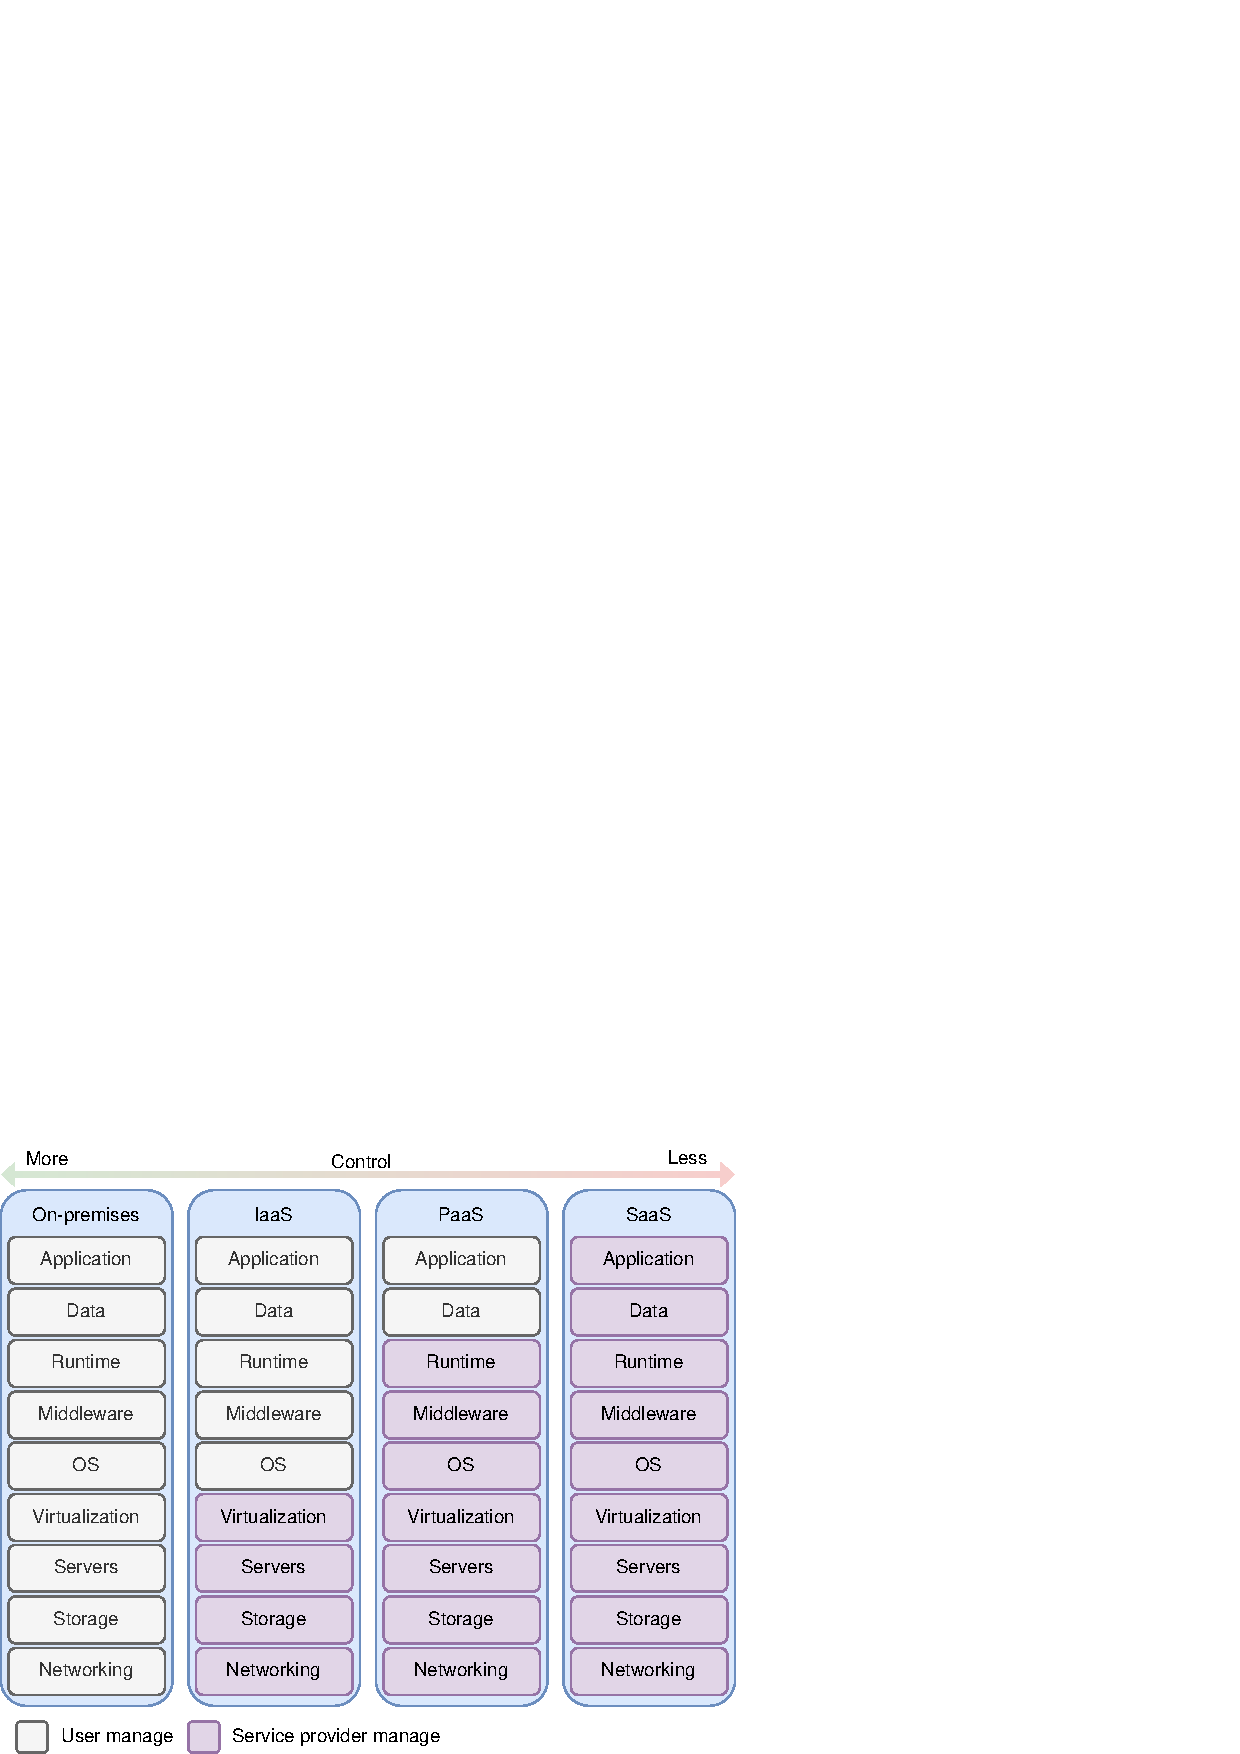
\includegraphics[scale=0.9]{images/Figure1.png}
	\end{center}
	\vspace{-0.6cm}
	\caption{Difference between cloud options and on-premises solution.}
	\label{fig:fig1}
\end{figure}

The user can choose a single solution, or combine more of them if such a thing is required depending on preferences and needs.

By the ownership, CC can be categorized into three categories:

\begin{itemize}
	\item \textbf{Public cloud} is type where CC is delivered over the internet, and shared across many many organizations and users. In this type of the CC, architecture is built and maintained by others. Users and organizations pay for what they use. Examples include: AWS EC2, Google App Engine, Microsoft Azure etc.
	\item \textbf{Private cloud} is type where CC is dedicated only to a single organization. In this type of the CC, architecture is built by organization who may offer their solution or services to the users or other organizations. These services are in domain what the organization does, and that organization is in charge of maintanance. Examples include VMWare, XEN, KVM etc.
	\item \textbf{Hybrid cloud} is such environment that uses both public and private clouds. Examples include: IBM, HP, VMWare vCloud etc.
\end{itemize}

Table~\ref{tab:table4} show comparison of public, private and hybrid cloud capabilities.

\begin{table}[h!]
	\begin{center}
		\begin{tabular}{l|l|l|l}
			\textbf{Capabilities} & \textbf{Public cloud} & \textbf{Private cloud} & \textbf{Hybrid cloud}\\
			\hline
			\textbf{Data control} & IT enterprise & Service Provider & Both \\
			\textbf{Cost} & Low & High & Moderate \\
			\textbf{Data security} & Low & High & Moderate \\
			\textbf{Service levels} & IT specific & Provider specific & Aggregate \\
			\textbf{Scalability} & Very high & Limited & Very high \\	
			\textbf{Reliability} & Moderate & Very high & Medium/High\\	
			\textbf{Performance} & Low/Medium & Good & Good \\
\end{tabular}
	\end{center}
	\vspace{-0.5cm}
	\caption{Comparison of public, private and hybrid cloud capabilities.}
	\label{tab:table4}
\end{table}

In the rest of the thesis, if not stated differently when CC term is used it denotes public cloud.

CC has been the dominating tool in the past decade in various applications~\cite{Satyanarayanan17}. It is changing, evolving, and offering new types of services. Resources such as container as a service (CaaS), database as a service (DBaaS)~\cite{Peter} are newly introduced. The CC model gives us a few benefits. Centralization relies on the economy of scale to lower the cost of administration of big DCs. Organizations using cloud services avoid huge investments. Like creating and maintaining their own DCs. They consume resources usually created by others~\cite{Satyanarayanan17} and pay for usage time -- a pay as you go model. 

But centralization give us few really hard problems to solve. As already stated in section~\ref{sec:problem_area} data is required to be moved to the cloud from data sources, which introduces a high latency in the system~\cite{HossainRH18}. 

There are few notable attempts to help data ingestion into the cloud. Remote Direct Memory Access (RDMA) protocol makes it possible to read data directly from the memory of one computer and write that data directly to the memory of another. This is done by using \textit{specialized hardware} interface cards and switches and software as well, and operations like read, write, send, receive etc. do not go through CPU. With this caracteristivs, RDMA have low latencies and overhead, and as such reach better throughputs~\cite{CohenTKCKRCDG09}. This new hardware may not be cheap, and not evey CC provider use them for every use-case. And this may not be enough, esspecially with ever growing amount of IoT devices and services.

Over the years there are more as a service options avalible, forming \textbf{everything as a service (XaaS)} model~\cite{DuanFZSNH15}. This model propose that any hardware or software resource can be ofered as a service to the users over the internet.

Table~\ref{tab:table2} shows common examples of SaaS, PaaS, and IaaS applications.

\begin{table}[h!]
	\begin{center}
		\begin{tabular}{l|l}
			\textbf{Platform type} & \textbf{Common Examples}\\
			\hline
			\textbf{IaaS} & AWS, Microsoft Azure, Google Compute Engine \\
			\textbf{PaaS} & AWS Elastic Beanstalk, Azure, App Engine \\
			\textbf{SaaS} & Gmail, Dropbox, Salesforce, GoToMeeting \\
		\end{tabular}
	\end{center}
	\vspace{-0.5cm}
	\caption{Common examples of SaaS, PaaS, and IaaS.}
	\label{tab:table2}
\end{table}

CC is giving a user an illusion that he is using single machine, while the backgroud implementaion is fairly complicated and consists of various elements that are composed of countles machines. CC is tipical example of horizontally scalable system presented in~\ref{sec:scalability}
%
%
\subsection{Membership protocol}\label{sec:memership_protocol}
%
A the start of this section we introduced DS, and we present two interesting assumptions by Tanenbaum et al.~\cite{SteenT16, 0019513}. If we take one more look at the~\ref{ds:asumption_2} assumption, we will see that user of the DS whether they are users or applications perceive DS as a single element. Inside this single elements nodes need to colaborate, so that they are albe to do various kinds of tasks.

Most basic of all these tasks, is that nodes needs to know which group they belog to, and who are their peers in the group they will colaborate with. This might sound as a trivial idea, but when we include 8 fallacies of the DS~\ref{ds:8_fallacies} into the equation, things start to be not so trivial, after all. In the setup where nodes are connected over the local network or internet, and they need to communicate things will go wrong for various reasons.

To resolve the problem that nodes need to know who are their group peers, a membership protocols come to help. These protocols needs to ensures that each process of one group updates his local list of \textbf{non-faulty} members of the group, and when a new process joins or leaves the group, local list for every process needs to be updated. This is the most basic idea behind membership protocols.

Processes in the group, or nodes in a group will ping each other in different ways, and using different strategies to figure out which nodes are dead and which are alive. There are few existing algorithms that does this job, and they are (usually) based on the way epidemics spread or how gossip is spreaded in population. Because of this feature these algorithms are usually called \textit{Gossip} style protocols.

Every membership protocol have some properties that will ensure efficiency and scalability:

\begin{enumerate}[start=1,label={(\bfseries \arabic*)}] \label{ds:features}
	\item \textbf{Completeness}, this property must ensure that every failure in the system is detected.
	\item \textbf{Accuracy}, in ideal world, there should be no mistakes when detecting failures. But In real life scenario, we need to reduce false positives as much as we can.
	\item \textbf{Failure detection speed}, all failures needs to be tected as fast as possible, in order to remove the node from the group and reschedule the tasks from dead node to alive ones.
	\item \textbf{Scale}, with this property we must ensure that the network load that is generated should be distributed equally between all processes in the group.
\end{enumerate}

Easiest idea to implement this protocol would be \textbf{heartbeating} technique where process $P_i$ will send heartbeat message to all his peers in the group or \textbf{multicast}. After some time if process $P_j$ did not receive heartbeat message from $P_i$, it will mark him as faild. This idea is easy to understand, and implement but downsides are that his process is not really \textbf{scalable}, esspecially for large groups, and this will introduce huge network traffic.

To resolve this problem, Das et al.~\cite{DasGM02} introduced \textbf{S}calable \textbf{W}eakly-consistent \textbf{I}nfection-style Process Group \textbf{M}embership protocol, or \textbf{SWIM} for short. This protocol divides the membership problem into two parts:

\begin{enumerate}[start=1,label={(\bfseries \arabic*)}]
	\item \textbf{Failure detection}, this component works so that one node will select random node in the group, and it will send him $ping$ message, expecting $ack$ message in return --- \textbf{direct ping}. If such message is not received, he will pick $n$ nodes to probe through a $ping-req$ message --- \textbf{indirect ping}. If this fail, node will be marked as $suspected$, and it will be marked as $dead$ after some timeout. If node get alive, he will ping some other node and he will get back into the group. Figure~\ref{fig:fig15} show message passing in \textbf{direct} $(left)$, and \textbf{indirect} $(right)$ ping in SWIM protocol.
	\item \textbf{Information dissemination}, with previous strategy, we can disseminate information by piggybacking the data on multiple messages ($ping$, $ping-req$ and $ack$), and avoid using the multicast solution.
\end{enumerate}

\begin{figure}[H]
	\begin{center}
		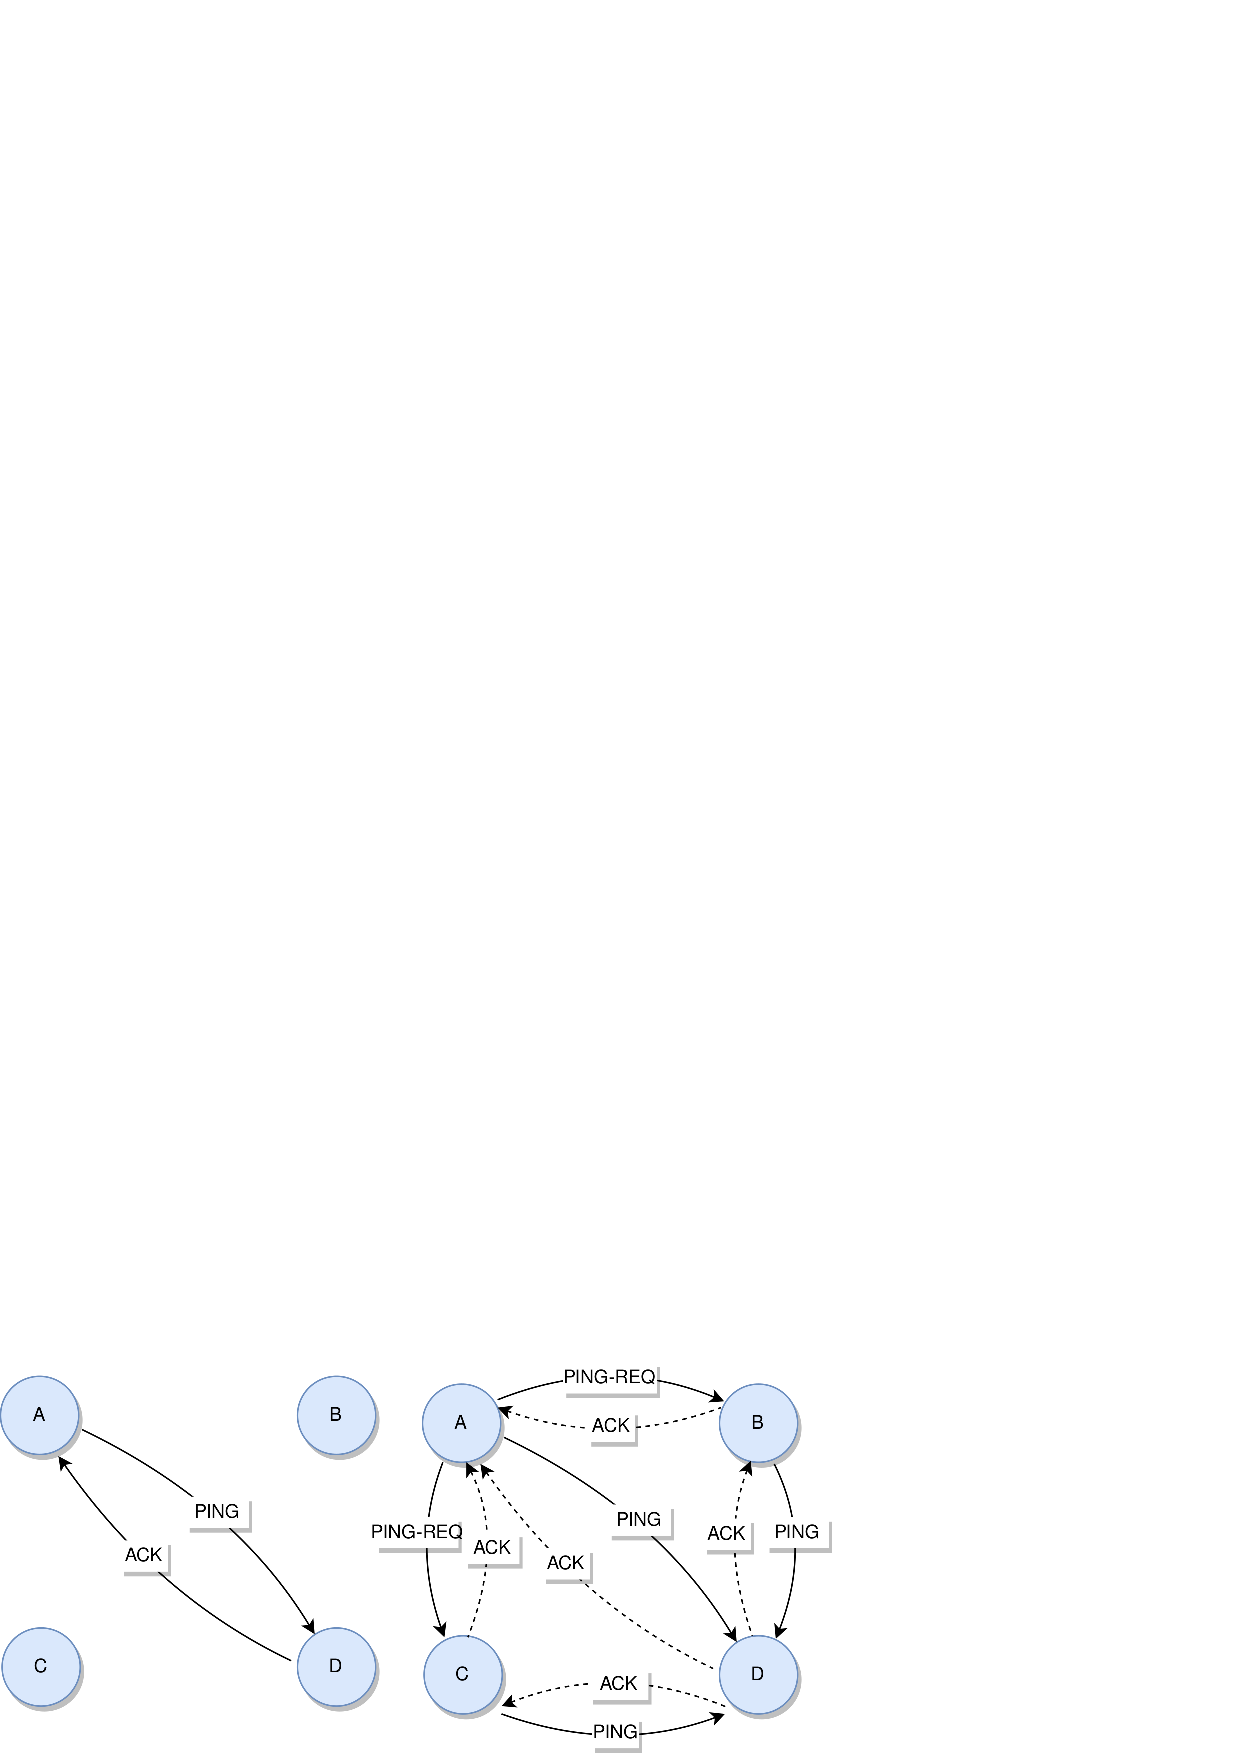
\includegraphics[scale=0.7]{images/Figure15.png}
	\end{center}
	\vspace{-0.6cm}
	\caption{Direct and indirect ping in SWIM protocol.}
	\label{fig:fig15}
\end{figure}

Over the years, reserchers foud ways to improve the protocol for example Dadgar et al. present Lifeguard protocol~\cite{DadgarPC18} for more
acccurate failure detection, and there are other implementations to fine tune the SWIM, but base idea is still there. Today SWIM or SWIM-like protocols are standard membership procol whenever we are doing some node clustering.
%
%
\subsection{Mobile computing}\label{sec:mobile_computing}
%
Mobile cloud computing (MCC), was the first idea that introduced task offloading~\cite{FernandoLR13, LinLJL19}. Heavy computation remains in the cloud. Mobile devices run small client software and interact with the cloud, over the internet using his resources. 

The main problem with MCC is that the cloud is usually far away from end devices. That leads to high latency and bad quality of experience (QoE)~\cite{LinLJL19}. Especially for latency-sensitive applications. Even though MCC is not that much different from the standard cloud model. We had moved a small number of tasks from the cloud. Thus opening the door for future models.

To overcome cloud latency and MCC problems, research led to new computing areas like edge computing (EC). EC is a model in which computing and storage utilities are in proximity to data sources~\cite{Satyanarayanan17}. The cloud is enhanced with new ideas for future generation applications~\cite{NingLSY20}. 

Over the years, designs like fog~\cite{BonomiMNZ14}, cloudlets~\cite{MonsalveCC18}, and mobile edge computing (MEC)~\cite{WangZZWYW17} emerged. In this thesis, we refer to all these models as edge nodes. They all use the concept of data and computation offloading from the cloud closer to the ground~\cite{KhuneP19}, while heavy computation remains in the cloud because of resource availability~\cite{NingLSY20}. 

EC models introduce small-scale servers that operate between data sources and the cloud. Typically, they have much less capabilities compared to the cloud counterparts~\cite{ChenHLLW15}. These servers can be spread in base stations~\cite{WangZZWYW17}, coffee shops, or over geographic regions to avoid latency as well as huge bandwidth~\cite{MonsalveCC18}. They can serve as firewalls~\cite{SatyanarayananK19} and pre-processing tier, while users get a unique ability to dynamically and selectively control the information sent to the cloud.
%
%
\section{Distributed computing}\label{sec:distributed_computing}
%
DC can be defined as the use of a DS to solve one large problem by breaking it down into several smaller parts, where each part is computed in the individual node of the DS and coordinatio is done by passing messages to one another~\cite{0019513}. Computer programs that use this strategy and runs on DS are called \textbf{distributed programs} \cite{Vera16, andrews2000foundations}. 

Similar to CC in Section~\ref{sec:cloud_computing}, to a normal user, DC systems appear as a single system similar to one he use every day on his personal computer. DC share same fallacies to DS presented in~\ref{sec:distributed_systems}.
%
%
\subsection{Big Data}\label{sec:big_data}
%
Tearm big data means that the data is unable to be handled, processed or loaded into a single machine~\cite{FisherDCD12}. That menas that traditional data mining methods or data analytics tools developed for a centralized processing  may not be able to be applied directly to big data~\cite{Tsai2015}. 

New tools and methos that are developed are relying on DS and one specific feature \textbf{data locality}. Data locality can be described as a process of moving the computation closer to the data, instead of moving large data to computation~\cite{GuoFZ12}. This simple idea, minimizes network congestion and increases the overall throughput of the system.

In~\ref{sec:problem_area} we already give two examples how huge generated data could be, and when we incude other IoT sensors and devices these numbers will just keep getting bigger~\cite{SarigiannidisLR20}.

On contrary to relational databases that mostly deal with structured data, big data is dealing with various kinds of data~\cite{FisherDCD12, Tsai2015, GuoFZ12}:

\begin{itemize}
	\item \textbf{Structured} data is kind of data that have some fixed structure and format. Tipical example of this is data stored inside table of some database. organizations susully have no huge problem extracting some kind of value out of the data.
	\item \textbf{Unstructured} data is kind of data where wo do not have any kind of structure at all. These data sources are heterogeneous and may containing a combination of simple text files, images, videos etc. This type of data is usully in raw format, and organizations have hard time to derive value out.
	\item \textbf{Semi-structured} data is kind of data that can contain both previously mentioned types of data. Example of this type of data is XML files.
\end{itemize}

Along it's share size, big data have other instantly recognizable features called \textbf{V's} of big data~\cite{PatgiriA16}. Name is derived from starting letters from the other features that are describing big data. Image~\ref{fig:fig3} show 6 V's comonly used to represent the big data.

\begin{figure}[H]
	\begin{center}
		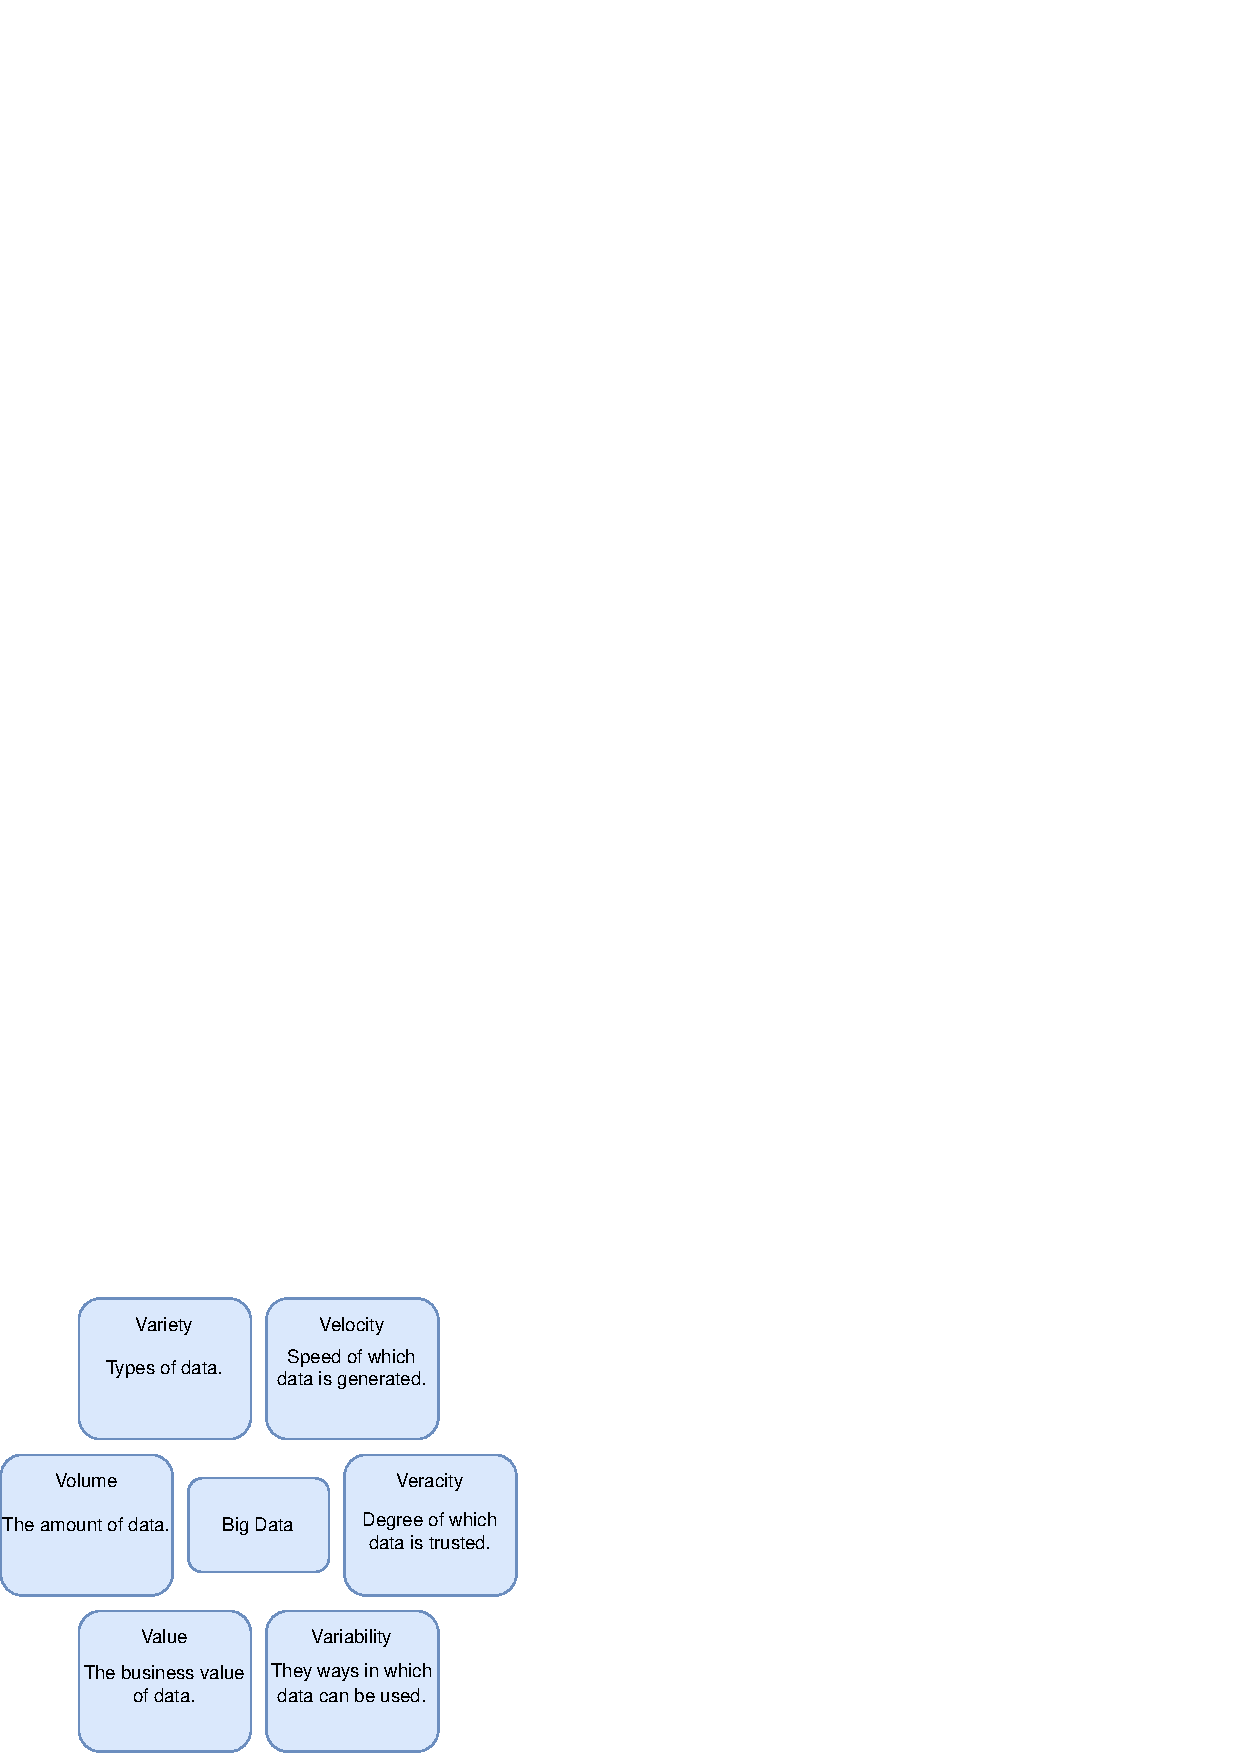
\includegraphics[scale=0.7]{images/Figure3.png}
	\end{center}
	\vspace{-0.6cm}
	\caption{V's of Big Data.}
	\label{fig:fig3}
\end{figure}

Processing in big data systems can be represented as~\cite{phdthesis, KiranMMDB15}:

\begin{itemize}
	\item \textbf{Batch processing} represents data prcessing technique that is done on huge quantity of the stored data. This type of prcessing is usually slow and requure time.
	\item \textbf{Stream processing} represents data processing technique that is done as data get into the system. This type of processing is usually done on smaller quantity of the data \textbf{at the time}, and it is faster.
	\item \textbf{Lambda architectures} represents processing technique where stream processing and handling of massive data volumes in batch are combined in a uniform manner, reducing costs in the process~\cite{KiranMMDB15}.
\end{itemize}

Big data systems, are not processing and value extracting systems. Big data systems can be separated in few categories: $(1)$ data storage, $(2)$, data ingestion $(3)$, data processing and analytics. All these system aids to properly analyze ever growing requirements~\cite{RaoMBG19},

Dispite promise that big data offers to derive value out of the collected data, this task is not easy to do and requre properly set up system filtering and removeing data that contains no value. To aid this idea, data could be filtered and little bit preprocessed on close to the source~\cite{inproceedingsSimic1}, and as such sent to data lakses~\cite{MarynowskiSP15}.
%
%
\subsection{Microservices}\label{sec:microservices}
%
There is no single comperhensive deffinition of what a microservice is. Differnet people and organizations use different definition do describe them. A working definition is offered in~\cite{DragoniGLMMMS16} as~\say{s microservice is a cohesive, independent process interacting via messages}. Despite lack of comperhensive definition all agree on few features that come with microservices: 

\begin{enumerate}[start=1,label={(\bfseries \arabic*)}]
	\item they are small computer programs that are independently deployable and developed.
	\item they coud be developed using different languages, principles and using differend databses.
	\item they communicate over the network to achieve some goal.
	\item they are organized around business capabilities~\cite{PautassoZALJ17}.
	\item they are implemented and mainteined by a small team.
\end{enumerate}

Industry is migrating much of their applications to the cloud, because CC offers to scale their computing resources as per their usage~\cite{LiZJLZLGGS19}. Microservices are small loosely coupled services that follos UNIX philosophy~\say{do one thing, and do it well}~\cite{krause2015microservices}, and they communicate over well defined API~\cite{DragoniGLMMMS16}.

This architecure patter is well aligned to the CC paradigm~\cite{LiZJLZLGGS19}, contrary to previous models like monolith whose modules cannot be executed independently~\cite{DragoniGLMMMS16, abs-1905-07997}, and are not well aligned with the CC paradigm~\cite{abs-1905-07997}. Table~\ref{tab:table3} summrize differences between monolith and microservie architecture.

\begin{table}[h!]
	\begin{center}
		\begin{tabular}{l|l|l}
			\textbf{Feature} & \textbf{Monolith} & \textbf{Microservices}\\
			\hline
			\textbf{Structure} & Single unit & Independent services \\
			\textbf{Management} & Usually easier & Add DS complexity\\
			\textbf{Scale/Update} & Entire app & Per service \\
			\textbf{Error} & Usually crush entire app & App continue to work \\
		\end{tabular}
	\end{center}
	\vspace{-0.5cm}
	\caption{Differences between horizontall and verticall scaling.}
	\label{tab:table3}
\end{table}

Since their inception, microservices architecture is gone through some adaptations. And modern day microservices are extended with two new models each with it's unique abilities and problems:

\begin{itemize}
	\item \textbf{Cloud-native applications}, are specially designed applications for CC. They are distributed, elastic and horizontal scalable system by their nature, and composed of (micro)services which isolates state in a minimum of stateful components~\cite{KratzkeQ17}. These type of applications are self-contained, could be deployed independently, and they are composed of loosely coupled microservices that are packaged in lightweight containers. They have Improved resource utilization, and they are centered around APIs.
	\item \textbf{Serversles applications} is computing model, where the developers need to worry only about the logic for processing client requests~\cite{AdzicC17}. Logic is represented as event handler that only runs when client request is received, and billing is done only when these functions are executing~\cite{AdzicC17}. \textbf{Cold start} is one of features of the severless computing, and we can define it as user requests need to wait, until new container instance is up and running before can do any processing at all. Most providers have 1–3 second cold starts, and this is important for certain types of applications where latency is concern. Cold start is only happening when there are no \textit{warm} containers available for the request, meaning there is no single instance to server request. Other features include: $(1)$ simplified services development, $(2)$ faster time to market, $(3)$ and lower costs.
	\item \textbf{Service Mesh} is designed to standardize the runtime operations of applications~\cite{LiLGZH19}. As part of the microservices ecosystem,
	this dedicated communication layer can provide a number of benefits, such as: $(1)$ observability, $(2)$ providing secure connections, or $(3)$ automating retries and backoff for failed requests. With these features, developers only focus on implementation of buisniss logic, while operators gain out-of-the-box traffic policies, observability, and insights from the services. Advocates of microservice movemant, nowdays recommend using service mesh architecture when running microservices in production environments.
\end{itemize}

Microservices communicate over a network to fulfil some goal using message passing technique and technology-agnostic protocols such as HTTP. They can be implemented as:

\begin{itemize}
	\item Representational state transfer (REST) services~\cite{AdamczykSJH11}, is an architectural style with set of constraints that users can create web srevices and interoperability between computer systems on the internet. It is based on HTTP routs to define resources, and used HTTP verbs to represent operations over these resources. It relys on textual based communications, and payload could be represented using $JSON$, $XML$, $HTML$ etc.
	\item Remote procedure calls (RPC) represent architectural way to design services that are able to call subroutines that are located in different places, usually on other machine. Client is calling these operations like they are located localy in his address space.
	\item Event-driven services, are services where communicatoin between services is done using events. Events are sent on some channel and other read messages that are received on other channel. These channels could be implemented either like message queues or message topics. Services connect to message queu or subscribe to the specific topic, and when messige arive, they can act acording to message type.
\end{itemize}
 
 They are well aligned with text based protocols like HTTP/1 using $JSON$ for example, or binary protocols such as HTTP/2 using $protobuf$ and $gRPC$ for example, and even new faster version like HTTP/3 over new $QUIC$ protocol, designed by Google. HTTP 3 is the latest version of the conventional and trusted HTTP protocol. It is very similar to HTTP 2, but it also offers a few important new features. Table~\ref{tab:table9} show important difference between versions of HTTP protocol.
 
 \begin{table}[h!]
 	\begin{center}
 		\begin{tabular}{l|l|l|l}
 			\textbf{Feature} & \textbf{HTTP1} & \textbf{HTTP2} & \textbf{HTTP3}\\
 			\hline
 			\textbf{Transport} & text & binary & binary\\
 			\textbf{Parallelism} & No & Yes & Yes\\
 			\textbf{Protocol} & TCP & TCP & QUIC \\
 			\textbf{Space} & OS level & OS level & User level\\
 			\textbf{Server push} & No & Yes & Yes\\
 			\textbf{Compression} & Data & Data/Headers & Data/Headers\\
 		\end{tabular}
 	\end{center}
 	\vspace{-0.5cm}
 	\caption{Idempotent and non-idempotent operations.}
 	\label{tab:table9}
 \end{table}
 
 To enshure vider range of devices that are able to comunicate with the rest of the systems, developrs usually have a gateway into the system that is REST service, and other services could be implemented in different way.

It is important to point out, that all flavors of microservices applications rely on continuous delivery and deployment~\cite{7436659}. This is enabled by lightweight containers, instead of virtual machines~\cite{FelterFRR15}, and orchestration tools such Kubernetes~\cite{BurnsGOBW16}. These concepts wll be described in more detail in Section~\ref{sec:virtualization_techniques}.

Microservices architecture are good starting point especially for build as a service applications, and applications that should serve huge amount of requests and users. Esspecially with benefits of CC to pay for usage, and ability to scale parts of the system independently.  Although they are not necessarily easy to implement properly. There are more and more critique to the architecture model~\cite{SoldaniTH18}. Microservices are relying and use parts of the DS, and as such they inherit almost all problems DS has. 

One particilar thing that users need to be aware of is \textbf{idempotency}. In microservices applications, developers are dealing with inconsistencies in distributed state, and their operations should be implemented as idempotent. An operation is idempotent if it will produce the same results when executed over and over again. It is a strategy that means that operations with sade effects like creation or deletion can be called any number of times, while guaranteeing that side effects only occur once. Idempotency is term that come from mathematics, and can be represented by simple idempotency law for operation $*$ like~\cite{gratzer2002general}:

\begin{equation}\label{form:idempotency_law}
	\forall x, x * x = x
\end{equation}
\myequations{Idempotency law formula}

Not all Create, Read, Update, Delete (CRUD) operations are idempotent by default. But developers need to make effort to make all of them idempotent, to prevent bad outcomes and incosistant state. 

Table~\ref{tab:table8} show list of idempotent and non-idepotent for standard CRUD operations:

\begin{table}[h!]
	\begin{center}
		\begin{tabular}{l|c|c}
			\textbf{Operation} & \textbf{Idempotent} & \textbf{Non-idempotent}\\
			\hline
			\textbf{Create} &  & x \\
			\textbf{Read} & x & \\
			\textbf{Update} & x & \\
			\textbf{Delete} & x & \\
		\end{tabular}
	\end{center}
	\vspace{-0.5cm}
	\caption{Idempotent and non-idempotent operations.}
	\label{tab:table8}
\end{table}

Crate operation is not idempotent by default, but to make it idempotent there are multiple strategies how to do so. Most comon way is to create \textbf{idempotency key} that will be sent in the request, and based on that request server can decide is this operations already invoked or not. If server is already \say{seen} specified idempotency key, than operation is already done and we can return just responce that operation is done but no operation will be done over the state of the service or application. If server see idempotency key for the first time, that is the signal that this request is new one, and it should be done.

Idempotency key could be stored in any kind of the storage, it is not uncommon that these keys are stored in cache storage with some time to live (TTL) policy that will automatically remove the key after specified time.

Other option that is comonly used is hasing user specified actions. This is usefull to know what part of action set is already done and what is not. This strategy is used in scenarios where we must preserve order of actions.

Best chance to success when implementing microservices architecture, is to simply follow existing patters and use existing solutions with proven quality.
%
%
\section{Distribution Models}\label{sec:distribution_models}
%
The role of distribution models is to determine the responsibility for the request, or to answer the fundamental question \say{who is in charge} for specific request. There are two ways to answer this question: $(1)$ all nodes in the system, or $(1)$ single node in the system.
%
%
\subsection{Peer-to-peer}\label{sec:p2p_networks}
%
Peer-to-peer (P2P) communication is a networking architecture model that partitions tasks or workloads between peers~\cite{Schollmeier01}. All peers are created equally in the system, and there is no such thing as a node that is more important then others. Every Peer have a portion system resources, such as processing power, disk storage or network bandwidth, directly available to other network participants, without the need for central coordination by servers or stable hosts~\cite{Schollmeier01}. P2P nodes are connected and share resources without going through a separate server computer that is responsabile for routing. Figure~\ref{fig:fig2} show difference in network topology between P2P networks $(left)$ and client-server architecture $(right)$.

\begin{figure}[H]
	\begin{center}
		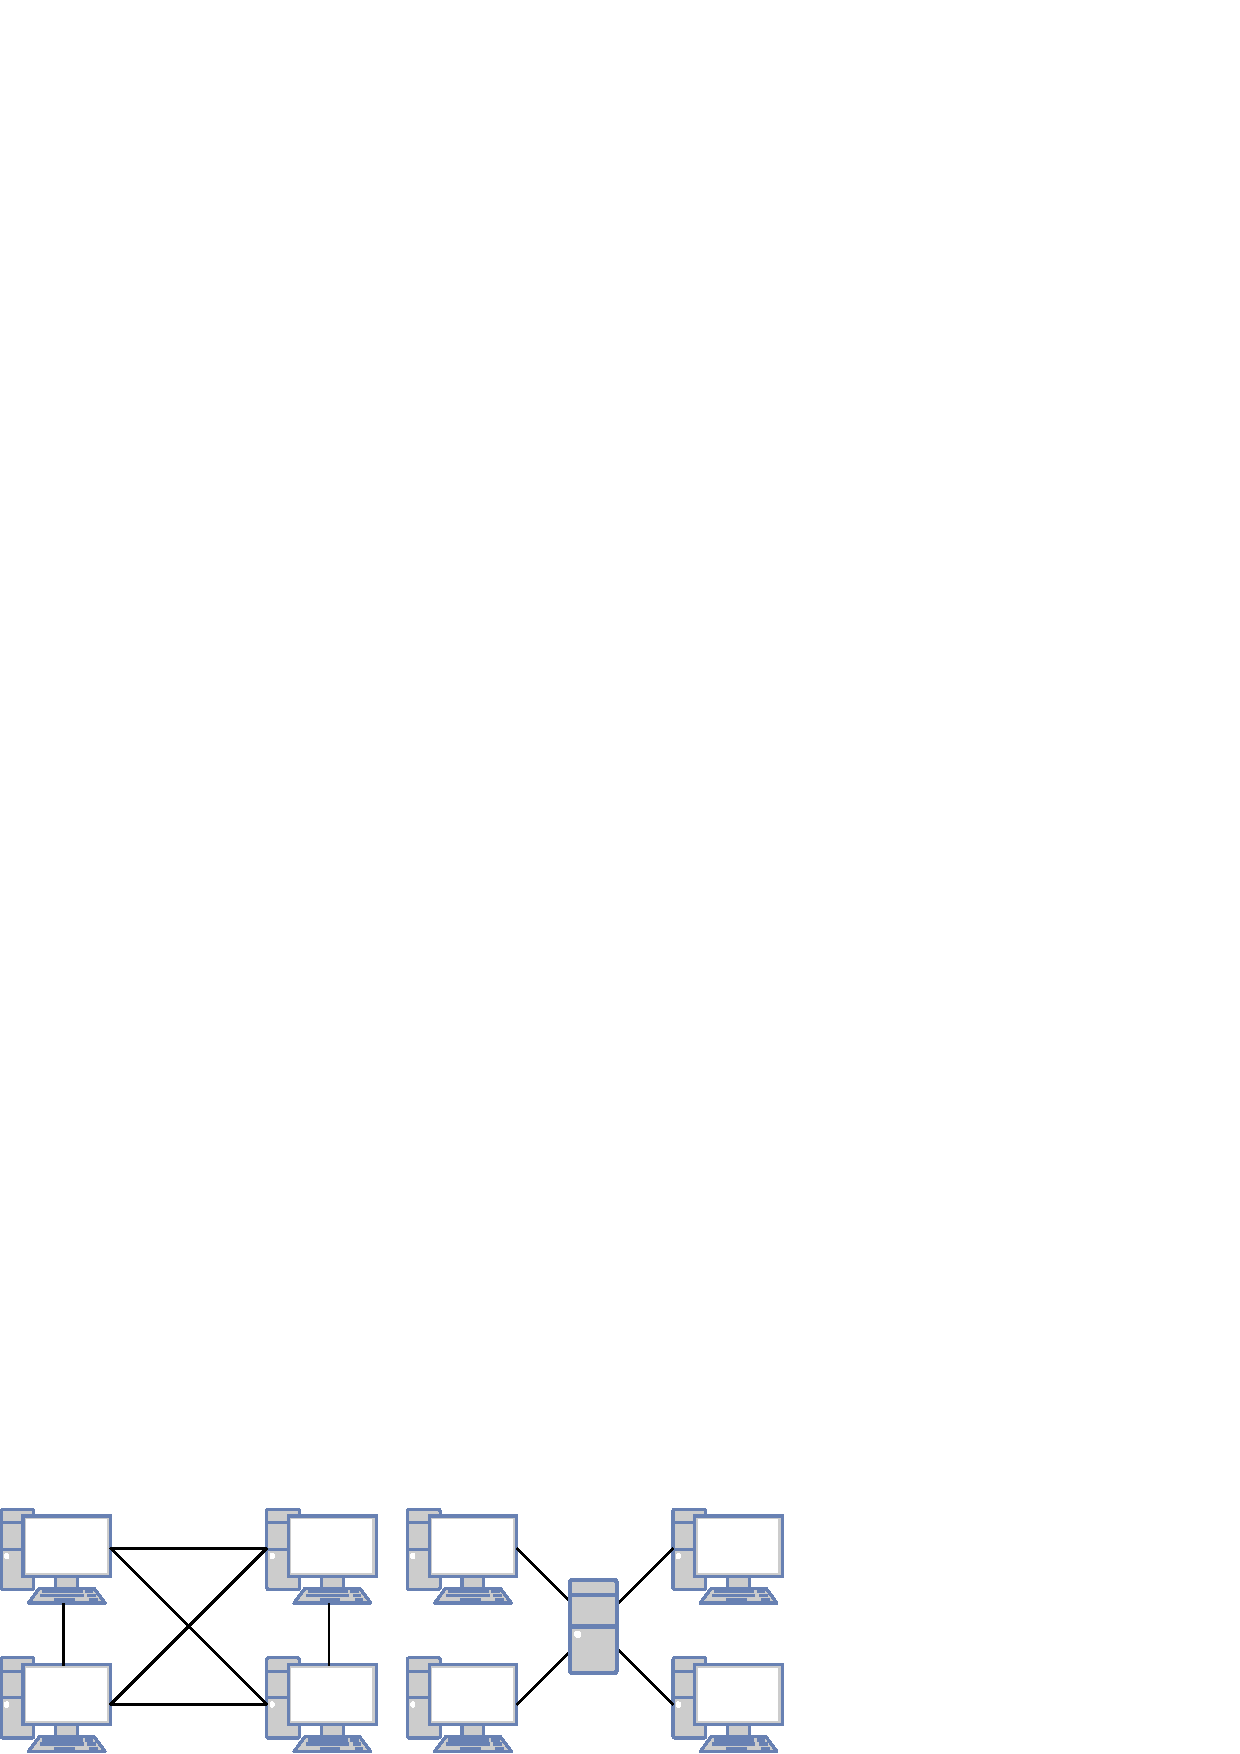
\includegraphics[scale=0.7]{images/Figure2.png}
	\end{center}
	\vspace{-0.6cm}
	\caption{P2P network and client-server network.}
	\label{fig:fig2}
\end{figure}

Peers are creating a sense of virtual community. This community of peers can resolve a greater tasks, beyond those that individual peers can do. Yet, these tasks are beneficial to all the peers in the system~\cite{BandaraJ13}. When request come to such network, node that accepted request is usually called \textbf{coordinator}, because he then is trying to found the right peer to send request to.

Based on how the nodes are linked to each other within the overlay network, and how resources are indexed and located, we can classify networks as~\cite{KamelSE07}:

\begin{itemize}
	\item \textbf{Unstructured} do not have a particular structure by design, but they are formed by nodes that randomly form connections~\cite{FilaliBHB11}. Their strenght and weaknes at the same time is ther lack of structure. These networks and robust when peers join and leave network. But when doing query, they must found more possible peers that have same peace of data. Tipical example of this group is a Gossip-based protocols like~\cite{DasGM02}.
	\item \textbf{Structured} peers are organized into a specific topology, and the protocol ensures that any node can efficiently search the network for a resource. The famos type of structured P2P network is a Distributed Hash Table (DHT). These networks maintain lists of neighbors to do more efficent lookup, and as such they are not so robust when nodes join or leave the network. DHT commonly used in resource loopkup systems~\cite{StoicaMKKB01}, and as efficent resource lookip management and scheduling of applications, or as an integral part of distributed storage systems and NoSQL\cite{Leavitt10} databases.
	\item \textbf{Hybrid} combine previous two models in various ways.
\end{itemize}

P2P networks are great tool in many arsenals, but because their unique ability to act as a server and as a client at the same time we must be aware and pay more attention to security because they are more vulnerable to exploits~\cite{0024003}.
%
%
\subsection{Master-slave}\label{sec:master_slave}
%
In the master-slave architecture, there is one node that is in charge -- \textbf{master}. This node accespt requests, and we usually do not communicate to rest of nodes or \textbf{slaves}. Master node is usually better and more expensive or even specialized hardware such as RAID drives to lower the crush probability. The cluster can also be configured with a \textbf{standby} master, and this node is continually updated from the master node.

But no metter how specialized hardware master runs on, it is prone to fail for varios reasons, so he is a \textbf{single point of failure}. If crush happend, than standby master could continue to server as a master, or new \textbf{leader election} protocol~\cite{KorachKM90} is initiated to pick new master node. 

Master node is responsible for processing any updates to that data. If the master fails, than  the slaves can still handle read requests. Failure of the standby master node, to take over from the master node is a real problem if we want to achieve high-availability system.

Figure~\ref{fig:fig16} show difference between mater-slave $(left)$ and peer-to-peer $(right)$ request handling.

\begin{figure}[H]
	\begin{center}
		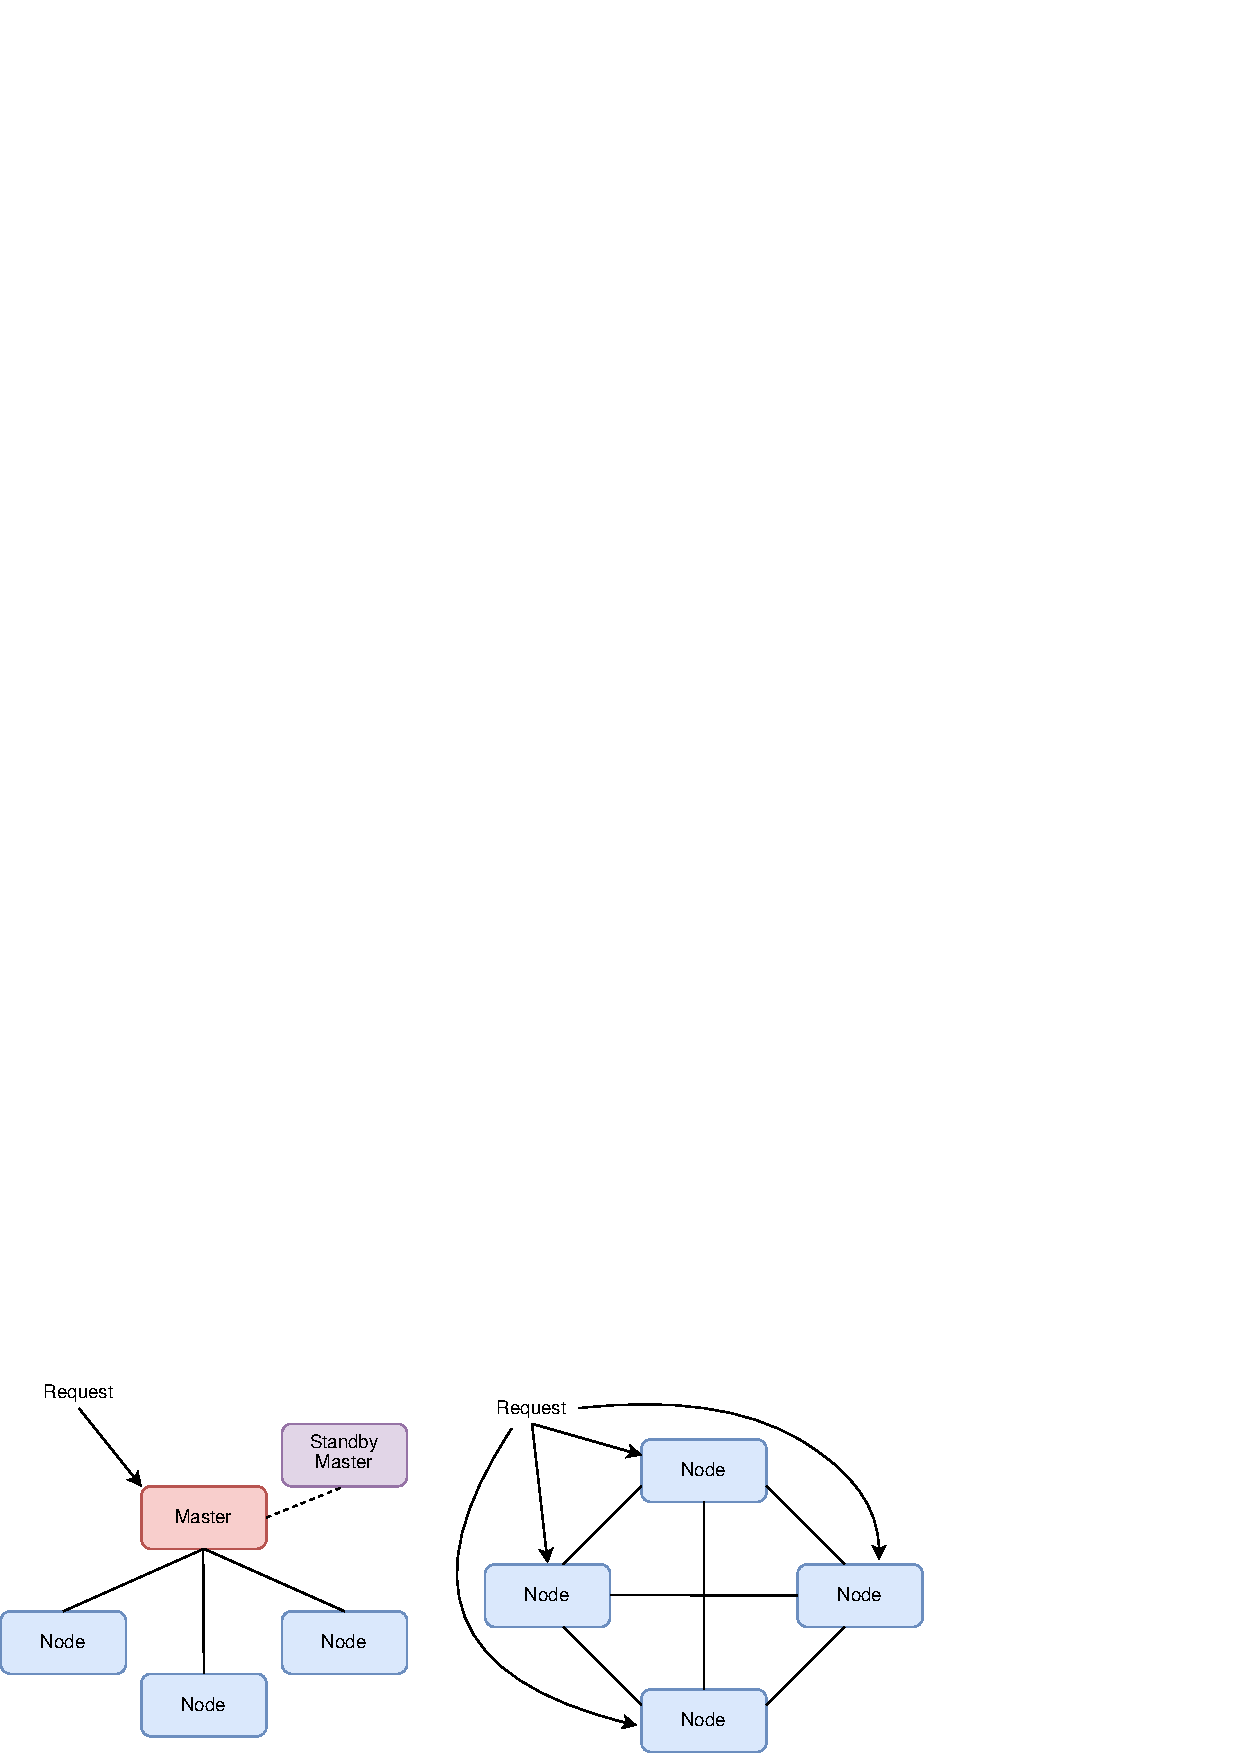
\includegraphics[scale=0.7]{images/Figure16.png}
	\end{center}
	\vspace{-0.6cm}
	\caption{Handling requests master-slave and peer-to-peer}
	\label{fig:fig16}
\end{figure}

Using the right distribution model usually depends on the business requirements. High availability requires a P2P network because no single point of failure. If we could manage data using batch jobs that run in off hours, then the simpler master-slave model might be the solution.
%
%
\section{Similar computing models}\label{sec:similar_models}
%
In this section we are going to shortly describe models that are similar to the DS, and as such they may be the source of confusion.
%
%
\subsection{Parallel computing}\label{sec:parallel_computing}
%
DC and parallel computing seems like models that are the same, and that may share some features like simultaneously executing a set of computations in parallel. Broadly speaking, this is not far from the truth~\cite{Vera16}. 

Distinguished between the two can be presented as follows: in parallel computing all processor units have acces to the shared memory and have some way of the faster inter-process communication, while in DS and DC all processors have their own memory on their own machine and communicate over network to other nodes which is significantly slower. 

These models are similar, but they are not indentical, and the kind of problems they are designed to work on are different. Figure~\ref{fig:fig4} visually summarize the architectural  differences between DC $(up)$ and parallel computing $(down)$.

\begin{figure}[H]
	\begin{center}
		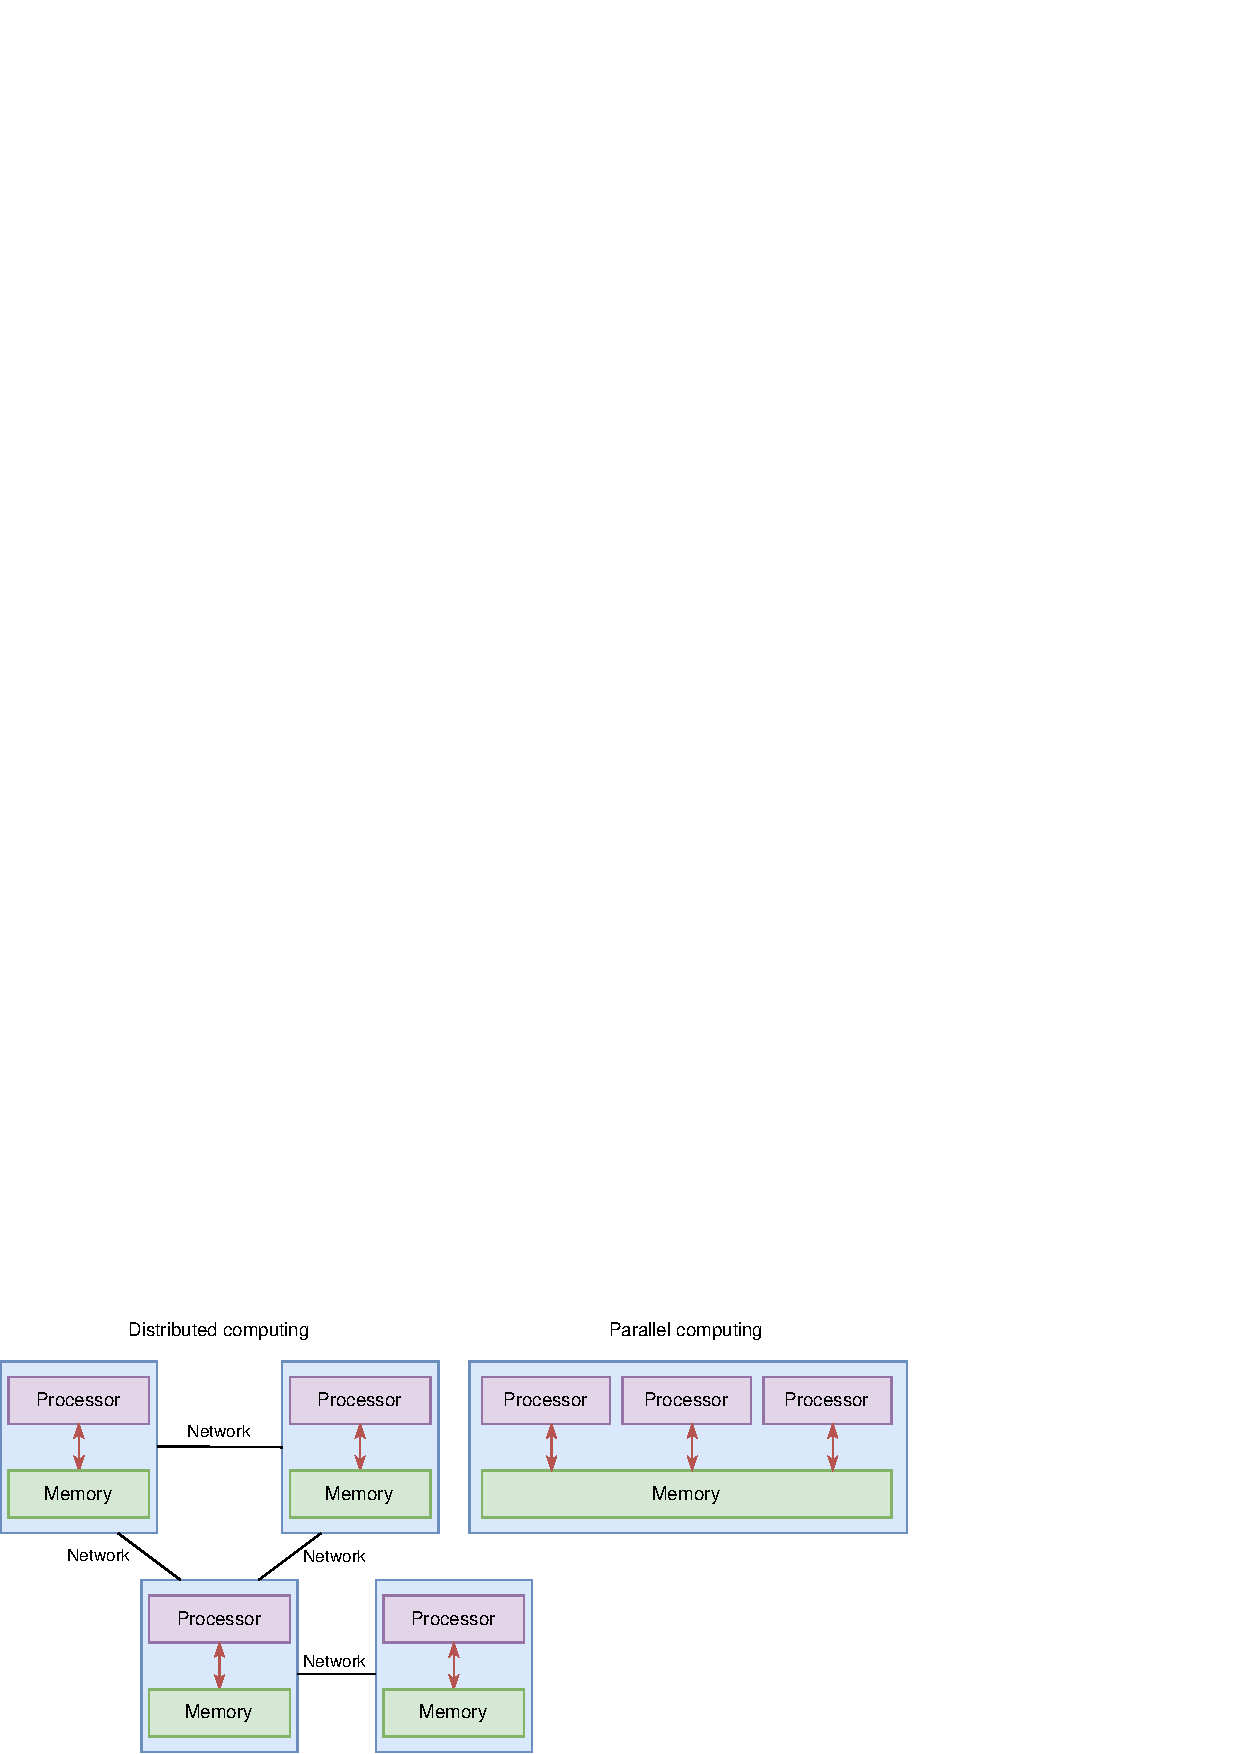
\includegraphics[scale=0.8]{images/Figure4.png}
	\end{center}
	\vspace{-0.6cm}
	\caption{Architectural difference between DC and parallel computing.}
	\label{fig:fig4}
\end{figure}

Parallel computing is often used strategy with problems, that due to their nature or constraints must be done on multi-core machines simultaneously~\cite{0072397}. It is ofthen, that huge problems are divided into smaller ones, which can then be solved at the same time. 

There are number of tasks that requre parallel computing like simulations, computer graphics rendering or different scenarios in scientific computing.
%
%
\subsection{Decentralized systems}\label{sec:decentralized_systems}
%
Decentralized systems are similar to DS, in technical sense they are still DS. But if we take closer look, these systems \textbf{should not} be owned by the single entity. CC for example is perfect example of DS, but it is not decentralized by it's nature. It is centralized systems by the owner like AWS, Google, Microsoft or some other private compay because all computation needs to be moved to big DCs~\cite{HossainRH18}.

By today standards, when we are talking about decentralyzed systems, we usually think of blockchain or blockchain-like technology~\cite{LeibleSSG19}. Since here we have distributed nodes, that are scattered and there is no single entity that own all these nodes. But even if this technology is run in the cloud, it is loosing the decentralized feature. This is the caveat we needs to be aware of. These systems are facing different issues, because any participent in the system might be malicious and they need to handle this case. 

Nontheless, CC can and should be decentralized in a sense that some computation can happend outside of cloud big DCs, closer to the sources of data. These computation could be owned by someone else, and big cloud companies could give their own solution to this as well to relax centralization and problems that CC will have esspecially with ever growing IoT and mobile devices.
%
%
\section{Virtualization techniques}\label{sec:virtualization_techniques}
%
Virtualization as a technique started long ago in time-sharing systems, to provide isolation between multiple users shareing a single system liek a mainframe computer~\cite{CrosbyB06}. 

In~\cite{Sharma} Sharma et al. describe virtualization as technologies which provide a layer of abstraction of the physical computing resources between computer hardware systems and the software systems running on them.

Modeern virtualization diferentiate few different tools. Some of them are used as an integral part of the infrastructure for some flavors like IaaS, while others are used in different CC flavors as well as microservices packageing and distribution format, or are new and still are looking for their place. These options are:

\begin{itemize}
	\item \textbf{Virtual machines (VM)} are the oldest tehnology of the three. In~\cite{Sharma} Sharma et al. describe them as a self-contained operating environment consisting of guest operating system and associated applications, but independent of host operating system. VMs enable us to pack isolation and better utilization of hardware in big DCs. They are vidly used in IaaS environment~\cite{AbsalomBJ13, YangHCLW13} as a base where users can install theirown operating system (OS) and required software tools and applications.
	\item \textbf{Containers} provide almost same functionality to VMs, but there are several subtle differences that make them a goto tool in modern develpment. Instead of the guest OS running on top of host OS, containers use tools that are in Linux kernles like \textit{cgroups} that limits process resource usage so that single process can not starve other processes and use all the resources for himself, and \textit{namespaces} to provide isolation and partitions kernel resources so that single process see node resources like he only exists there. Containers reduce time and footprint from development to testing to production, and they utilize even more hardware resources compared to VMs and show better performance compared to the VMs~\cite{Seo2014PerformanceCA, FelterFRR15}. Containers provide easier way to pack servies and deploy and they are esspecially used in microservices architecture and service orchestration tools like Kubernetes~\cite{BurnsGOBW16}. Google stated few times in their on-line talks that hey have used container technology for all their services, even they run VMs inside containers for their cloud platform. Even though they exist for a while, containers get popularized when companies like Docker and CoreOS developed user-friendly APIs.
	\item \textbf{Unikernels} are the newest addition to the virtualization space. In~\cite{pavlicek2016unikernels} Pavlicek define unikernels as small, fast, secure virtual machines that lack operating systems. Unikernels are comprised of source code, along with only the required system calls and drivers. Because of their specific design, they have single process and they contains and executes what it absolutely needs to nothing more and nothing less~\cite{GoethalsSAVT18}. They are advertised that new technology that will safe resources and that they are \textit{green}~\cite{208735} meaning they save both power and money. When put to the test and compared to containers they give interesting results~\cite{GoethalsSAVT18, PlauthFP17}. Unikernels are still new technology and they are not widly adopted yet. But they give promessing features for the future, esspecially \textbf{if} properly ported to ARM architectures, and various development languages. Unikernes will probably be used as a user applications and functions virtualization tool, because their specific architecture, esspecailly for serverless applications presened in~\ref{sec:microservices}.
\end{itemize}

Figure~\ref{fig:fig5} represent architectural differences between VMs, containers and unikernels.

With every virtualization technique, ultimate goal is to pack as much applications on existing hardware as possible, so that there is no resources that are left not used --- we are trying to achieve high resource utilization.

\begin{figure}[H]
	\begin{center}
		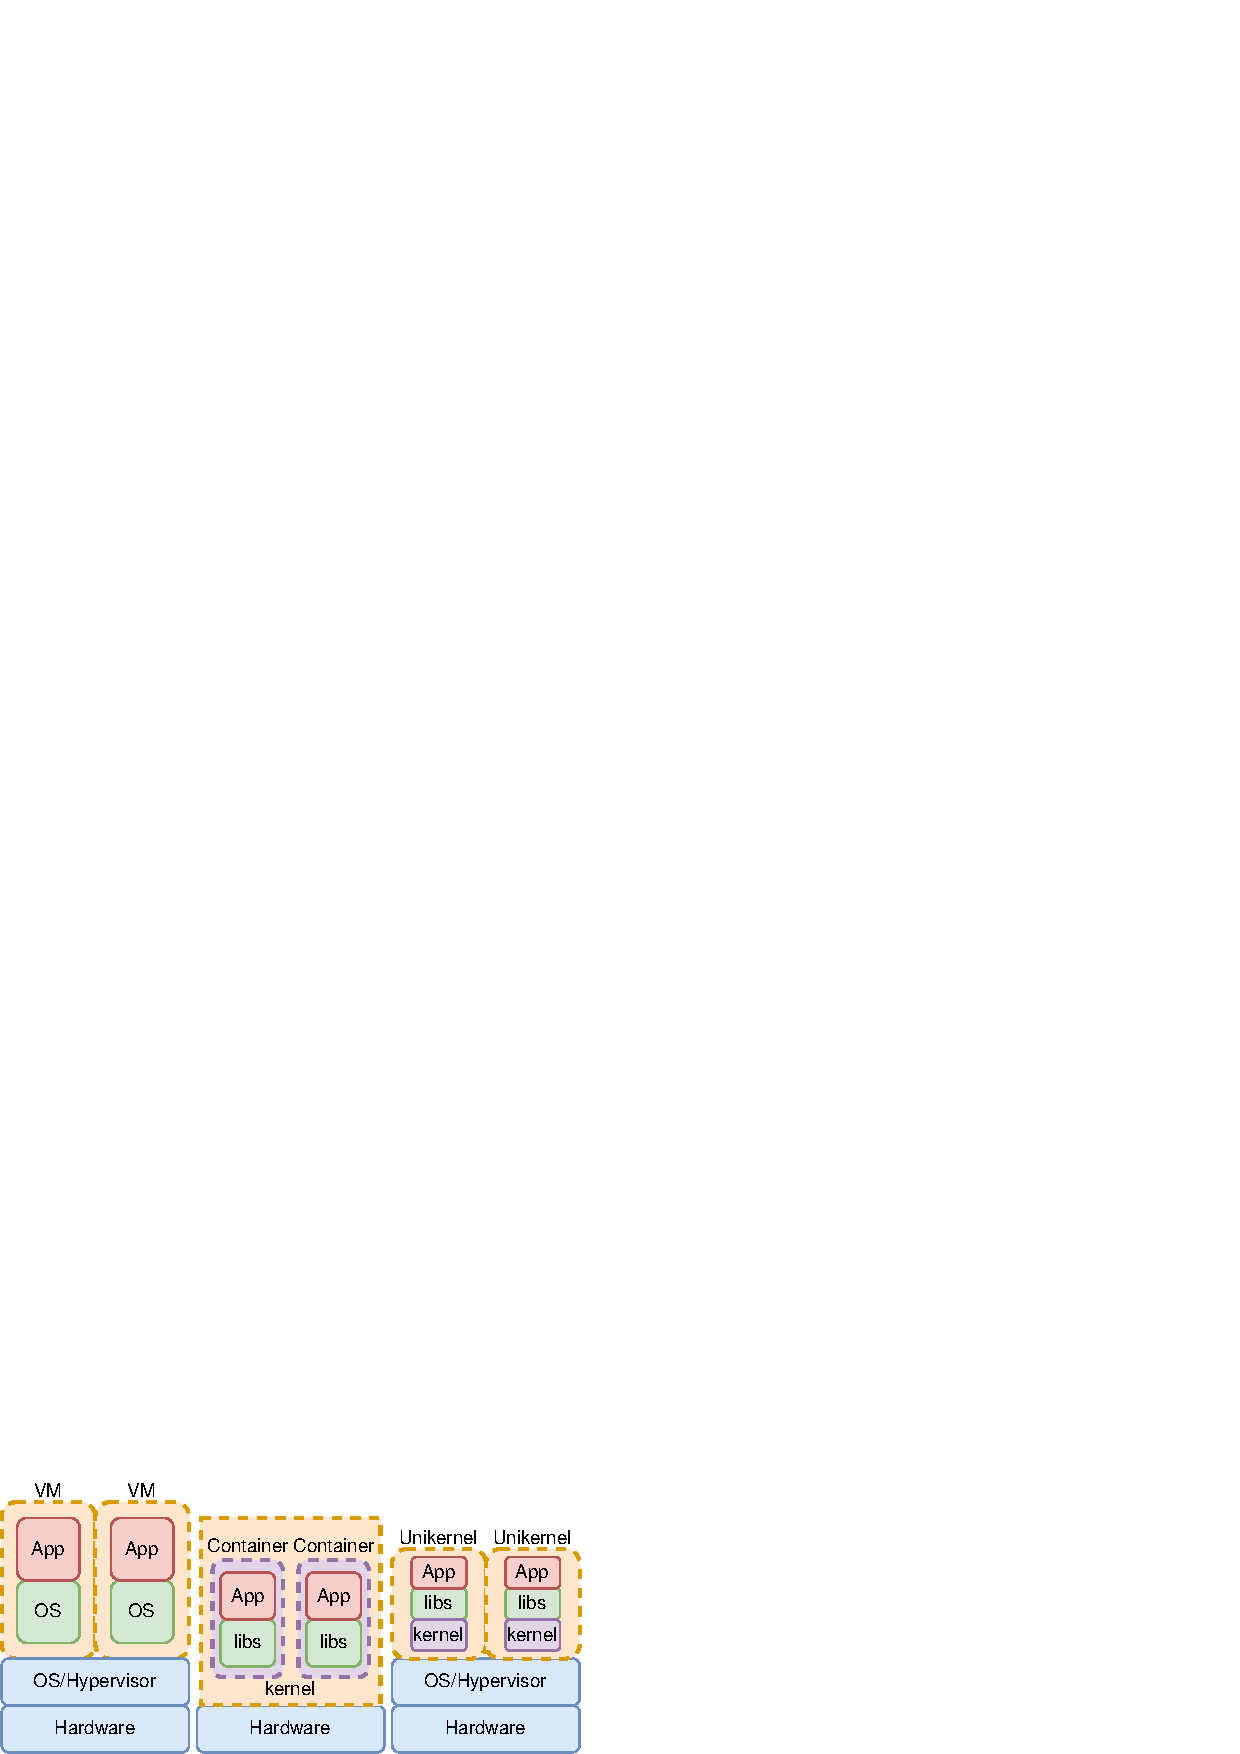
\includegraphics[scale=0.8]{images/Figure5.png}
	\end{center}
	\vspace{-0.6cm}
	\caption{Architectural differences between VMs, containers and unikernels.}
	\label{fig:fig5}
\end{figure}
%
%
\section{Deployment}\label{sec:deployment}
%
Over the years two different approuches evolved how to deploy infrastructure and applications. The difference just get more amplified, when CC and microservices get into the picture, where frequent deployment is very common. 

Here evolve new strategy to mange and deploy complicated infrastructure elements --- Infrastructure as code (IaC). In his book~\cite{wittig2018amazon} Wittig et al. describe it as a process of managing and provisioning computer data centers through machine-readable definition files, rather than physical hardware configuration or interactive configuration tools.

Deplyments in such complex environment can be separated how they handle changes on existing infrastructure or applications on:

\begin{itemize}
	\item \textbf{Mutable model}, is model where we have in place changes which mean that the parts of the existing infrastructure or applications get updated or changed in order to do update. In place change can produce few problems: $(1)$ more risk, beacause in place change my not finish completly which put our infrastructure or the application in possible bad state. This is esspecially probem, if we have a lot of services and multiple copies of the same service. Possibility that our system is not on, is a lot higher, $(2)$ high complexity, this is direct implicatoin of previous feature. Since out change might not get fully done, we can't give guarantis that our infrastructure or applicatoin is transitioned from one version to the another --- change is not \textbf{descrete}, but \textbf{continues} since we might end up in some state in between where we are now and where we want to be.
	\item \textbf{Immutable model}, is model where we do not do any in place changes on existing infrastructure or application whatsoever. In this model, we replace it complety with new version that is updated or changed compared to previous version. Previous version get discarded in favour of new version. Compared to the previous model, immutable deployment have: $(1)$ less risk, since we do not change existing infrastructure or the applicatoin but we start new one with and shut down previous one. This is important esspecially in DS where everyting can fail at any tome, $(2)$ previous property reduce complexity of mutable deployment model. This is direct implicatoin of previous feature, since we shut down and fully replace previous version with new one we get \textbf{descrete} version change and atomic deployment with dafer deployments with fast rollback and recovery processes. On the other hand, this process requre more resources~\ref{Helland16}, since both hersions must be present on the node in order to this process is done. Second problem is data that is used by the app, we should not lost the data that app is generated. If we externalize data than this problems is resolved. We should not rely on local storage, but store that data elsewhere, esspecially when the parts of the system are volatile and changed often. Key adventage of this approuch, is avoiding downtime experienced by the end user when new features are released.
\end{itemize}

Figure~\ref{fig:fig12} summaraze difference bewteen prevous infrastructure deplyment models.

\begin{figure}[H]
	\begin{center}
		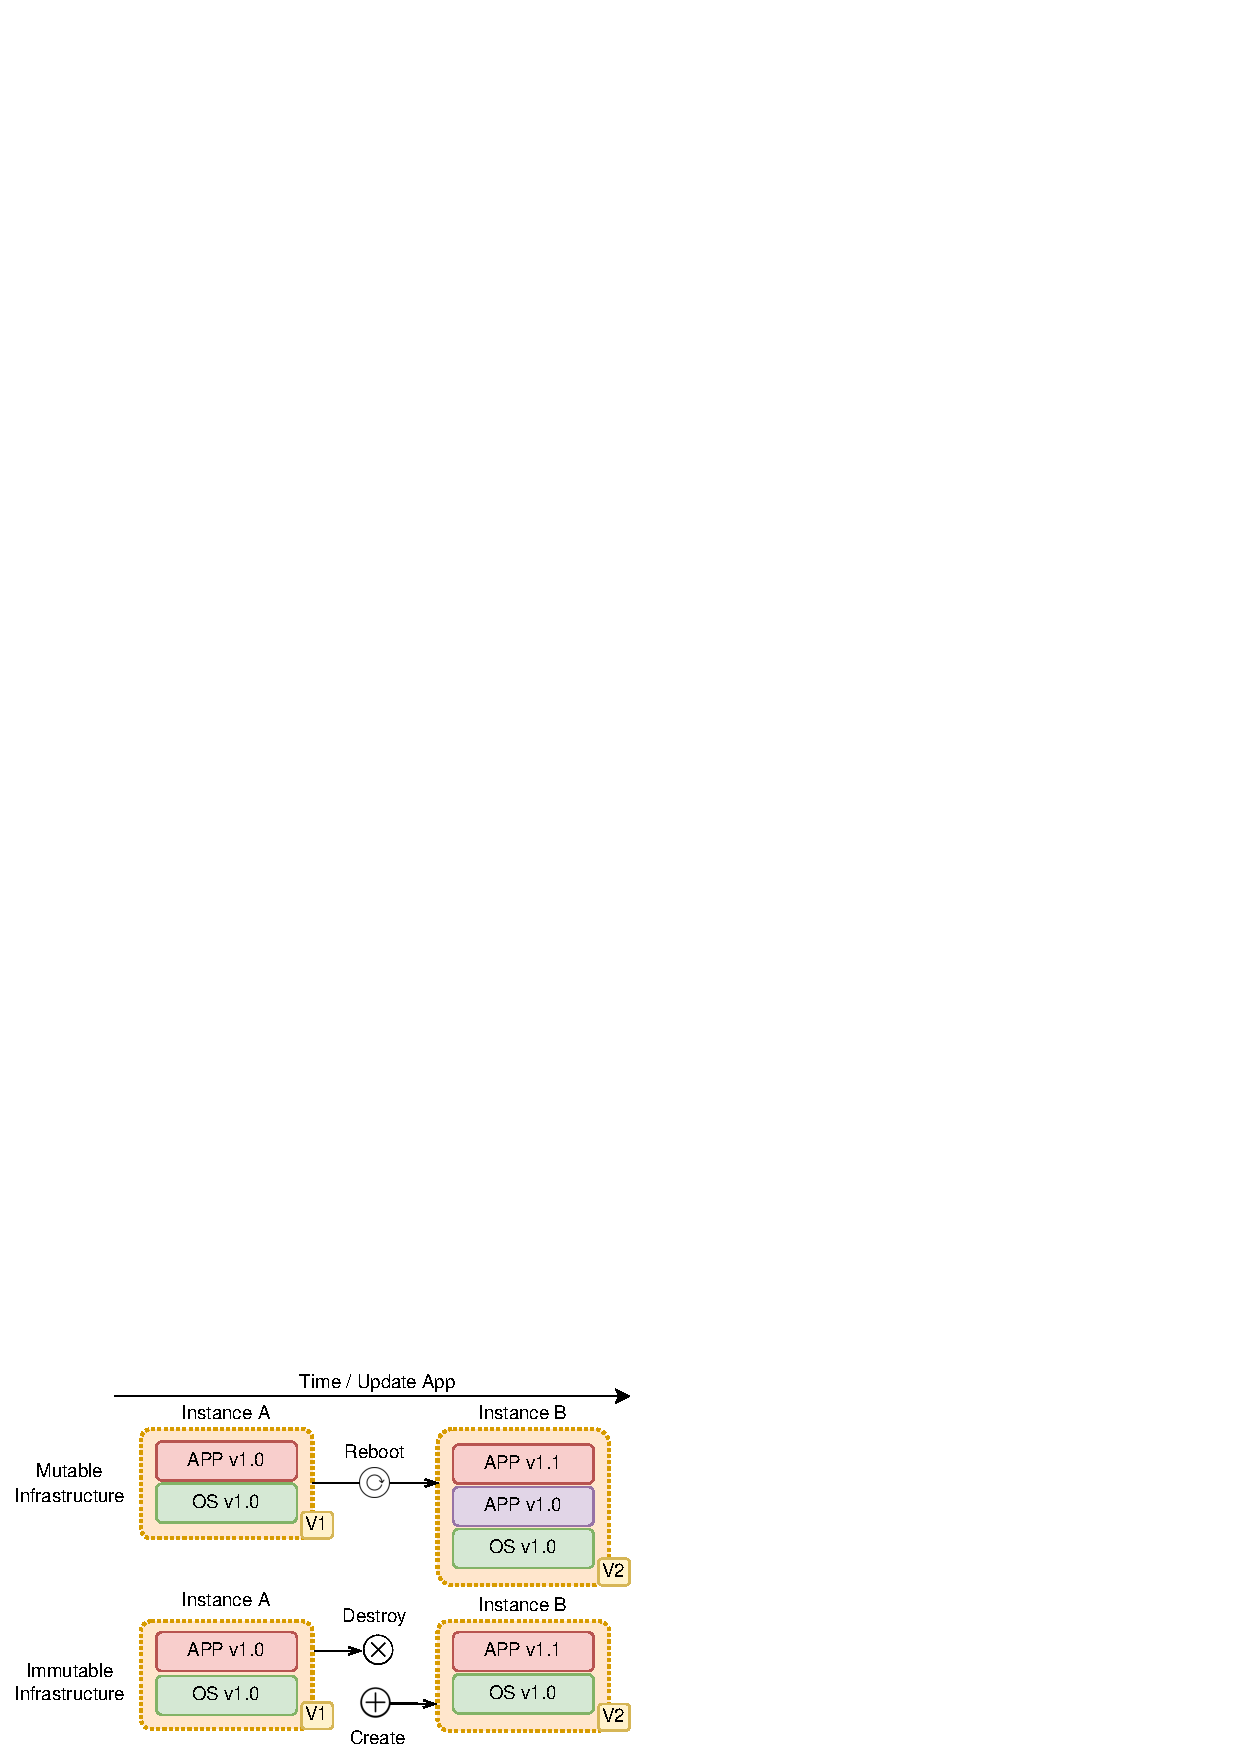
\includegraphics[scale=0.7]{images/Figure12.png}
	\end{center}
	\vspace{-0.6cm}
	\caption{Difference bewteen mutable and immutable deplyment models}
	\label{fig:fig12}
\end{figure}

Immutability is a simple concept to understand, and simplify a lot esspecially in DS~\cite{Helland16}. Write down some data, and ensure that it never changes. It can never be modified, updated, or deleted~\cite{perry2020art}. When this is combined with premisse that we can avoid downtime esspecially in complex DS, it is clear why immutable model is gainign more and more popularity (esspecially with arival of containers). Immutable infrastructure deployment offer few models how to deploy change on the services, even in production to test it, or switch to whole new version. These strategeis include:

\begin{itemize}
	\item \textbf{Blue-Green deployment}, this strategy require two separate environemnts: $(1)$ \textit{Blue} current running version, and $(2)$ \textit{Green} is the new version that needs to be deployed. When we are satisfied that the green version is working properly, we can gradually reroute the traffic from the old environment to the new environment for example by modifying DNS. This strategy offers near zero downtime.
	\item \textbf{Canary update} is the strategy where we do direct a small number of requests to the new version --- the canary. If we are satisfied with the change, we can continue to increase number of requests and monitor how service is working with increasing load, monitor for erros etc.
	\item \textbf{Rolling update} streategy update large environments a few nodes at a time. The setup is similar to blue-green deployment, but here we have single environment. With this strategy, new version gradually replaces the old one. But this is not the only benefit. If for whatever reason, new verrsion is not working properly on larger amount of nodes, we can always do rolling back to previous version.
\end{itemize}

With mutable infrastructure these strategies would be hard to implement, and maybe it is not possible at all. 

Beside infrastructure deployemnt, there is another side that we must consider, and that is how describe these deployments. Here we can consider two different strategies:
\begin{itemize}
	\item \textbf{Imperative}, with this option users have to write code or specific instructions step by step what specific tool need to do in order that application or infrastrucgure is properly setup. In this approuch we have a \textit{smart} user who describe \textit{dumb} machine what is needed to be done and in what order to achieve desired state.
	\item \textbf{Declarative}, with this option user have to describe end state or what is his desired state, and tool needs to figure out the way how to do this. Here we have \textit{smart} system that will found a way how to achieve desired state, and we have user who\textit{do not care} in what order actions need to be done --- that is what system needs to do. User do not need to worry about timing, this simplify whole process and code always represents the latest state. With this type of deployment, we can offer users two different models: $(1)$ use existing formats that are user familiar with like JSON, YAML, XML etc., or $(2)$ create new domain specific language that users need to learn, but we might be able to optimaze description.
\end{itemize}

With introduction of \textit{LinuxKit}, we can create Linux subsystems based around containers, that  are very secure. With linuxkit, every purt of the Linux subsystem is running inside container, so we can assemble a Linux subsystem with services that are needed. As a result, systems created with LinuxKit have a smaller attack surface~\cite{abs-1802-10375} than general purpose systems. This is important from security point of view, but also from infrastructure deployment because we can compose specific OS based around containers that we need for different purpose. And we can update, change and adopt these OS for every machine or purpose we need.

Deployment is based around changeint parts of the OS, and his services that are running inside containers. As a result, everything can be removed or replaced. It's highly portable and can work on desktops, servers, IoT, mainframes, bare metal, and virtualized systems.
%
%
\section{Concurency and parallelism}\label{sec:concurency_parallelism}
%
People usually confuse these two concepts. Even they looks similar, they are different way of doing things. In his talk Rob Pike~\cite{Pike} give great explanation and examples on this topic. In this toke he give great deffinitions of these concepts like:

\begin{itemize}
	\item \textbf{Concurrency} is composition of independently executing things. Concurrency is about dealing with a lot of things at once.
	\item \textbf{Parallelism} is simultaneous execution of multiple things. Parallelism is about doing a lot of things at once. 
\end{itemize}

These things are important, esspecially when building applications and systems that should achieve very high throughput. We must build them with a good structure and a good concurrency model. These features enables possible parallelism, but with communication~\cite{Pike}. These ideas are based on Tony Hoare work of Communicating Sequential Processes (CSP)~\cite{Hoare78}.

\subsection{Actor model}\label{sec:actor_model}
%
In actor model, the main idea is based around \textbf{actors} which are small concurrent code, that communicate independently by sending messages, removing the need for lock-based synchronization~\cite{Hewitt}. This model propose similar idea like Tony Hoare in his work with CSP~\cite{Hoare78}, and actors are oftten confused with CSP. Table~\ref{tab:table6} give differences between actor model and CSP.

\begin{table}[h!]
	\begin{center}
		\begin{tabular}{l|l|l}
			\textbf{Feature} & \textbf{CSP} & \textbf{Actor model}\\
			\hline
			\textbf{Fault tolerance} & Distributed Queue & Hierarchy of supervisors \\
			\textbf{Process identity} & Anonymus & Concrete \\
			\textbf{Composition} & NA & Applicable \\
			\textbf{Communication} & Queue & Direct \\
			\textbf{Message passing} & Sync & Async\\
		\end{tabular}
	\end{center}
	\vspace{-0.5cm}
	\caption{Ddifferences between actor model and CSP.}
	\label{tab:table6}
\end{table}

Actors do not share memory, and they are isolated by nature. Actor can create another actor/s and even watch on them in case they stop unexpectedly. And when an actor finished its job, and he is not needed anymore, it disappears. These actors can create complicated networks that are easy to understand, model and reason about and everything is based on a simple massage passing mechanism. 

Every actor have a designated message box. When a message arrives, actor will test message type and do job acording to message type he received. In this way we are not dependent of lock-based synchronization that can be hard to understand, and it can cause serious problems.

Actor model is fault tolerant by design. It support crush to happend, because there is a \say{self heal} mechanism that will monitor actor/s, and when crash happend it will try to apply some strategy, in most cases just restart actor, but other strategies could be applied. This philosophy is really usefull, because it is hard to think about every single failure option.
%
%
\section{Motivation and Problem Statement}\label{sec:problem_statement}
%
In~\cite{GreenbergHMP09} Greenberg et al. point out that micro data-centers (MDCs) are used primarily as nodes in content distribution networks and other \say{embarrassingly distributed} applications.

One size never fits all, so the cloud should not be our final computing shift. Various models presented in~\ref{sec:mobile_computing}, show possibility that computing could be done closer to the data source, to lower the latency for its clients by contacting the cloud only when needed, while heavy computation remains in the cloud because of resource availability. Send to the cloud only information that is crucial for other services or applications~\cite{inproceedingsSimic1}. Not ingest everything as the standard cloud model proposes.

MDCs with a zone-based server organization is a good starting point for building EC as a service, but we need a more available and resilient system with less latency. EC originates from P2P systems~\cite{LopezMEDHIBFR15} as sugested by L{\'{o}}pez et al., but expands it into new directions and blends it with the CC. But, infrastructure deployment will not happen until the process is trivial~\cite{SatyanarayananBCD09}. Going to every node is tedious and time consuming. Especially when geo-distribution is taken into consideration.

A well defined system could be offered as a service, like any other resource in the CC. We can offer it to researchers and developers to create new human-centered applications. If we need more resources on one side, we can take from one pool of resources and move to another one.
But on the other hand, some CC providers might choose to embed it into their own existing system, hiding unnecessary complexity, behind some communication interface or proposed application model.

The idea of small servers with heterogeneous compute, storage, and network resources, raise interesting research idea and motivation for this thesis. Taking advantage of resources organized locally as micro clouds, community clouds, or edge clouds~\cite{RydenOCW14} suggested by Ryden et al., to help power-hungry servers reduce traffic~\cite{HirschMZ18}. Contact the cloud only when needed~\cite{inproceedingsSimic1}. Send to the cloud only information that is crucial for other services or applications. Not ingest everything as the standard CC model proposes.

To achieve such behavior, dynamic resource management, and device management is essential. We must perceive available resources, configuration, and utilization~\cite{GubbiBMP13, WangZZWYW17}. Traditional DCs is a well organized and connected system. On the other hand, these MDCs consist of various devices, including ones presented in~\ref{sec:mobile_computing} that are not~\cite{JiangCGZW19}. This idea, brings us to the problem this thesis address.

EC and MDCs models lack dynamic geo-organization, well defined native applications model, and clear separation of concerns. As such they cannot be offered as a service to the users. They usually exist independently from one another, scattered without communication between them, offered by providers who mostly lock users in their own ecosystem. Co-located edge nodes should be organized locally, making the whole system and applications more available and reliable, but also extending resources beyond the single node or group of nodes, maintaining good performance to build servers and clusters~\cite{ArocaG12}.

This cloud extension deepens and strengthens our understanding of the CC as a whole. With the separation of concerns setup, EC native applications model, and a unified node organization, we are moving towards the idea of EC as a service. 

Based on this, we define the problem through the following research questions three segments:

\begin{enumerate}[start=1,label={(\bfseries \arabic*)}]
	\item \textit{Can we organize geo-distributed edge nodes in a similar way to the cloud, adopted for the different  environment, with clear separation of concerns and familiar applications model for users.}
	\item \textit{Can we offer these organized nodes as a service to the developers and researchers for new human-centered applications, based on the cloud pay as you go model?}
	\item \textit{Can we make model in such a way that is formaly correct, easy to extend, understand and reason about?}
\end{enumerate}

This cloud-like extension makes the whole system and applications more available and reliable, but also extends resources beyond the single node. Satyanarayanan et al. in ~\cite{SatyanarayananK19} show that MDCs can serve as firewalls, while Simi\' c et al., in~\cite{inproceedingsSimic1} use similar idea as pre-processing tier. At the same time, users are getting a unique ability to dynamically and selectively control the information sent to the cloud. Years after its inception, EC is no longer just an idea~\cite{SatyanarayananK19} but a must-have tool for novel applications to come.
%
%
\section{Research Hypotheses, and Goals}\label{sec:research_hyphotesis_and_golas}
%
Based on reserach questions and motivation presented in~\ref{sec:problem_statement}, we derive the hypotheses around which the thesis is based. It can be summarized as follows:

\begin{enumerate}[start=1,label={(\bfseries \arabic*)}]
	\item \textbf{Hypothesis:} \textit{It is possible to organize EC nodes in a standard way based on cloud architecture, with adaptation for an EC geo-distributed environment. Give users the ability to organize nodes in the best possible way in some geographic areas to serve only the local population in near proximity.}
	\item \textbf{Hypothesis:} \textit{It is possible to offer it to researchers and developers to create new human-centered applications. If we need more resources on one side, we can take from one pool of resources and move to another one, or organize them any other way needed.}
	\item \textbf{Hypothesis:} \textit{It is possible to present clear separation of concerns for the future EC as a service model, and establish a well-organized system where every part has an intuitive role.} 
	\item \textbf{Hypothesis:} \textit{It is possible to present unified model that supports heterogeneous EC nodes, with a set of technical requirements that nodes must fulfil, if they want to join the system.}
	\item \textbf{Hypothesis:} \textit{It is possible to present a clear application model so that users can use full potential of newly created infrastructure.}
\end{enumerate}

From the previously defined hypotheses, we can derive the primary goals of this thesis, where the expected results include:

\begin{enumerate}[start=1,label={(\bfseries \arabic*)}]
	\item \textit{The construction of a model with a clear separation of concerns for the model influenced by cloud organization, with adaptations for a different environment. With a model for EC applications utilizing these adaptations. This addresses the first research question, and is the topic of Chapter~\ref{chapter:Micro_clouds}.}
	\item \textit{The constructed model is more available, resilient with less latency, and as such it can be offered to the general public as a service like any other service in the cloud. This addresses the second research question, and is the topic of Chapter~\ref{chapter:Micro_clouds}.}
	\item \textit{The constructed model is described formaly well, using solid mathematical theory, but also easy to extend both formaly and technicaly, easy to understand and reason about. This addresses the third research question, and is the topic of Chapter~\ref{chapter:Micro_clouds}.}
\end{enumerate}
%
%
\section{Structure of the thesis}\label{sec:structure_of_thesis}
%
Throughout this introductory Chapter, we defined the motication for out work with problems that this thesis addresses and presented the necessary background informations and areas to support our work. Here we outline the rest of the thesis.

Chapter~\ref{chapter:Review} presents the literature review, where we examine different aspects of existing systems and methods important for the thesis. We analyze existing nodes organizational abilities in both industry and academia frameworks and solutions to address our first research question. We further exemine platform models from industry and academia tools and frameworks to address our second research question. And last but not least, we examine current strategies to offload tasks from the cloud. All three parts address our third research question.

Chapter~\ref{chapter:Micro_clouds} details our model, how it is related to other research and where it connects to other existing models and solutions. We further describe our solution as well as protocols requried for such sysrtem to be implemented foramly. We give examples of how exisintg infrastructure could be used, as well as familiar application model for developers. 

Chapter~\ref{chapter:Implementation} present implementation details of an framework developed to test hypotheses defined earlier in this chapter, but also model and foramly defined protocols defined in~\ref{chapter:Micro_clouds}. This chapter also show results after conducting experiments, current limitations of implemented system, and possible applications that could benefit from such system.

Chapter~\ref{chapter:Conclusion} concludes our work and presents opportunities for further research and development.
%
%
%!TEX root =  main.tex
\chapter{A calculus for confidential name passing}\label{chapter:Cpi}



In this chapter, we present the $C_\pi$-calculus, which is a fragment of the $\pi$-calculus~\cite{DBLP:books/daglib/0098267, DBLP:journals/iandc/MilnerPW92a, DBLP:journals/iandc/MilnerPW92b,  pi_calculus}.  
We start by a small introduction on process algebras. %, closely related to our work.

As in the $\pi$-calculus, the building blocks of the $C_\pi$ language are \emph{processes}. 
A process represents an entity that can synchronize with other processes through communication links (channels) that they share.
%The execution of a process is performed by means of channel actions conducted by threads. 
%These actions can be concurrent, and two threads can synchronize their actions. 
Some of the first and well-known process models are a Calculus of Communicating Systems ($CCS$)~\cite{DBLP:books/sp/Milner80} and Communicating Sequential Processes ($CSP$)~\cite{DBLP:books/ph/Hoare85}. 
The latter has influenced the design of Google's \emph{Go} programming language. 
See~\cite{DBLP:journals/tcs/Baeten05} for a more comprehensive overview of the history of process algebras.

The $CCS$-calculus models concurrent systems formally by introducing the notions of parallel composition, synchronization of input and output action on the same name, the private names and the choice. The choice operator is not considered throughout this thesis, and hence we will not mention its interpretation nor its properties.
For instance, a $CCS$ process $\mathit{Alice} \parop \mathit{Bob}$ represents that $\mathit{Alice}$ and $\mathit{Bob}$ are simultaneously active processes. Furthermore, these processes can synchronize via shared name. For instance, in process
\[
\overline{\mathit{chn}}.\mathit{Alice} \parop {\mathit{chn}}.\mathit{Bob}
\] 
process $\overline{\mathit{chn}}.\mathit{Alice}$ can synchronize the output action on name $\mathit{chn}$ with the input action of process ${\mathit{chn}}.\mathit{Bob}$, since both are active in parallel. In that case, the process reduces to $\mathit{Alice} \parop \mathit{Bob}$.

In $CCS$ a name can be specified as private. In process 
\[
(\rest{\mathit{session}}\mathit{Alice}) \parop \mathit{Bob}
\]
name $\mathit{session}$ is known only to $\mathit{Alice}$ and can be used only internally, while $\mathit{Bob}$ cannot acquire the name. What $CCS$ fails to capture directly is name mobility.

The $\pi$-calculus takes as its basis $CCS$, but it extends it in an important way by allowing name mobility.  Namely, processes now can, while synchronizing their actions (via communication channels), transmit names of channels. This model has also influenced the design of several programming languages~\cite{ DBLP:conf/afp/FournetFMS02, DBLP:journals/entcs/MeredithR05,  DBLP:conf/birthday/PierceT00, DBLP:journals/jfp/SewellLWNAHV07,DBLP:conf/wecwis/ThiagarajanSPB02,DBLP:conf/birthday/WelchB04}. For example, in the $\pi$-calculus we may specify 
\[
\send{\mathit{chn}}\role\msg{\mathit{session}}.\mathit{Alice} \parop \receive{\mathit{chn}}\role\msg\NX.\mathit{Bob}
\]
where the left process can send channel name $\mathit{session}$ on channel $\mathit{chn}$, the right process can receive a name on the same channel and replace the placeholder name $\NX$ in $\mathit{Bob}$ with the received name. 
Another important aspect is that a $\pi$ process can share a private communication channel with other processes via synchronization, establishing private connections. 
This is the last ingredient needed to represent the scenario given in the Introduction, as we may now write
\[
(\rest{\mathit{session}}\send{\mathit{chn}}\role\msg{\mathit{session}}.\mathit{Alice}) \parop \receive{\mathit{chn}}\role\mgs{\NX}.\send{\mathit{forward}}\role\msg\NX.\mathit{Bob}'
\]
where the channel $\mathit{session}$ is privately held by the left process. After the synchronization, the above configuration evolves to 
\[
\rest{\mathit{session}}(\mathit{Alice} \parop \send{\mathit{forward}}\role\msg{\mathit{session}}.\mathit{Bob}'')
\]
where private channel $\mathit{session}$ is received in the right process (i.e., $\mathit{Bob}''$ represents the process derived from $\mathit{Bob}'$ by replacing each occurrence of name $\NX$ with name $\mathit{session}$), hence enlarging the scope of the name. Assuming there is a third party active,
\[
\rest{\mathit{session}}(\mathit{Alice} \parop \send{\mathit{forward}}\role\msg{\mathit{session}}.\mathit{Bob}'') \parop \receive{\mathit{forward}}\role\msg\NY.\mathit{Carol}
\]
 the process comprehending $\mathit{Bob}''$ can forward received name $\mathit{session}$ to the third party on channel $\mathit{forward}$ without a need to notify $\mathit{Alice}$, hence potentially compromising the privacy of $\mathit{Alice}$ (cf. Section~\ref{sec:intro_sharing_control}). 

%Both features add considerably to the expressive power of the $\pi$-calculus. 

The subject of this section, the $C_\pi$-calculus, allows reasoning on confidentiality in a fragment of the $\pi$-calculus. 
By restricting forwarding in a way that channel name once received by a process cannot be later sent by the same process, we gain a suitable abstraction level to reason on, e.g., groups~\cite{cardelli05} and name hiding~\cite{Giunti}, directly in the $C_\pi$ without additional language constructs. Since we are dealing only with a fragment of the $\pi$-calculus rather than with its extension, our model can reuse all the theory already developed for the $\pi$.

Extensive theoretical research conducted in the past is directly connected to the $\pi$-calculus in many ways. 
Many of these works extend the $\pi$-calculus syntax by variety of constructs so as to gain a suitable abstraction level to reason about, e.g.,  
polyadic communications~\cite{DBLP:journals/njc/CarboneM03, DBLP:conf/concur/Milner92}, 
higher-order communication~\cite{DBLP:conf/csl/Milner93}, 
distributed systems~\cite{DBLP:books/daglib/0018113}, and many others, including 
security and privacy~\cite{appliedpi,spi,cardelli05,pigroups,Giunti,hennessy05}.
In contrast, some of the research exploits restricting the syntax of the $\pi$-calculus to reason on asynchronous communications~\cite{boudol:inria-00076939, DBLP:conf/ecoop/HondaT91}, internal mobility~\cite{DBLP:journals/tcs/Sangiorgi96a}, and locality~\cite{merro04}.



\paragraph{Overview of the chapter.}
The syntax of the process model is presented in Section~\ref{sec:Cpi-syntax}. 
The action semantics is presented in Section~\ref{sec:Cpi-semantics}, followed by an investigation of some basic properties together with the definition of the non-forwarding property in Section~\ref{sec:Cpi_properties_of_lts}. The reduction semantics is briefly introduced in Section~\ref{sec:Cpi-reduction-semantics}. 
Section~\ref{sec:Cpi-bisimilarity} presents a behavioral equivalence (strong bisimilarity) and a property called closed domains for channels, capturing that closing the scope of a channel can be represented directly in $C_\pi$. 
Section~\ref{sec:strong_barbed_equivalence} briefly presents another behavioral equivalence, the strong barbed equivalence relation, and Section~\ref{sec:the_non-forwarding_of_pi_processes} gives a method for identifying non-forwarding $\pi$ processes.
In Section~\ref{sec:examples} we present some interesting scenarios modeled in $C_\pi$, such as  authentication schemes (Section~\ref{sec:authentication}), closing the domain for channels (Section~\ref{sec:groups}), and open-ended groups (Section~\ref{sec:open-ended-groups}). Section~\ref{sec:encoding} presents an encoding from the $\pi$-calculus into the $C_\pi$-calculus and the operational correspondence result that validates the encoding and informs on the expressive power of $C_\pi$. 



%
\begin{table}[t]
\[
\displaystyle
\begin{array}[t]{rcl@{\qquad\qquad\qquad}r}
 \pi & ::= & 								 &   \emph{Prefixes}\\
     &        & \send\NA\role\msg\NK    	 &   \text{output}\\
     & \parop & \receive\NA\role\msg{x} 	 &   \text{input}\\
     & \parop & \match\NA\role\msg\NB\pi     &   \text{matching}\\
     &        &								 &   \\
  \PP & ::= & 								 &	 \emph{Process terms}\\
     &        & \inact 						 &   \text{termination}\\
     & \parop & \pi.\PP  					 &   \text{prefix}\\
     & \parop & \PP\parop\PP 				 &   \text{parallel composition}\\
     & \parop & \rest\NK \PP  				 &   \text{name restriction}\\
     & \parop & \rep\PP 					 &   \text{replication}\\
\end{array}
\]
\caption{\label{tab:Cpi_syntax} Syntax of $C_\pi$}
\end{table}
%




\section{Syntax}\label{sec:Cpi-syntax} 

In this section, we introduce the language of the $C_\pi$-calculus. 
As we have noted, the building blocks of our language are processes, 
and processes may communicate using names. 
The names themselves are an abstraction for communication links. Communication links are modeled as named communication channels that can connect two or more processes. 

In $C_\pi$, we distinguish \emph{variable} and \emph{channel} names by introducing two disjoint sets for each kind. 
We use $\Chn$ to denote the set of channel names, ranged over by $\NK, \NL, \NM, \ldots$, and $\Var$ to 
denote the set of variable names, ranged over by $\NX, \NY, \NZ, \ldots$ 
The union of the two sets is denoted by $\N$, and we let $\NA, \NB, \NC, \ldots$ range over $\N$. 
The use of each of the sets is explained below when language constructs are introduced.


The syntax of the language is given in Table~\ref{tab:Cpi_syntax}. Notice that we do not consider the sum operator~\cite{pi_calculus} since our goal is to study confidentiality in a minimal setting, but we believe the sum can be added following expected lines.
The first part of the table introduces the prefixes, used in the definition of three types of processes: 
%
\begin{itemize}
\item The output prefix $\send\NA\role\msg\NK.\PP$ describes an action in which the object, channel name $\NK$, is sent on the subject, name $\NA$,  after which the process evolves to $\PP$. 
Notice that only a channel name, i.e., a name from set $\Chn$, can be the object of an output action. 
This is the only difference with respect to the $\pi$-calculus, where the name of a variable can also appear as the object of an output action. 
The subject of an output action can be either a channel or variable name, like in the $\pi$-calculus. 
Hence, received names can be used to communicate but cannot be communicated. For example, process $\send\NB\role\msg\NK.\inact$ can send $\NK$ on $\NB$ and evolve to $\inact$.
%
\item The input prefix $\receive\NA\role\msg\NX.\PP$ describes an action in which a name is received on the subject name $\NA$. The received name is substituted in the continuation process $\PP$ for a variable name $\NX$, and the original process evolves to the term resulting from this substitution. Here, $\NX$, also called a placeholder, is bound in process $\PP$ (see Definition~\ref{def:Cpi_bound_names}). 
For example, process $\receive\NA\role\msg\NX.\send\NX\role\msg\NK.\inact$ can receive a name on $\NA$ and substitute $\NX$ by it in the continuation. 
Assuming the received name is $\NB$, the above process evolves to $\send\NB\role\msg\NK.\inact$. 
Notice that the object of an input can only be a variable name, i.e., name from set $\Var$. 
Hence, process as $\receive\NA\role\msg\NX.\send\NK\role\msg\NX.\inact$ excluded by the $C_\pi$ syntax is a $\pi$ process.
\item The match prefix $\match\NA\role\msg\NB\pi.\PP$ activates the action prescribed by prefix $\pi.\PP$ only if $\NA=\NB$ and it blocks the action otherwise. For example, process 
$\receive\NA\role\msg\NX.\match\NX\role\msg\NB\send\NX\role\msg\NK.\inact$ 
receives a name on $\NA$, then either: it sends $\NK$ on $\NB$ if the name received is $\NB$; else if the received name is not $\NB$ it performs no further actions.
\end{itemize}

We comment the rest of the process constructs:
\begin{itemize}
\item The termination $\inact$ denotes the process that exhibits no actions. 
Notice that we have used it in the examples above to signal when a thread has performed all its 
actions.
%
\item The parallel composition $\PP \parop \PP$ denotes that two processes are simultaneously active, and possibly can synchronize their actions. 
For example, in $\send\NA\role\msg\NK.\inact \parop \receive\NA\role\msg\NX.\send\NX\role\msg\NL.\inact$ 
the left thread can synchronize the output action with the input action of the right thread, and   
%in which case the above configuration evolves to $\inact \parop \send\NK\role\msg\NL.\inact$. 
%Notice also that the synchronization does not have to take place and that above configuration 
can also exhibit any of the individual actions of the two threads.
%
\item The name restriction $\rest\NK\PP$ denotes the creation of a new (channel) name $\NK$, 
known only to process $\PP$. 
Channel $\NK$ can be used as a private medium for communications of the components of process $\PP$. 
For example, process $\rest\NK(\send\NK\role\msg\NL.\inact \parop \receive\NK\role\msg\NX.\inact)$ 
can use channel $\NK$ for synchronization of the two threads but cannot interact with other processes along channel $\NK$.
On the other hand, the restricted channel can be shared with other processes if it is communicated in a message. 
The explanation of sharing restricted names and its interplay with confidentiality in $C_\pi$ can be found in  Section~\ref{sec:Cpi-semantics}, Section~\ref{sec:Cpi-bisimilarity} and Section~\ref{sec:examples}.
%
\item The replication $\rep\PP$ denotes a process with potentially infinite behavior. 
Informally, $\rep\PP$ can be seen as an infinite parallel composition of the copies of process 
$\PP$, i.e., $\PP\parop\PP\parop\ldots$. 
For example, process $\rep\send\NA\role\msg\NK.\PQ$ can send $\NK$ on $\NA$ and activate 
the original process in parallel. %, evolving to  $\PQ \parop \rep\send\NA\role\msg\NK.\PQ$.
\end{itemize}


We name the operators' precedence from highest to lowest: prefixes, name restriction, replication, and parallel 
composition. 
For example, the above process 
$\send\NA\role\msg\NK.\inact \parop \receive\NA\role\msg\NX.\send\NX\role\msg\NL.\inact$ stands for 
$(\send\NA\role\msg\NK.\inact) \parop (\receive\NA\role\msg\NX.(\send\NX\role\msg\NL.\inact))$, 
%process $\rep\send\NA\role\msg\NK.\PP$ stands for $\rep(\send\NA\role\msg\NK.\PP)$, 
and $\rest\NK\PP \parop \PQ$ stands for $(\rest\NK\PP) \parop \PQ$.


We denote with $\n\PP$ the set of all names (channels and variables from $\N$) appearing in the process $\PP$. 
Some of these names are said to be \emph{free}, while the rest are called \emph{bound}. 

\begin{definition}[Free and bound names]\label{def:Cpi_bound_names}
For any $C_\pi$ process the set of free names $\fn\PP$ and the set of bound names $\bn\PP$ are defined  as follows.
\[
\begin{array}{rcl}
\fn{\inact} & = & \emptyset\\
\fn{\send\NA\role\msg\NK.\PP} & = & \{\NA, \NK\} \cup \fn\PP\\
\fn{\receive\NA\role\msg\NX.\PP} & = & \{\NA\} \cup (\fn\PP\setminus\{\NX\})\\
\fn{\match\NA\role\msg\NB\pi.\PP} & = &  \{\NA, \NB\} \cup \fn{\pi.\PP}\\
\fn{\PP \parop\PQ} & = & \fn\PP \cup \fn\PQ\\
\fn{\rest\NK\PP} & = & \fn\PP\setminus \{\NK\}\\
\fn{\rep\PP} & = & \fn\PP
\end{array}
\qquad
\begin{array}{rcl}
\bn{\inact} & = & \emptyset\\
\bn{\send\NA\role\msg\NK.\PP} & = & \bn\PP\\
\bn{\receive\NA\role\msg\NX.\PP} & = & \{\NX\} \cup \bn\PP\\
\bn{\match\NA\role\msg\NB\pi.\PP} & = &  \bn{\pi.\PP}\\
\bn{\PP \parop\PQ} & = & \bn\PP \cup \bn\PQ\\
\bn{\rest\NK\PP} & = & \{\NK\} \cup \bn\PP\\
\bn{\rep\PP} & = & \bn\PP
\end{array}
\]
\end{definition}

Notice that in $\rest\NK \PP$ and $\receive\NA\role\msg\NX.\PP$ the channel 
$\NK$ and variable $\NX$ are bound and that these are the only operators that bind names. 
In these two cases, we say that $\NK$ and $\NX$ are binding 
with \emph{scope} $\PP$. 
The scope of a bound name determines the process which is the only one that knows the name.
Notice that $\fn\PP=\n\PP\setminus\bn\PP$. 
For free names, the scope is not predefined since free names may be known by other processes.
We also identify a set of free channels appearing as objects of output prefixes in a process, so as to be able to talk about names a process can send.
%
\begin{definition}[Free output object names]\label{def:Cpi_fo}
For any $C_\pi$ process $\PP$, the set of free output object names $\fo\PP$ is defined as follows.
\[
\begin{array}{rcl}
\fo{\inact} & = & \emptyset\\
\fo{\send\NA\role\msg\NK.\PP} & = & \{\NK\} \cup \fo\PP\\
\fo{\receive\NA\role\msg\NX.\PP} & = &  \fo\PP\\
\fo{\match\NA\role\msg\NB\pi.\PP} & = &  \fo{\pi.\PP}\\
\fo{\PP \parop\PQ} & = & \fo\PP \cup \fo\PQ\\
\fo{\rest\NK\PP} & = & \fo\PP\setminus\{\NK\}\\
\fo{\rep\PP} & = & \fo\PP
\end{array}
\]
\end{definition}


% We have informally  the substitution of names in the example where  
%$\send\NA\role\msg\NK.\inact \parop \receive\NA\role\msg\NX.\send\NX\role\msg\NL.\inact$ 
%evolves to 
%$\inact \parop \send\NK\role\msg\NL.\inact$, 
%where $\NX$ in the continuation of the right thread has been substituted for the received name $\NK$. 
To precisely define replacements of names in processes (such as the ones described in the receive actions) we give a precise definition of the substitution.  Before that, we introduce a convention that bound names must not be mentioned by substitutions (we will come back to this point).

\begin{definition}[Substitution]\label{def:Cpi_substitutions}
A substitution is a mapping from $\N$ to $\N$ that is not the identity only on a finite subset of $\N$, and that maps $\Chn$ only to $\Chn$. We define the support of $\sigma$ to be finite set $\{\NA\;|\; \sigma{\NA}\not=\NA \}$, and the co-support of $\sigma$ to be finite set $\{\sigma(\NA) \;|\; \sigma{\NA}\not=\NA \}$. We write $\n\sigma$ for the union of the support and the co-support of $\sigma$.
If substitution $\sigma$ is applied to process $\PP$, then the resulting process $\PP\sigma$ is defined  as follows.
\[
\begin{array}{rclr}
\inact\sigma & = & \inact\\
(\send\NA\role\msg\NK.\PP)\sigma & = & \send{\sigma(\NA)}\role\msg{\sigma(\NK)}.\PP\sigma \\ %, &\text{ where } \sigma(\NK)\in\Chn \\
(\receive\NA\role\msg\NX.\PP)\sigma & = & \receive{\sigma(\NA)}\role\msg{\NX}.\PP\sigma\\ %, & \text{ where } \NX\notin\n\sigma \\
(\match\NA\role\msg\NB\pi.\PP)\sigma & = &  (\match{\sigma(\NA)}\role\msg{\sigma(\NB)}(\pi.\PP)\sigma\\
(\PP \parop\PQ)\sigma & = & \PP\sigma \parop \PQ\sigma\\
(\rest\NK\PP)\sigma & = & \rest{\NK} \PP\sigma\\ %,   & \text{ where } \NK\notin\n\sigma\\
(\rep\PP)\sigma & = & \rep\PP\sigma
\end{array}
\]
If the support of $\sigma$ is $\{\NA_1, \ldots, \NA_n\}$, and $\sigma(\NA_i)=\NB_i$, for $i=1,\ldots,n$, then instead of $\PP\sigma$ we may also write $\PP\subst{\NB_1, \ldots, \NB_n}{\NA_1, \ldots, \NA_n}$.
\end{definition}
%
For example, we have  
$(\send\NX\role\msg\NL.\inact)\subst{\NK}{\NX}=\send\NK\role\msg\NL.\inact$. 
Notice also that substitution applied on a process does not affect the bound names of the process. 
Only free names can be substituted and the convention preceding Definition~\ref{def:Cpi_substitutions} ensures that substitution does not map free names into bound names. %, as ensured by the side-conditions in the definition. 
This is required to avoid name clashes, the notion explained next.

So far, our syntax allows us to define a process in which a name may be used in distinct binding occurrences, and also to appear free elsewhere.
%which interfere with our interpretation that a bound name cannot be known outside of its scope. 
For example, we can write 
$\rest\NK\send\NA\role\msg\NK.\inact \parop \rest\NK\receive\NA\role\msg\NX.\send\NX\role\msg\NK.\inact$, 
where, the two restricted names are identified with the same $\NK$. After synchronization of the two branches, name $\NK$ from the left branch can clash with the $\NK$ in the right branch. 
In order to simplify the handling of bound names, which are to be considered distinct regardless of their identifier, we identify processes up to $\alpha$-conversion defined next.
%To avoid this type of bound name clashes we identify  processes up to $\alpha$-conversion.
%
\begin{definition}[$\alpha$-conversion]\label{def:alpha-conversion}
Processes $\PP$ and $\PQ$ are $\alpha$-convertible if we may obtain $\PQ$ from $\PP$ by a finite number of replacements of subterms $\rest\NK\PP_1$ and $\receive\NA\role\msg\NX.\PP_2$ in $\PP$ by $\rest\NL\PP_1\subst{\NL}{\NK}$ and $\receive\NA\role\msg\NY.\PP_2\subst{\NY}{\NX}$, where $\NL\notin\n{\PP_1}$ and $\NY\notin\n{\PP_2}$.
If $\PP$ and $\PQ$ are $\alpha$-convertible we write $\PP\equiv_\alpha\PQ$.
\end{definition}
%
Notice that since we identify $\alpha$-convertible processes, $\PP\equiv_\alpha \PQ$ implies $\PP=\PQ$.
We may then say that process
$\rest\NK\send\NA\role\msg\NK.\inact \parop \rest\NK\receive\NA\role\msg\NX.\send\NX\role\msg\NK.\inact$ is 
equal to 
\[
\rest\NK\send\NA\role\msg\NK.\inact \parop \rest\NM\receive\NA\role\msg\NX.\send\NX\role\msg\NM.\inact
\] 
which allows avoiding the name clash when reasoning on the synchronization.
%where $\NK$ in the right thread is renamed to $\NM$, and after the synchronization, the two bound names do not clash.

To avoid name clashes, in general, %including cases where a bound name can clash with a free name, as in process  $\rest\NK\send\NA\role\msg\NK.\inact \parop \receive\NA\role\msg\NX.\send\NX\role\msg\NK.\inact$, where in the left thread $\NK$ is bound, while in the right thread the same name appears as free,
we use a sort of Barendregt convention as adopted in the $\pi$-calculus in~\cite{pi_calculus} Convention~$1.1.7$,
which states that all free names and names of the substitutions are distinct from all bound names in any processes and substitutions under consideration. 
%Notice that this exactly matches Convention~$1.1.7.$ in~\cite{pi_calculus}. 
Furthermore, to avoid explicitly working with $\alpha$-conversion, we also assume that all bound names among themselves in any process under consideration are different. 

We remark that this treatment of bound and free names is appealing in theoretical works on the $\pi$-calculus such as ours, but when a formalization of the $\pi$-calculus in some theorem proving systems (e.g., Coq~\cite{DBLP:series/txtcs/BertotC04}, Isabelle/HOL~\cite{DBLP:books/sp/NipkowPW02}) is conducted, a more precise way of handling free and bound names is needed, like adopting de Bruijn notation of names~\cite{DEBRUIJN1972381} to the $\pi$-calculus~\cite{DBLP:conf/tphol/Gay01, DBLP:conf/tphol/Hirschkoff97,  DBLP:journals/mscs/PereraC18}.













\section{Action semantics}\label{sec:Cpi-semantics} 


In the previous section, we informally presented some examples where processes perform inputs, outputs and synchronize their actions. 
We formalize these notions in this section where we define the action semantics of our model in terms of a labeled transition system, that in turn matches the one of~\cite{pi_calculus} for the sum-free $\pi$-calculus.
Intuitively, each process evolution involves three parts: the starting process, the action performed and the resulting process. 
This kind of operational semantics allows us to characterize the behavior of a process relying on the behavior of its subparts, including their interactions.
%by splitting it into the parts and observing their interactions.
An action of a process describes what the environment can observe when interacting with the process. We now define the actions.
%
\begin{definition}[Actions]\label{def:Cpi_actions}
The observable action $\alpha$ is defined as   
\[
\alpha ::= \quad \send\NK\role\msg\NL \quad \parop \quad \receive\NK\role\msg\NL \quad \parop \quad \rest\NL\send\NK\role\msg\NL \quad \parop \quad \tau
\]
and we denote with ${\cal A}$ the set of all actions.
\end{definition}
%
We may recognize that the first two actions correspond to the process prefixes. 
Prefixes $\send\NK\role\msg\NL.\PP$ and $\receive\NK\role\msg\NX.\PP$ 
describe the potential of a process to perform an action and observable actions 
$\send\NK\role\msg\NL$ and $\receive\NK\role\msg\NL$ describe the action itself:
the first sending and the second receiving the channel $\NL$ on the channel $\NK$. 
Notice that in our (early) semantics, the input action already identifies the received channel ($\NL$), and does not mention the input prefix variable ($\NX$). 
In action $\rest\NL\send\NK\role\msg\NL$ the sent channel $\NL$ is bound, denoting that process performing the action sends a fresh channel (here $\NL$). 
This allows for scope extrusion, explained later.
A process performing invisible action $\tau$ evolves internally, hence without interacting with the environment.
%by not exposing its actions to the environment. 
%Notice that, as in the $\pi$-calculus, names bound in input (variables) cannot appear in 
%labels of observable actions. 
To retain the same notation as for processes, we denote by 
$\fn\alpha$, $\bn\alpha$ and $\n\alpha$, the sets of free, bound and all names of action $\alpha$, respectively. 
As we noted above, these sets contain only channels, and not variables.
%
\begin{definition}[Free and bound names of actions]\label{def:free_and_bound_name_of_actions}
For observable action $\alpha$ we define a set of free and bound names as follows.
\[
\begin{array}{rcl}
\fn{\send\NK\role\msg\NL} & = & \{\NK, \NL\}\\
\fn{\rest\NL\send\NK\role\msg\NL} & = & \{ \NK\}\\
\fn{\receive\NK\role\msg\NL} & = & \{\NK, \NL\} \\
\fn\tau & = & \emptyset
\end{array}
\qquad\quad
\begin{array}{rcl}
\bn{\send\NK\role\msg\NL} & = & \emptyset\\
\bn{\rest\NL\send\NK\role\msg\NL} & = & \{ \NL\}\\
\bn{\receive\NK\role\msg\NL} & = & \emptyset \\
\bn\tau & = & \emptyset\\
\end{array}
\]
\end{definition}
%

As for the processes, we extend here our convention that all free names are different from the bound names, and that all bound names are pairwise distinct, 
not only in all processes and substitutions but also including all actions under consideration. The only exception of this convention is when the scope extrusion is performed, as explained later. This matches Convention~$1.4.10$ in~\cite{pi_calculus}.
%Also, when convenient we will assume that all bound names are pairwise distinct. This restriction can always be satisfied by renaming bound names of a process (since we are identifying $\alpha$-convertible processes).


\begin{table}[t]
\[
\begin{array}[t]{@{}c@{}}
\inferrule[(out)]{}
{\send\NK\role\msg\NL.\PP\lts{\send\NK\role\msg\NL}\PP}
\qquad
\inferrule[(in)]{}
{\receive\NK\role\msg\varx.\PP\lts{\receive\NK\role\msg\NL}\PP\subst\NL\varx}
\qquad
\inferrule[(match)]
{\pi.\PP\lts{\alpha}\PP'}
{\match\NA\role\msg\NA\pi.\PP\lts{\alpha}\PP'}
\vspace{2ex}\\
\inferrule[(res)]
{\PP\lts{\alpha}\PP' \quad k\notin\n\alpha}
{\rest\NK \PP \lts{\alpha}\rest\NK\PP'}
\qquad
\inferrule[(open)]
{\PP\lts{\send\NK\role\msg\NL}\PQ \quad k\not= l}
{\rest\NL\PP\lts{\rest\NL\send\NK\role\msg\NL}\PQ }
\vspace{2ex}\\
\inferrule[(par-l)]
{\PP\lts{\alpha}\PQ \quad \bn\alpha\cap\fn\PR=\emptyset}
{\PP\parop\PR\lts{\alpha}\PQ\parop\PR}
\qquad
\inferrule[(comm-l)]
{\PP\lts{\send\NK\role\msg\NL}\PP' \quad \PQ\lts{\receive\NK\role\msg\NL}\PQ'}
{\PP\parop\PQ\lts{\tau}\PP'\parop\PQ'}
\vspace{2ex}\\
\inferrule[(close-l)]
{\PP\lts{\rest\NL\send\NK\role\msg\NL}\PP' \quad \PQ\lts{\receive\NK\role\msg\NL}\PQ' \quad \NL\notin \fn{\PQ}}
{\PP\parop\PQ\lts{\tau}(\nu \NL)(\PP'\parop\PQ')}
\qquad
\inferrule[(rep-act)]
{\PP\lts{\alpha}\PP'}
{\rep\PP\lts{\alpha}\PP'\parop \rep\PP}
\vspace{2ex}\\
\inferrule[(rep-comm)]
{\PP\lts{\send\NK\role\msg\NL}\PP' \quad \PP\lts{\receive\NK\role\msg\NL} \PP''}
{\rep\PP\lts{\tau} (\PP' \parop \PP'') \parop \rep\PP}
\qquad
\inferrule[(rep-close)]
{\PP\lts{\rest\NL\send\NK\role\msg\NL}\PP' \quad \PP\lts{\receive\NK\role\msg\NL} \PP'' \quad \NL\notin\fn\PP}
{\rep\PP\lts{\tau} \rest\NL(\PP' \parop \PP'')\parop  \rep\PP}
\end{array}
\]
\caption{\label{tab:Cpi_Transition}LTS Rules.}
\end{table}


The labeled transition relation is the least relation in ${\cal P}\times{\cal A}\times{\cal P}$, 
where ${\cal P}$ is the set of all processes, that satisfies the rules given in Table~\ref{tab:Cpi_Transition}. 
We describe the rules on salient points.
%
\begin{itemize}
%
%
\item Rules \rulename{(out)}, \rulename{(in)} and \rulename{(match)} directly correspond to the explanations 
of the corresponding syntactic constructs. 
For example, considering process $\receive\NK\role\msg\NX.\match\NX\role\msg\NL\send\NX\role\msg\NM.\inact$ receives channel $\NL$,  by rule \rulename{(in)} we derive 
\[
\receive\NK\role\msg\NX.\match\NX\role\msg\NL\send\NX\role\msg\NM.\inact
\lts{\receive\NK\role\msg\NL}
\match\NL\role\msg\NL\send\NL\role\msg\NM.\inact
\]
%
where the received channel $\NL$ substitutes the variable $\NX$.
Since by rule \rulename{(out)} we derive
\[
\send\NL\role\msg\NM.\inact 
\lts{\send\NL\role\msg\NM}
\inact
\]
%
and since the matched names preceding the output coincide, by \rulename{(match)} we have that  
%
\[
\match\NL\role\msg\NL\send\NL\role\msg\NM.\inact
\lts{\send\NL\role\msg\NM}
\inact
\]
%
If the received channel in process $\receive\NK\role\msg\NX.\match\NX\role\msg\NL\send\NX\role\msg\NM.\inact$ 
is not $\NL$, but, say $\NN$, again by \rulename{(in)} we derive
%
\[
\receive\NK\role\msg\NX.\match\NX\role\msg\NL\send\NX\role\msg\NM.\inact
\lts{\receive\NK\role\msg\NN}
\match\NN\role\msg\NL\send\NN\role\msg\NM.\inact
\]
%
only now the output action of the final process is blocked due to the mismatch in the prefix, and hence the process cannot perform further actions. 
This is the consequence of the fact that the only rule in Table~\ref{tab:Cpi_Transition} that %here could be applied after \rulename{(out)} is the only rule 
deals with the match operator, i.e., \rulename{(match)}, cannot be applied since $\NN$ and $\NL$ are distinct. 
Notice also that in the above example the transitions are justified by rules in Table~\ref{tab:Cpi_Transition} in a unique way, 
in a sense that only rules \rulename{(in)}, \rulename{(out)} and \rulename{(match)}, 
respectively, can be applied.
%
%
\item Rule \rulename{(res)} lifts the action of the process scoped with channel restriction and ensures that the action does not mention the channel specified in the restriction. 
The effect of the side condition is that the restricted channel is never mentioned in the action visible to the process's environment, hence keeping the channel private. The only exception is when a channel is sent in a message (cf. rule \rulename{(open)}). 
For example, for process $\send\NK\role\msg\NL.\inact$, by \rulename{(out)}, we can derive 
\[\send\NK\role\msg\NL.\inact
\lts{\send\NK\role\msg\NL}
\inact
\]
but restricting channel $\NK$ in the above process we end up with process $\rest\NK\send\NK\role\msg\NL.\inact$  which only action (output) is blocked due to the side condition of \rulename{(res)}. 
Also, process $\rest\NL\send\NK\role\msg\NL.\inact$ is blocked by this rule, however, it can proceed by applying the rule explained next.
%
%
\item Rule \rulename{(open)} allows for sending a restricted channel by opening its scope, 
which, combined with rule \rulename{(close-l)} (explained later), enables the communication of restricted names, where their scope is enlarged as a consequence (scope extrusion). 
Going back to the last example, applying rule \rulename{(open)} after \rulename{(out)} we derive
\[
\rest\NL\send\NK\role\msg\NL.\inact
\lts{\rest\NL\send\NK\role\msg\NL} \inact
\]
where the label of the action carries the information that the channel sent is fresh. 
Notice that the side condition of the rule ensures that the subject of the action is not 
the restricted one, therefore, processes $\rest\NK\send\NK\role\msg\NL.\inact$ and $\rest\NK\send\NK\role\msg\NK.\inact$, cannot evolve, as no rule of Table~\ref{tab:Cpi_Transition} can be applied.
%
%
\item In rule \rulename{(par-l)} the action of the left branch is lifted at the level of the parallel composition while avoiding the case when the bound channel of the action is specified as free in the right branch. 
The symmetric rule \rulename{(par-r)}, where the action originates from the right branch is omitted from the table.
For example, by \rulename{(out)} and \rulename{(par-l)} we may derive 
\[
\send\NK\role\msg\NL.\inact \parop \receive\NK\role\msg\NX.\match\NX\role\msg\NL\send\NX\role\msg\NM.\inact
\lts{\send\NK\role\msg\NL} 
\inact \parop \receive\NK\role\msg\NX.\match\NX\role\msg\NL\send\NX\role\msg\NM.\inact
\]
where the process carry out the action of the left branch and the right branch does not exhibit any action. 
Rules \rulename{(par-l)} and \rulename{(par-r)} combined allow to interleave the behavior of both branches, capturing the fact that both branches are active.
Moreover, the left branch can synchronize the action with the right branch: this is explained by the next rule.
%
%
\item Rule \rulename{(comm-l)} describes the synchronization of the two dual external actions, output and input. 
After the synchronization the observable action of the overall process is an internal step, i.e., $\tau$, 
denoting that the process at this point is not interacting with the environment.
In the example above, applying \rulename{(out)} and \rulename{(in)} we derive 
\[
\send\NK\role\msg\NL.\inact
\lts{\send\NK\role\msg\NL}
\inact 
\;\;\text{ and }\;\;
\receive\NK\role\msg\NX.\match\NX\role\msg\NL\send\NX\role\msg\NM.\inact
\lts{\receive\NK\role\msg\NL}
\match\NL\role\msg\NL\send\NL\role\msg\NM.\inact
\]
then, by \rulename{(comm-l)} we have that
\[
\send\NK\role\msg\NL.\inact \parop \receive\NK\role\msg\NX.\match\NX\role\msg\NL\send\NX\role\msg\NM.\inact
\lts{\tau} 
\inact \parop \match\NL\role\msg\NL\send\NL\role\msg\NM.\inact
\]
We also omit the symmetric cases of the rules \rulename{(comm-l)} and \rulename{(close-l)}.
%
%
\item Rule \rulename{(close-l)} handles the case when the name sent by the left branch is bound. 
The right branch again performs the input action, and after 
the synchronization, the scope of the sent channel, previously opened in rule \rulename{(open)}, is now closed.
As an example, consider process $\rest\NL\send\NK\role\msg\NL.\inact \parop \receive\NK\role\msg\NX.\send\NX\role\msg\NM.\inact$. 
By rules \rulename{(out)}, \rulename{(open)} and \rulename{(in)} we get
\[
\rest\NL\send\NK\role\msg\NL.\inact
\lts{\rest\NL\send\NK\role\msg\NL} \inact
\qquad\qquad
\receive\NK\role\msg\NX.\send\NX\role\msg\NM.\inact
\lts{\receive\NK\role\msg\NL}
\send\NL\role\msg\NM.\inact
\]
and by \rulename{(close-l)}
\[
\rest\NL\send\NK\role\msg\NL.\inact \parop \receive\NK\role\msg\NX.\send\NX\role\msg\NM.\inact
\lts{\tau} 
\rest\NL(\inact \parop \send\NL\role\msg\NM.\inact)
\]
The side condition ensures that the received channel is not specified as free in the right branch, thus avoiding unintended name capturing. 
%Notice that, by our convention on bound and free names, such condition (and the side condition of rules \rulename{(par-l)} and \rulename{(rep-close)}) may be interpreted as redundant, since there we assume that a free name cannot be identified with a bound one. 
%Hence, term 
%$\rest\NL\send\NK\role\msg\NL.\inact \parop \receive\NK\role\msg\NX.\match\NX\role\msg\NL\send\NX\role\msg\NM.\inact$
%would not be considered as part of our syntax since name $\NL$ is  bound in the left branch, but free in the right branch. In such case, we need to $\alpha$-convert the term, by renaming channel $\NK$ in the left branch, e.g., a representative process would be
%$\rest\NN\send\NK\role\msg\NN.\inact \parop \receive\NK\role\msg\NX.\match\NX\role\msg\NL\send\NX\role\msg\NM.\inact$, where we make sure that channel $\NN$ is not mentioned in any process that is under consideration.
%Notice, however, that name $\NL$ is free in labeled action $\receive\NK\role\msg\NL$ and in the process $\send\NL\role\msg\NM.\inact$, while being bound in action $\rest\NL\send\NK\role\msg\NL$ and process $\rest\NL\send\NK\role\msg\NL.\inact$. As we noted, this case is excepted from our convention, since otherwise, scope extrusion would not be possible.
%
%
\item Rules \rulename{(rep-act)} allows for a replicated process to perform an action while activating a copy of the original process in parallel.
For example, since by \rulename{(in)} we can derive 
\[
\receive\NK\role\msg\NX.\match\NX\role\msg\NL\send\NX\role\msg\NM.\inact
\lts{\receive\NK\role\msg\NL}
\match\NL\role\msg\NL\send\NL\role\msg\NM.\inact
\]
Then, by \rulename{(rep-act)} we conclude
\[
\rep\receive\NK\role\msg\NX.\match\NX\role\msg\NL\send\NX\role\msg\NM.\inact
\lts{\receive\NK\role\msg\NL}
\match\NL\role\msg\NL\send\NL\role\msg\NM.\inact \parop \rep\receive\NK\role\msg\NX.\match\NX\role\msg\NL\send\NX\role\msg\NM.\inact
\]
Thus, we may say that process $\rep\receive\NK\role\msg\NX.\match\NX\role\msg\NL\send\NX\role\msg\NM.\inact$ 
is repeatably available to receive a channel and afterwards send $\NM$ only if the received  channel is $\NL$.
%
\item Rules \rulename{(rep-comm)} and \rulename{(rep-close)} allow for two copies of the same replicated process to synchronize their actions, where in the latter rule the communicated channel is fresh. 
As an example consider process 
\[
\PP=\send\NK\role\msg\NL.\inact \parop \receive\NK\role\msg\NX.\match\NX\role\msg\NL\send\NX\role\msg\NM.\inact\]
By rules \rulename{(out)} and \rulename{(par-l)} we can derive 
\[
\PP
\lts{\send\NK\role\msg\NL}
\inact \parop \receive\NK\role\msg\NX.\match\NX\role\msg\NL\send\NX\role\msg\NM.\inact
\]
and by rules \rulename{(in)} and \rulename{(par-r)} also
\[
\PP
\lts{\receive\NK\role\msg\NL}
\send\NK\role\msg\NL.\inact \parop \match\NL\role\msg\NL\send\NL\role\msg\NM.\inact
\]
Then, by rule \rulename{(rep-comm)} we have 
\[
\rep\PP
\lts{\tau}
(\inact \parop \receive\NK\role\msg\NX.\match\NX\role\msg\NL\send\NX\role\msg\NM.\inact) \parop (\send\NK\role\msg\NL.\inact \parop \match\NL\role\msg\NL\send\NL\role\msg\NM.\inact) \parop \rep\PP
\]
%
%
%

Let us now consider process
\[
\PQ=\rest\NL\send\NK\role\msg\NL.\inact \parop \receive\NK\role\msg\NX.\send\NX\role\msg\NM.\inact
\]
By rules \rulename{(out)}, \rulename{(open)} and \rulename{(par-l)} 
\[
\PQ
\lts{\rest{\NL'}\send\NK\role\msg{\NL'}}
\inact \parop \receive\NK\role\msg\NX.\send\NX\role\msg\NM.\inact
\]
where we $\alpha$-converted $\PQ$ by renaming $\NL$ with a fresh channel $\NL'$, to represent that the restricted name of this copy of $\PQ$ is unique. 
Let us now take another copy of $\PQ$ and let us by \rulename{(in)} derive
$\receive\NK\role\msg\NX.\send\NX\role\msg\NM.\inact\lts{\receive\NK\role\msg{\NL'}}\send{\NL'}\role\msg\NM.\inact$, where the received channel matches the one sent by the first copy of $\PQ$. 
Since the restricted channel of the second copy of $\PQ$ is also fresh, and hence, to be distinguished from $\NL$ (and also $\NL'$), we $\alpha$-convert $\PQ$ again by renaming $\NL$ to some fresh channel $\NL''$ and then we apply \rulename{(par-r)}
\[
\PQ
\lts{\receive\NK\role\msg{\NL'}}
\rest{\NL''}\send\NK\role\msg{\NL''}.\inact \parop \send{\NL'}\role\msg\NM.\inact
\]
Then, by \rulename{(rep-close)} we get
\[
\rep\PQ 
\lts{\tau}
\rest{\NL'}(
\inact \parop \receive\NK\role\msg\NX.\send\NX\role\msg\NM.\inact 
\parop 
\rest{\NL''}\send\NK\role\msg{\NL''}.\inact \parop \send{\NL'}\role\msg\NM.\inact
)
\parop \rep\PQ
\]
Notice that introducing fresh channels by $\alpha$-converting each copy of process $\PQ$ resulted 
that in the last derived process %$\rest{\NL''}\send\NK\role\msg{\NL''}.\inact \parop \send{\NL'}\role\msg\NM.\inact$
 each bound channel is distinct, thus avoiding name clashes.
\end{itemize}
%
The derivation in the last example was possible thanks to Definition~\ref{def:alpha-conversion} since all $\alpha$-converted processes are implicitly identified. %Hence, in the above we have $\PQ=\PQ\subst{\NL'}{\NL}=\PQ\subst{\NL''}{\NL}$.
This kind of derivations as in the last example can be formalized by introducing the explicit rule
\[
\inferrule[]
{\PP\lts{\alpha}\PQ \qquad \PP\equiv_\alpha\PR}
{\PR\lts{\alpha}\PQ}
\] 
which follows directly by considering processes equal up to $\alpha$-conversion.



















\subsection{Properties of the labeled transition system}\label{sec:Cpi_properties_of_lts}
This section presents some basic properties of the labeled transition system (LTS). 
Let us recall that the LTS introduced in Section~\ref{sec:Cpi-semantics}, perfectly matches the one given in~\cite{pi_calculus} (for the sum-free $\pi$-calculus). Hence, since $C_\pi$-calculus is a fragment of the $\pi$-calculus, all the results given in~\cite{pi_calculus} hold also for the $C_\pi$. %concerning the properties of the LTS, but also many other results, as we will see throughout this chapter. Therefore, 
We present here only the results specific to our model.

The distinguishing feature of the $C_\pi$-calculus syntax, that variables do not appear as objects of output prefixes, reflects in the evolutions of processes. Namely, the set of free objects of output prefixes in the process is possibly augmented only by opening the scope of a channel. 
Another specific property is that the set of free objects of output prefixes in the process is invariant to input actions. These results are stated in the next lemma. 

\begin{lemma}[Free output objects and transitions]\label{lemm:fo-and-transitions}
Let $\PP$ and $\PP'$ be $C_\pi$ processes such that $\PP\lts{\alpha}\PP'$. 
\begin{enumerate}
\item If $\alpha=\receive\NK\role\msg\NL$ then $\fo{\PP'}=\fo{\PP}$.
\item If $\alpha=\send\NK\role\msg\NL$ then $\NL\in\fo\PP$ and $\fo{\PP'}\cup\{\NL\} = \fo{\PP}$.
\item If $\alpha=\rest\NL\send\NK\role\msg\NL$ then %$\NL\in\bn\PP$ and 
$\fo{\PP'}\subseteq\fo{\PP}\cup\{\NL\}$.
\item If $\alpha=\tau$ then $\fo{\PP'}\subseteq\fo{\PP}$.
\end{enumerate}
\end{lemma}
\begin{proof}
The proof is by induction on the derivation $\PP\lts{\alpha}\PP'$. 
We will detail only the second and the third statement.
\begin{itemize}
\item [$\mathit{2}.$] For the base case we have that rule \rulename{(out)} must be applied. In that case we have $\PP=\send\NK\role\msg\NL.\PP_1\lts{\send\NK\role\msg\NL}\PP_1=\PP'$. 
Since $\fo{\PP}=\fo{\PP_1}\cup\{\NL\}$ and $\NL\in\fo{\PP}$, by Definition~\ref{def:Cpi_fo}, we may conclude the case.

For the inductive step we have that only rules \rulename{(match)}, \rulename{(res)}, \rulename{(par-l)}, \rulename{(par-r)} and \rulename{(rep-act)} can be applied. We detail only the case of  \rulename{(par-l)}. 
In that case $\PP=\PP_1 \parop \PR \lts{\send\NK\role\msg\NL} \PQ \parop \PR=\PP'$ is derived from $\PP_1 \lts{\send\NK\role\msg\NL} \PQ$, where the side condition of \rulename{(par-l)} is vacuously true since $\bn{\send\NK\role\msg\NL}=\emptyset$. 
By the induction hypothesis we get $\fo{\PQ}\cup\{\NL\}=\fo{\PP_1}$ and $\NL\in\fo{\PP_1}$, and hence by Definition~\ref{def:Cpi_fo} we derive 
$\fo{\PQ \parop \PR}\cup \{\NL\}= \fo{\PQ}\cup \{\NL\} \cup\fo{\PR} =\fo{\PP_1}\cup\fo{\PR}=\fo{\PP_1 \parop \PR} $, 
and $\NL\in\fo{\PP_1}\subseteq\fo{\PP_1 \parop \PR}$.
%
%
\item [$\mathit{3}.$] We only detail the base case, i.e., when rule \rulename{(open)} is applied. 
Then, $\PP=\rest\NL\PP_1\lts{\rest\NL\send\NK\role\msg\NL}\PP'$ is derived from 
$\PP_1\lts{\send\NK\role\msg\NL}\PP'$. 
By the first part of the proof we get $\NL\in\fo{\PP_1}$ and $\fo{\PP'}\cup\{\NL\}=\fo{\PP_1}$. 
Since $\NL\in\bn{\rest\NL\PP_1}$, by Definition~\ref{def:Cpi_bound_names}, we conclude $\fo{\PP'}\subseteq\fo{\rest\NL\PP_1}\cup\{\NL\}$.
\end{itemize}
\end{proof}

What we can conclude from the first statement of Lemma~\ref{lemm:fo-and-transitions} is that if a process receives a channel that is not a free output object of the process, then the received channel also cannot be a free object output in the resulting process. The second statement of the lemma implies that if channel $\NL$ is not free object output of process $\PP$, then process $\PP$ cannot perform an output action with object $\NL$.  
%
%\begin{corollary}\label{cor:fo-and-in-out}
%\begin{enumerate}
%\item If $\PP\lts{\receive\NK\role\msg\NL}\PP'$ and $\NL\notin\fo\PP$ then $\NL\notin\fo{\PP'}$.
%\item If $\NL\notin\fo{\PP}$ then there is no process $\PP'$ and channel $\NK$ such that $\PP\lts{\send\NK\role\msg\NL}\PP'$.
%\end{enumerate}
%\end{corollary}
%
%
Combining the two above statements we may conclude that if a process receives a channel previously not specified as an object of an output prefix in the process, then the received channel will also not appear as an object of an output prefix in the resulting process. We may show that this is preserved also by all possible evolutions of the process. To this end, we first relate the set of free channels appearing in output prefixes of a process and any execution trace. Having this in mind, the next result follows by a direct induction on the size of the trace ($m$). % directly by Lemma~\ref{lemm:fo-and-transitions}.


\begin{corollary}[Free output objects and traces]\label{cor:trace-fo}
Let $\PP, \PP_1,\ldots, \PP_m$ be $C_\pi$ processes. If $\PP\lts{\alpha_1}\PP_1\lts{\alpha_2}\ldots\lts{\alpha_m}\PP_m$ then $\fo{\PP_m}\subseteq\fo{\PP}\cup\bn{\alpha_1}\cup\ldots\cup\bn{\alpha_m}$.
\end{corollary}

The last corollary implies that in the $C_\pi$ model, a process that receives a (fresh) channel name cannot send it later on. To precisely capture this property, we first give a precise definition of non-forwarding for all $\pi$ processes.

\begin{definition}[%Non-Leaking 
Non-forwarding property]\label{def:non-leaking-pi-processes}
A $\pi$ process $\PP_1$ satisfies the non-forwarding %non-leaking 
property if whenever 
\[
\PP_1\lts{\alpha_1}\PP_2\lts{\alpha_2}\ldots\lts{\alpha_{m}}\PP_{m+1}.
\]
where $\NL\notin\fn{\PP_i}$ and $\alpha_i=\receive\NK\role\msg\NL$, for some $i$ in $1, \ldots, m-1$, then $\alpha_j\not=\send{\NK'}\role\msg\NL$, for any channel $\NK'$ and any $j$ in $i+1, \ldots,m$.
\end{definition}

 
The next theorem attests that all $C_\pi$ processes respect the non-forwarding %leaking 
property. %, also in that more rigorous way, where the only restriction for the channel is not to be specified as the free object of any output prefix. 
As we will see in the next section, Definition~\ref{def:non-leaking-pi-processes} will also be used to reason about the non-forwarding of the $\pi$ processes.

\begin{theorem}[Non-forwarding of $C_\pi$ processes]\label{the:non-forwarding}
If $\PP$ is a $C_\pi$ process then $\PP$ satisfies the non-forwarding property.
\end{theorem}

\begin{proof}
Let $\PP=\PP_1$ be a $C_\pi$ process and let
\[
\PP_1\lts{\alpha_1}\PP_2\lts{\alpha_2}\ldots\lts{\alpha_{m}}\PP_{m+1}
\]
We show that if $\NL\notin\fn{\PP_i}$ and $\alpha_i=\receive\NK\role\msg\NL$, for some $i$ in $1, \ldots, m-1$, then $\alpha_j\not=\send{\NK'}\role\msg\NL$, for any channel $\NK'$ and any $j$ in $i+1, \ldots,m$.
Since without loss of generality we can assume all bound outputs are fresh
 and $\NL\notin\fn{\PP_i}$ (therefore $\NL\notin\fo{\PP_i}$), using Corollary~\ref{cor:trace-fo} we get $\NL\notin\fo{\PP_j}$, for $j=i+1, \ldots,m+1$. Hence, applying Lemma~\ref{lemm:fo-and-transitions}, we can conclude $\alpha_j\not=\send{\NK'}\role\msg\NL$, for $j=i+1, \ldots,m$.
%\\
%The proof is by induction on the length of the trace. We detail only the base case. 
%Since $\NL\notin\fn{\PP}$ and $\PP\lts{\receive\NK\role\msg\NL}\PP'$, by Lemma~\ref{lemm:receive-not-in-fo} we get $\NL\notin\fo{\PP'}$. 
%Hence, by Lemma~\ref{lemm:l-not-in-fo-then-no-send-l}, we conclude $\alpha_1\not=\send{\NK'}\role\msg\NL$. 
%If $\PP'\lts{\rest{\NL'}\send{\NK'}\role\msg{\NL'}}\PP_1$, by Lemma~\ref{lemm:fo-and-transitions} we get $\NL'\in\bn{\PP'}$, and without loss of generality we can assume $\NL\not=\NL'$. Thus, we can conclude 
%$\alpha_1\not=\send{\NK'}\role\msg\NL$ and $\alpha_1\not=\rest\NL\send{\NK'}\role\msg\NL$, and since $\NL\notin\fo{\PP'$} by Lemma~\ref{lemm:fo-and-transitions} we have $\NL\notin\fo{\PP_1}$. 
\end{proof}

Notice that, according to discussion preceding Definition~\ref{def:non-leaking-pi-processes}, we could replace the condition $\NL\notin\fn{\PP_i}$ in the definition and in Theorem~\ref{the:non-forwarding} by $\NL\notin\fo{\PP_i}$.
Theorem~\ref{the:non-forwarding} should come as no surprise, the $C_\pi$ syntax is restricted with the goal of excluding forwarding, but nevertheless serves as a rigorous sanity check. On the other hand, if we consider the $\pi$ processes it appears to be nontrivial to differentiate processes that respect the non-forwarding of fresh channel names (cf. Definition~\ref{def:non-leaking-pi-processes}). 
To address this goal, we may rely on comparing $\pi$ processes with $C_\pi$ processes and on the result shown here (see Proposition~\ref{prop:non-forwarding-of-pi-processes}). % o will try to reuse the results developed here by comparing $\pi$-calculus process with $C_\pi$ processes. %in Proposition~\ref{prop:non-forwarding-of-pi-processes}. % to this end. %differentiate such $\pi$-calculus processes. % that respect the non-forwarding. %do not %leak 
%forward names. % (cf. Definition~\ref{def:non-leaking-pi-processes}).
%Notice that condition $\NL\notin\fn{\PP}$ of Lemma~\ref{lemm:receive-not-in-fo} and Theorem~\ref{the:non-forwarding} can be weakened to $\NL\notin\fo{\PP}$. 
%Hence, we may say that the channel received by a process will not be sent afterwards if and only if it was not previously specified as an object of an output prefix. 








\section{Reduction semantics}\label{sec:Cpi-reduction-semantics}

In this section, we present the reduction semantics of the $C_\pi$-calculus, which again follows directly from  the theory developed for the $\pi$-calculus~\cite{pi_calculus}. 
The reduction semantics expresses only internal actions of the processes, and, as we will see, it directly corresponds to the $\tau$ transitions of the labeled transition system introduced in Section~\ref{sec:Cpi-semantics}. The usefulness of the reduction semantics lays in its simplicity and elegance, in particular when used in proofs. This is also the main reason for us to introduce it in this thesis, as we will use the reduction semantics to show the properties of our encoding in Section~\ref{sec:encoding}. 
The simplicity comes from the fact that this semantics relies on the structure congruence relation, that permits for term manipulation, allowing to single out two active prefixes willing to synchronize. 


\begin{table}[t]
\[
\begin{array}{@{}c@{}} 
  \inferrule[(sc-par-inact)]{}
  {\PP\parop\inact\equiv\PP}\qquad
  %
  \inferrule[(sc-par-comm)]{}
  {\PP\parop\PQ\equiv\PQ\parop\PP}\qquad
  %
  \inferrule[(sc-par-assoc)]{}
  {(\PP\parop\PQ)\parop\PR\equiv\PP\parop(\PQ\parop\PR)}
\vspace{2ex} \\
  \inferrule[(sc-res-inact)]{}
  {\rest\NK\inact\equiv\inact}\qquad
  %
  \inferrule[(sc-res-extr)]{}
  {\PP\parop\rest\NK\PQ\equiv\rest\NK(\PP\parop\PQ) \text{  if  } \NK\notin\fn\PP}
\vspace{2ex} \\
  \inferrule[(sc-res-swap)]{}
  {\rest\NK\rest\NL\PP\equiv\rest\NL\rest\NK\PP}\qquad
  %
  \inferrule[(sc-mat)]{}
  {\match\NA\role\msg\NA\pi.\PP\equiv\pi.\PP}\qquad
  %
  \inferrule[(sc-rep)]{}
  {\rep\PP\equiv\; \PP \parop \rep\PP  } 
\end{array}
\]
\caption{\label{tab:Cpi-structural}Structural congruence.}
\end{table}


\begin{table}[t]
\[
\begin{array}{@{}c@{}} 
  \inferrule[(r-comm)]{}
  {\send\NK\role\msg\NL.\PP \parop \receive\NK\role\msg\NX.\PQ \red \PP\parop\PQ\subst{\NL}{\NX}}
\qquad
  \inferrule[(r-par)]{\PP\red \PQ}
  {\PP \parop\PR \red \PQ\parop\PR}
\vspace{2ex} \\
  \inferrule[(r-res)]{\PP\red\PQ}
  {\rest\NK\PP\red\rest\NK\PQ}
\qquad
  \inferrule[(r-stru)]
  {\PP \equiv \PP' \red \PQ' \equiv \PQ}
{\PP \red \PQ}
\end{array}
\]
\caption{\label{tab:Cpi-reduction}Reduction relation.}
\end{table}

\emph{The structural congruence relation}, denoted by $\equiv$, is the least binary congruence on processes that satisfies rules in Table~\ref{tab:Cpi-structural}. Rules \rulename{(sc-par-inact)}, \rulename{(sc-par-comm)} and \rulename{(sc-par-assoc)} make $({\cal \PP}, \parop, \inact)$ a commutative monoid. Rule \rulename{(sc-res-inact)} shows that restricting an inactive process has no effect and that the restriction can be removed. Rule \rulename{(sc-res-extr)} states that if the restricted channel is not specified as free in one of the branches then its scope can be confined only to the other branch, and in the other direction it allows for name extrusion (see the example below). Rule \rulename{(sc-res-swap)}  allows swapping name restrictions, rule \rulename{(sc-mat)} allows to remove the top matching if the names coincide, and rule \rulename{(sc-rep)} states that a copy of the replicated process can be activated in parallel with the replicated one. 


\emph{The reduction relation}, denoted by $\red$, is the least binary relation included in ${\cal \PP}\times{\cal \PP}$ that satisfies the rules given in Table~\ref{tab:Cpi-reduction}. Rule \rulename{(r-comm)} allows for two threads that are running in parallel, one sending and the other receiving on the same channel, to synchronize their actions. Rules \rulename{(r-par)} and \rulename{(r-res)} allow for a reduction to take place under parallel composition and channel restriction, respectively, as prefixes involved in the reduction remain active under these constructs. % (cf. Definition~\ref{def:active_contexts}). 
Rule \rulename{(r-stru)} closes the reduction relation under structural congruence, which thus allows to single out two threads ready to synchronize. 

For the sake of illustration, consider process $\rest\NL\send\NK\role\msg\NL.\inact \parop\receive\NK\role\msg\NX.\send\NX\role\msg\NM.\inact$
given in the explanation of rule \rulename{(close-l)} in Section~\ref{sec:Cpi-semantics}. By rule \rulename{(sc-res-extr)} we have
\[
\rest\NL\send\NK\role\msg\NL.\inact \parop\receive\NK\role\msg\NX.\send\NX\role\msg\NM.\inact
\equiv
\rest\NL(\send\NK\role\msg\NL.\inact \parop\receive\NK\role\msg\NX.\send\NX\role\msg\NM.\inact)
\]
%
Since by \rulename{(r-comm)} $\send\NK\role\msg\NL.\inact \parop\receive\NK\role\msg\NX.\send\NX\role\msg\NM.\inact\red \inact \parop\send\NL\role\msg\NM.\inact$ and by \rulename{(r-res)} 
\[
\rest\NL(\send\NK\role\msg\NL.\inact \parop\receive\NK\role\msg\NX.\send\NX\role\msg\NM.\inact) \red \rest\NL(\inact \parop\send\NL\role\msg\NM.\inact)
\]
by \rulename{(r-stru)} we conclude
\[
\rest\NL\send\NK\role\msg\NL.\inact \parop\receive\NK\role\msg\NX.\send\NX\role\msg\NM.\inact \red \rest\NL(\inact \parop\send\NL\role\msg\NM.\inact)
\]



As we announced, $\tau$ transitions of the action semantics coincide with reductions of the reduction semantic, up to structural congruence. This is a well-known result for the $\pi$-calculus, cf.~\cite{pi_calculus} Lemma~$1.4.15$, and we may directly state this result for our fragment of the $\pi$-calculus.

\begin{theorem}[Harmony]\label{th:Cpi_harmony}
$\PP\red\PQ$ if and only if there is $\PQ_1$ such that $\PQ_1\equiv\PQ$ and $\PP\lts{\tau}\PQ_1$.
\end{theorem}


We have shown that the set of free object names of a $C_\pi$ process is preserved by $\tau$ transitions in Lemma~\ref{lemm:fo-and-transitions}. Following these lines, we can show that the same property holds in general for $\pi$-calculus processes, by extending Definition~\ref{def:Cpi_fo} to consider free object (channel) names of all $\pi$ processes. In what follows we show that the set of free object names of a $\pi$ process is preserved by structural congruence and is not enlarged by the reduction relation. The reduction semantics of the (sum-free) $\pi$-calculus~\cite{pi_calculus} relies on the same set of rules as in Table~\ref{tab:Cpi-structural} and Table~\ref{tab:Cpi-reduction}, hence we may refer to these rules when dealing with the $\pi$ processes.


\begin{lemma}[Free output objects and reductions]\label{lem:fo_in_equiv_and_red}
Let $\PP$ and $\PQ$ be $\pi$ processes. 
\begin{enumerate}
\item If $\PP\equiv\PQ$ then $\fo{\PQ}=\fo{\PP}$.
\item If $\PP\red\PQ$ then $\fo\PQ\subseteq\fo\PP$.
\end{enumerate} 
\end{lemma}
\begin{proof}
\begin{enumerate}
\item [$\mathit{1}.$] The only structural congruence rule affecting free names is \rulename{(sc-mat)}: $\match\NA\role\msg\NA\pi.\PP\equiv\pi.\PP$, and by the definition $\fo{\match\NA\role\msg\NA\pi.\PP}=\fo{\pi.\PP}$.
%
\item [$\mathit{2}.$] Follows by induction on $\red$ derivation. The base case is when \rulename{(r-comm)} is used. 
Then $\send\NK\role\msg\NL.\PP_1 \parop \receive\NK\role\msg\NX.\PP_2 \red \PP_1 \parop \PP_2\subst{\NL}{\NX}$. 
Since $\fo{\send\NK\role\msg\NL.\PP_1 \parop \receive\NK\role\msg\NX.\PP_2}=\{\NL\}\cup \fo{\PP_1} \cup \fo{\PP_2}$ and $\fo{\PP_1 \parop \PP_2\subst{\NL}{\NX}}\subseteq \fo{\PP_1} \cup (\fo{\PP_2}\setminus\{\NX\}) \cup\{\NL\}$, the case follows. The rest of the cases follow directly from the induction hypothesis and definition of $\fo\PP$, and only in the case of \rulename{(r-stru)} the case $\mathit{1}$. of this lemma is applied.
\end{enumerate}
\end{proof}

The result of the last lemma is used in the proofs of correctness of the encoding of the $\pi$-calculus in the $C_\pi$-calculus, presented in Section~\ref{sec:encoding}.














\section{Behavioral equivalence} \label{sec:Cpi-bisimilarity}

In this section, we introduce a behavioral equivalence relation, called strong bisimilarity. Behavioral equivalences are used to answer the question: in which cases are two systems (processes) indistinguishable when inserted in the same interacting environments~\cite{DBLP:reference/parallel/Nicola11}.
The strong bisimilarity is widely used as (the strictest) equivalence relation to proving properties of processes~\cite{DBLP:series/hhl/BaetenS14, DBLP:journals/toplas/Sangiorgi09, sangiorgi2011introduction}. 
As we will see, the strong bisimilarity relation defined here for the $C_\pi$-calculus in Definition~\ref{def:Cpi-strong-bisimilarity} precisely matches the one of the $\pi$-calculus in~\cite{pi_calculus} Definition~$2.2.1$. Therefore, all the properties for strong bisimilarity relation are inherited, and we fully exploit this convenience to state and explain these properties without giving the proofs, as they can be found in~\cite{pi_calculus}. 

The observable actions introduced in Section~\ref{sec:Cpi-semantics} give a basis to define the strong bisimilarity. % for our model.
Intuitively, two processes are called strongly bisimilar if a game can be played between them: each labeled action of one process can be reproduced by the other process (and inversely), and the resulting processes can be again paired under the same conditions. % are again in the same relation. 
Hence, this relation pairs processes exhibiting the same behavior.

\begin{definition}[Strong bisimilarity]\label{def:Cpi-strong-bisimilarity}
The strong bisimulation is a symmetric relation ${\cal R}$ over processes that satisfies 
\[
\mbox{if}\;\; \PP{\cal R}\PQ \;\;\mbox{and}\;\; \PP\lts{\alpha}\PP', \;\;\mbox{where}\;\; \bn{\alpha}\cap\fn{\PQ}=\emptyset, \;\;\mbox{then}\;\; \PQ\lts{\alpha}\PQ' \;\;\mbox{and}\;\; \PP'{\cal R}\PQ'.
\]
The strong bisimilarity, denoted $\sim$, is the largest strong bisimulation, i.e., it includes all strong bisimulation relations over processes.
\end{definition}

For instance, $\rest\NK\send\NK\role\msg\NL.\PP\sim \inact$, for any process $\PP$, since the left-hand side process cannot exhibit the output action specified in the active prefix because of the side condition of rule \rulename{(res)}. Now consider processes
%
\begin{equation}\label{eq:bismilarity_matching}
\rest\NK(\rest\NL\send\NK\role\msg\NL.\inact \parop \receive\NK\role\msg\NX.\match\NX\role\msg\NM\pi.\inact) \quad \text{and} \quad \rest\NK(\rest\NL\send\NK\role\msg\NL.\inact \parop \receive\NK\role\msg\NX.\inact)
\end{equation}
%
We may show that these two processes are also bisimilar, since 
\[
\begin{array}{rcl}
{\cal R} & = &
\{
(\rest\NK(\rest\NL\send\NK\role\msg\NL.\inact \parop \receive\NK\role\msg\NX.\match\NX\role\msg\NM\pi.\inact),  \rest\NK(\rest\NL\send\NK\role\msg\NL.\inact \parop \receive\NK\role\msg\NX.\inact))\\
& & \;\; (\rest\NK\rest\NL(\inact \parop \match\NL\role\msg\NM\pi.\inact), \rest\NK\rest\NL(\inact \parop\inact))
\}
\end{array}
\]
%
is a strong bisimulation relation. Notice that in process $\match\NL\role\msg\NM\pi.\inact$ the received channel $\NL$ is matched with $\NM$, and since these two names do not coincide the process cannot exhibit the action specified in prefix $\pi$, because of rule \rulename{(match)}. Notice also that $\NL$ is received involving name extrusion since it is bound in the left branch. %, while $\NM$ is free in the right branch of the original process. Our convention (on free and bound names) implies that matching a free with a bound bound name always fails.  %These two examples also hold for any $\pi$-calculus processes. 
% We give a behavioral identity specific for the $C_\pi$-calculus, but before that,  
%A direct consequence of the definition is the next proposition.
%\begin{proposition}\label{prop:Cpi-bisimulation-closure-union}
%The union all strong bisimulations is a strong bisimulation.
%\end{proposition}
%\begin{proof}
%Indeed, if $\PP$ and $\PQ$ are in the relation $\cup {\cal R}$, that is the union of all strong bisimulations, %then there must be some strong bisimulation ${\cal R}$ such that $\PP{\cal R}\PQ$. This attests that each possible action of $\PP$ can be mimicked $\PQ$, and vice versa, and that the resulting processes will be related by ${\cal R}$, and hence also by $\cup {\cal R}$.
%\end{proof}
%This brings us to the relation we are interested in: strong bisimilarity.
%\begin{definition}[Strong Bisimilarity]\label{def:Cpi-strong-bisimilarity}
%The union of all strong bisimulations over $C_\pi$ processes is called strong bisimilarity and is denoted by $\sim$.
%\end{definition}
%By the definition strong bisimilarity is the biggest strong bisimulation relation, and this reflects to 
%the proof method of coinduction which needs to be applied when showing properties of such an object.
We now state some of the fundamental properties of the strong bisimilarity, for which the respective proofs can be found in~\cite{pi_calculus}.

\begin{proposition}[Equivalence]\label{prop:bisimilarity_is_equivalence}
Strong bisimilarity is an equivalence relation.
\end{proposition}

%\begin{proof}
%The reflexivity and symmetry follows directly from the definition of $\sim$. We prove transitivity by coinduction, we define relation
%\[
%{\cal R}=\{(\PP, \PQ) | \;\text{there exists}\; \PR \;\text{such that}\; \PP\sim\PR \; \text{and} \; \PR\sim \PQ\}
%\]
%and we show that ${\cal R}$ is included in strong bisimilarity, i.e., ${\cal R}\subseteq\sim$.
%Assume $\PP\lts{\alpha}\PP'$. 
%Since $\PP{\cal R}\PQ$ it follows there exist $\PR$ such that $\PP\sim\PR$ and $\PR\sim\PQ$.
%By $\PP\sim\PR$ we know there are $\PR'$ such that $\PR\lts{\alpha}\PR'$, where $\bn{\alpha}\cap\fn{\PR}=\emptyset$, and $\PP'\sim\PR'$. By our convention, that bound and free names that are under consideration are always assumed to be distinct, $\bn{\alpha}\cap\fn{\PQ}=\emptyset$ also holds. 
%Then, by $\PR\sim\PQ$ we conclude there is $\PQ'$ such that $\PQ\lts{\alpha}\PQ'$ and $\PR'\sim\PQ'$. From $\PP'\sim\PR'$ and $\PR'\sim\PQ'$ we conclude $\PP'{\cal R}\PQ'$, and the proof follows.
%\end{proof}



%TBC!!!!!!!!!!!!!!!!!!!!

%To show that the replication operator preserves bisimilarity we will introduce a relation of strong bisimulation up to $\sim$.

%\begin{definition}[Bisimulation up to $\sim$]
%Binary relation over processes ${\cal R}$ is called bisimulation up to $\sim$ if it is symmetric and satisfies
%\[
%\mbox{if}\; \PP{\cal R}\PQ \;\mbox{and}\; \PP\lts{\alpha}\PP',  \;\mbox{then}\; \PQ\lts{\alpha}\PQ' \;\mbox{and}\; \PP''{\cal R}\PQ'' \;\mbox{where}\; \PP'\sim\PP'' \;\mbox{and}\; \PQ'\sim\PQ''.
%\]
%\end{definition}

%!!!!!!!!!!!!!!!!!!!!!!!OBJASNI BOLJE!!!!!!!!!!!!!!!!!!!!!!!!!!!

%A direct consequence of the definition and reflexivity of strong bisimulation is that ${\cal R} \subseteq \sim{\cal R}\sim$. Also, if ${\cal R}$ is a strong bisimulation up to $\sim$, then $\sim{\cal R}\sim$ is a strong bisimulation, and hence $\sim{\cal R}\sim\subseteq \sim$. 
%Therefore, to show that some pair of processes $(\PP, \PQ)$ is bisimilar it is enough to show that there is some ${\cal R}$ such that $\PP{\cal R}\PQ$ and that ${\cal R}$ a bisimulation up to $\sim$. 
%Notice, however, that bisimulation up to $\sim$ does not have to be a bisimulation itself.

\begin{proposition}[Structural congruence]\label{prop:Cpi-bisim-standard-props}
If $\PP\equiv\PQ$ then $\PP\sim \PQ$.
\end{proposition}
%\begin{proof}
%TBC!!!!!!!!!!!
%\end{proof}

%TBC!!!!!!!!!!!!!!!
 
\begin{proposition}[Non-input congruence]\label{prop:Cpi_bisim_congruence}
\leavevmode
\begin{itemize}
\item [(a)] If $\PP\sim\PQ$ then
\begin{enumerate}
\item $\PP\parop\PR\sim \PQ\parop\PR$;
\item $\rest\NK\PP\sim\rest\NK\PQ$;
\item $\rep\PP\sim\;\rep\PQ$;
\item if $\pi=\match{\NB_1}\role\msg{\NC_1}\ldots\match{\NB_n}\role\msg{\NC_n}\send\NA\role\msg\NK$ or $\pi=\send\NA\role\msg\NK$ then $\pi.\PP\sim\pi.\PQ$.
\end{enumerate}
\item [(b)] If for any channel $\NK$ it is the case that $\PP\subst{\NK}{\NX}\sim\PQ\subst{\NK}{\NX}$ holds  and $\pi=\match{\NB_1}\role\msg{\NC_1}\ldots\match{\NB_n}\role\msg{\NC_n}\receive\NA\role\msg\NX$ or $\pi=\receive\NA\role\msg\NX$ then $\pi.\PP\sim\pi.\PQ$.
\end{itemize}
\end{proposition}



%The last proposition is a standard property of strong bisimularity: it is preserved by all language constructs, except input prefix, i.e., that it is a non-input congruence. 
The fact that strong bisimilarity is a non-input congruence is inherited from the $\pi$-calculus. It is known that only for some specific sub-calculi of the $\pi$-calculus the strong bisimilarity is preserved by the input construct~\cite{DBLP:journals/acta/BorealeS98,  DBLP:journals/lmcs/HirschkoffP08, DBLP:conf/icalp/HirschkoffP10,  pi_calculus}.
Strong bisimilarity is a non-input congruence in the presence of matching~\cite{DBLP:journals/tcs/BorealeS98}, as it is the case in the $C_\pi$-calculus.
For instance, $\match\NX\role\msg\NM\pi.\inact\sim \inact$, as we already noted in the example above, but  
\[
\receive\NA\role\msg\NX.\match\NX\role\msg\NM\pi.\inact\not\sim \receive\NA\role\msg\NX.\inact
\]
 since it can be the case that the received name is $\NM$, and then the action specified by $\pi$ is activated, while the other process terminates no matter what name is received.

%
%\begin{proof}
%The proof for all cases of $(a)$ proceed by introducing proper witnessing relations, and showing that these are contained in the $\sim$ by coinduction on the definition of strong bisimulation. 
%\begin{enumerate}
%\item We will show that for relation 
%\[
%{\cal R}= \{\big(\rest{\tilde{k}}(\PP \parop \PR),\rest{\tilde{k}}(\PQ \parop \PR)\big) \;|\; \PP\sim\PQ  \}
%\]
%it holds ${\cal R}\subseteq\sim$. 
%Let $(\rest{\tilde{\NK}}(\PP\parop\PR), \rest{\tilde{\NK}} (\PQ\parop\PR))\in{\cal R}$ and let 
%\begin{equation}\label{eq:Cpi_congruence_parallel}
%\rest{\tilde{\NK}}(\PP\parop\PR)\lts{\alpha} \PP_1
%\end{equation} 
%for some $\PP_1$ and $\alpha$, where $\bn{\alpha}\cap\fn{\rest{\tilde{\NK}} (\PQ\parop\PR)}=\emptyset$. 
%We will prove that $\rest{\tilde{\NK}} (\PQ\parop\PR)\lts{\alpha}\PQ_1$ and $(\PP_1,\PQ_1)\in{\cal R}$, for some $\PQ_1$. 
%The proof of the symmetric case, i.e., when the first component of the pair in ${\cal R}$ can emulate the action of the second component is analogous. 
%Here, we distinguish three cases for deriving~(\ref{eq:Cpi_congruence_parallel}), either $\alpha$ originates from $\PP$ or from $\PR$ or from the synchronization between $\PP$ and $\PR$.
%\\
%\emph{-Action of} $\PP:$
%\\
%In this case 
%\[
%\rest{\tilde{\NK}}(\PP\parop\PR)\lts{\alpha}\rest{\tilde{\NK}'}(\PP'\parop\PR)
%\]
%is derived from 
%$\PP\lts{\alpha'}\PP'$,
%by \rulename{(par-l)} and consecutive application of rule \rulename{(res)} and/or \rulename{(open)}.
%If \rulename{(par-l)} and only \rulename{(res)} is applied then
% $\alpha=\alpha'$ and $\tilde{\NK}=\tilde{\NK}'$ and by 
% $\PP\sim\PQ$ we conclude that $\PQ\lts{\alpha'}\PQ'$, where $\PP'\sim\PQ'$. Thus, we can derive 
%\[
%\rest{\tilde{\NK}}(\PQ\parop\PR)\lts{\alpha}\rest{\tilde{\NK}}(\PQ'\parop\PR)
%\]
%If \rulename{(par-l)} and \rulename{(res)} and \rulename{(open)} are applied
%then $\alpha=\rest\NL\send\NM\role\msg\NL$ and $\alpha'=\send\NM\role\msg\NL$ and $\tilde{\NK}=\tilde{\NK}_1,{\NL},\tilde{\NK}_2$ and $\tilde{\NK}'=\tilde{\NK}_1,\tilde{\NK}_2$. 
%Again, by $\PP\sim \PQ$ we can derive 
%\[
%\rest{\tilde{\NK}}(\PQ\parop\PR)\lts{\alpha}\rest{\tilde{\NK}'}(\PQ'\parop\PR)
%\]
%where  $\PP'\sim\PQ'$.
%\\
%\emph{-Action of} $\PR:$ 
%\\
%Follows by similar reasoning.
%\\
%\emph{-Synchronization of} $\PP$ \emph{and} $\PR:$ 
%\\
%We consider only the case when~(\ref{eq:Cpi_congruence_parallel}) is derived using \rulename{(close-l)}. 
%The rest of the cases is analogous.  
%Let us assume
%\[
%\rest{\tilde{\NK}}(\PP\parop\PR)\lts{\tau}\rest{\tilde{\NK}}\rest\NL(\PP'\parop\PR')
%\] 
%is derived from 
%\[
%\PP\lts{\rest\NL\send\NM\role\msg\NL}\PP'
%\qquad \mbox{and} \qquad
%\PR\lts{\receive\NM\role\msg\NL}\PR'.
%\]
%By our convention on free and bound names we can assume $\NL\notin\fn\PQ$, by $\PP\sim\PQ$ we get $\PQ\lts{\rest\NL\send\NM\role\msg\NL}\PQ'$ and $\PP'\sim\PQ'$. 
%Hence, 
%\[
%\rest{\tilde{\NK}}(\PQ\parop\PR)\lts{\tau}\rest{\tilde{\NK}}\rest\NL(\PQ'\parop\PR')
%\] 
%and we may conclude 
%$\big(\rest{\tilde{\NK}}\rest\NL(\PP'\parop\PR'), \rest{\tilde{\NK}}\rest\NL(\PQ'\parop\PR')\big)\in {\cal R}$.
%
%
%\item Follows by similar reasoning, by considering relation
%\[
%{\cal  R}= \{ (\rest\NK\PP, \rest\NK\PQ) \;|\; \PP\sim\PQ \}\; \cup \sim.
%\]
%
%
%\item In this case we proceed by a slightly different argument. We again define a relation 
%\[
%{\cal R}= \{(\PR \parop \rep\PP, \PS\parop\rep\PQ) \;|\; \PR\sim\PS \;\text{and}\; \PP\sim\PQ  \}
%\]
%but, in contrast to other cases, we show that ${\cal R}$ is a strong bisimilarity up to $\sim$.
%
%
%
%Let $(\PR \parop \rep\PP, \PS \parop \rep\PQ)\in {\cal R}$ and let 
%\begin{equation}\label{eq:Cpi_congruence_rep_inp}
%\PR \parop \rep\PP\lts{\alpha}\PP_1
%\end{equation}
%for some $\PP'$ and $\alpha$ such that $\bn{\alpha}\cap\fn{\PS \parop \rep\PQ}=\emptyset$. 
%We distinguish three cases for deriving~(\ref{eq:Cpi_congruence_rep_inp}), either it originates from  $\PR$ or from $\rep\PP$ or from the synchronization between $\PR$ and $\rep\PP$.
%\\
%\emph{-Action of} $\rep\PP:$
%\\
%In this case~(\ref{eq:Cpi_congruence_rep_inp}) is derived by \rulename{(par-r)} and one of the following:
%	\begin{enumerate}
%	\item $\PP_1=\PR\parop\PP'\parop\rep\PP$, where by \rulename{(rep-act)} transition $\rep\PP\lts{\alpha}\PP'\parop\rep\PP$ is derived 
%	from $\PP\lts{\alpha}\PP'$.
%	Since $\PP\sim\PQ$, we get $\PQ\lts{\alpha}\PQ'$ and $\PP'\sim\PQ'$. Hence, by \rulename{(rep-act)} 
%	we can derive 
%	$\rep\PQ\lts{\alpha}\PQ'\parop\rep\PQ$,
%	and by \rulename{(par-r)}
%	\[
%	\PS\parop\rep\PQ \lts{\alpha} \PS \parop\PQ'\parop\rep\PQ.
%	\]
%	By $\PR\sim\PS$ and case 1. of this proposition we get 
%	$\PR\parop\PP' \sim \PS\parop\PP'$ and by $\PP'\sim\PQ'$ we get $\PS\parop\PP'\sim\PS\parop\PQ'$. 
%	Finally, by transitivity of $\sim$  follows $\PR\parop\PP'\sim\PS\parop\PQ'$.
%	Hence,
%	$\big(\PR\parop\PP'\parop\rep\PP, \PS\parop\PQ'\parop\rep\PQ\big)\in{\cal R}$.
%	%
	%
%	\item $\PP_1=(\PP' \parop \PP'') \parop \rep\PP$, where 
%	$\rep\PP\lts{\tau}(\PP' \parop \PP'') \parop \rep\PP$ is derived by \rulename{(rep-comm)} from 
%	$\PP\lts{\send\NK\role\msg\NL}\PP'$ and $\PP\lts{\receive\NK\role\msg\NL}\PP''$. 
%	Since $\PP\sim\PQ$ it follows $\PQ\lts{\send\NK\role\msg\NL}\PQ'$, where $\PP\sim\PQ'$, 
%	and $\PQ\lts{\receive\NK\role\msg\NL}\PQ''$, where $\PP''\sim\PQ''$. 
%	Hence, by \rulename{(rep-comm)} and \rulename{(par-r)} we derive 
%	\[
%	\PS\parop\rep\PQ \lts{\tau} \PS\parop (\PQ' \parop \PQ'')\parop \rep\PQ.
%	\]
%	Since $\PP'\sim\PQ'$ and $\PP''\sim\PQ''$, by $1.$ of this proposition and 
%	transitivity of $\sim$ we get $\PR\parop (\PP'\parop\PP'') \sim \PS\parop(\PQ'\parop\PQ'')$.
%	%
%	%
%	\item $\PP_1=\rest\NL(\PP' \parop \PP')\parop \rep\PP$ where  \rulename{(rep-close)} is applied, 
%	follows similar reasoning.
%	\end{enumerate}
%
%\emph{-Synchronization between} $\PR$ \emph{and} $\rep\PP:$
%\\
%We detail only the case when 
%\rulename{(close-l)} is applied. In this case 
%\[
%\PR \parop \rep\PP \lts{\tau} \rest\NL(\PR' | \PP') \parop \rep\PP 
%\]
%is derived from 
%\[
%\PR\lts{{\rest\NL}\send\NK\role\msg\NL}\PR' \quad \mbox{and} \quad \rep\PP\lts{\receive\NK\role\msg\NL}\PP' \parop \rep\PP,
%\]
%where the latter is derived from $\PP\lts{\receive\NK\role\msg\NL}\PP'$.
%Since by our convention on free and bound names we can assume $\NL\notin\fn{\PS \parop \rep\PQ}$, by $\PR\sim\PS$ we derive $\PS\lts{{\rest\NL}\send\NK\role\msg\NL}\PS'$, where $\PR'\sim\PS'$.
%Also, from $\PP\sim\PQ$ we have $\PQ\lts{\receive\NK\role\msg\NL}\PS'$ and $\PP'\sim\PS'$.
%Then, by \rulename{(rep-act)}, \rulename{(close-l)} we can also derive
%\[
%\PS \parop \rep\PQ \lts{\tau} \rest\NL(\PS' | \PQ' \parop \rep\PQ).
%\]
%Since $\NL\notin\fn{\rep\PQ}$, by Proposition~\ref{prop:Cpi-bisim-standard-props} we get 
%$\rest\NL(\PS' | \PQ' \parop \rep\PQ)\sim\rest\NL(\PS' | \PQ') \parop \rep\PQ$. 
%By $\PP'\sim\PQ'$ and $\PR'\sim\PS'$ and $1.$, $2.$ of this proposition and transitivity of $\sim$ we get 
%$\rest\NL(\PR'\parop\PP')\sim\rest\NL(\PS'\parop\PQ')$.
%\\
%\emph{Observation on} $\PR:$
%\\
%
%
%
%
%
%\end{enumerate} 
%\end{proof}
%
%
%Notice that relation ${\cal R}$ in $1.$ of the proof is bigger that one might at first expect, since restrictions for arbitrary channels $\tilde{k}$ are scoping over related processes. 
%This saturation of the relation is, however, needed. 
%For example, consider that  process $\rest\NL\send\NK\role\msg\NL.\inact$ when places in parallel with $\receive\NK\role\msg\NX.\inact$ may interact 
%\[
% \rest\NL\send\NK\role\msg\NL.\inact \parop \receive\NK\role\msg\NX.\inact
% \lts{\tau}
% \rest\NL(\inact \parop \inact)
%\]
%Hence, some restrictions of parallel processes may ``float up" to the point of their synchronization. 
%Similarly for other cases, e.g., in $2.$ the relation had to be saturated with $\sim$, for rule \rulename{(open)}.



We now present one behavioral equality that is specific for the $C_\pi$-calculus. 
We have shown that the processes given in~(\ref{eq:bismilarity_matching}) are bisimilar, and we commented there that if the received name is new to the process then matching it with any name of the process will always fail. What specifically holds in the $C_\pi$-calculus is that if a process sends a bound name, after which receives a name and matches it with the name previously sent (like in $\rest\NL\send\NK\role\msg\NL.\receive\NK\role\msg\NX.\match\NX\role\msg\NL\pi.\PP$), the matching will always fail. The reason is the non-forwarding property of $C_\pi$ processes: a process that receives $\NL$ will never be able to send it later on.
We exploit this feature in the next result to directly represent the creation of closed domains for channels, that resembles the creation of secure channels with statically determined scope. % can be formalized using  the strong bisimilarity relation.

\begin{proposition}[Closed domains for channels]\label{prop:behavioural}
For any $C_\pi$ process $\PP$, channel $\NM$ and prefix $\pi$, the following equality holds

\[
\rest\NK
%\rest\NM  
( \rest\NL\send\NK\role\msg\NL.\receive\NM\role\msg\NY.\match\NY\role\msg\NL\pi.\inact \parop \receive\NK\role\msg\NX.\PP)
\sim 
\rest\NK
%\rest\NM  
( \rest\NL\send\NK\role\msg\NL.\receive\NM\role\msg\NY.\inact \parop \receive\NK\role\msg\NX.\PP)
\]

\end{proposition}
%
\begin{proof}
The proof is by coinduction on the definition of the strong bisimulation, by showing that the relation 
\[
\begin{array}[t]{@{}rcl@{\;\;}l@{}}
{\cal R} & =  & \{ \big(
\rest\NK
%\rest\NM  
( \rest\NL\send\NK\role\msg\NL.\receive\NM\role\msg\NY.\match\NY\role\msg\NL\pi.\inact \parop \receive\NK\role\msg\NX.\PP), 
\rest\NK
%\rest\NM  
( \rest\NL\send\NK\role\msg\NL.\receive\NM\role\msg\NY.\inact \parop \receive\NK\role\msg\NX.\PP)
\big),  \\
          &   & \;\; \big(
\rest\NK\rest\NL
%\rest\NM  
( \receive\NM\role\msg\NY.\match\NY\role\msg\NL\pi.\inact \parop \PQ), 
\rest\NK \rest\NL
%\rest\NM  
( \receive\NM\role\msg\NY.\inact \parop \PQ)
\big), \\
          &   & \;\; \big(
\rest\NL
%\rest\NM  
( \receive\NM\role\msg\NY.\match\NY\role\msg\NL\pi.\inact \parop \PQ), 
 \rest\NL
%\rest\NM  
( \receive\NM\role\msg\NY.\inact \parop \PQ)
\big), \\
          &   & \;\; \big(
\rest\NK \rest\NL
%\rest\NM  
( \match\NN\role\msg\NL\pi.\inact \parop \PQ), 
\rest\NK \rest\NL
%\rest\NM  
(\inact \parop \PQ)
\big), \\
          &   & \;\; \big(
\rest\NL
%\rest\NM  
( \match\NN\role\msg\NL\pi.\inact \parop \PQ), 
 \rest\NL
%\rest\NM  
 (\inact \parop \PQ)
\big),\\
          &   & \;\; \big(
\rest\NK \rest\NL \rest\NN
%\rest\NM  
( \match\NN\role\msg\NL\pi.\inact \parop \PQ), 
\rest\NK \rest\NL \rest\NN
%\rest\NM  
(\inact \parop \PQ)
\big), \\
          &   & \;\; \big(
\rest\NL \rest\NN
%\rest\NM  
( \match\NN\role\msg\NL\pi.\inact \parop \PQ), 
 \rest\NL \rest\NN
%\rest\NM  
 (\inact \parop \PQ)
\big) \\
&   & \;\;\parop \mbox{for all}\; \NN,\NM\in\Chn, \; \mbox{such that} \; \NN\not=\NL, \\
&   & \;\;\;\;\hbox{ and all processes}\; \PP \; \mbox{and} \;  \PQ, \; \hbox{such that} \; \NL\notin\fo\PQ\,\}
\end{array}
\]
is a strong bisimulation, hence, contained in strong bisimilarity (i.e., ${\cal R}\subseteq \sim$).

We show that each action of one process can be mimicked by the other process in the pair in $\cal R$, 
leading to 
processes that are again in relation $\cal R$. 
Let the process in the first pair
\[
\rest\NK
%\rest\NM  
( \rest\NL\send\NK\role\msg\NL.\receive\NM\role\msg\NY.\match\NY\role\msg\NL\pi.\inact \parop \receive\NK\role\msg\NX.\PP)\lts{\alpha} \PP'
\]
%
Then, since actions of the starting process can only be actions of its two branches,
we conclude that either $\alpha=\rest\NL\send\NK\role\msg\NL$ or $\alpha=\receive\NK\role\msg\NN$ or 
it is the synchronization of these two actions, in which case $\alpha=\tau$. 
We reject the first two options since the subject of the action is bound in the starting process and by 
rule \rulename{(res)} it cannot be observed outside of the process.
Hence, we conclude $\alpha=\tau$ and $\PP'=\rest\NK \rest\NL(\receive\NM\role\msg\NY.\match\NY\role\msg\NL\pi.\inact \parop \PP\subst\NL\NX)$. 
Then, by applying \rulename{(out)}, \rulename{(open)}, \rulename{(in)}, \rulename{(close-l)} and \rulename{(res)}, respectively, we observe 
\[
\rest\NK
%\rest\NM  
( \rest\NL\send\NK\role\msg\NL.\receive\NM\role\msg\NY.\inact \parop \receive\NK\role\msg\NX.\PP)
\lts{\tau} 
\rest\NK \rest\NL(\receive\NM\role\msg\NY.\inact \parop \PP\subst\NL\NX)
\]
%
and since $\NL\notin\fn\PP$ and $\NX$ cannot appear as an object 
in the prefixes in $\PP$ we conclude $\NL\notin\fo{\PP\subst\NL\NX}$. 
Hence,  we have 
\[
\big(\rest\NK \rest\NL(\receive\NM\role\msg\NY.\match\NY\role\msg\NL\pi.\inact \parop \PP\subst\NL\NX),
\rest\NK \rest\NL(\receive\NM\role\msg\NY.\inact \parop \PP\subst\NL\NX)\big)\in{\cal R}
\]
The symmetric case is analogous.

Now let us consider processes in the second pair of $\cal R$. 
If 
\[
\rest\NK \rest\NL(\receive\NM\role\msg\NY.\match\NY\role\msg\NL\pi.\inact \parop \PQ)\lts{\alpha}\PP'
\]
%
then the observable $\alpha$ can originate from one of the branches or from their synchronization.

\;\emph{---Left branch:}\; 
If the observable originate from the left branch, then $\alpha=\receive\NM\role\msg\NN$, and by 
\rulename{(in)}, \rulename{(par-l)} and \rulename{(res)}  
%
\[
\rest\NK \rest\NL(\receive\NM\role\msg\NY.\match\NY\role\msg\NL\pi.\inact \parop \PQ)
\lts{\receive\NM\role\msg\NN} 
\rest\NK \rest\NL(\match\NN\role\msg\NL\pi.\inact \parop \PQ)
\]
%
where, by the side condition of \rulename{(res)} we conclude $\NN\notin\{\NK, \NL\}$.
In the same we derive 
%
\[
\rest\NK \rest\NL(\receive\NM\role\msg\NY.\inact \parop \PQ)
\lts{\receive\NM\role\msg\NN}
\rest\NK \rest\NL(\inact \parop \PQ)
\]
%
and 
$\big(\rest\NK \rest\NL(\match\NN\role\msg\NL\pi.\inact \parop \PQ), 
\rest\NK \rest\NL(\inact \parop \PQ)\big)\in{\cal R}$ holds.

\;\emph{---Right branch:}\;
If the action originates from the right branch, i.e., 
from $\PQ \lts{\alpha} \PQ'$,
we distinguish two cases:
\begin{itemize}
\item [(i)] if the derivation is carried out using rules \rulename{(par-r)} and \rulename{(res)} we have that
%
\[
\rest\NK \rest\NL(\receive\NM\role\msg\NY.\match\NY\role\msg\NL\pi.\inact \parop \PQ)
\lts{\alpha} 
\rest\NK \rest\NL(\receive\NM\role\msg\NY.\match\NY\role\msg\NL\pi.\inact \parop \PQ')
\]
%
where, since $\NL\notin\fo{\PQ}$, by Lemma~\ref{lemm:fo-and-transitions} we conclude $\NL\notin\fo{\PQ'}$.
Then, by the same rules  
%
\[
\rest\NK \rest\NL(\receive\NM\role\msg\NY.\inact \parop \PQ)
\lts{\alpha} 
\rest\NK \rest\NL(\receive\NM\role\msg\NY.\inact \parop \PQ')
\]
%
and 
$\big(\rest\NK \rest\NL(\receive\NM\role\msg\NY.\match\NN\role\msg\NL\pi.\inact \parop \PQ'),
\rest\NK \rest\NL(\receive\NM\role\msg\NY.\inact \parop \PQ')\big)\in{\cal R}$ holds.
\item [(ii)] if the derivation is carried out using rules \rulename{(par-r)}, \rulename{(res)} and \rulename{(open)} we have that 
%
\[
\rest\NK \rest\NL(\receive\NM\role\msg\NY.\match\NY\role\msg\NL\pi.\inact \parop \PQ)
\lts{\rest\NK\alpha} 
\rest\NL(\receive\NM\role\msg\NY.\match\NY\role\msg\NL\pi.\inact \parop \PQ')
\]
then $\NL\notin\n\alpha$. 
Notice that the scope of channel $\NL$ cannot be opened this way since 
$\NL\notin\fo\PQ$.
%from $\NL\notin\fn\PP$ we can conclude 
%that $\NL$ cannot be an object of output prefix in $\PP\subst\NL\NX$. 
Hence, process $\PQ$ cannot 
perform output action with object $\NL$.
Then by the same rules  
%
\[
\rest\NK \rest\NL(\receive\NM\role\msg\NY.\inact \parop \PQ)
\lts{\rest\NK\alpha} 
 \rest\NL(\receive\NM\role\msg\NY.\inact \parop \PQ')
\]
%
and, again, 
$\big( \rest\NL(\receive\NM\role\msg\NY.\match\NN\role\msg\NL\pi.\inact \parop \PQ'),
 \rest\NL(\receive\NM\role\msg\NY.\inact \parop \PQ')\big)\in{\cal R}$ holds.
\end{itemize} 
%
%Notice that for any process $\PP$, if $\PP\lts{\alpha}\PP'$ and $\NL\notin\fo\PP$, we can show that $\NL\notin\fo{\PP'}$, for any possible action $\alpha$.

\;\emph{---Synchronization of branches:}\;
We again distinguish two cases:
\begin{itemize}
\item [(i)] if the derivation follows from 
%
\[
\receive\NM\role\msg\NY.\match\NY\role\msg\NL\pi.\inact\lts{\receive\NM\role\msg\NN}\match\NN\role\msg\NL\pi.\inact \qquad \mbox{and} \qquad 
\PQ\lts{\send\NM\role\msg\NN}\PQ'
\]
%
where we can make the same observation on $\PQ$ as before to conclude that $\NL\not=\NN$, 
and the derivation relies on rules \rulename{(comm-r)} and \rulename{(res)} hence
%
\[
\rest\NK \rest\NL(\receive\NM\role\msg\NY.\match\NY\role\msg\NL\pi.\inact \parop \PQ)
\lts{\tau}
\rest\NK \rest\NL(\match\NN\role\msg\NL\pi.\inact \parop \PQ')
\]
%
Then, considering $\receive\NM\role\msg\NY.\inact\lts{\receive\NM\role\msg\NN}\inact$,
and the same rules as above we have that
%
\[
\rest\NK \rest\NL(\receive\NM\role\msg\NY.\inact \parop \PQ)
\lts{\tau}
\rest\NK \rest\NL(\inact \parop \PQ')
\]
%
and $\big( \rest\NK \rest\NL(\match\NN\role\msg\NL\pi.\inact \parop \PQ'),
\rest\NK \rest\NL(\inact \parop \PQ')\big)\in{\cal R}$.
\item [(ii)] 
if the derivation follows from 
%
\[
\receive\NM\role\msg\NY.\match\NY\role\msg\NL\pi.\inact\lts{\receive\NM\role\msg\NN}\match\NN\role\msg\NL\pi.\inact \qquad \mbox{and} \qquad 
\PQ\lts{\rest\NN\send\NM\role\msg\NN}\PQ'
\]
%
where %without loss of generality 
as before we can assume $\NL\not=\NN$,  
and derivation relies on rules \rulename{(close-r)} and \rulename{(res)} hence
%
\[
\rest\NK \rest\NL(\receive\NM\role\msg\NY.\match\NY\role\msg\NL\pi.\inact \parop \PQ)
\lts{\tau}
\rest\NK \rest\NL\rest\NN(\match\NN\role\msg\NL\pi.\inact \parop \PQ')
\]
%
then using $\receive\NM\role\msg\NY.\inact\lts{\receive\NM\role\msg\NN}\inact$,
we may observe
%
\[
\rest\NK \rest\NL(\receive\NM\role\msg\NY.\inact \parop \PP)
\lts{\tau}
\rest\NK \rest\NL\rest\NN(\inact \parop \PQ')
\]
%
and $\big( \rest\NK \rest\NL\rest\NN(\match\NN\role\msg\NL\pi.\inact \parop \PQ'),
\rest\NK \rest\NL\rest\NN(\inact \parop \PQ')\big)\in{\cal R}$.
\end{itemize}

The symmetric cases and the rest of the pairs from $\cal R$ are analogous. 
For the rest of the pairs note that in all of them the left branch that appears on the left-hand side of the pairs we have 
$\match\NN\role\msg\NL\pi.\inact$, where $\NN\not=\NL$, and hence, it exhibits no transitions and is observationally equivalent to the inactive process $\inact$, which appears in the left branch in the right-hand side of the pairs.


%OR, TO SHORTEN THE NOTATION:

%\[
%\begin{array}[t]{@{}rcl@{\;\;}l@{}}
%{\cal R} & =  & \{ \big(
%\rest\NK 
%( \rest\NL\send\NK\role\msg\NL.\receive\NM\role\msg\NY.\match\NY\role\msg\NL\pi.\inact \parop \receive\NK\role\msg\NX.\PP), 
%\rest\NK 
%( \rest\NL\send\NK\role\msg\NL.\receive\NM\role\msg\NY.\inact \parop \receive\NK\role\msg\NX.\PP)
%\big),  \\
%          &   & \;\; \big(
%\rest\NK^i\rest\NL 
%( \receive\NM\role\msg\NY.\match\NY\role\msg\NL\pi.\inact \parop \PP\subst\NL\NX), 
%\rest\NK^i \rest\NL  
%( \receive\NM\role\msg\NY.\inact \parop \PP\subst\NL\NX)
%\big), \\
%          &   & \;\; \big(
%\rest\NK^i \rest\NL \rest\NN^j 
%( \match\NN\role\msg\NL\pi.\inact \parop \PP\subst\NL\NX), 
%\rest\NK^i \rest\NL \rest\NN^j 
%(\inact \parop \PP\subst\NL\NX)
%\big)
%\},
%\end{array}
%\]
%where $\NN\not=\NL$ and $i,j\in\{0,1\}$, is contained in the strong bisimilarity, i.e., ${\cal R}\subseteq \sim$.
\end{proof}
%


In both processes related by strong bisimilarity in Proposition~\ref{prop:behavioural} the left thread creates a new channel $\NL$ and sends it to the right thread over a channel $\NK$ that is known only to the two threads. 
The bisimilarity shows that then the channel $\NL$ cannot be received afterwards in the left thread. 
As discussed above, this is a consequence of the non-forwarding property of $C_\pi$ processes.
Furthermore, we may show that channel $\NL$ will not be exchanged even between sub-processes of process $\PP\subst{\NL}{\NX}$ (as there would exist a sub-process that violates the non-forwarding property). 
Hence, in this constellation, channel $\NL$ will be sent only once and afterwards have a ``static" nature since then it can be used only for sending and receiving along the channel and cannot be sent itself. 
We say that the two processes given in the proposition determine a closed domain for channel $\NL$. 
%The interpretation of this proposition can be twofold. 
%On one hand, the right thread after receiving a fresh channel ($\NL$) cannot send the received channel, 
%which we call 
%since it respects the non-forwarding %\new{leaking} 
%property.
%On the other hand, %since 
%the left thread sends the channel $\NL$ (to the right thread) only once 
%the scope of 
%and the channel afterward behaves ``statically", since then it cannot be exchanged even between any two sub-processes of process $\PP\subst{\NL}{\NX}$. %by any process.
%is statically determined since the threads receiving a fresh channel cannot send it afterwards. 
%Further explanations are given in the next section.



\subsection{Strong barbed equivalence}\label{sec:strong_barbed_equivalence}
For the purpose of the results in Section~\ref{sec:encoding}, we introduce a behavioral equivalence that relies on the reduction relation instead of the labeled transitions. To this end, we introduce the notion of barbs and strong barbed equivalence. Again we fully exploit the theory developed for the $\pi$-calculus in~\cite{pi_calculus}, where all the details and poofs can be found.  

\begin{definition}[Barbs]
For each channel $\NK$ and process $\PP$, we say that $\PP\downarrow_{\overline{\NK}}$ holds if $\PP$ can perform an output action with subject $\NK$, and $\PP\downarrow_\NK$ holds is $\PP$ can perform an input action with subject $\NK$.
\end{definition}

Based on the definition of barbs, we define the strong barbed bisimilarity.

\begin{definition}[Strong barbed bisimilarity]
Strong barged bisimilarity is the largest symmetric relation $\dot\sim$ such that if $\PP\;\dot\sim\;\PQ$ then 
\begin{enumerate}
\item if $\PP\downarrow_\NK$ then $\PQ\downarrow_\NK$,
\item if $\PP\downarrow_{\overline{\NK}}$ then $\PQ\downarrow_{\overline{\NK}}$,
\item if $\PP\red\PP'$ then $\PQ\red\PQ'$ and $\PP'\;\dot\sim\;\PQ'$.
\end{enumerate}
\end{definition}

The strong barbed  bisimilarity is not a congruence relation, it is not even preserved by parallel composition. For instance, 
\[\send\NK\role\msg\NL.\send\NN\role\msg\NM.\inact \;\dot\sim\; \send\NK\role\msg\NL.\inact
\] 
while 
$\send\NK\role\msg\NL.\send\NN\role\msg\NM.\inact \parop \receive\NK\role\msg\NX.\inact$ and  $\send\NK\role\msg\NL.\inact \parop \receive\NK\role\msg\NX.\inact$ are not strong barbed bisimilar since after the reduction the first process has barb $\NN$. The relation we are interested in, and that coincides with the strong bisimilarity, closes the strong barbed bisimilarity under parallel composition contexts.
\begin{definition}
Two processes $\PP$ and $\PQ$ are strong barbed equivalent, $\PP\simeq\PQ$, if for any $\PR$ holds $\PP\parop\PR\;\dot\sim\;\PQ\parop\PR$. 
\end{definition}

The proof of the next theorem can be found in~\cite{pi_calculus} Theorem~$2.2.9(1)$.

\begin{theorem}[Strong characterization]\label{th:strong_characterization}
$\PP\simeq\PQ$ if and only if $\PP\sim\PQ$.
\end{theorem}

As noted, we are going to use strong barbed equivalence formally in the proofs in Section~\ref{sec:encoding}, where we are going to deal with the reduction relation. However, notice that the strong bisimilarity relation offers a much more tractable technique for proving that two processes are related, since relating two processes with strong barbed equivalence requires that they have to be tested when composed in parallel with an infinite number of processes (actually, all of them).


\subsection{A characterization of the non-forwarding $\pi$ processes}\label{sec:the_non-forwarding_of_pi_processes}

We have seen in Theorem~\ref{the:non-forwarding} that $C_\pi$ processes satisfy Definition~\ref{def:non-leaking-pi-processes}: if the received channel is fresh to the process it will not be forwarded. 
Considering $\pi$ processes, the non-forwarding property, in general, does not hold, so this kind of privacy property is hard to guarantee. 
Therefore, it may be worthwhile to develop a method for distinguishing the $\pi$-calculus processes that satisfy the non-forwarding property relying on the $C_\pi$-calculus developed here.
If we focus only on the $\pi$ processes that are closed, i.e., do not have free names, we may notice that these processes vacuously satisfy non-forwarding.
Furthermore, we may find examples of $\pi$ processes that are not part of the $C_\pi$ syntax and not closed but still respect this property. 
For instance, $\pi$ process 
\[
\receive\NK\role\msg\NX.\rest\NL(\send\NL\role\msg\NX.\inact \parop \receive\NL\role\msg\NY.\inact)
\]
that receives a channel on $\NK$ and then sends the received channel on $\NL$. However, since $\NL$ is restricted in the process, the received channel will be exchanged only between the components of the process and will not be sent to the process environment. However, statically characterizing the non-forwarding by considering that forwarding is performed only on restricted channels is not possible, as restricted channels can be opened. For instance, we may notice that $\pi$ process 
$\receive\NK\role\msg\NX.\rest\NL(\send\NK\role\msg\NL.\send\NL\role\msg\NX.\inact \parop \receive\NL\role\msg\NY.\inact)$ 
does not satisfy the non-forwarding %leaking 
property.

Hence, differentiating a non-forwarding $\pi$ process may not be an easy task. 
Here, we propose a method towards the solution of this problem. One may observe that if a $\pi$ process $\PP$ is bisimilar to some $C_\pi$ process $\PQ$, then $\PP$ must satisfy the non-forwarding property (Definition~\ref{def:non-leaking-pi-processes}).
This is the idea of our next proposition. 
%, for which we are going to consider the non-forwarding %leaking property of Definition~\ref{def:non-leaking-pi-processes}, extended to all $\pi$-calculus processes. 
We remark that since we are dealing with sum-free $C_\pi$ process, in the proposition we consider also only sum-free $\pi$ terms. Also, in the next proposition we use Definition~\ref{def:Cpi-strong-bisimilarity} extended here to consider the strong bisimilarity relation over all $\pi$ processes (as in~\cite{pi_calculus}).


\begin{proposition}[Non-forwarding $\pi$ processes]\label{prop:non-forwarding-of-pi-processes}
Let $\PP$ be a %(sum-free) 
$\pi$ process. If there is a $C_\pi$ process $\PQ$, such that $\PP\sim\PQ$, then $\PP$ satisfies the non-forwarding %leaking 
property.

%Let $\PPP_1$ be a sum-free $\pi$-calculus process and let 
%\[
%\PPP_1\lts{\alpha_1}\PPP_2\lts{\alpha_2}\ldots\lts{\alpha_{m}}\PPP_{m+1}.
%\]
%If there is a $C_\pi$ process $\PQ_1$, such that $\PPP_1\sim\PQ_1$, then if $\NL\notin\fn{\PPP_i}$ and $\alpha_i=\receive\NK\role\msg\NL$, for some $i=1, \ldots, m-1$, then $\alpha_j\not=\send{\NK'}\role\msg\NL$ and $\alpha_j\not=\rest\NL\send{\NK'}\role\msg\NL$, for all $j=i+1, \ldots,m$.
\end{proposition}

\begin{proof}
Let $\PP_1=\PP$ be a (sum-free) $\pi$ process and let $\PP_1\lts{\alpha_1}\PP_2\lts{\alpha_2}\ldots\lts{\alpha_{m}}\PP_{m+1}.$
Let us fix $i\in\{1,\ldots, m-1\}$, and assume $\NL\notin\fn{\PP_i}$ and $\alpha_i=\receive\NK\role\msg\NL$. Since without loss of generality we can assume all bound outputs are fresh, we get $\alpha_j\not=\rest\NL\send{\NK'}\role\msg\NL$, for all $j=i+1, \ldots,m$, directly. 
In addition to the first assumption, let us assume there is $j\in\{i+1, \ldots,m\}$ such that $\alpha_j=\send{\NK'}\role\msg\NL$. 
Since $\PP_1\sim\PQ_1$ (where $\PQ_1=\PQ$), we conclude there are $C_\pi$ processes $\PQ_2, \ldots, \PQ_{m+1}$ such that
\[
\PQ_1\lts{\alpha_1}\PQ_2\lts{\alpha_2}\ldots\lts{\alpha_{m}}\PQ_{m+1}
\] 
and $\PP_n\sim\PQ_n$, for all $n=1,\ldots,m+1$, where $\PQ_i\lts{\receive\NK\role\msg\NL}\PQ_{i+1}$ and $\PQ_j\lts{\send{\NK'}\role\msg\NL}\PQ_{j+1}$. 
We now distinguish two cases.
\begin{enumerate}
\item If $\NL\notin\fn{\PQ_i}$ then we get a direct contradiction with Theorem~\ref{the:non-forwarding}. 
\item If $\NL\in\fn{\PQ_i}$, we choose a fresh channel $\NL'$ and a substitution $\sigma$ that is defined only on channel $\NL$ and maps it to $\NL'$. Then, from $\PP_j\lts{\alpha_j}\PP_{j+1}$, by consequitive application of~\cite{pi_calculus} Lemma~$1.4.8$, we conclude $(\PP_j)\sigma\lts{(\alpha_j)\sigma}(\PP_{j+1})\sigma$, for all $j=i+1, \ldots,m$. Since $\NL\notin\fn{\PP_i}$ we get $(\PP_i)\sigma=\PP_i$.
Now from 
\[
\PP_1\lts{\alpha_1}\ldots\lts{\alpha_{i-1}}\PP_i\lts{(\alpha_i)\sigma}(\PP_{i+1})\sigma\lts{(\alpha_{i+1})\sigma}\ldots\lts{(\alpha_{m})\sigma}(\PP_{m+1})\sigma,
\]
and $\PP_1\sim\PQ_1$, we again conclude there are $C_\pi$ processes $\PQ_2, \ldots, \PQ_{m+1}$ such that
\[
\PQ_1\lts{\alpha_1}\ldots\lts{\alpha_{i-1}}\PQ_i\lts{(\alpha_i)\sigma}\PQ_{i+1}\lts{(\alpha_{i+1})\sigma}\ldots\lts{(\alpha_{m})\sigma}\PQ_{m+1},
\]
where $\PP_j\sim\PQ_j$, for all $j=1,\ldots,i$ and $(\PP_j)\sigma\sim\PQ_j$, for all $j=i+1,\ldots,m+1$. 
Since $\NL'$ has been chosen to be a fresh channel, we get $\NL'\notin\fn{\PQ_i}$, and since  $\PQ_i\lts{\receive{(\NK)\sigma}\role\msg{\NL'}}\PQ_{i+1}$ and $\PQ_j\lts{\send{(\NK')\sigma}\role\msg{\NL'}}\PQ_{j+1}$, we fall into the first case, and hence, we again get contradiction with Theorem~\ref{the:non-forwarding}. 

\end{enumerate}
\end{proof}

Proposition~\ref{prop:non-forwarding-of-pi-processes} opens a number of possible direction for improvements and modifications.
For instance, Proposition~\ref{prop:non-forwarding-of-pi-processes} shows that if a $\pi$ process  is bisimilar to a $C_\pi$ process then it does respect non-forwarding, but it does not give an algorithm for deriving the respective $C_\pi$ process. 
%However, we believe that Proposition~\ref{prop:non-forwarding-of-pi-processes} provides a step towards such a result. 
Also, we can relax the definition of the non-forwarding, to consider processes that do not forward names received only on some predefined set of channels. Another point is answering the question if a $\pi$ process respects the non-forwarding property if and only if is bisimilar to a $C_\pi$ process.  Such investigations are left for future work.





%!TEX root =  main.tex
\section{Examples}\label{sec:examples}


This section presents several examples as a showcase of the possible usefulness of the $C_\pi$-calculus. 
We may notice that a $C_\pi$ process that creates a channel always keeps for himself the capability of sending the channel while the other processes that learn about the channel by receiving it can only use the channel to communicate on it. Hence, between the processes in which a channel is known, we may distinguish 

\begin{itemize}
\item \emph{administrators}, the processes that create the channel: these have the capabilities of communicating on the channel and also sending the channel;
\item \emph{users}, the processes that at some point have received the channel: these have only the capabilities of communicating on the channel.
\end{itemize}

As the capability of sending a channel is never transferred between processes, we can conclude that none of the channel users can become an administrator for the channel, and furthermore, only administrators can engage new users (but not administrators) by sending the channel.  
%We can also notice that the administrators of the channel are also users but the inverse is not true. 

Let us consider the process given at the beginning of this chapter 
%, extended here with another process
\[
(\rest{\mathit{session}}\send{\mathit{chn}}\role\msg{\mathit{session}}.\mathit{Alice}) \parop \receive{\mathit{chn}}\role\mgs{\NX}.\mathit{Bob} \parop \receive{\mathit{forward}}\role\msg\NY.\mathit{Carol}
\]
adapted here by considering $\mathit{Alice}, \mathit{Bob}$ and $\mathit{Carol}$ to be $C_\pi$ processes.
Then, the administrator of $\mathit{session}$ is the process in the scope of the name restriction, while $\mathit{Bob}$ becomes a user after the initial synchronization. 
In our model, $\mathit{Bob}$ cannot send $\mathit{session}$ to a third party afterwards. 
Considering that $\mathit{Bob}$ wants to send to $\mathit{Carol}$ one end-point of channel $\mathit{session}$, he first needs to notify the administrator, in this case $\mathit{Alice}$, by connecting her with $\mathit{Carol}$.  
Hence, we can have 
\begin{itemize}
\item $\mathit{Bob}=\send{\mathit{channel}}\role\msg{\mathit{forward}}.\inact$, where $\mathit{Bob}$ sends to $\mathit{Alice}$ channel $\mathit{forward}$ and then terminates,
\item $\mathit{Alice}=\receive{\mathit{channel}}\role\msg\NY.\send{\NY}\role\msg{\mathit{session}}.\mathit{Alice'}$, where $\mathit{Alice}$ receives the channel from $\mathit{Bob}$ and decides to send $\mathit{session}$ along the received channel, and
\item finally, $\mathit{Carol}$ can receive $\mathit{session}$ along channel $\mathit{forward}$ directly from $\mathit{Alice}$.
\end{itemize} 
This example shows that in the $C_\pi$ any channel extrusion first has to be ``approved'' by the channel administrators. 
%We remark this example is not restricted to binary session types setting, as three or more processes can communicate on $\mathit{session}$. What is seems interesting is the correlation of the control on linear usages of channels that session types impose and the control over usages of channels that is deduced from the $C_\pi$-calculus. We leave such investigations for future work.



\subsection{Authentication}\label{sec:authentication}

We stipulated that specifying $\rest{\mathit{session}}\mathit{Alice}$ in the $C_\pi$-calculus defines $\mathit{
Alice}$ as the administrator for channel $\mathit{session}$. Administrator (process $\mathit{Alice}$) can extrude the scope of the channel ($\mathit{session}$) by sending it, but the receiving processes will only become users and never administrators for the received channel. 
The administrator attribute is something that remains with the creator of the channel and is invariant to process evolution. 
This locality can be used for authentication of processes as follows. 
Assume process $\mathit{Bob}$ is a user of channel $\mathit{session}$. Then, $\mathit{Bob}$ can test the other process with whom he is communicating on $\mathit{session}$ to determine if the other process is an administrator of the channel.
For example, we can specify
\[
\mathit{Bob}=\rest{\mathit{privateChn}}\send{\mathit{session}}\role\msg{\mathit{privateChn}}.\receive{\mathit{privateChn}}\role\msg\NX.\match\NX\role\msg{\mathit{session}}.\mathit{Bob}'
\]
where process $\mathit{Bob}$ first establishes a private connection with the other process listening on $\mathit{session}$ by sending fresh $\mathit{privateChn}$. Afterwards, $\mathit{Bob}$ specifies an input and then matches the received name with $\mathit{session}$. If the received channel is $\mathit{session}$ then the other process, say $\mathit{Alice}$, has proven to $\mathit{Bob}$ that she is in the domain where $\mathit{session}$ was created.
% an administrator for the channel, and hence, that $\PR$ is the (part of) process that created channel $\NL$.

A similar scenario can be used by two administrators of the channel to test each other. 
For instance, we can have process
%
\[
 \send{\mathit{chn}}\role\msg{\mathit{session}}.\receive{\mathit{chn}}\role\msg\NY.\match\NY\role\msg{\mathit{session}}\pi.\mathit{Alice}
\parop
\receive{\mathit{chn}}\role\msg\NX.\match\NX\role\msg{\mathit{session}}\send{\mathit{chn}}\role\msg{\mathit{session}}.\mathit{Dylan}
\]
%
where the two threads first perform a kind of authentication scheme and only then activate $\pi.\mathit{Alice}$ and $\mathit{Dylan}$ and their possible interactions.  
First, the right thread receives a name and matches it with $\mathit{session}$, i.e., we get 
\[
\receive{\mathit{chn}}\role\msg\NY.\match\NY\role\msg{\mathit{session}}\pi.\mathit{Alice}
\parop
\match{\mathit{session}}\role\msg{\mathit{session}}\send{\mathit{chn}}\role\msg{\mathit{session}}.\mathit{Dylan}'
\]
where $\mathit{Dylan}'=\mathit{Dylan}\subst{\mathit{session}}{\NX}$, and since the received name is $\mathit{session}$ then he sends the channel by himself. 
The left thread receives the name and also matches it with $\mathit{session}$, i.e., we obtain process $\match{\mathit{session}}\role\msg{\mathit{session}}\pi'.\mathit{Alice}'
\parop
\mathit{Dylan}'$, where $\pi'.\mathit{Alice}'=(\pi.\mathit{Alice})\subst{\mathit{session}}{\NY}$. 
Since the received name is $\mathit{session}$, $\mathit{Alice}'$ continues interacting with $\mathit{Dylan}'$. After this testing, both threads have proven to be administrators for the channel.% and that they both originate from process $\PP$.





\subsection{Modeling groups and name hiding}\label{sec:groups}


The channel creation construct of the $\pi$-calculus introduces a notion of a private resource. %representation. 
This private resource can be shared with other processes through scope extrusion, and this is a very important aspect of the $\pi$-calculus. On the other hand, extruding the scope means exposing the private resource to others. We have seen that the $C_\pi$-calculus does not prevent the scope extrusion, but it simply confines (with the process that creates the channels) this capability. 

Several process models have been proposed for controlling the channel sharing in the $\pi$-calculus. The paper by Cardelli et al.~\cite{cardelli05}, extends the $\pi$-calculus syntax with the construct for group creation. 
A type is assigned to each channel, specifying to which group that channel belongs. 
The operational semantics instrumented with the type information ensures that channels of a group cannot be acquired by a process outside the scope of the group. Furthermore, their typing discipline provides that grouped channels are never communicated on open channels. 
The work of Giunti et al.~\cite{Giunti} extends the syntax of the $\pi$-calculus with a construct called hide. 
The hide construct has similar properties as channel restriction, but it is more rigorous since construct hide does not allow for scope extrusion. Hence, a name specified in the hide construct has a predetermined scope. 

Determining the scope of a channel can be achieved in $C_\pi$-calculus directly, as already hinted in~Proposition~\ref{prop:behavioural}. For instance, if the channel creation is placed in a separate thread and then sent to a process, as in

\[
\rest{\mathit{chn}} 
( \rest{\mathit{session}}\send{\mathit{chn}}\role\msg{\mathit{session}}.\inact \parop \receive{\mathit{chn}}\role\msg\NX.\mathit{Group}_\NX)
\]
then, after the initial synchronization channel $\mathit{session}$ will have the final scope determined by $\mathit{Group}_\mathit{session}$. 
This is simply a consequence of $\mathit{Group}_\mathit{session}$ being a $C_\pi$-process, and not being capable to send channels that were received. 
Furthermore, since the resulting process is $\rest{\mathit{chn}} 
\rest{\mathit{session}}(\inact \parop \mathit{Group}_\mathit{session})$, we may notice that channel $\mathit{session}$ actually loses its mobility altogether and behaves more like a $CCS$ channel~\cite{DBLP:books/sp/Milner80}. Notice that the administrator is now the inactive process so the capability of sending the name is lost. Hence, the scope of a channel can be permanently restricted this way, but differs when comparing to groups and name hiding where a channel can be communicated inside a predefined scope since in our case the channel cannot be communicated in any process. 

We may try to get closer to represent groups and name hiding by combining the channel creation and authentication from Section~\ref{sec:authentication}. 
The capability of sending a channel is always kept local with the administrator of the channel. 
We may use this fact to localize the final scope for a protected channel. 
For instance, we may say that in process
\[
\rest{\mathit{group}} (\rest{\mathit{session}}\mathit{Alice} \parop \mathit{Bob})
\]
channel $\mathit{session}$ can be received only by administrators of channel ${\mathit{group}}$, which represents the group which may have access to channel ${\mathit{session}}$. %(process $(\rest{\mathit{session}}\mathit{Alice} \parop \mathit{Bob}))$. 
To this end, each time channel $\mathit{session}$ is to be sent by process $\mathit{Alice}$, she must authenticate the receiving process as an administrator for channel ${\mathit{group}}$, by specifying
\[
\rest{\mathit{privateChn}} \send{\mathit{chn}}\role\msg{\mathit{privateChn}}. \receive{\mathit{privateChn}}\role\msg\NX. \match\NX\role\msg{\mathit{group}} \send{\mathit{privateChn}}\role\msg{\mathit{session}}
\]
This way we can ensure channel $\mathit{session}$ will be received only by a process that originates from $\rest{\mathit{session}}\mathit{Alice} \parop \mathit{Bob}$. 
Comparing again with groups and name hiding we see that now we do have channel mobility only inside a predefined scope. However, in the presence of attackers (that are not $C_\pi$ processes), this mechanism needs to be further strengthened to protect also the channels that represent groups, such as channel $\mathit{group}$. We leave this exploration and formalization of the relationship between $C_\pi$ and models with groups and name hiding for future  work.

 

\subsection{Open-ended groups}\label{sec:open-ended-groups}

All examples of restricting channel sharing we have considered so far have used a predefined scope for a protected channel. This is also the case with works with groups~\cite{cardelli05} and name hiding~\cite{Giunti}, in which the scope of channels that are confidential are statically prescribed. 
However, we may notice that sometimes protected resources need to be shared in open-ended environments and that the above limitation can be considered too restrictive. 
We believe that the $C_\pi$-calculus, with its administrator-user hierarchy, offers a good base to reason on open-ended groups. 
For instance, consider process
\[
\rest{\mathit{session}} (\send{\mathit{chn}}\role\msg{\mathit{session}}.\mathit{Alice} \parop \mathit{Bob}) \parop \receive{\mathit{chn}}\role\msg\NX.\mathit{Carol}
\] 
where the leftmost thread is the administrator for channel $\mathit{session}$, $\mathit{Bob}$ is a user, and $\mathit{Carol}$ does not know name $\mathit{session}$. 
The administrator (i.e., the process that created the group), can send the name of the group to other processes, and hence can engage new users to the group, in our example obtaining 
\[
\rest{\mathit{session}} (\mathit{Alice} \parop \mathit{Bob} \parop \mathit{Carol}')
\]
where $\mathit{Carol}'=\mathit{Carol}\subst{\mathit{session}}{\NX}$. Notice that the control of joining new users to the group is handled by an administrator, as users cannot themselves engage other members to the group.
















\section{Encoding forwarding}\label{sec:encoding}


Even though the specification power of $C_\pi$-calculus is clearly different from the $\pi$-calculus, this is not the case when comparing the expressiveness of the computational models. In this section, we show how the $\pi$-calculus can be implemented (encoded) in the $C_\pi$-calculus which therefore informs on the expressive power of the language. The section is divided into three parts. The first part informally introduces  the idea of the encoding, Section~\ref{subsec:the_encoding} formally presents the encoding and Section~\ref{subsec:Cpi_operational_correspondence} provides the proof of the Operational correspondence result.
%
%(nu c) (c?x.x!a) | (nu b)c!b
%For the last example of 
%The $C_\pi$-calculus restricts  the syntax of the $\pi$-calculus by disabling forwarding, but as we will show in this section it does not restrict the expressiveness of the $\pi$-calculus. 
%

As the number of different process models has grown, comparing these various models in a systematic way has been recognized as an important aspect of the research in the field~\cite{DBLP:journals/entcs/Parrow08}. There are a number of important results among which are: encoding the $\lambda$-calculus into the $\pi$-calculus~\cite{DBLP:journals/mscs/Milner92}, comparing various subcalculi of the $\pi$-calculus~\cite{ DBLP:journals/tcs/Boreale98, DBLP:conf/ecoop/HondaT91, DBLP:journals/iandc/NestmannP00}, comparing different process calculi and some separation results~\cite{ DBLP:journals/njc/CarboneM03,DBLP:journals/iandc/DardhaGS17, DBLP:journals/corr/DedeicPP15, DBLP:journals/iandc/Gorla10, DBLP:journals/iandc/LanesePSS11,   DBLP:conf/rc/MedicM16,DBLP:journals/mscs/Palamidessi03, DBLP:conf/lics/PalamidessiSVV06, DBLP:phd/ethos/Sangiorgi93}.
We start this section with an informal presentation of the idea, and afterwards, we present an encoding from the $\pi$-calculus into our calculus and we attest the encoding is valid by showing the operational correspondence result, following the criteria given in~\cite{DBLP:journals/iandc/Gorla10}.

In order to represent our encoding in a more compact way we use a fragment of the polyadic version of our calculus. 
The only difference of the syntax of the polyadic $C_\pi$ with the syntax introduced in Section~\ref{sec:Cpi-syntax} is that the output ($\send\NK\role\msg\NL$) and the input ($\receive\NK\role\msg\NX$) prefix can have as object a tuple of names. Hence, in polyadic $C_\pi$ we have 
\[
\pi \;::=\; \send\NK\role\msg{(\NL_1, \ldots, \NL_n)} \;\parop\; \receive\NK\role\msg{(\NX_1, \ldots, \NX_n)} \;\parop\; \match\NA\role\msg\NB\pi
\]
When comparing the reduction semantics of the polyadic $C_\pi$ with the reduction semantic introduced in Section~\ref{sec:Cpi-reduction-semantics}, the only difference is that now output and input involved in the reduction may have as objects tuples of channels and variables, respectively,  and that in order for reduction to take place these two tuples have to be of the same size (arity). Synchronization of actions of different arity is considered an error, known as arity mismatch (cf. the polyadic $\pi$-calculus~\cite{DBLP:conf/concur/Milner92}).
However, polyadicity in this work is more syntactic sugar, as the fragment of the polyadic $C_\pi$-calculus that we are going to use here for the purpose of the encoding of the monadic $\pi$-calculus, does not have to deal with arity mismatches and can be represent in the monadic $C_\pi$ following expected lines (we will return to this point later). 


As we noted, the (monadic) $C_\pi$-calculus differs from the (monadic) $\pi$-calculus in the restriction that input variables cannot be specified as objects of output prefixes. For instance, consider process given at the beginning of this chapter
%
\begin{equation}\label{eq:pi_process_not_Cpi_process}
\send{\mathit{chn}}\role\msg{\mathit{session}}.\mathit{Alice} \parop \receive{\mathit{chn}}\role\msg\NX.\send{\mathit{forward}}\role\msg\NX.\mathit{Bob}\parop \receive{\mathit{forward}}\role\msg\NY.\mathit{Carol}
\end{equation}
%
%
%is admissible. 
in which the leftmost thread sends $\mathit{session}$ on $\mathit{chn}$ to the thread in the middle. Then the thread in the middle forwards the received channel to the rightmost thread on $\mathit{forward}$. This $\pi$ process is clearly not a $C_\pi$ process.
%
We may try to represent the forwarding of channel $\mathit{session}$ of the middle thread in the $C_\pi$-calculus using the following idea:


\begin{itemize}
\item create a process dedicated for sending channel $\mathit{session}$, the process we call \emph{handler of channel}  $\mathit{session}$,
\item whenever channel $\mathit{session}$ is sent it is sent together with a special channel that allows to communicate with the handler, and 
\item when a process that received name $\mathit{session}$ wants to forward the name, it asks the respective handler to carry out the communication identifying on which channel $\mathit{session}$ is to be sent.
\end{itemize}  
%
Hence, our first attempt to represent the $\pi$ processes~(\ref{eq:pi_process_not_Cpi_process}) in (polyadic) $C_\pi$ is to
\begin{itemize}
\item in parallel with encoded processes from~(\ref{eq:pi_process_not_Cpi_process}) add the handler process 
\[
\handler= \receive{\mathit{handler}}\role\msg\NX.\send\NX\role\msg{(\mathit{session},\mathit{handler})}.\inact
\]
that on a special channel $\mathit{handler}$ receives a channel and then sends $\mathit{session}$ and $\mathit{handler}$ on the received channel,
\item $\mathit{Alice}$ sends channel $\mathit{session}$ together with $\mathit{handler}$, so that the receiving process ($\mathit{Bob}$) can address the handler process, i.e., $\send{\mathit{chn}}\role\msg{\mathit{session}}.\mathit{Alice}$ is represented as 
\[
A=\send{\mathit{chn}}\role\msg{(\mathit{session}, \mathit{handler})}.\mathit{Alice}'
\]
\item $\mathit{Bob}$ now receives the pair $(\mathit{session}, \mathit{handler})$ and then creates a private connection between the receiving process ($\mathit{Carol}$) with the handler process by sending to both of them a fresh channel $\mathit{private}$. Hence, $\receive{\mathit{chn}}\role\msg\NX.\send{\mathit{forward}}\role\msg\NX.\mathit{Bob}$ is represented as 
\[
B=\receive{\mathit{chn}}\role\msg{(\NX, \NM_\NX)}.\rest{\mathit{private}}\send{forward}\role\msg{\mathit{private}}.\send{\NM_\NX}\role\msg{\mathit{private}}.\mathit{Bob}'
\]
\item $\mathit{Carol}$ first receives the private channel from $\mathit{Bob}$ on channel $\mathit{forward}$ and then receives the pair $(\mathit{session}, \mathit{handler})$ from the handler process. Hence, process $\receive{\mathit{forward}}\role\msg\NY.\mathit{Carol}$ is represented as
\[
C=\receive{forward}\role\msg\NZ.\receive\NZ\role\msg{(\NY,\NM_\NY)}.\mathit{Carol}'
\]
\end{itemize} 
%

Therefore, the process in~(\ref{eq:pi_process_not_Cpi_process}) is represented with $A \parop B \parop C \parop H$. In the first reduction step of the process the pair $(\mathit{session},\mathit{handler})$ is sent from $A$ ($\mathit{Alice}$) to $B$ ($\mathit{Bob}$) leading to 
\[
\mathit{Alice}' \parop \rest{\mathit{private}}\send{forward}\role\msg{\mathit{private}}.\send{\mathit{handler}}\role\msg{\mathit{private}}.\mathit{Bob}'' \parop C \parop H
\]
where $\mathit{Bob}''=\mathit{Bob}'\subst{\mathit{session}}{\NX}\subst{\mathit{handler}}{\NM_\NX}$. Then, $\mathit{Bob}$ connects processes $C$ ($\mathit{Carol}$) and $H$ (the handler process) in two steps, leading to 
\[
\mathit{Alice}' \parop \rest{\mathit{private}}(\mathit{Bob}'' \parop \receive{\mathit{private}}\role\msg{(\NY,\NM_\NY)}.\mathit{Carol}' \parop  \send{\mathit{private}}\role\msg{(\mathit{session},\mathit{handler})}.\inact)
\]
after which $\mathit{Carol}$ can finally receive channel $\mathit{session}$ (together with channel $\mathit{handler}$) from the handler process

\[
\mathit{Alice}' \parop \rest{\mathit{private}}(\mathit{Bob}'' \parop \mathit{Carol}'' \parop  \inact)
\]
where $\mathit{Carol}''=\mathit{Carol}'\subst{\mathit{session}}{\NY}\subst{\mathit{handler}}{\NM_\NY}$. %Furthermore, we can assume here that $\mathit{private}$ is not mentioned in any of the processes, and hence we can show that the last process is structurally equivalent to 
%\[
%\mathit{Alice}' \parop \mathit{Bob}'' \parop \mathit{Carol}'' 
%\]


%
%\new{MORE DETAILS!!!!!!!}
%where the leftmost process now sends $\NL$ and also the channel $\NM_\NL$ which is to be used for communicating with the handler for channel $\NL$, the process added in parallel on the right. The forwarding thread now receives both $\NL$ and $\NM_\NL$ and the process in~(\ref{eq:pi_process_into_Cpi_process}) evolves to
%
%\begin{equation}
%\inact 
%\parop \rest\NE\send\NGG\role\msg\NE.\send{\NM_\NL}\role\msg\NE.\inact 
%\parop \receive\NGG\role\msg\NZ.\receive\NZ\role\msg\NY.\inact
%\parop \receive{\NM_\NL}\role\msg\NX.\send\NX\role\msg\NL.\inact
%\end{equation}
% 
%where $\NM_\NX$ is instantiated with the received channel $\NM_\NL$. Now, instead of forwarding, the thread creates a fresh channel and makes a private connection between the receiving process and the handler for $\NL$
%
%\begin{equation}\label{eq:pi_process_into_Cpi_process_evolution2}
%\inact 
%\parop \rest\NE(\inact 
%\parop \receive\NE\role\msg\NY.\inact
%\parop \send\NE\role\msg\NL.\inact)
%\end{equation}
%
%where finally the handler process can send $\NL$ to the receiving process.



There are two additional points we need to take care when following the idea introduced above: 
\begin{itemize}
\item forwarding a channel can be required an indefinite (possibly infinite) number of times, hence the handler must be repeatedly available to answer forwarding requests,
%in $C_\pi$, a channel can be sent infinitely many times for which handler of each channel must be 
%repeatedly available;
\item for the sake of a faithful representation of the forwarding behavior we need to ensure that forwarder and (final) receiver agree on when the forwarding has taken place since a direct synchronization ensures this. 
%the $\pi$-calculus process~(\ref{eq:pi_process_not_Cpi_process}) in one step evolves to $\inact \parop \send\NGG\role\msg\NL.\inact \parop \receive\NGG\role\msg\NY.\inact$, where the middle and the rightmost thread  synchronize on $\NGG$, while the $C_\pi$ process~(\ref{eq:pi_process_into_Cpi_process}) in two steps evolves to~(\ref{eq:pi_process_into_Cpi_process_evolution2}) where the process receiving on $\NGG$ synchronize the actions with the handler, while the process sending on $\NGG$ has already activated its continuation (here $\inact$). Therefore, without an additional mechanism for direct synchronizations, the encoding can interfere with sequentiality of actions given in threads in the source language. 
\end{itemize}
To address the last two issues, we can refine the $A \parop B \parop C \parop \handler$ representation of the process in~(\ref{eq:pi_process_not_Cpi_process}), by specifying the handler process to be replicated, i.e., 
\[
\handler= \rep\receive{\mathit{handler}}\role\msg\NX.\send\NX\role\msg{(\mathit{session},\mathit{handler})}.\inact
\]
and processes $B$ and $C$ to be
\[
B=\receive{\mathit{chn}}\role\msg{(\NX, \NM_\NX)}.\rest{\mathit{private}, \mathit{lock}}\send{forward}\role\msg{(\mathit{private}, \mathit{lock})}.\send{\NM_\NX}\role\msg{\mathit{private}}.\send{\mathit{lock}}\role\msg{}.\mathit{Bob}'
\]
and 
\[
C=\receive{forward}\role\msg{(\NZ,\NZ')}.\receive\NZ\role\msg{(\NY,\NM_\NY)}.\receive{\NZ'}\role\msg{\NZ''}.\mathit{Carol}'
\]
wherein the synchronization on channel $\mathit{forward}$ together with  channel $\mathit{private}$ another fresh channel $\mathit{lock}$ is sent from $B$ to $C$. This channel is used only after $C$ has received $(\mathit{session}, \mathit{handler})$ from the handler process, to signal that forwarding is completed and to unlock processes $\mathit{Bob}''$  and $\mathit{Carol}''$ simultaneously upon the synchronization. 


%Implementing the all above, the process given in~(\ref{eq:pi_process_into_Cpi_process}) becomes
%
%\begin{equation}\label{eq:pi_process_into_Cpi_process_final} 
%\begin{array}{@{}l@{}}
%\send\NK\role\msg{\NL}.\send\NK\role\msg{\NM_{\NL}}.\inact 
%\parop \receive\NK\role\msg{\NX}.\receive\NK\role\msg{ \NM_\NX}.\rest{\NE_1, \NE_2}\send\NGG\role\msg{\NE_1}.\send{\NE_1}\role\msg{\NE_2}.\send{\NM_\NX}\role\msg{\NE_1}.\send{\NE_2}\role\msg{\NE_1}.\inact 
%\vspace{2mm}\\
%\parop \receive\NGG\role\msg\NZ.\receive\NZ\role\msg\NY.\receive\NZ\role\msg{\NZ'}.\receive\NZ\role\msg{\NZ''}.\receive\NY\role\msg{\NY'}.\inact
%\parop \rep\receive{\NM_\NL}\role\msg\NX.\send\NX\role\msg\NL.\send\NX\role\msg{\NM_\NL}.\inact.
%\end{array}
%\end{equation}
%
%
%Furthermore, in order to represent our encoding in a more compact way will use the polyadic version of our calculus. This way, the process given in~(\ref{eq:pi_process_into_Cpi_process_final}) becomes
%
%\begin{equation}\label{eq:pi_process_into_Cpi_process_polyadic} 
%\begin{array}{@{}l@{}}
%\send\NK\role\msg{(\NL,\NM_{\NL})}.\inact 
%\parop \receive\NK\role\msg{(\NX, \NM_\NX)}.\rest{\NE_1, \NE_2}\send\NGG\role\msg{(\NE_1,\NE_2)}.\send{\NM_\NX}\role\msg{\NE_1}.\send{\NE_2}\role\msg{\NE_1}.\inact 
%\vspace{2mm}\\
%\parop \receive\NGG\role\msg{(\NZ,\NY)}.\receive\NZ\role\msg{(\NZ',\NZ'')}.\receive\NY\role\msg{\NY'}.\inact
%\parop \rep\receive{\NM_\NL}\role\msg\NX.\send\NX\role\msg{(\NL,\NM_\NL)}.\inact.
%\end{array}
%\end{equation}
%We may notice that the polyadicity here is used in a controlled way, as the only place where monadic communications can take place are the invocation of the handler on channel $\NM_\NL$ and unlocking the continuation of the output and input processes on private channel $\NE_2$, and the rest of the actions are of arity two. 
%Thus, polyadicity here is more syntactic sugar, as by considering this fragment of the polyadic $C_\pi$-calculus we do not have to deal with arity mismatches (cf. the polyadic $\pi$-calculus~\cite{DBLP:conf/concur/Milner92}).

 
\subsection{The encoding}\label{subsec:the_encoding}
This section introduces the encoding formally.
For the purpose of introducing the renaming policy, used by the encoding, we define three disjoint infinite sets $\N_\pi$, $\N_{\varphi}$ and $\N_{\mathit{res}}$, all three containing infinite number of channel and variable names, such that the union of these three sets is the set of $C_\pi$ names $\N$. Here, $\N_\pi$ is the set of all $\pi$-calculus names, $\N_{\varphi}$ is the set of names introduced by the renaming policy $\varphi$, and $\N_{\mathit{res}}$ is the set of reserved names (used by the translation function). We let $\NM_\NA, \NM_\NK, \NM_\NX, \ldots$ range over $\N_{\varphi}$, and $\NE_1, \NE_2, \NY, \NZ, \NZ', \ldots$ range over $\N_{\mathit{res}}$. Notice that, here we assume the set of $\pi$-calculus names $\N_\pi$ is strictly contained in the set of $C_\pi$ names $\N$. Such assumption is possible since $\N_\pi$ and $\N$ (and also $\N_\varphi$ and $\N_{\mathit{res}}$) are infinite countable sets.


%We now formalize the idea of the encoding given in the example above.
Formally, our encoding is a pair $(\enc{\cdot}, \varphi_{\enc{\;}})$, where $\enc{\cdot}$ is a translation function and $\varphi_{\enc{\;}}$ is a renaming policy, cf.~\cite{DBLP:journals/iandc/Gorla10}. 
The translation function is a mapping from the $\pi$-calculus, the source terms, into the $C_\pi$-calculus, the target terms. 
The translation function $\enc{\cdot}$ relies on the renaming policy $\varphi_{\enc{\;}}$, that is a function $\varphi_{\enc{\;}}: \N_\pi \to \N_\pi\times \N_\varphi$, mapping each name $\NA$ of the source language into a pair of %$C_\pi$ 
names $(\NA, \NM_\NA)$, %$\NM_\NA$ is not a name of any source term, and if 
where for two pairs $(\NA, \NM_\NA)$ and $(\NB, \NM_\NB)$ if $\NA\not=\NB$ then also $\NM_\NA\not=\NM_\NB$. 
%We also introduce a set of reserved names, that is disjoint with all names of the renaming policy. These names are also used by the translation function, and the definitions of all sets of names and functions follow the lines of~\cite{DBLP:journals/iandc/Gorla10}.




 \begin{table}
\[
\begin{array}[t]{@{}r@{\;}c@{\;}l}
%
\enc{ \rest \NK \PP} &=& 
\rest{\NK}\rest{\NM_\NK} 
(\enc{ \PP }
\parop 
\rep\receive{\NM_\NK}\role\msg\NX.\send\NX\role\msg{(\NK,\NM_\NK)}.\inact )
%
%
\vspace{2ex}\\
%
\enc{ \match{\tilde{\NC}}\role\msg{\tilde{\ND}}\send\NA\role\msg\NB.\PP }&= & 
\rest{\NE_1}\rest{\NE_2} \match{\tilde{\NC}}\role\msg{\tilde{\ND}}\send{\NA}\role\msg{(\NE_1,\NE_2)}.\send{\NM_\NB}\role\msg{\NE_1}.\send{\NE_2}\role\msg{\NE_1}.  \enc{ \PP } 
%
\vspace{2ex}\\
%
\enc{ \match{\tilde{\NC}}\role\msg{\tilde{\ND}}\receive\NA\role\msg\NX.\PP } &=& 
\match{\tilde{\NC}}\role\msg{\tilde{\ND}}\receive\NA\role\msg{(\NY,\NZ)}.\receive\NY\role\msg{(\NX,\NM_\NX)}.\receive{\NZ}\role\msg{\NZ'}. \enc{ \PP }
%
\vspace{2ex}\\
%
\enc{ \PP_1 \parop \PP_2 } &=& 
\enc{ \PP_1} \parop \enc{ \PP_2 }
%
\vspace{2ex}\\
%
\enc{ \rep\PP }& =& \rep \enc{ \PP }
%
\vspace{2ex}\\
%
\enc{ \inact} &=& \inact
% 
\end{array}
\]
\caption{\label{tab:Encoding} Encoding of $\pi$ processes into $C_\pi$ processes}
\end{table}



Table~\ref{tab:Encoding} introduces the translation function inductively on the source terms.
%
%
The first rule in the table translates %a process scoped with the channel 
a name restriction. 
The resulting process specifies the encoding of the original scoped process $\enc{P}$ together with the handler for the restricted channel, both scoped with the restriction for both the channel $\NK$ and associated channel name $\NM_\NK$ (via the renaming policy).
%
%The source process is encoded as scoped with the original channel name $\NK$ and the associated channel $\NM_\NK$ (via the renaming policy), and it introduces the handler process for channel $\NK$ in parallel with $\enc{\PP}$.
The handler process is repeatedly available to be invoked (on $\NM_\NK$) and it receives a channel along which  it outputs the channel $\NK$ together with the ``access point''  of the handler ($\NM_\NK$).
By sending $\NM_\NK$, we make it possible for the process that receives (see the rule for input) to be able to afterwards directly communicate with the handler for $\NK$. 



The output process is encoded as a process that creates two fresh channels $\NE_1$ and $\NE_2$, then both channels are sent to the receiving process, on the same name $\NA$ as in the original process. Then, $\NE_1$ is also sent to the handler of name $\NB$, thus allowing to create a private connection between the receiving and handler process. Here, we use $\match{\tilde{\NC}}\role\msg{\tilde{\ND}}\pi$ to abbreviate $\match{{\NC_1}}\role\msg{{\ND_1}}\ldots\match{{\NC_n}}\role\msg{{\ND_n}}\pi$ or $\pi$ when the sequence of matchings is empty. Channel $\NE_2$ is used only in the synchronization mechanism to ensure that both continuations of the sending and the receiving processes are activated only after the forwarding mechanism is completed, so as to mimic the original behavior (cf. channel $\mathit{lock}$ in the example above).
%as the output on $\NE_2$ get triggered in synchronization with the receiving process. 
We remark that here names $\NE_1$ and $\NE_2$ are taken to be from the reserved set of names $\N_{\mathit{res}}$, and hence cannot appear as free in  $\enc\PP$. 
The same assumption is made for names $\NY, \NZ$ and $\NZ'$ in the rule for input, hence these names cannot appear as free in the continuation $\enc\PP$. 

The input process is encoded as a reception of a pair of channels (cf. the encoding of the output prefixed process). 
When a pair of names $(\NE_1, \NE_2)$ is received (from an output process) then the encoding of the input process proceeds by receiving a pair of names (from a handler process), that are then substituted in the continuation process. After that, a channel is received on channel $\NE_2$.
%On the left received channel again a pair is received, but now the received channels, which are a channel and the address of the handler of that channel, are substituted in the encoding of the continuation process $\PQ$. 
The last reception is used only for activating the continuations of the output and the input processes (as mentioned above).
The encoding is a homomorphism elsewhere. %, e.g., 

We may now notice that for the purpose of encoding monadic $\pi$-calculus in $C_\pi$, the polyadicity is used in a controlled way, as the only place where monadic communications can take place are the invocation of the handler on channel $\NM_\NL$ (from set $\N_\varphi$) and unlocking the continuation of the output and input processes on private channel $\NE_2$, and the rest of the actions are of arity two. Furthermore, all the actions of arity two are either conducted on a private channel or carrying private channel(s) as a message. This implies that we can represent the behavior of each of the polyadic prefixes by monadic ones straightforwardly. For example, $\send\NA\role\msg{(\NE_1, \NE_2)}$ in the output process can be represented by $\send\NA\role\msg{\NE_1}.\send{\NE_1}\role\msg{\NE_2}$, as channel $\NE_1$ first sent is fresh, and, hence, $\receive\NA\role\msg{(\NY, \NZ)}$ in the input process can be represented by  $\receive\NA\role\msg{\NY}.\receive\NY\role\msg\NZ$.






%%%%%%%%%%%%%%%%%%%%%%%%%%%RESULTS%%%%%%%%%%%%%%%%%%%%%%%%%%%%%%%%%%%%%%%%%


%\begin{lemma}\label{lem:encode-weak-stenght-sigma}
%If $\NA\notin\fn\PP$ then $\encode{\PP}{\sigma, \{\NA\to (\NN, \NM)\}}= \encode{\PP}{\sigma}$.
%\end{lemma}

%\begin{proof}
%The proof is by induction on the structure of process $\PP$. We detail only two cases.
%\begin{itemize}
%\item $\PP= \inact$.
%
%\[
%\encode{\inact}{\sigma, \{\NA\to (\NN, \NM)\}}= \inact = \encode{\inact}{\sigma}.
%\]
%
%\item $\PP= \receive\NB\role\msg\NX.\PP_1$.

%Since $\NB\in\fn\PP$, we conclude $\NA\not=\NB$, and 
%
%\[
%\encode{\receive\NB\role\msg\NX.\PP_1}{\sigma, \{\NA\to (\NN, \NM)\}}=
%\receive\NB\role\msg{(\NX, \NX_1, \NX_2, \NX_3)}.\receive{\NX_3}\role\msg\NY.\encode{\PP_1}{\sigma, \{\NA\to (\NN, \NM)\}, \{\NX\to (\NX_1, \NX_2)\}},
%\]
%
%where $\NX\not=\NA$.
%By induction hypothesis $\encode{\PP_1}{\sigma, \{\NA\to (\NN, \NM)\}, \{\NX\to (\NX_1, \NX_2)\}}= \encode{\PP_1}{\sigma, \{\NX\to (\NX_1, \NX_2)\}}$, and applying the encoding definition again we get 
%
%\[
%\encode{\receive\NB\role\msg\NX.\PP_1}{\sigma, \{\NA\to (\NN, \NM)\}}=\encode{\receive\NB\role\msg\NX.\PP_1}{\sigma}.
%\]
%
%\end{itemize}
%\end{proof}
%
%
\subsection{Operational correspondence}\label{subsec:Cpi_operational_correspondence}

Our operational correspondence result relates the sum-free $\pi$-calculus and the $C_\pi$-calculus, relying on the respective reduction semantics. 
Actually, the reduction semantics of the $C_\pi$-calculus, presented in Section~\ref{sec:Cpi-reduction-semantics}, uses the same set of rules as the reduction semantics given in~\cite{pi_calculus}, restricted here only with the syntax of $C_\pi$.
Hence, we will use $\equiv$, $\red$ and $\simeq$ to denote structural congruence, reduction, and strong barbed equivalence relation, respectively, for both $\pi$ and $C_\pi$, contextualized whenever required to clarify to which of these languages they belong. We also use $\redd$ to denote the transitive closure of $\red$. 

The encoding (Table~\ref{tab:Encoding}) does not introduce any free names, except in the rule for output, where name $\NM_\NB$ is introduced. This name is also the one specified in the renaming policy of name $\NB$. Hence, assuming that substitutions on pairs of names introduced by the renaming policy are defined component-wise: the first components are mapped to $\N_\pi$, and the second components are mapped to $\N_\varphi$, we have the following result. % is straightforward.

\begin{lemma}[Name invariance] Let $\PP$ be a $\pi$ process and let substitutions $\sigma$ and $\sigma'$ be such that $\varphi_{\enc{\;}}(\sigma(\NA))=\sigma'(\varphi_{\enc{\;}}(\NA))$, for all $\NA\in\N_\pi$.
Then $\enc{(\PP)\sigma}=(\enc{\PP})\sigma'$.
\end{lemma}
\begin{proof}
The proof is by induction on the structure of process $\PP$. We detail only the case when $\PP=\send\NA\role\msg\NL.\PP_1$. 
Assume $\sigma(\NA)=\NB$ and $\sigma(\NL)=\NM$. If $\varphi_{\enc{\;}}(\NA)=(\NA, \NM_\NA)$ and $\varphi_{\enc{\;}}(\NB)=(\NB, \NM_\NB)$ then from $\varphi_{\enc{\;}}(\sigma(\NA))=\sigma'(\varphi_{\enc{\;}}(\NA))$ we conclude $\sigma'(\NA, \NM_\NA)=(\NB, \NM_\NB)$. Likewise, if $\varphi_{\enc{\;}}(\NL)=(\NL, \NM_\NL)$ and $\varphi_{\enc{\;}}(\NK)=(\NK, \NM_\NK)$ we have $\sigma'(\NL, \NM_\NL)=(\NK, \NM_\NK)$. Then,
\[
\begin{array}{l@{\;}c@{\;}l}
\enc{(\send\NA\role\msg\NL.\PP_1)\sigma} 
& = & \enc{\send\NB\role\msg\NK.(\PP_1\sigma)}\\
& = & \rest{\NE_1,\NE_2} \send{\NB}\role\msg{(\NE_1,\NE_2)}.\send{\NM_\NK}\role\msg{\NE_1}.\send{\NE_2}\role\msg{\NE_1}. \enc{ (\PP_1\sigma) } \\
& = & \rest{\NE_1,\NE_2} \send{\NB}\role\msg{(\NE_1,\NE_2)}.\send{\NM_\NK}\role\msg{\NE_1}.\send{\NE_2}\role\msg{\NE_1}. (\enc{ \PP_1 })\sigma'\\
& = & (\rest{\NE_1,\NE_2} \send{\NA}\role\msg{(\NE_1,\NE_2)}.\send{\NM_\NL}\role\msg{\NE_1}.\send{\NE_2}\role\msg{\NE_1}. \enc{ \PP_1 })\sigma'\\
& = & (\enc{\send\NA\role\msg\NL.\PP_1})\sigma'
\end{array}
\]
by the definition of the encoding, and where $\enc{ (\PP_1\sigma) }=(\enc{ \PP_1 })\sigma'$ holds by induction hypothesis.
\end{proof}


For the operational correspondence, we need only one case of the name invariance result, and we state it in the next corollary.

\begin{corollary}[Encoding and substitution]\label{lem:encode-subst}
Let $\PP$ be a $\pi$ process and $\NK,\NX\in\N_\pi$ such that $\varphi_{\enc{\;}}(\NK)=(\NK, \NM_\NK)$ and $\varphi_{\enc{\;}}(\NX)=(\NX, \NM_\NX)$. Then 
\[
\enc{\PP}\subst{\NK}{\NX}\subst{\NM_\NK}{\NM_\NX}= \enc{\PP\subst{\NK}{\NX}}.%{\sigma}.
\]
\end{corollary}

%\begin{proof}
%The proof is by induction on the structure of $\PP$. We detail only the case of output prefixed process. 

%Let $\PP=\send\NX\role\msg\NX.\PP_1$. Then, since $\varphi_{\enc{\;}}(\NX)=(\NN_\NX, \NM_\NX)$, we have 
%\[
%\enc{\send\NX\role\msg\NX.\PP_1}= \rest{\NE_1, \NE_2}\send{\NN_\NX}\role\msg{\NE_1}.\send{\NM_\NX}\role\msg{(\NE_1, \NE_2)}.\receive{\NE_2}\role\msg\NY.\send\NY\role\msg{\NE_1}. \enc{\PP_1}.
%\]
%By induction hypothesis 
%\[
%\enc{\PP_1}\subst{\NK}{\NX}\subst{\NN_\NK}{\NN_\NX}\subst{\NM_\NK}{\NM_\NX}= \enc{\PP_1\subst{\NK}{\NX}}.%{\sigma}.
%\]
%Hence
%\[
%\enc{\send\NX\role\msg\NX.\PP_1}\subst{\NK}{\NX}\subst{\NN_\NK}{\NN_\NX}\subst{\NM_\NK}{\NM_\NX}=  \rest{\NE_1, \NE_2}\send{\NN_\NK}\role\msg{\NE_1}.\send{\NM_\NK}\role\msg{(\NE_1, \NE_2)}.\receive{\NE_2}\role\msg\NY.\send\NY\role\msg{\NE_1}. \enc{\PP_1\subst{\NK}{\NX}},
%\]
%and by the encoding definition we conclude 
%\[
%\enc{\send\NX\role\msg\NX.\PP_1}\subst{\NK}{\NX}\subst{\NN_\NK}{\NN_\NX}\subst{\NM_\NK}{\NM_\NX}= \enc{\send\NK\role\msg\NK.\PP_1\subst{\NK}{\NX}}.
%\]
%\end{proof}

To simplify notation we use the following abbreviations: $\rest{\tilde{\NK}}\PP$ stands for $\rest{\NK_1}\ldots\rest{\NK_n}\PP$ or $\PP$ (when $\tilde{\NK}$ is an empty list), and $\handler_\NL$ stands for the handler process $\rep\receive{\NM_\NL}\role\msg\NX.\send\NX\role\msg{(\NL,\NM_\NL)}.\inact$, where $\varphi_{\enc{\;}}(\NL)=(\NL, \NM_\NL)$. 
We also use $\rest{\NK,\NM_\NK}\PP$ to abbreviate $\rest\NK\rest{\NM_\NK}\PP$, and $\rest{\tilde{\NK}, \tilde{\NM}_\NK}\PP$ to abbreviate $\rest{\NK_1,\NM_{\NK_1}}, \ldots, \rest{\NK_n, \NM_{\NK_n}}\PP$ or $\PP$, where $\varphi_{\enc{\;}}(\NK_i)=(\NK_i, \NM_{\NK_i})$. Furthermore, whenever we write name $\NM_\NA$ from $\N_\varphi$ we assume that $\varphi_{\enc{\;}}(\NA)=(\NA, \NM_\NA)$, for $\NA\in\N_\pi$.

In order to show that our encoding preserves the structural congruence relation, up to strong barbed equivalence, 
we present an auxiliary result showing that a restricted handler process is behaviorally equivalent to the inactive process.


\begin{proposition}[Restricted handlers]\label{prop:rest_handler_bisimilar_to_0}
For any channel name $\NK\in\N_\pi$ we have that $\rest{\NM_\NK}\handler_\NK\simeq\inact$.
\end{proposition}
\begin{proof}
The proof is direct. We show that the two processes are bisimilar, by noticing that the only possible action of the process
\[\rest{\NM_\NK}\handler_\NK= \rest{\NM_\NK}\rep\receive{\NM_\NK}\role\msg{\NX}.\send{\NX}\role\msg{(\NK,\NM_\NK)}.\inact
\]
is an input on $\NM_\NK$ that is blocked due to side condition of rule \rulename{(res)} since the subject of the action is restricted. Hence, the process is strongly bisimilar with an inactive process. Then, by Theorem~\ref{th:strong_characterization} (which states $\sim \;=\; \simeq$) we conclude the proof.
\end{proof}

The next lemma shows that the encodings of two structurally equivalent processes yield two processes related by the strong barbed equivalence relation. Here we use structural congruence relation of (sum-free) $\pi$ processes as defined in~\cite{pi_calculus}, which matches the rules given in Section~\ref{sec:Cpi-reduction-semantics}.

\begin{lemma}[Encoding and structural congruence]\label{lem:encode-struct-to-bisim}
If $\PP$ and $\PQ$ are $\pi$ processes such that $\PP\equiv\PQ$  then $\enc{\PP} \simeq \enc{\PQ}$.
\end{lemma}
%
\begin{proof}
The proof is by induction on the derivation $\PP\equiv$. We perform the case analysis on the last rule applied. In all cases, except the case $2$., we may directly show that if $\PP\equiv\PQ$ then $\enc{\PP} \equiv \enc{\PQ}$, and then to conclude by Proposition~\ref{prop:Cpi-bisim-standard-props} ($\equiv\;\subseteq \sim$) and Theorem~\ref{th:strong_characterization} ($\sim \;=\; \simeq$).
\begin{enumerate}
\item $\match\NA\role\msg\NA\pi.\PP \equiv \pi.\PP$.

We distinguish two cases for prefix $\pi$. 
	\begin{enumerate}
	\item If $\pi=\match{\tilde{\NB}}\role\msg{\tilde{\NC}}\receive\ND\role\msg\NX$,
	then by definition of the encoding and definition of the structural congruence (Table~\ref{tab:Cpi-structural}) relation we have that 
	\[
	\begin{array}{l@{\;}c@{\;}l}
	\enc{\match\NA\role\msg\NA\pi.\PP} 
	& = &
	\match\NA\role\msg\NA\match{\tilde{\NB}}\role\msg{\tilde{\NC}}
	\receive\ND\role\msg{(\NY,\NZ)}.\receive\NY\role\msg{(\NX,\NM_\NX)}.\receive{\NZ}\role\msg{\NZ'}.\enc{\PP} \\
	&\equiv &
	\match{\tilde{\NB}}\role\msg{\tilde{\NC}}
	\receive\ND\role\msg{(\NY,\NZ)}.\receive\NY\role\msg{(\NX,\NM_\NX)}.\receive{\NZ}\role\msg{\NZ'}.\enc{\PP} \\
	& = & 
	\enc{\pi.\PP}.
	\end{array}
	\]

	\item If $\pi=\match{\NB_1}\role\msg{\NC_1}...\match{\NB_n}\role\msg{\NC_n}\send\ND\role\msg\NGG$,
	then, since $\equiv$ is a congruence, hence preserved also by channel restriction construct, we may show 

	\[
	\begin{array}{l@{\;}c@{\;}l}
	\hspace{-8mm}\enc{\match\NA\role\msg\NA\pi.\PP} 
	& = &  \rest{\NE_1, \NE_2}\match\NA\role\msg\NA\match{\tilde{\NB}}\role\msg{\tilde{\NC}}\send{\ND}\role\msg{(\NE_1,\NE_2)}.\send{\NM_\NGG}\role\msg{\NE_1}.\send{\NE_2}\role\msg{\NE_1}. \enc{ \PP } \\
	& \equiv &  \rest{\NE_1, \NE_2}\match{\tilde{\NB}}\role\msg{\tilde{\NC}}\send{\ND}\role\msg{(\NE_1,\NE_2)}.\send{\NM_\NGG}\role\msg{\NE_1}.\send{\NE_2}\role\msg{\NE_1}. \enc{ \PP }\\
	& = & 
	\enc{\pi.\PP}.
	\end{array}
	\]
	%where $\sigma(\ND)=(\NN_1, \NM_1)$ and $\sigma(\NGG)=(\NN_2, \NM_2)$.
	\end{enumerate}

\item $\rest\NK\inact \equiv \inact$. By the definition of the encoding and structural congruence, and by Proposition~\ref{prop:rest_handler_bisimilar_to_0} we observe
\[
\enc{\rest\NK\inact}  = 
\rest{\NK,  \NM_\NK}(\inact \parop \handler_\NK) 
 \equiv  \rest{\NK, \NM_\NK}\handler_\NK 
\simeq  \inact= \enc{\inact}.
\]

\item The rest of the cases are analogous.
\end{enumerate}
\end{proof}
%


%
We may present the first main result that attests the correctness of our translation, which says that if the source process $\PP$ reduces to $\PQ$ then the encoding of $\PP$ also reduces, in a number of steps, to the encoding of process $\PQ$. Since in the reductions of a source process free names can be exchanged, our result uses ``top-level'' handlers for all free names specified as objects of the output prefixes of the process. 
In what follows, we use $\prod\limits_{i\in I} \PP_i$ to abbreviate $\PP_1 \parop \ldots \parop \PP_n$ when $I=\{1, \ldots, n\}$, and $\inact$ when $I=\emptyset$.


\begin{lemma}[Completeness with top-level handlers]\label{lem:oper-corresp-with-Hs-completeness}
If $\PP$ and $\PQ$ are $\pi$ processes such that  $\PP \red \PQ$ then 
\[
\enc{\PP}\parop \handler \redd \simeq \enc{\PQ}\parop \handler
\]
where 
$\handler=\prod\limits_{\NN\in N} \handler_{\NN}$, for any finite $N\subset\N_\pi$, such that $\fo\PP\subseteq N.$
\end{lemma}
%
\begin{proof}
The proof is by induction on $\PP\red\PQ$ derivation.
\begin{enumerate}
\item \emph{Base case}: $\send\NK\role\msg\NL.\PP \parop \receive\NK\role\msg\NX.\PQ \red \PP \parop \PQ\subst{\NL}{\NX}$. Since $\NL$ is a free object of the prefix in the starting process, we need to show that 
\[
\enc{\send\NK\role\msg\NL.\PP \parop \receive\NK\role\msg\NX.\PQ} \parop \handler \redd \simeq \enc{\PP \parop \PQ\subst{\NL}{\NX}} \parop \handler 
\]
where $\handler\equiv\handler_\NL \parop\handler_1$, for some $\handler_1$.
If we denote $\PR=\enc{\send\NK\role\msg\NL.\PP \parop \receive\NK\role\msg\NX.\PQ}\parop  \handler_\NL \parop\handler_1$, we have  
\[
\begin{array}{l@{\,}c@{\,}l}
\PR 
& = & 
\rest{\NE_1,\NE_2} \send{\NK}\role\msg{(\NE_1,\NE_2)}.\send{\NM_\NL}\role\msg{\NE_1}.\send{\NE_2}\role\msg{\NE_1}.  \enc{ \PP }
\parop \receive\NK\role\msg{(\NY,\NZ)}.\receive\NY\role\msg{(\NX,\NM_\NX)}.\receive{\NZ}\role\msg{\NZ'}. \enc{\PQ} \\
%
& & \parop \rep\receive{\NM_\NL}\role\msg{\NX}.\send{\NX}\role\msg{(\NL,\NM_\NL)}.\inact  \parop \handler_1  \\
%
& \red\red & 
\rest{\NE_1,\NE_2} (\send{\NE_2}\role\msg{\NE_1}.  \enc{ \PP }
\parop \receive{\NE_1}\role\msg{(\NX,\NM_\NX)}.\receive{\NE_2}\role\msg{\NZ'}. \enc{\PQ} 
 \parop \send{\NE_1}\role\msg{(\NL,\NM_\NL)}.\inact ) \parop \handler_\NL \parop \handler_1 \\
%
%
\end{array}
\]
%
where the output process first synchronizes with the receiving process, sending fresh channels $\NE_1$ and $\NE_2$, and then, with the handler of channel $\NL$, by sending $\NE_1$, and, thus creates a private connection between the receiving process and the handler. 
At this point, the handler can synchronize with the receiving process
%
\[
\rest{\NE_1,\NE_2} (\send{\NE_2}\role\msg{\NE_1}.  \enc{ \PP }
\parop \receive{\NE_1}\role\msg{(\NX,\NM_\NX)}.\receive{\NE_2}\role\msg{\NZ'}. \enc{\PQ} 
\parop \send{\NE_1}\role\msg{(\NL,\NM_\NL)}.\inact ) \parop \handler_\NL \parop \handler_1 \red 
\]
\[ 
\rest{\NE_1,\NE_2} (\send{\NE_2}\role\msg{\NE_1}.  \enc{ \PP }
\parop \receive{\NE_2}\role\msg{\NZ'}. \enc{\PQ}\subst{\NL}{\NX}\subst{\NM_\NL}{\NM_\NX} \parop \inact) \parop \handler_\NL  \parop \handler_1 
\]
%
where channels $\NL$ and $\NM_\NL$  
are finally received in the input process. The encoding of  processes $\PP$ and $\PQ$ is only unlocked in the synchronization on private channel $\NE_2$, and since $\NE_1$ and $\NE_2$ are from the reserved set of names, hence not free in $\enc{ \PP }\parop  \enc{\PQ}\subst{\NL}{\NX}\subst{\NM_\NL}{\NM_\NX}$, the last derived process can reduce
%
\[ 
\rest{\NE_1,\NE_2} (\send{\NE_2}\role\msg{\NE_1}.  \enc{ \PP }
\parop \receive{\NE_2}\role\msg{\NZ'}. \enc{\PQ}\subst{\NL}{\NX}\subst{\NM_\NL}{\NM_\NX} \parop \inact) \parop \handler_\NL  \parop \handler_1 \red
\]
\[  
 \enc{ \PP }
\parop  \enc{\PQ}\subst{\NL}{\NX}\subst{\NM_\NL}{\NM_\NX}   \parop \handler_\NL  \parop \handler_1  
\]
%
By Corollary~\ref{lem:encode-subst} we have $
\enc{\PQ}\subst{\NL}{\NX}\subst{\NM_\NL}{\NM_\NX}=
\enc{\PQ\subst{\NL}{\NX}}.
$ 
%and by Lemma~\ref{lem:encode-weak-stenght-sigma}  we get
%$\encode{\PQ\subst{\NB}{\NX}}{\sigma, \{\NX\to(\NX_1, \NX_2)\}}=
%\encode{\PQ\subst{\NB}{\NX}}{\sigma}$. 
Hence, we have that
\[
 \enc{ \PP }
\parop  \enc{\PQ}\subst{\NL}{\NX}\subst{\NM_\NL}{\NM_\NX}   \parop \handler_\NL  \parop \handler_1 \equiv 
\enc{\PP \parop \PQ\subst{\NL}{\NX}} \parop \handler
\]
and we may conclude by Proposition~\ref{prop:Cpi-bisim-standard-props} ($\equiv\;\subseteq\; \sim$) and Theorem~\ref{th:strong_characterization} ($\sim\; = \; \simeq$).
%
%
\item \emph{Case}: $\PP \parop \PR \red \PQ \parop \PR$ is derived from $\PP\red\PQ$. 
By induction hypothesis  %and $\sigma_1(\NC_i)=(\NN_i, \NM_i)$, for $i=1, \ldots, k$ 
 
\[
\enc{\PP}\parop \handler_1 \redd \simeq \enc{\PQ}\parop \handler_1
\]
where  
$\handler_1=\prod\limits_{\NN\in N} \handler_{\NN}$, for any finite $N\subset \N_\pi$, such that $\fo\PP\subseteq N$.
Now, 
%Let us define a mapping $\sigma$ with domain set $\fn{\PP \parop \PR}$ such that 
%$\sigma(\NA)=\sigma_1(\NA)$ if $\NA\in\fn{\PP}$ and $\sigma_1(\ND_j)=(\NN_j', \NM_j')$, for $j=1, \ldots, l$, where names $\NN_i, \NM_i, \NN_j', \NM_j'$ are pairwise distinct and disjoint with $\fn{\PP \parop \PR}$
let us take 
$\handler_2=\prod\limits_{\NN\in\fo{\PR}\setminus N} \handler_{\NN}$.

Since $\enc{\PP \parop \PR} \parop \handler_1\parop \handler_2 
\equiv
\enc{\PP}\parop \handler_1 \parop \enc{\PR} \parop \handler_2$ and $\enc{\PQ}  \parop \handler_1  \parop \enc{\PR}  \parop \handler_2 \equiv \enc{\PQ \parop \PR}\parop \handler_1\parop \handler_2$, by \rulename{(r-par)} and \rulename{(r-stru)} we can derive 
\[
\enc{\PP \parop \PR} \parop \handler_1\parop \handler_2  
\redd \simeq
\enc{\PQ \parop \PR}\parop \handler_1\parop \handler_2
\]
where $\handler_1\parop \handler_2=\prod\limits_{\NN\in N'} \handler_{\NN}$, for any finite $N'\subset\N_\pi$, such that $\fo{\PP\parop\PR}\subseteq N'$.
%
%
\item \emph{Case}: $\rest\NK \PP \red \rest\NK \PQ$ is derived from $\PP\red\PQ$. Again, by induction hypothesis %and $\sigma_1(\NC_i)=(\NN_i, \NM_i)$, for $i=1, \ldots, k$  
\[
\enc{\PP}\parop \handler_1 \redd \simeq\enc{\PQ}\parop \handler_1
\]
where  
$\handler_1=\prod\limits_{\NN\in N} \handler_{\NN}$, for any finite $N\subset \N_\pi$, such that $\fo\PP\subseteq N$.
We now distinguish two cases.
	\begin{enumerate}
	\item If $\NK\in\fo{\PP}$ then %$\sigma_2=\sigma_1$ and 
	$\handler_1\equiv\handler_\NK\parop \handler$, for some $\handler$.
	Then, by \rulename{(r-res)} we can derive 
	\[
	\rest{\NK,\NM_\NK}(\enc{\PP}\parop \handler_\NK\parop \handler ) \redd \simeq \rest{\NK, \NM_\NK}(\enc{\PQ}\parop \handler_\NK\parop \handler) 
	\]
	Since $\NK,\NM_\NK\notin\fn{\handler}$, we have 
	\[
	\rest{\NK,\NM_\NK}(\enc{\PP}\parop \handler_\NK\parop \handler )\equiv\rest{\NK,\NM_\NK}(\enc{\PP}\parop \handler_\NK)\parop \handler=\enc{\rest\NK\PP}\parop \handler
	\] 
	Similarly, $\rest{\NK, \NM_\NK}(\enc{\PQ}\parop \handler_\NK\parop \handler) \equiv \enc{\rest\NK\PQ}\parop \handler$, and by $\fo{\rest\NK\PP}=\fo{\PP}\setminus\{\NK\}$, we can conclude the case.
	%
	\item If $\NK\notin\fo{\PP}$ then by \rulename{(r-par)} and \rulename{(r-res)} we can derive 
	\[
	\rest{\NK,\NM_\NK}(\enc{\PP}\parop \handler_1 \parop \handler_\NK) \redd\simeq \rest{\NK, \NM_\NK}(\enc{\PQ}\parop \handler_1 \parop \handler_\NK)
	\]
	Since now $\NK,\NM_\NK\notin\fn{\handler_1}$, similarly as in the previous case we can show 
	$\rest{\NK,\NM_\NK}(\enc{\PP}\parop \handler_1 \parop \handler_\NK) \equiv \enc{\rest\NK\PP}\parop \handler_1$ and $\rest{\NK, \NM_\NK}(\enc{\PQ}\parop \handler_1 \parop \handler_\NK)\equiv \enc{\rest\NK\PQ} \parop \handler_1$. 
	Then, by $\fo{\rest\NK\PP}=\fo{\PP}$, we can conclude.
	\end{enumerate}
\item \emph{Case}: $\PP'\red\PQ'$ is derived from $\PP\red\PQ$, where $\PP\equiv\PP'$ and $\PQ\equiv\PQ'$. 
By induction hypothesis%,  and $\sigma(\NC_i)=(\NN_i, \NM_i)$, for $i=1, \ldots, k$ then 
\[
\enc{\PP}\parop \handler_1 \redd \simeq \enc{\PQ}\parop \handler_1
\]
where  
$\handler_1=\prod\limits_{\NN\in N} \handler_{\NN}$, for any finite $N\subset \N_\pi$, such that $\fo\PP\subseteq N$.
By Lemma~\ref{lem:encode-struct-to-bisim}, $\PP\equiv\PP'$ implies 
$\enc{\PP}\simeq\enc{\PP'}$ and $\PQ\equiv\PQ'$ implies $\enc{\PQ}\simeq\enc{\PQ'}$. Also, since $\PP\equiv\PP'$, by Lemma~\ref{lem:fo_in_equiv_and_red} we have $\fo\PP=\fo{\PP'}$.
Then, by Proposition~\ref{prop:Cpi_bisim_congruence} and Theorem~\ref{th:strong_characterization} we get 
$\enc{\PP}\parop\handler_1 \simeq \enc{\PP'}\parop \handler_1$. 
Hence, 
by definition of strong barbed equivalence 
\[
\enc{\PP'}\parop \handler_1 \redd \simeq  \enc{\PQ}\parop \handler_1 \simeq \enc{\PQ'}\parop \handler_1
\] 
which completes the proof.
\end{enumerate}
\end{proof}

Notice that the condition $\PP\red\PQ$ in the previous lemma can be generalized to the case of a sequence of reductions of the source term (i.e., $\PP\redd\;\PQ$). This is for the arrival state ($\PQ$) also satisfies the lemma conditions, as by Lemma~\ref{lem:fo_in_equiv_and_red} from $\PP\red\PQ$ we may conclude $\fo\PQ\subseteq\fo\PP$. 
As a direct consequence of Lemma~\ref{lem:oper-corresp-with-Hs-completeness}, we get the operational correspondence result for the encoding of $\pi$-calculus processes having no free object names.

\begin{corollary}[Operational correspondence: completeness]\label{theorem:operational-corresp}
Let $\PP$ be a (sum-free) $\pi$ process such that $\fo\PP=\emptyset$. 
If $\PP\red\PQ$ then $\enc{\PP}\redd \simeq\enc{\PQ}$. %, for any mapping $\sigma$.
\end{corollary}




We now proceed to show that our encoding also satisfies the soundness property (cf.~\cite{DBLP:journals/iandc/Gorla10}). 
To this end, we define the static contexts in order to determine the active prefixes of a $C_\pi$ process. Intuitively, an (active) context is a process with a (non-prefixed) ``hole'', in which processes can be instantiated. 
%The rest of the section deals with general $\pi$-calculus processes, and all the properties given here are inherited in $C_\pi$.

\begin{definition}[Active contexts]\label{def:active_contexts}
 Active contexts for $C_\pi$ processes are defined as follows.
\[
\context[\cdot]::= \quad\cdot \quad\parop\quad (\PP\parop\context[\cdot]) \quad\parop\quad (\context[\cdot]\parop\PP) \quad\parop\quad (\rest\NK\context[\cdot]) \quad\parop\quad \rep\context[\cdot]
\]
\end{definition}

Hence, prefix $\pi$ inside process $\PP$ is active only if there exists a context $\context[\cdot]$ and process $\PP'$ such that $\PP=\context[\pi.\PP']$.
Notice that, by the definition of the encoding, only prefixes of the source terms reproduce sequences of prefixes in the target term, except the prefixes introduced by the handlers. However, active prefixes of the handlers are different from others in a target term, as they are all inputs with subject names introduced by the renaming policy (i.e., from $\N_\varphi$), while the subjects of other prefixes are the ones given in the source term (i.e., from $\N_\pi$). Hence, the handlers cannot be engaged in the reduction directly in the target term but can be engaged only in latter reductions.
The next lemma shows that all active prefixes of any target term can be singled out using the structural congruence relation and that the target term can be directly related to the corresponding source term. Here we focus on the active prefixes of the target terms that can be engaged in a reduction, hence not the ones given in the handler processes.



\begin{lemma}[Normal form of target and source terms]\label{lem:shape_of_encoded_processes}
Let $\PP$ be a $\pi$ process.  We have that
\[
\begin{array}{c@{\,}c@{\,}l}
\enc{\PP}
& \equiv & \rest{\tilde{\NK},\tilde{\NM}_\NK}(\prod\limits_{i\in I} \enc{\pi_i.\PP_i} \parop \prod\limits_{j\in J} \rep\enc{\PR_j} \parop \handler) \quad  \text{ and }\\
\PP 
& \equiv & \rest{\tilde{\NK}}(\prod\limits_{i\in I} \pi_i.\PP_i \parop \prod\limits_{j\in J}\rep\PR_j )
\end{array}
\]
where $\handler=\prod\limits_{\NK\in\tilde{\NK}}\handler_\NK$, 
and if $\enc{\PP}=\context[\enc{\pi.\PQ}]$ then there is some $i\in I$ such that $\pi.\PQ=\pi_i.\PP_i$.
\end{lemma}
\begin{proof}
The proof is by induction on the structure of process $\PP$.
\begin{enumerate}
\item  \emph{Case}: If $\PP=\inact$ or $\PP=\pi.\PP_1$, the proof follows directly.
\item  \emph{Case}: $\PP=\PP_1 \parop \PP_2$. By induction hypothesis we have 
\[
\begin{array}{c@{\,}c@{\,}l}
\enc{\PP_l}
& \equiv & \rest{\tilde{\NK}_l,\tilde{\NM}_{\NK_l}}(\prod\limits_{i\in I_l} \enc{\pi_i.\PP_i} \parop \prod\limits_{j\in J_l} \rep\enc{\PR_j} \parop \handler^l) \quad  \text{ and }\\
\PP _l
& \equiv & \rest{\tilde{\NK}_l}(\prod\limits_{i\in I_l} \pi_i.\PP_i \parop \prod\limits_{j\in J_l}\rep\PR_j )
\end{array}
\]
where $\handler^l=\prod\limits_{\NK\in\tilde{\NK}_l}\handler_\NK$, and if $\enc{\PP_l}= \context[\enc{\pi.\PQ}]$ then there is $i\in I_l$ such that $\pi.\PQ=\pi_i.\PP_i$,  for $l$ in $\{1,2\}$.
Without loss of generality we assume the chosen sets of labels $I_1, I_2, J_1$ and $J_2$ are pair-wise disjoint. Hence,
\[
\begin{array}{@{}c@{\;}c@{\;}l@{}}
\enc{\PP}
& = & \enc{\PP_1} \parop \enc{\PP_2}\\ 
& \equiv & 
\rest{\tilde{\NK}_1,\tilde{\NM}_{\NK_1}}\rest{\tilde{\NK}_2,\tilde{\NM}_{\NK_2}}
(\prod\limits_{i\in I_1\cup I_2} \enc{\pi_i.\PP_i} \parop \prod\limits_{j\in J_1\cup J_2} \rep\enc{\PR_j} \parop \handler^1 \parop \handler^2) \quad  \text{ and }\\
\PP
& = & \PP_1 \parop \PP_2\\ 
& \equiv & 
\rest{\tilde{\NK}_1}\rest{\tilde{\NK}_2}
(\prod\limits_{i\in I_1\cup I_2} \pi_i.\PP_i \parop \prod\limits_{j\in J_1\cup J_2} \rep\PR_j )
\end{array}
\]
%since without loss of generality we can assume $\tilde{\NN}_1\cap \fn{\PP_2}=\emptyset$ and $\tilde{\NN}_2\cap \fn{\PP_1}=\emptyset$. 
Since the active prefixes of $\enc{\PP}$ are the ones of the $\enc{\PP_1}$ and $\enc{\PP_2}$, we may conclude the case.
\item \emph{Case}: $\PP=\rest{\NK}\PP_1$. By induction hypothesis we have 
\[
\begin{array}{c@{\,}c@{\,}l}
\enc{\PP_1}
& \equiv & \rest{\tilde{\NK},\tilde{\NM}_\NK}(\prod\limits_{i\in I} \enc{\pi_i.\PP_i} \parop \prod\limits_{j\in J} \rep\enc{\PR_j} \parop \handler) \quad  \text{ and }\\
\PP_1
& \equiv & \rest{\tilde{\NK}}(\prod\limits_{i\in I} \pi_i.\PP_i \parop \prod\limits_{j\in J}\rep\PR_j )
\end{array}
\]
where $\handler=\prod\limits_{\NK\in\tilde{\NK}}\handler_\NK$, 
and if $\enc{\PP_1}=\context[\enc{\pi.\PQ}]$ then there is some $i\in I$ such that $\pi.\PQ=\pi_i.\PP_i$. 
Since $\enc{\PP}=\rest{\NK, \NM_\NK}(\PP_1 \parop \handler_\NK)$ and $\equiv$ is a congruence, we have that 
\[
\begin{array}{c@{\,}c@{\,}l}
\enc{\PP}
& \equiv & \rest{\NK,\NM_\NK} \rest{\tilde{\NK},\tilde{\NM}_\NK}(\prod\limits_{i\in I} \enc{\pi_i.\PP_i} \parop \prod\limits_{j\in J} \rep\enc{\PR_j} \parop \handler \parop \handler_\NK) \quad  \text{ and }\\
\PP
& \equiv & \rest\NK\rest{\tilde{\NK}}(\prod\limits_{i\in I} \pi_i.\PP_i \parop \prod\limits_{j\in J}\rep\PR_j )
\end{array}
\]
Since the active prefixes of $\enc{\PP}$ that are images of the source active prefixes are the ones of the $\enc{\PP_1}$ we may conclude the case.
\item \emph{Case}: $\PP=\rep\PP_1$. Again, by induction hypothesis 
\[
\begin{array}{c@{\,}c@{\,}l}
\enc{\PP_1}
& \equiv & \rest{\tilde{\NK},\tilde{\NM}_\NK}(\prod\limits_{i\in I} \enc{\pi_i.\PP_i} \parop \prod\limits_{j\in J} \rep\enc{\PR_j} \parop \handler) \quad  \text{ and }\\
\PP_1
& \equiv & \rest{\tilde{\NK}}(\prod\limits_{i\in I} \pi_i.\PP_i \parop \prod\limits_{j\in J}\rep\PR_j )
\end{array}
\]
where $\handler=\prod\limits_{\NK\in\tilde{\NK}}\handler_\NK$, 
and if $\enc{\PP_1}=\context[\enc{\pi.\PQ}]$ then there is some $i\in I$ such that $\pi.\PQ=\pi_i.\PP_i$. Therefore, 
\[
\begin{array}{@{}c@{}c@{}l@{}}
\hspace{-2.5mm} \enc{\PP} 
& \equiv & \rep\rest{\tilde{\NK},\tilde{\NM}_\NK}(\prod\limits_{i\in I} \enc{\pi_i.\PP_i} \parop \prod\limits_{j\in J} \rep\enc{\PR_j} \parop \handler) \\
& \equiv & \rest{\tilde{\NK},\tilde{\NM}_\NK}(\prod\limits_{i\in I} \enc{\pi_i.\PP_i} \parop \prod\limits_{j\in J} \rep\enc{\PR_j} \parop \handler)
\parop \rep\rest{\tilde{\NK}',\tilde{\NM}_\NK'}(\prod\limits_{i\in I} \enc{\pi_i'.\PP_i'} \parop \prod\limits_{j\in J} \rep\enc{\PR_j'} \parop \handler')\\
& \equiv & 
\rest{\tilde{\NK},\tilde{\NM}_\NK}(\prod\limits_{i\in I} \enc{\pi_i.\PP_i} \parop \prod\limits_{j\in J} \rep\enc{\PR_j} \parop \rep\enc{\PQ} \parop \handler)\quad \text{ and }\\ 
\end{array} 
\]
\[
\begin{array}{@{}c@{}c@{}l@{}}
\PP 
& \equiv & \rep\rest{\tilde{\NK}}(\prod\limits_{i\in I} \pi_i.\PP_i \parop \prod\limits_{j\in J} \rep\PR_j ) \\
& \equiv & \rest{\tilde{\NK}}(\prod\limits_{i\in I} {\pi_i.\PP_i} \parop \prod\limits_{j\in J} \rep{\PR_j})
\parop \rep\rest{\tilde{\NK}'}(\prod\limits_{i\in I} {\pi_i'.\PP_i'} \parop \prod\limits_{j\in J} \rep{\PR_j'} )\\
& \equiv & 
\rest{\tilde{\NK}}(\prod\limits_{i\in I} {\pi_i.\PP_i} \parop \prod\limits_{j\in J} \rep{\PR_j} \parop \rep{\PQ} \parop \handler)
\end{array} 
\]
where, in both cases we use $\alpha$-conversion to distinguish between bound names of the replicated process and the activated copy, and hence, 
$\PQ= \rest{\tilde{\NK}'}(\prod\limits_{i\in I} {\pi_i'.\PP_i'} \parop \prod\limits_{j\in J} \rep{\PR_j'} )\equiv_\alpha\rest{\tilde{\NK}}(\prod\limits_{i\in I} {\pi_i.\PP_i} \parop \prod\limits_{j\in J} \rep{\PR_j})$. 
%$\rest{\tilde{\NN},\tilde{\NM}_\NN}(\prod\limits_{i\in I} \rho_i.\enc{\PP_i} \parop \enc{\PR} \parop \handler)=\rest{\tilde{\NN}',\tilde{\NM}_\NN'}(\prod\limits_{i\in I} \rho_i'.\enc{\PP_i'} \parop \enc{\PR'} \parop \handler')$ via $\alpha$-conversion, and where $\rho_i'.\enc{\PP_i'}=\enc{\pi'.\PP_i'}$. 
Since the active prefixes of $\enc{\PP}$ are also active prefixes of $\enc{\PP'}$ we may conclude the proof.
\end{enumerate}
\end{proof}

%\begin{lemma}\label{lem:shape_of_pi_processes}
%Let $\PP$ be a $\pi$-calculus process. Then there are $\tilde{\NN},\pi_i,\PP_i$ and $\PR$ such that 
%\[
%\PP\equiv \rest{\tilde{\NN}}(\prod\limits_{i\in I} \pi_i.\PP_i \parop \PR),
%\]
%where if $\PP= \context[\pi_j.\PP_j]$ then $j\in I$ and where rule \rulename{(sc-res-inact)} is not used.
%\end{lemma}
%\begin{proof}
%By induction on the structure of process $\PP$.
%\begin{itemize}
%\item  If $\PP=\pi.\PP'$ the proof follows directly.
%\item  Case $\PP=\PP_1 \parop \PP_2$. By induction hypothesis  
%$\PP_1\equiv \rest{\tilde{\NN}_1}(\prod\limits_{i\in I_1} \pi_i.\PP_i \parop \PR_1)$, where if $\PP_1= \context[\pi_j.\PP_j]$ then $j\in I_1$, and $\PP_2\equiv \rest{\tilde{\NN}_2}(\prod\limits_{i\in I_2} \pi_i.\PP_i \parop \PR_2)$, where if $\PP_2= \context[\pi_j.\PP_j]$ then $j\in I_2$. Hence,
%\[
%\begin{array}{@{}c@{}c@{}l@{}}
%\PP 
%& \equiv & \rest{\tilde{\NN}_1}(\prod\limits_{i\in I_1} \pi_i.\PP_i \parop \PR_1) \parop \rest{\tilde{\NN}_2}(\prod\limits_{i\in I_2} \pi_i.\PP_i \parop \PR_2)\\
%& \equiv & \rest{\tilde{\NN}_1, \tilde{\NN}_2}(\prod\limits_{i\in I_1\cup I_2} \pi_i.\PP_i \parop (\PR_1 \parop\PR_2))
%\end{array}
%\]
%since without loss of generality we can assume $\tilde{\NN}_1\cap \fn{\PP_2}=\emptyset$ and $\tilde{\NN}_2\cap \fn{\PP_1}=\emptyset$. Since the active prefixes of $\PP$ are the ones of the $\PP_1$ and $\PP_2$, we may conclude the case.
%\item Case $\PP=\rest\NK\PP_1$. By induction hypothesis we have 
%$\PP_1\equiv \rest{\tilde{\NN}}(\prod\limits_{i\in I} \pi_i.\PP_i \parop \PR)$, where if $\PP_1= \context[\pi_j.\PP_j]$ then $j\in I$. Since $\equiv$ is a congruence, we have 
%\[
%\PP  \equiv  \rest\NK\rest{\tilde{\NN}}(\prod\limits_{i\in I} \pi_i.\PP_i \parop \PR).
%\]
%\item Case $\PP=\rep\PP_1$. Again, by induction hypothesis we have 
%$\PP_1\equiv \rest{\tilde{\NN}}(\prod\limits_{i\in I} \pi_i.\PP_i \parop \PR)$, where if $\PP_1= \context[\pi_j.\PP_j]$ then $j\in I$. Therefore, 
%\[
%\begin{array}{@{}c@{}c@{}l@{}}
%\PP 
%& \equiv & \rep\rest{\tilde{\NN}}(\prod\limits_{i\in I} \pi_i.\PP_i \parop \PR) \\
%& \equiv & \rest{\tilde{\NN}}(\prod\limits_{i\in I} \pi_i.\PP_i \parop \PR) \parop \rep\rest{\tilde{\NN}'}(\prod\limits_{i\in I} \pi_i'.\PP_i' \parop \PR')\\
%& \equiv & \rest{\tilde{\NN}}(\prod\limits_{i\in I} \pi_i.\PP_i \parop (\PR \parop \rep\rest{\tilde{\NN}'}(\prod\limits_{i\in I} \pi_i'.\PP_i' \parop \PR')),
%\end{array}
%\]
%where $\rest{\tilde{\NN}}(\prod\limits_{i\in I} \pi_i.\PP_i \parop \PR)=\rest{\tilde{\NN}'}(\prod\limits_{i\in I} \pi_i'.\PP_i' \parop \PR')$ via $\alpha$-conversion. Since active prefixes of $\PP$ are also active prefixes of $\PP_1$ we may conclude the proof.
%\end{itemize}
%\end{proof}

%We can use the last lemma to single out the two prefixes of a process that are to be engaged in the reduction.

%\begin{lemma}
%If $\PP$ is a $\pi$ process and $\PP\red\PQ$ then
%\[
%\PP\equiv \rest{\tilde{\NN}}(\send\NA\role\msg\NB.\PP_1 \parop \receive\NA\role\msg\NX.\PP_2 \parop \PR) \text{ and }
%\PQ\equiv \rest{\tilde{\NN}}(\PP_1 \parop \PP_2\subst{\NB}{\NX} \parop \PR).
%\]
%\end{lemma}
%\begin{proof}
%By induction on $\red$ we can show that if $\PP\red\PQ$ then


%\new{HERE!!!!!}
 
%\[\PP=\context[\context'[\send\NA\role\msg\NB.\PP_1] \parop \context''[\receive\NA\role\msg\NX.\PP_2]] \text{ and } \PQ=\context[\context'[\PP_1] \parop \context''[\PP_2\subst{\NB}{\NX}]],
%\] for some contexts $\context[\cdot], \context'[\cdot], \context''[\cdot]$, and processes $\send\NA\role\msg\NB.\PP_1$ and  $\receive\NA\role\msg\NX.\PP_2$.

%\end{proof}

%The only structural congruence rule dealing with the channel restrictions applied to $\pi$ processes in the last lemma is \rulename{(sc-res-extr)}, and only for ``pulling out'' the channel restrictions. Hence, indeed rule \rulename{(sc-res-inact)} is not used. 

%Combining the definition of the encoding, Lemma~\ref{{lem:shape_of_pi_processes}} and Corollary~\ref{cor:encode-struct-to-struct} we may also single out active prefixes of the encoded processes.





%Our next result shows that if the two target terms are structural equivalent, then so are their sources.  Notice first that not all the structural congruence rules can be applied in isolation in the encoded term so as to result in another encoded term. For instance, rule \rulename{(sc-res-inact)} is not applicable at all. In one direction in any encoded process channel restrictions are always mentioned in the scoped process (in the handler processes, and maybe also in the encoding of output prefixes) hence cannot be discarded immediately.  In the other direction, introducing channel restriction with a fresh name results in a process that is not encoding of any $\pi$-calculus process.
%
%\begin{lemma}\label{lem:struc_of_enc_struc_of_the_original}
%If $\enc{\PP}\equiv\enc{\PQ}$ then $\PP\equiv\PQ$.
%\end{lemma}
%
%\begin{proof}
%The proof is by case analysis of the rule applied.  We have the following cases for the proof.
%\begin{itemize}
%\item Rule \rulename{(sc-par-inact)}, \rulename{(sc-par-comm)} or \rulename{(sc-par-assoc)}. We detail only \rulename{(sc-par-comm)} as all three cases are similar. 
%Assume $\enc{\PP}=\PQ_1 \parop \PQ_2 \equiv \PQ_2 \parop \PQ_1= \enc{\PQ}$. By definition of the encoding we may conclude that there exist $\PP_1$ and $\PP_2$ such that $\PP=\PP_1 \parop \PP_2$, and hence $\enc{\PP_1}=\PQ_1$ and $\enc{\PP_2}=\PQ_2$. Therefore,  $\enc{\PQ}=\enc{\PP_2\parop\PP_1}$ and we conclude $\PP\equiv \PQ$ by \rulename{(sc-par-comm)}.
%
%\item Rule \rulename{(sc-mat)} or \rulename{(sc-rep)} follow the similar lines.
%\item Scope extrusion and scope swapping are similar, and we will detail only the former. Scope extrusion in a target process is only applicable for restrictions introduced by the encoding of channel restrictions, as extruding the scope of channel restrictions introduced by the encoding of output prefix would end up in a process that is not a target term of any $\pi$-calculus process. Hence, the only case where a form of scope extrusion on target terms is applicable if 
%\[
%\enc{\PP}=\enc{\PP_1} \parop \rest{\NK, \NM_\NK}(\enc{\PP_2} \parop \handler_\NK)\equiv \rest{\NK, \NM_\NK}((\enc{\PP_1} \parop \enc{\PP_2}) \parop \handler_\NK)=\enc{\PQ},
%\]
%where $\NK,\NM_\NK\not\in\fn{\enc{\PP_1}}$. Now we only need to notice that $\PP=\PP_1\parop \rest\NK\PP_2$ and $\PQ=\rest\NK(\PP_1 \parop \PP_2)$, and that $\NK\not\in\fn{\PP_1}$ follows from $\NK,\NM_\NK\not\in\fn{\enc{\PP_1}}$ and the definition of the renaming policy.
%\end{itemize}
%\end{proof}



The reduction steps of the target terms can be divided into four kinds. 
In order to refer to each of a kind in the following results, we will explicitly decorate the reduction arrows.
The first kind is the first reduction of the target term itself. 
As we already noted, the first reduction of a target term, which we denote with $\red_1$, is always carried out on a channel that is also free in the source term. This is a consequence of the definition of the encoding that the subject of active prefixes of the source terms are preserved, while the active prefixes of the handlers are all inputs with subject names introduced by the renaming policy (i.e., different from all source names). 
The steps after the first reduction are then uniquely determined. The sending process must synchronize with the corresponding handler (kind two, denoted with $\red_2$), as the translating function introduces receiving prefixes on the channels which names are introduced by the renaming policy only in the handler processes.  
Then, the receiving and the handler process synchronize on a private channel (kind three, $\red_3$), which name is from the reserved set of names, and afterwards, the sending and the receiving process directly synchronize (kind four, $\red_4$) also on a private channel, hence activating a process that is a target term (up to structural congruence).
Thus, we have
\[
\begin{array}{@{}l@{}c@{}l}
 \enc{\match{\tilde{\NA}}\role\msg{\tilde{\NA}}\send\NGG\role\msg\NL.\PP \parop \match{\tilde{\NB}}\role\msg{\tilde{\NB}}\receive\NGG\role\msg\NX.\PQ} \parop \handler_\NL
 & \equiv &  
 \rest{\NE_1,\NE_2}( \send{\NGG}\role\msg{(\NE_1,\NE_2)}.\send{\NM_\NL}\role\msg{\NE_1}.\send{\NE_2}\role\msg{\NE_1}.  \enc{ \PP }\\
 & \parop & \receive\NGG\role\msg{(\NY,\NZ)}.\receive\NY\role\msg{(\NX,\NM_\NX)}.\receive{\NZ}\role\msg{\NZ'}. \enc{\PQ} ) \parop  \handler_\NL\\
 &\red_1  & \\
 &  & \rest{\NE_1,\NE_2}( \send{\NM_\NL}\role\msg{\NE_1}.\send{\NE_2}\role\msg{\NE_1}.  \enc{ \PP }\\
 & \parop & \receive{\NE_1}\role\msg{(\NX,\NM_\NX)}.\receive{\NE_2}\role\msg{\NZ'}. \enc{\PQ}) \parop \handler_\NL\\
  &\red_2  & \\
 & & \rest{\NE_1,\NE_2}( \send{\NE_2}\role\msg{\NE_1}.  \enc{ \PP }\\
 & \parop & \receive{\NE_1}\role\msg{(\NX,\NM_\NX)}.\receive{\NE_2}\role\msg{\NZ'}. \enc{\PQ}  \parop  \send{\NE_1}\role\msg{(\NL,\NM_\NL)}) \parop \handler_\NL\\
  &\red_3  & \\
 & & \rest{\NE_1,\NE_2}( \send{\NE_2}\role\msg{\NE_1}.  \enc{ \PP }\\
 & \parop & \receive{\NE_2}\role\msg{\NZ'}. \enc{\PQ\subst{\NL}{\NX}} ) \parop \handler_\NL\\
   &\red_4  & \\
 & &   \enc{ \PP  \parop \PQ\subst{\NL}{\NX}}  \parop \handler_\NL\\
\end{array}
\]
Notice that the type of reduction is invariant with respect to the application of reduction rules \rulename{(r-par)}, \rulename{(r-res)} and \rulename{(r-stru)}.
We also denote the intermediate sub-processes derived in these reductions with %after the initial synchronization on $\NK$
\[
\begin{array}{@{}l@{\;}c@{\;}l}
%\Proc_0^\NL(\PP,\PQ) & = & \rest{\NE_1,\NE_2} (\send{\NK}\role\msg{(\NE_1,\NE_2)}.\send{\NM_\NL}\role\msg{\NE_1}.\send{\NE_2}\role\msg{\NE_1}.  \enc{ \PP } \parop  \receive\NK\role\msg{(\NY,\NZ)}.\receive\NY\role\msg{(\NX,\NM_\NX)}.\receive{\NZ}\role\msg{\NZ'}. \enc{\PQ})\\
\Proc_1^\NL(\PP,\PQ) & = &  \rest{\NE_1,\NE_2}( \send{\NM_\NL}\role\msg{\NE_1}.\send{\NE_2}\role\msg{\NE_1}.  \enc{ \PP } \parop \receive{\NE_1}\role\msg{(\NX,\NM_\NX)}.\receive{\NE_2}\role\msg{\NZ'}. \enc{\PQ})\\
\Proc_2^\NL(\PP,\PQ) & = & \rest{\NE_1,\NE_2}( \send{\NE_2}\role\msg{\NE_1}.  \enc{ \PP }
  \parop  \receive{\NE_1}\role\msg{(\NX,\NM_\NX)}.\receive{\NE_2}\role\msg{\NZ'}. \enc{\PQ}  \parop  \send{\NE_1}\role\msg{(\NL,\NM_\NL)})\\
  \Proc_3^\NL(\PP, \PQ) & = & \rest{\NE_1,\NE_2}( \send{\NE_2}\role\msg{\NE_1}.  \enc{ \PP }
  \parop  \receive{\NE_2}\role\msg{\NZ'}. \enc{\PQ\subst{\NL}{\NX}} )
\end{array}
\]

We may present now our first result characterizing the structure of the reducing target term and its correlation with the corresponding source term.


\begin{lemma}[A first reduction of a target term]\label{lem:first_reduction_of_encoded_processes}
Let $\PP$ be a $\pi$ process and $\PQ$ a $C_\pi$ process such that $\enc{\PP}\red\PQ$. Then 
\[
\begin{array}{@{}c@{}c@{}l@{}}
\enc{\PP} & \equiv & \rest{\tilde{\NK}, \tilde{\NM}_\NK}(\enc{\send\NGG\role\msg\NL.\PP_1\parop \receive\NGG\role\msg\NX.\PQ_1} \parop \enc{\PR} \parop \handler)\\
\PQ & \equiv & \rest{\tilde{\NK}, \tilde{\NM}_\NK}(\Proc_1^\NL(\PP_1,\PQ_1) \parop \enc{\PR} \parop \handler)  \text{ and }\\
\PP & \equiv & \rest{\tilde{\NK}}(\send\NGG\role\msg\NL.\PP_1\parop \receive\NGG\role\msg\NX.\PQ_1 \parop \PR) \\
\end{array}
 \]
where $\handler=\prod\limits_{\NK\in\tilde{\NK}}\handler_\NK$.
\end{lemma}
\begin{proof}
Assume $\enc{\PP}\red\PQ$. 
%By the definition of the encoding, the only active prefixes of the encoded process have the same barbs as the ones in the source process, except the active input barbs in the handler processes. 
%Since only the active prefixes in the handlers, which are all inputs, have as a subject name introduced by the renaming policy, we conclude that in the encoded process these inputs lack the corresponding output prefixes in order to be engaged in a reduction.
By Lemma~\ref{lem:shape_of_encoded_processes} we can single out all active prefixes, hence
\[
\begin{array}{c@{\,}c@{\,}l}
\enc{\PP}
& \equiv & \rest{\tilde{\NK},\tilde{\NM}_\NK}(\prod\limits_{i\in I} \enc{\pi_i.\PP_i} \parop \prod\limits_{j\in J} \rep\enc{\PR_j} \parop \handler) \quad  \text{ and }\\
\PP 
& \equiv & \rest{\tilde{\NK}}(\prod\limits_{i\in I} \pi_i.\PP_i \parop \prod\limits_{j\in J}\rep\PR_j )
\end{array}
\]
where $\handler=\prod\limits_{\NK\in\tilde{\NK}}\handler_\NK$, 
and if $\enc{\PP}=\context[\enc{\pi.\PQ}]$ then there exist $i\in I$ such that $\pi.\PQ=\pi_i.\PP_i$. 
We can now single out the two prefixes that are involved in the reduction. Therefore,
\[
\begin{array}{c@{\,}c@{\,}l}
\enc{\PP}
& \equiv & \rest{\tilde{\NK},\tilde{\NM}_\NK}(\enc{\send\NGG\role\msg\NL.\PP_j} \parop \enc{\receive\NGG\role\msg\NX.\PP_s} \parop \prod\limits_{i\in I\setminus\{j,s\}} \enc{\pi_i.\PP_i} \parop \prod\limits_{j\in J} \rep\enc{\PR_j} \parop \handler) \quad \text{ and }\\
\PP
& \equiv & \rest{\tilde{\NK}}({\send\NGG\role\msg\NL.\PP_j} \parop {\receive\NGG\role\msg\NX.\PP_s} \parop \prod\limits_{i\in I\setminus\{j,s\}} {\pi_i.\PP_i} \parop \prod\limits_{j\in J} \rep{\PR_j} )
\end{array}
\]
If we denote $\PR=\prod\limits_{i\in I\setminus\{j,s\}} {\pi_i.\PP_i} \parop \prod\limits_{j\in J} \rep{\PR_j}$, we have that
\[
\begin{array}{c@{\,}c@{\,}l}
\enc{\PP}
& \equiv & \rest{\tilde{\NK},\tilde{\NM}_\NK}(\enc{\send\NGG\role\msg\NL.\PP_j \parop \receive\NGG\role\msg\NX.\PP_s} \parop \enc{\PR} \parop \handler) \quad \text{ and }\\
\PP
& \equiv & \rest{\tilde{\NK}}({\send\NGG\role\msg\NL.\PP_j} \parop {\receive\NGG\role\msg\NX.\PP_s} \parop \PR )
\end{array}
\]
Since $\rest{\tilde{\NK},\tilde{\NM}_\NK}(\enc{\send\NGG\role\msg\NL.\PP_j \parop \receive\NGG\role\msg\NX.\PP_s} \parop \enc{\PR}  \parop \handler) \red \rest{\tilde{\NK},\tilde{\NM}_\NK}(\Proc_1^\NL(\PP_j, \PP_s) \parop \enc{\PR}  \parop \handler)$, and $\enc{\PP}\red\PQ$, we conclude 
\[
\PQ\equiv \rest{\tilde{\NK},\tilde{\NM}_\NK}(\Proc_1^\NL(\PP_j, \PP_s) \parop \enc{\PR}  \parop \handler)
\]
%Since $\enc{\PP}\equiv \rest{\tilde{\NN},\tilde{\NM}_\NN}(\rho_j.\enc{\PP_j} \parop \rho_s.\enc{\PP_s} \parop \enc{\PR}  \parop \handler)$, by Lemma~\ref{lem:struc_of_enc_struc_of_the_original} we conclude $\PP\equiv \rest{\tilde{\NN}}(\send\NK\role\msg\NL.\PP_j \parop \receive\NK\role\msg\NX.\PP_s \parop \PR)$.
\end{proof}

%\begin{proof}
%By the induction on the last reduction rule applied. 

%Hence, the base case we get if 
%\[\enc{\PP}=\rest{\NE_1,\NE_2} \match{\tilde{\NA}}\role\msg{\tilde{\NA}}\send{\NK}\role\msg{(\NE_1,\NE_2)}.\send{\NM_\NL}\role\msg{\NE_1}.\send{\NE_2}\role\msg{\NE_1}.  \enc{ \PP_1 }
% \,|\,  \match{\tilde{\NB}}\role\msg{\tilde{\NB}}\receive\NK\role\msg{(\NY,\NZ)}.\receive\NY\role\msg{(\NX,\NM_\NX)}.\receive{\NZ}\role\msg{\NZ'}. \enc{\PQ_1}
% \]
%Then, $\enc{\PP}\equiv\Proc_0^\NL(\PP_1,\PQ_1)\red \Proc_1^\NL(\PP_1,\PQ_1)=\PQ.$

%\emph{---Case \rulename{(r-res)}}.
%In this case we have $\enc{\PP}=\rest\NK\PQ'$ and $\rest\NK\PQ'\red \rest\NK\PQ''$ is derived from $\PQ'\red\PQ''$. Since $\enc{\PP}=\rest\NK\PQ'$, by the definition of the encoding we have  $\PQ'= \rest{\NM_\NK} (\enc{\PP''} \parop \handler_\NK)$, for some $\pi$ process $\PP''$. 
%Hence, by the discussion at the beginning of the proof we may conclude that $\rest{\NM_\NK} (\enc{\PP''} \parop \handler_\NK)\red \PQ''$ is derived by application of rules \rulename{(r-par)} and \rulename{(r-res)}, from 

%Assume $\enc{\PP}\red\PQ$ is derived from $\PP'\red\PQ'$, where $\enc{\PP}\equiv\PP'$ and $\PQ\equiv\PQ'$.
%\end{proof}








%\new{ Da li ovo treba?
%We may notice in the last proof that strong barbed equivalence is actually used only for the rule \rulename{(sc-res-inact)}. Hence, we also have the following result.
%
%\begin{corollary}\label{cor:encode-struct-to-struct}
%If $\PP\equiv\PQ$ is derived without using the rule \rulename{(sc-res-inact)} then $\enc\PP\equiv\enc\PQ$.
%\end{corollary}
%}

Notice that in the previous lemma the reduction is of type $1$.
Using Lemma~\ref{lem:first_reduction_of_encoded_processes} we may characterize all possible evolutions of the target terms after any number of reduction steps. For the rest of this section with $\PP\red^n\PQ$ we denote that process $\PP$ reduces to $\PQ$ in $n$ reduction steps, i.e., that $\PP\red\PP_1\red\ldots\red\PP_{n-1}\red\PQ$. If $\PP\red^n\PQ$ we denote by $n_i$ the number of reduction steps of kind $i$, for $i=1,2,3,4$, and hence we have that $n=n_1+n_2+n_3+n_4$.

%A direct consequence of Lemma~\ref{lem:first_reduction_of_encoded_processes} and the text preceding it is that after a first reduction of the target term (of kind $1$), the reductions of kind $2,3$ and $4$ are then determined, since process $\Proc_1^\NL(\PP_1,\PQ_1)$ reduces in isolation, only involving one copy of the corresponding handler process $\handler_\NL$. Furthermore, the same lemma implies that after the all four reductions of the target term the resulting process can be directly related to the reduced source term. Hence, we have the next result.
%
%\begin{corollary}\label{cor:four_reductions_of_the_target_term}
%Let $\PP$ be a $\pi$ process and $\PQ$ a $C_\pi$ process. If 
%\[
%\enc{\PP}\parop \handler\red_1\red_2\red_3\red_4\PQ\parop\handler
%\]
% where $\handler=\prod\limits_{\NK\in\fo\PP}\handler_\NK$, then there is a $\pi$ process $\PP'$ such that $\PP\red\PP'$ and $\enc{\PP'}\equiv\PQ$.
%\end{corollary}
%
%Our next auxiliary result shows that we can reason on the shape of target term after $n$ reductions using the structural congruence relation.



\begin{lemma}[An $n$-th reduction of the target term]\label{lem:for_soundness}
Let $\PP$ be a $\pi$ process and $\PQ$ a $C_\pi$ process, such that $\enc\PP \parop \handler \red^n \PQ$, where %$n=\sum\limits_{i=1}^4n_i$ and 
$\handler=\prod\limits_{\NK\in\fo\PP} \handler_{\NK}$. %, where $\handler=\inact$ if $\fn\PP=\emptyset$. 
Then 
\[
\PQ\equiv \rest{\tilde{\NK},\tilde{\NM}_\NK}\big( \enc{\PR} \parop \prod\limits_{i\in I_1} \Proc_1^{\NL_i}(\PP_i, \PQ_i) \parop \prod_{j\in I_2} \Proc_2^{\NL_j}(\PP_j, \PQ_j) \parop \prod_{s\in I_3} \Proc_3^{\NL_s}(\PP_s, \PQ_s) \parop \handler_1\big)\parop \handler
\]
where $I_1, I_2$ and $I_3$ are pair-wise disjoint sets, $\handler_1\equiv \prod\limits_{\NK\in\tilde{\NK}} \handler_\NK$, and $|I_t|=n_t-n_{t+1}$, for $t=1,2,3$, and there exist $\PP'$ such that $\PP\red^{n_4}\PP'$ and 
\[
\PP' \equiv \rest{\tilde{\NK}}\big(\PR \parop \prod\limits_{i \in I} (\send{\NGG_i}\role\msg{\NL_i}.\PP_i  \parop \receive{\NGG_i}\role\msg\NX.\PQ_i)\big)
\]
where $I=I_1\cup I_2\cup I_3$, and where $\PP'=\PP$ for $n_4=0$.
\end{lemma}
%
\begin{proof}
The proof is by induction on $n$. The base case follows directly from Lemma~\ref{lem:first_reduction_of_encoded_processes}. Assume now $\enc\PP \parop \handler \red^n \PQ\red \PQ'$. By induction hypothesis
\[
\PQ\equiv \rest{\tilde{\NK},\tilde{\NM}_\NK}\big( \enc{\PR} \parop \prod\limits_{i\in I_1} \Proc_1^{\NL_i}(\PP_i, \PQ_i) \parop \prod_{j\in I_2} \Proc_2^{\NL_j}(\PP_j, \PQ_j) \parop \prod_{s\in I_3} \Proc_3^{\NL_s}(\PP_s, \PQ_s) \parop \handler_1\big)\parop \handler
\]
where $I_1, I_2$ and $I_3$ are pair-wise disjoint, $\handler_1\equiv \prod\limits_{\NK\in\tilde{\NK}} \handler_\NK$ and $|I_t|=n_t-n_{t+1}$, for $t=1,2,3$, and there exist $\PP'$ such that $\PP\red^{n_4}\PP'$ and 
\[
\PP' \equiv \rest{\tilde{\NK}}\big(\PR \parop \prod\limits_{i \in I} (\send{\NGG_i}\role\msg{\NL_i}.\PP_i  \parop \receive{\NGG_i}\role\msg\NX.\PQ_i)\big)
\]
where $I=I_1\cup I_2\cup I_3$, and where $\PP'=\PP$ for $n_4=0$.
We now have only four cases for the kind of the reduction $\PQ\red\PQ'$.
\begin{enumerate}
\item Kind $1$. The reduction originates from $\enc\PR\red\PQ''$. By Lemma~\ref{lem:first_reduction_of_encoded_processes} we have that
\[
\begin{array}{@{}c@{}c@{}l@{}}
\enc{\PR} & \equiv & \rest{\tilde{\NK}', \tilde{\NM}_{\NK'}}(\enc{\PR'} \parop \enc{\send\NGG\role\msg\NL.\PP_1\parop \receive\NGG\role\msg\NX.\PQ_1} \parop  \handler')\\
\PQ'' & \equiv & \rest{\tilde{\NK}', \tilde{\NM}_{\NK'}}(\enc{\PR'} \parop \Proc_1^\NL(\PP_1,\PQ_1) \parop  \handler')  \text{ and }\\
\PR & \equiv & \rest{\tilde{\NK}'}(\PR' \parop \send\NGG\role\msg\NL.\PP_1\parop \receive\NGG\role\msg\NX.\PQ_1 ) \\
\end{array}
 \]
where $\handler=\prod\limits_{\NK\in\tilde{\NK}'}\handler_\NK$. 
The proof for this case follows by noting that processes $\PQ'$ and $\PP'$ have the expected forms, up to structural congruence. % we can rearrange the  process  as  %by   , restrictions $\rest{\tilde{\NK'}, \tilde{\NM}_\NK'}$ can be extruded and added to $\rest{\tilde{\NK},\tilde{\NM_\NK}}$ while their corresponding handlers $\handler'$ can be added to $\handler_1$.
%
\item Kind $2$. The reduction of $\PQ$ originates from $\Proc_1^{\NL_i}(\PP_i, \PQ_i)$ and one copy of the corresponding handler (either from $\handler_1$ or $\handler$), and their parallel composition evolves to process $\Proc_2^{\NL_i}(\PP_i, \PQ_i)$. Process $\PP'$ remains unchanged.
%
\item Kind $3$. The reduction of $\PQ$ originates from $\Proc_2^{\NL_i}(\PP_i, \PQ_i)$, that evolves to process $\Proc_3^{\NL_i}(\PP_i, \PQ_i)$ (using Corollary~\ref{lem:encode-subst}). Again, process $\PP'$ remains unchanged.
%
\item Kind $4$. Process $\Proc_3^{\NL_i}(\PP_i, \PQ_i)$ (in $\PQ$) evolves to $\enc{\PP_i \parop \PQ_i\subst{\NL_i}{\NX}}$, and the respective $\send\NGG\role\msg\NL.\PP_i\parop \receive\NGG\role\msg\NX.\PQ_i$ (in $\PP'$) evolves to $\PP_i\parop \PQ_i\subst{\NL_i}{\NX}$, which completes the proof.
\end{enumerate}
\end{proof}

%\new{BELLOW IS THE OLD RESULT!!!!!!}
%\begin{lemma}[Shape of target terms after $n$ reductions]\label{lem:for_soundness}
%Let $\PP$ be a $\pi$-calculus process and $\PQ$ a $C_\pi$ process, such that $\enc\PP \parop \handler \red^n \PQ$, where %$n=\sum\limits_{i=1}^4n_i$ and 
%$\handler=\prod\limits_{\NK\in\fo\PP} \handler_{\NK}$. %, where $\handler=\inact$ if $\fn\PP=\emptyset$. 
%Then 
%\[
%\PQ\equiv \rest{\tilde{\NK},\tilde{\NM}_\NK}\big( \enc{\PR} \parop \prod_{i=1}^{\overline{n}_1} \Proc_1^{\NL_i}(\PP_1^i, \PQ_1^i) \parop \prod_{j=1}^{\overline{n}_2} \Proc_2^{\NL_j}(\PP_2^j, \PQ_2^j) \parop \prod_{s=1}^{\overline{n}_3} \Proc_3^{\NL_s}(\PP_3^s, \PQ_3^s) \parop \handler_1\big)\parop \handler
%\]
%where $\handler_1\equiv \prod\limits_{\NK\in\tilde{\NK}} \handler_\NK$ and $\overline{n}_i=n_i-n_{i+1}$, for $i=1,2,3$.
%\end{lemma}
%
%\begin{proof}
%The proof is by induction on $n$. The base case follows directly from Lemma~\ref{lem:first_reduction_of_encoded_processes}. Assume now $\enc\PP \parop \handler \red^n \PQ\red \PQ'$. By induction hypothesis
%\[
%\PQ\equiv \rest{\tilde{\NK},\tilde{\NM_\NK}}\big( \enc{\PR} \parop \prod_{i=1}^{\overline{n}_1} \Proc_1^{\NL_i}(\PP_1^i, \PQ_1^i) \parop \prod_{j=1}^{\overline{n}_2} \Proc_2^{\NL_j}(\PP_2^j, \PQ_2^j) \parop \prod_{s=1}^{\overline{n}_3} \Proc_3^{\NL_s}(\PP_3^s, \PQ_3^s) \parop \handler_1\big)\parop \handler
%\]
%We now have only four cases for the kind of the reduction $\PQ\red\PQ'$.
%\begin{enumerate}
%\item Kind $1$. The reduction originates from $\enc\PR\red\PQ''$. By Lemma~\ref{lem:first_reduction_of_encoded_processes} we have that
%\[
%\begin{array}{@{}c@{}c@{}l@{}}
%\enc{\PR} & \equiv & \rest{\tilde{\NK}', \tilde{\NM}_{\NK'}}(\enc{\send\NK\role\msg\NL.\PP_1\parop \receive\NK\role\msg\NX.\PQ_1} \parop \enc{\PR'} \parop \handler')\\
%\PQ'' & \equiv & \rest{\tilde{\NK}', \tilde{\NM}_{\NK'}}(\Proc_1^\NL(\PP_1,\PQ_1) \parop \enc{\PR'} \parop \handler')  \text{ and }\\
%\PR & \equiv & \rest{\tilde{\NK}'}(\send\NK\role\msg\NL.\PP_1\parop \receive\NK\role\msg\NX.\PQ_1 \parop \PR') \\
%\end{array}
% \]
%where $\handler=\prod\limits_{\NM\in\tilde{\NK}'}\handler_\NM$. 
%The proof for this case follows by noting that process $\PQ'$ has the expected form, up to structural congruence. % we can rearrange the  process  as  %by   , restrictions $\rest{\tilde{\NK'}, \tilde{\NM}_\NK'}$ can be extruded and added to $\rest{\tilde{\NK},\tilde{\NM_\NK}}$ while their corresponding handlers $\handler'$ can be added to $\handler_1$.
%
%\item Kind $2$. The reduction originates from $\Proc_1^{\NL_i}(\PP_i, \PQ_i)$ and one copy of the corresponding handler (either from $\handler_1$ or $\handler$), and their parallel composition evolves to process $\Proc_2^{\NL_i}(\PP_i, \PQ_i)$, and the case follows.
%
%\item Kind $3$. The reduction originates from $\Proc_2^{\NL_i}(\PP_i, \PQ_i)$, that evolves to process $\Proc_3^{\NL_i}(\PP_i, \PQ_i)$ (using Corollary~\ref{lem:encode-subst}), and we may conclude the case.
%
%\item Kind $4$. Process $\Proc_3^{\NL_i}(\PP_i, \PQ_i)$ evolves to $\enc{\PP_i \parop \PQ_i\subst{\NL_i}{\NX}}$, which completes the proof.
%\end{enumerate}
%\end{proof}
%
%What we can also notice is that if $\enc{\PP}\parop \handler\red^n\PQ\parop \handler$ where some  reductions of kind $1$ \new{HERE!!!!}
%
%\begin{corollary}
%Let $\PP$ be a $\pi$ process and $\PQ$ a $C_\pi$ process such that $\enc{\PP}\parop\handler\red^n\PQ\parop\handler$, where $\handler=\prod\limits_{\NK\in\fo\PP}\handler_\NK$ and $n_1=n_2=n_3=n_4$. Then, there are $\PQ_1, \ldots, \PQ_{n_1-1}$ $C_\pi$ processes such that
%\[
%\enc{\PP} \parop \handler \red_1\red_2\red_3\red_4 \PQ_1\parop\handler\red_1\red_2\red_3\red_4 \ldots \PQ_{n_1-1}\parop \handler\red_1\red_2\red_3\red_4\PQ\parop\handler
%\]
%\end{corollary}

The above result shows that our encoding does not introduce any unexpected computations. That is, for each possible evolution of the target term there is a corresponding evolution of the source term. That is the essence of the soundness result we aim to prove.
Formally, our soundness result states that if a target term $\enc{\PP}$ reduces (in a number of steps) to some process $\PQ$ then the source term $\PP$ also reduces (in a number of steps) to a process $\PP'$, where $\PQ$ can reach $\enc{\PP'}$ by reducing to it (in a number of steps).  Similarly to the completeness result, we first show that the soundness of the encoding holds for any $\pi$ processes if the ``top-level'' handlers are used. 
 
 
 \begin{lemma}[Soundness with top-level handlers]\label{lem:soundness_with_handlers}
Let $\PP$ be a $\pi$-calculus process and $\PQ$ be a $C_\pi$ process such that $\enc\PP \parop \handler \red^n \PQ$, where $\handler=\prod\limits_{\NK\in\fo\PP} \handler_{\NK}$. %, where $\handler=\inact$ if $\fn\PP=\emptyset$. 
Then, there is a $\pi$-calculus process $\PP'$ such that $\PP\red^{n_1} \PP'$ and $\PQ\red^m \enc{\PP'} \parop \handler$, where $m=3n_1-n_2-n_3-n_4$. 
\end{lemma}

\begin{proof}
Assume $\enc\PP \parop \handler \red^n \PQ$. By Lemma~\ref{lem:for_soundness} we have that 
\[
\PQ\equiv \rest{\tilde{\NK},\tilde{\NM}_\NK}\big( \enc{\PR} \parop \prod\limits_{i\in I_1} \Proc_1^{\NL_i}(\PP_i, \PQ_i) \parop \prod_{j\in I_2} \Proc_2^{\NL_j}(\PP_j, \PQ_j) \parop \prod_{s\in I_3} \Proc_3^{\NL_s}(\PP_s, \PQ_s) \parop \handler_1\big)\parop \handler
\]
where $\handler_1\equiv \prod\limits_{\NK\in\tilde{\NK}} \handler_\NK$ and $|I_t|=n_t-n_{t+1}$, for $t=1,2,3$, and there exist a $\pi$ process $\PP''$ such that $\PP\red^{n_4}\PP''$ and 
\[
\PP'' \equiv \rest{\tilde{\NK}}\big(\PR \parop \prod\limits_{i \in I} (\send{\NGG_i}\role\msg{\NL_i}.\PP_i  \parop \receive{\NGG_i}\role\msg\NX.\PQ_i)\big)
\]
where $I=I_1\cup I_2\cup I_3$, and where $\PP''=\PP$ for $n_4=0$. Thus, by performing synchronizations of the processes in the product in the process structurally equivalent to $\PP''$ we can show that 
\[
\PP''\red^{s}\rest{\tilde{\NK}}\big(\PR \parop \prod\limits_{i \in I} (\PP_i  \parop \PQ_i\subst{\NL_i}{\NX})\big)
\]
%
where $s=n_1-n_4$. 
By performing reductions of kind $2,3$ and $4$ in the process structurally equivalent to $\PQ$ (three for each $i\in I_1$, two for each $j\in I_2$, and one for each $s\in I_3$) we have that
\[
\PQ\red^m \enc{\rest{\tilde{\NK}}\big(\PR \parop \prod\limits_{i \in I} (\PP_i  \parop \PQ_i\subst{\NL_i}{\NX})\big)}\parop \handler
\]
where $m=3n_1-n_2-n_3-n_4$. 
% \[
%\PQ\red^m\rest{\tilde{\NK},\tilde{\NM}_\NK}\big( \enc{\PR'} \parop \handler_1\big)\parop \handler
%\] where 
%\[
%\enc{\PR'}=\enc{\PR} \parop \prod_{i=1}^{\overline{n}_1} \enc{\PP_i\parop \PQ_i\subst{\NL_i}{\NX}} \parop \prod_{j=1}^{\overline{n}_2} \enc{\PP_j\parop \PQ_j\subst{\NL_j}{\NX}} \parop \prod_{s=1}^{\overline{n}_3} \enc{\PP_s\parop \PQ_s\subst{\NL_s}{\NX}}
%\]
\end{proof}
 
%\begin{lemma}[Soundness with top-level handlers]\label{lem:soundness_with_handlers}
%Let $\PP$ be a $\pi$-calculus process and $\PQ$ be a $C_\pi$ process such that $\enc\PP \parop \handler \red^n \PQ$, where $\handler=\prod\limits_{\NK\in\fo\PP} \handler_{\NK}$. %, where $\handler=\inact$ if $\fn\PP=\emptyset$. 
%Then, there is a $\pi$-calculus process $\PP'$ such that $\PP\red^{n_1} \PP'$ and $\PQ\red^m \enc{\PP'} \parop \handler$, where $m=3n_1-n_2-n_3-n_4$. 
%\end{lemma}
%
%\begin{proof}
%Assume $\enc\PP \parop \handler \red^n \PQ$. By Lemma~\ref{lem:for_soundness} we have that 
%\[
%\PQ\equiv \rest{\tilde{\NK},\tilde{\NM_\NK}}\big( \enc{\PR} \parop \prod_{i=1}^{\overline{n}_1} \Proc_1^{\NL_i}(\PP_1^i, \PQ_1^i) \parop \prod_{j=1}^{\overline{n}_2} \Proc_2^{\NL_j}(\PP_2^j, \PQ_2^j) \parop \prod_{s=1}^{\overline{n}_3} \Proc_3^{\NL_s}(\PP_3^s, \PQ_3^s) \parop \handler_1\big)\parop \handler
%\]
%where $\handler_1\equiv \prod\limits_{\NK\in\tilde{\NK}} \handler_\NK$ and $\overline{n}_i=n_i-n_{i+1}$, for $i=1,2,3$.
%By performing reductions of kind $2,3$ and $4$ we get 
%\[\PQ\red^*\rest{\tilde{\NK},\tilde{\NM}_\NK}\big( \enc{\PR'} \parop \handler_1\big)\parop \handler
%\]
%where 
%\[
%\enc{\PR'}=\enc{\PR} \parop \prod_{i=1}^{\overline{n}_1} \enc{\PP_i\parop \PQ_i\subst{\NL_i}{\NX}} \parop \prod_{j=1}^{\overline{n}_2} \enc{\PP_j\parop \PQ_j\subst{\NL_j}{\NX}} \parop \prod_{s=1}^{\overline{n}_3} \enc{\PP_s\parop \PQ_s\subst{\NL_s}{\NX}}
%\]
%
%\new{HERE!!!!}%
%
%To conclude the proof we apply Lemma~\ref{lem:first_reduction_of_encoded_processes} and notice that for each kind $1$ reduction of the target term $\enc{\PR}\red\PQ$ holds 
%\[
%\begin{array}{@{}c@{}c@{}l@{}}
%\enc{\PR} & \equiv & \rest{\tilde{\NN}, \tilde{\NM}_\NN}(\Proc_0^\NL(\PP_1, \PQ_1) \parop \enc{\PR'} \parop \handler'),\\
%\PQ & \equiv & \rest{\tilde{\NN}, \tilde{\NM}_\NN}(\Proc_1^\NL(\PP_1,\PQ_1) \parop \enc{\PR'} \parop \handler'),  \text{ and }\\
%\PR & \equiv & \rest{\tilde{\NN}}(\send\NK\role\msg\NL.\PP_1\parop \receive\NK\role\msg\NX.\PQ_1 \parop \PR), \\
%\end{array}
% \]
%where $\handler=\prod\limits_{\NN\in\tilde{\NN}}\handler_\NN$. 
%Hence, we may notice that the source term can also reduce $\PR\red\rest{\tilde{\NN}}(\PP_1\parop \PQ_1\subst{\NL}{\NX} \parop \PR')$ and that 
%\[
%\PQ\red_2\red_3\red_4 \rest{\tilde{\NN}, \tilde{\NM}_\NN}(\enc{\PP_1 \parop \PQ_1\subst{\NL}{\NX}} \parop \enc{\PR'} \parop \handler')= \enc{\rest{\tilde{\NN}}(\PP_1\parop \PQ_1\subst{\NL}{\NX} \parop \PR')}.
%\]
%
%We conclude by noting that $\PR''$ is the process derived from $\PP$ by performing $n_1$ reductions associated with $n_1$ reductions of the type $1$ in $\enc{\PP} \parop \handler\red^n\PQ$.
%\end{proof}


As a direct consequence of the last lemma, we get the operational soundness result for our encoding.

\begin{corollary}[Operational correspondence: soundness]\label{cor:op_corresp_soundness}
Let $\PP$ be a (sum-free) $\pi$-calculus process and $\PQ$ be a $C_\pi$ process, such that $\fo\PP=\emptyset$ and $\enc\PP \red^n \PQ$.
Then, there is a $\pi$-calculus process $\PP'$ such that $\PP\red^{n_1} \PP'$ and $\PQ\red^m \enc{\PP'}$, where $m=3n_1-n_2-n_3-n_4$. 
\end{corollary}

Using the observation that whenever $\enc{\PP}\red^n\PQ$ then $n_1\geq \frac{n}{4}$, and Lemma~\ref{lem:soundness_with_handlers} we can directly conclude that our encoding does not introduce divergence computations (cf.~\cite{DBLP:journals/iandc/Gorla10}).
 
\begin{corollary}[Divergence reflection]
Let $\PP$ be a $\pi$ process. 
If $\enc{\PP} \parop \handler\red^\omega$, where $\handler=\prod\limits_{\NK\in\fo\PP} \handler_{\NK}$, then $\PP\red^\omega$.
\end{corollary}
%\begin{proof}
%Let $\enc{\PP} \parop \handler\red^n$. By observing that the reduction of type $i$ can be conducted only if the corresponding reductions of type $j$, with $j<i$, have taken place, we can conclude $n_1\geq \frac{n}{4}$. Hence, if $n\to\infty$ then $ n_1\to\infty$, and we may conclude the proof by Lemma~\ref{lem:soundness_with_handlers}. 
%\end{proof}

\section{Remarks}\label{subsec:Cpi-remarks}

Notice that translating the $\pi$-calculus terms into the $C_\pi$-calculus via the encoding presented in Section~\ref{subsec:the_encoding} has one positive consequence to what concerns controlling channel sharing. The only processes which are able to send channels originally specified in the source $\pi$ process are handlers, i.e., handlers are the administrators in the target terms for the channels of the source terms. 
Now, if a channel from the source language is to be considered confidential, one has a fixed domain in which control needs to be established. This is in contrast to the regular $\pi$ processes where one cannot statically identify a domain where the channel sending capability is confined to. 
The mentioned control can be exploited also to bound the number of times channels are communicated, an exploration we leave for future work. We remark that such a notion of accounting is to some extent connected with the notion of accounting of usages of channels via floating authorizations presented in the next chapter.
%!TEX root =  main.tex

\chapter{A calculus of floating authorizations}\label{chapter:auth}

As we discussed in the Introduction, controlling access to resources is an important aspect of distributed systems. The limited capacity of resources imposes a need for careful control over their usages, such as the case, for instance,  of the router that has limited access points to yield.
In order to formally reason on controlling usages of resources in distributed systems, in this chapter we introduce a calculus for modeling floating authorizations, which is based on the work previously published in~\cite{PROKIC2019136}. In essence, our model allows us to reason on controlling the usages of channels relying on the previous developments~\cite{DBLP:journals/corr/GhilezanJPPV16, clar:eke} that extend the $\pi$-calculus~\cite{pi_calculus} with the constructs for authorization manipulation. 
The main distinction with respect to previous approaches is that in our model, a floating authorization represents the right to use a channel by a process, in such a way that only one thread of the process can use the channel. 

\paragraph{Overview of the chapter.}
We start this chapter by a sequence of examples that gradually and informally introduce our process model in Section~\ref{subsec:examples}, after which we introduce the syntax in Section~\ref{sec:Calculus}. The  operational semantics is then given by means of a labeled transition system in Section~\ref{subsec:LTS}, and a reduction in Section~\ref{subsec:reduction}, where we also define the notion of error processes and, via Harmony result, we show that the two semantics can be seen as alternatives to each other.
Relying on the labeled transition system, Section~\ref{sec:Bisimulation} presents a preliminary investigation 
of the behavioral semantics of the model, including some fundamental results and 
behavioral (in)equalities that inform on the specific nature of our authorizations.
The typing discipline, given in Section~\ref{sec:Types}, addresses 
processes where authorizations for received names may be 
provided by the context, refined in 
Section~\ref{sec:TypeChecking} so as to allow for a more applicable procedure. 
%
In 
Section~\ref{sec:BYOL_example} we present an extended example inspired by the Bring Your Own License %\del{(BYOL)} 
notion, while in
{Section~\ref{sec:go_program} we discuss possible programming language applications of our formal framework for authorization control, namely by considering an extension of the Go programming language.}


\section{Preview of the model}
\label{subsec:examples}

This section informally introduces our process model. We make use of concurrent use licenses~\cite{baratti2003license} setting to place our examples, which should allow for an intuitive reading of the formalisms introduced throughout later sections. 

As noted in the Introduction, we investigate the following dimensions of floating authorizations: 
domain (to capture where access may be implicitly granted), accounting (to capture the capacity), and delegation (to capture explicit granting).

\paragraph{{Domain}.} We model authorization domains by considering a non-binding scoping 
construct. For instance, we may have  
\[
    {\scope{\mathit{license}} \mathit{University}}
 \] 
representing that the process $\mathit{University}$ is a domain that holds one ${\mathit{license}}$. 
In this case, construct $\scope{\mathit{license}}$ authorizes the usage of $\mathit{license}$ inside domain $\mathit{University}$ only for one user.
This means that if domain $\mathit{University}$ is composed of two concurrently active students $\mathit{Alice}$ and $\mathit{Bob}$ then we have 
\[
    { \scope{\mathit{license}} (\mathit{Alice} \parop \mathit{Bob})}
\]
where license $\scope{\mathit{license}}$ is available for both students, but only one of them can use it. In other words, here $\scope{\mathit{license}}$ is ``floating'', as it can be grabbed by either $\mathit{Alice}$ or $\mathit{Bob}$, but not both of them. The authorization is a non-binding scoping construct, meaning that name $\mathit{license}$ can be also known in other domains except $\mathit{University}$. 
%in which case either $\mathit{Alice}$ or $\mathit{Bob}$ can be granted the 
%$\mathit{license}$ that is floating, but not both of them. The notation for the authorization scope is inspired by one of name restriction $\rest{a}$, which will be presented later, since on the one hand both are scoping operators, while on the other hand we elide $\nu$ since the authorization scope is non-binding.

\paragraph{{Accounting}.} In the example above, the capacity of $\mathit{University}$ includes one license for usages of $\mathit{license}$. Hence, if $\mathit{Bob}$ uses the license and evolves to $\mathit{LicensedBob}$, for the purpose of accounting, we need to denote that the license is not available for $\mathit{Alice}$ anymore. In our model, we confine the scope of the license to the user that grabs the license, and the system above evolves to 
% 
\begin{equation}\label{eq:Alice_LicensedBob}
 {\mathit{Alice} \parop \scope{\mathit{license}}\mathit{LicensedBob}}
\end{equation}
%
in which case $\mathit{Alice}$ loses the ability to use the license. The license is implicitly granted to $\mathit{Bob}$ only because he was the first one to use it, and afterwards he can continue using the $\mathit{license}$. If now $\mathit{Alice}$ tries to use $\mathit{license}$ she will get ``stuck'' as the proper authorization is now missing. Notice that, since the authorization is a non-binding construct, the confinement of the license in~(\ref{eq:Alice_LicensedBob}) does not mean that the name is privately held by 
$\mathit{LicensedBob}$, just the authorization. %We remark this interpretation of accounting is novel to our approach.

In our model resources are used in a non-eager way, as we do not allow a user to be confined with a shared license if his domain already includes the respective license. For instance, in 
\[
    { \scope{\mathit{license}} (\mathit{Alice} \parop \scope{\mathit{license}}\mathit{LicensedBob})}
\]
the user $\mathit{LicensedBob}$ shares one $\scope{\mathit{license}}$ with $\mathit{Alice}$ and also possesses one by himself. If $\mathit{LicensedBob}$ needs the license, he will be granted with the ``private'' one first, not 
interfering with $\mathit{Alice}$, but can be also granted the shared $\mathit{license}$ if he really needs
two licenses.

\paragraph{{Delegation}.} In our model, the licenses can be explicitly exchanged between the users via a delegation mechanism, that allows for sending and receiving a license over a communication channel.   %the configuration
%$\mathit{Carol} \parop\scope{\mathit{license}}\scope{\mathit{license}} (\mathit{Alice} \parop \mathit{Bob}) $
%which specifies two authorizations for $\mathit{license}$ are available to
% $\mathit{Alice}$ and $\mathit{Bob}$, and none for 
%$\mathit{Carol}$. Although 
For instance, if $\mathit{Bob}$ wants to explicitly delegate one authorization $\scope{\mathit{license}}$ to $\mathit{Carol}$, we may write process
\[ 
   {  \sauth{\mathit{auth}}\role\msg{\mathit{license}}.\mathit{UnlicensedBob}}
\]
to represent that $\mathit{Bob}$ sends on channel $\mathit{auth}$ one authorization for $\mathit{license}$, and then evolves to 
$\mathit{UnlicensedBob}$. Then, if $\mathit{Carol}$ wants to receive the authorization, we may write 
\[
   {  \rauth{\mathit{auth}}\role\msg{\mathit{license}}.\mathit{LicensedCarol}}
\]
to 
represent the dual primitive that allows receiving one authorization for
$\mathit{license}$ on channel $\mathit{auth}$, after which the process evolves to $\mathit{LicensedCarol}$. Then, the configuration
%
$$\scope{\mathit{license}} \scope{\mathit{auth}}\sauth{\mathit{auth}}\role\msg{\mathit{license}}.\mathit{UnlicensedBob} \parop \scope{\mathit{auth}}\rauth{\mathit{auth}}\role\msg{\mathit{license}}.\mathit{LicensedCarol}$$
%
%\noindent
represents a system where the authorization for $\mathit{license}$ can
be transferred from $\mathit{Bob}$ to $\mathit{Carol}$, %from the delegating user to the receiving user 
evolving to
%
$$ \scope{\mathit{auth}}\mathit{UnlicensedBob} \parop \scope{\mathit{auth}}\scope{\mathit{license}}\mathit{LicensedCarol}$$%\vspace{2pt}}
%
%\noindent
where the scope of $\scope{\mathit{license}}$ primitive changes accordingly. 
Notice that the authorizations for channel $\mathit{auth}$, on which the communication is carried, are present at both sending and receiving end.
As we noted, the only resources in our model are channels and their usages are always subject to the authorization 
granting mechanism. 

In addition to authorization manipulation constructs, our model comprehends $\pi$-calculus constructs for name passing, name generation and replicated input.

\paragraph{{Name passing}.}  The authorization delegation mechanism illustrated above does not involve name passing since the name $\mathit{license}$ is known to both $\mathit{Bob}$ and $\mathit{Carol}$ in the first 
place.  Name passing is supported by dedicated primitives. For example, process
%
$$\scope{\mathit{comm}}\send{\mathit{comm}}\role\msg{\mathit{license}}.{\mathit{Alice}}
\parop \scope{\mathit{comm}}\receive{\mathit{comm}}\role\msg{\mathit{x}}.{\mathit{Dylan}}$$
%
%\noindent
represents a system where the name $\mathit{license}$ can be passed
%from the left hand side to the right hand side 
via a synchronization on 
channel $\mathit{comm}$. If the synchronization take place, continuations $\mathit{Alice}$ 
and $\mathit{Dylan}'$ are activated, where $\mathit{Dylan}'$ is obtained from process $\mathit{Dylan}$ by replacing each occurrence of placeholder $x$ with
$\mathit{license}$. Again, we remark that the sending and receiving actions on channel $\mathit{comm}$ are properly authorized, enabling that the synchronization can take place. The authorizations can also be floating, like in
\[
     {\scope{\mathit{comm}}\scope{\mathit{comm}} (\send{\mathit{comm}}\role\msg{\mathit{license}}.{\mathit{Alice}}
\parop \receive{\mathit{comm}}\role\msg{\mathit{x}}.{\mathit{Dylan}})}
\]
where the synchronization may also occur. However, the synchronization in 
\[
\scope{\mathit{comm}} (\send{\mathit{comm}}\role\msg{\mathit{license}}.{\mathit{Alice}}
\parop \receive{\mathit{comm}}\role\msg{\mathit{x}}.{\mathit{Dylan}})
\]
is not properly authorized since there is only one authorization available for both actions on channel $\mathit{comm}$.



\paragraph{{Name restriction and replicated input}.}   The two last constructs of our language are name restriction and replicated input. As an example, consider process
%
$$\repreceive{{\mathit{license}}}\role\msg{x}.\scope{x}\sauth{\mathit{license}}\role\msg{x}.\inact
\parop \rest{\mathit{fresh}} \scope{\mathit{license}} 
\send{\mathit{license}}\role\msg{\mathit{fresh}}.
\rauth{\mathit{license}}\role\msg{\mathit{fresh}}. \inact
$$
%
representing a system in which in the left-hand side thread a licensing server is specified, used in the
right-hand side thread. Construct $\rest{\mathit{fresh}}
\mathit{Domain}$ 
represents the creation of a new name $\mathit{fresh}$, which is known only to scoped process
$\mathit{Domain}$, in contrast with authorization scoping (cf. discussion after~(\ref{eq:Alice_LicensedBob})). %so the 
The thread on the right-hand side represents a process that  
first creates a name and then sends it via channel 
$\mathit{license}$. Then, via channel $\mathit{license}$, the thread receives the authorization to 
use channel $\mathit{fresh}$ 
and then terminates (denoted with $\inact$). The thread on the left-hand side is repeatably available to receive a name on 
channel $\mathit{license}$. After that, one authorization scope for
the received name is specified that may then be delegated away. %via $\mathit{license}$.
%So first name $\mathit{fresh}$ is exchanged, after which 
%only the authorization to use it is transferred.

\paragraph{{A remark on authorization delegation and name passing}.}
As the communicated names refer to channels the name passing is the mechanism that allows to model systems in which access to channels 
changes dynamically. However, knowing a name does not mean being authorized to use it. 
For example, process
\[\scope{\mathit{comm}}\receive{\mathit{comm}}\role\msg{\mathit{x}}.\send{\mathit{x}}\role\msg{\mathit{reply}}.\inact
\] 
specifies an authorized reception
on $\mathit{comm}$, after which the process outputs $\mathit{reply}$ on the received name and then terminates.
If the received name is $\mathit{license}$, the process evolves to
$\scope{\mathit{comm}}\send{\mathit{license}}\role\msg{\mathit{reply}}.\inact$
where the authorization for $\mathit{comm}$ is still present but no authorization 
for $\mathit{license}$ is acquired as a result of the communication. Therefore,
the output on $\mathit{license}$ is not authorized and cannot take
place. However, notice that we do not require an authorization for the name
$\mathit{reply}$ specified in the output, 
as communicating a name does not entail usage for the purpose of
authorization control. Our design choice to separate name passing and authorization delegation allows us to model systems where unauthorized intermediaries (e.g., brokers)
may forward names between authorized parties, without ever 
being authorized to use such names. For instance, consider process $\scope{\mathit{comm}}\receive{\mathit{comm}}\role\msg{\mathit{x}}.\scope{\mathit{forward}}\send{\mathit{forward}}\role\msg{\mathit{x}}.\inact.$ 
that requires no further authorizations.

There are two patterns for authorizing names that are received and new to the process. To illustrate the first, consider process
%\del{, except for the case when the authorization for the received name is granted implicitly,} 
\[
{\scope{\mathit{comm}}\receive{\mathit{comm}}\role\msg{\mathit{x}}.
\scope{\mathit{auth}}\rauth{\mathit{auth}}\role\msg{\mathit{x}}.
\mathit{LicensedDylan}}
\]
where, for the name received on $\mathit{comm}$, an authorization
reception (using placeholder $x$) on $\mathit{auth}$ is specified. This enables to acquire an 
authorization to use the received name. Another pattern for acquiring authorizations for received names is to use the 
authorization scoping directly. For instance, in process
\[
{\scope{\mathit{comm}}\receive{\mathit{comm}}\role\msg{\mathit{x}}.
\scope{\mathit{x}}\mathit{LicensedDylan}}
\]
the authorization $\scope{x}$ is instantiated by the received name (cf. example with the licensing server above).
The last example shows that the authorization scoping is a powerful 
mechanism, as it allows for the generation of authorizations for any received name, that therefore should be reserved only to the 
Trusted Computing Base, while the authorization delegation should be used elsewhere.
We may notice that the above combination of name reception and authorization scoping resembles the authorization reception since the result is also an acquired authorization. However, we do not see a 
direct way to represent authorization delegation with this combination of name passing and authorization scoping, as in the former the delegating party actually loses the respective authorization, while in the latter an additional authorization is created. 




%We refer to the supporting document~\cite{ppv18} for
%additional material, namely proofs of the results reported here.


\section{Syntax}\label{sec:Calculus}
This section presents the syntax of our process calculus, which builds on previous work on process calculi for authorizations~\cite{DBLP:journals/corr/GhilezanJPPV16,clar:eke}.
%It is as an extension of the $\pi$-calculus~\cite{pi_calculus} with specialized constructs regarding authorizations, adopted from \cite{GhilezanJPPV16}-\cite{clar:eke}.
%In \cite{clar:eke}, the authors presented a typed process calculus for the analysis of multiparty interactions with dynamic role authorization and delegation, relying on the conversation type analysis presented in \cite{BaltazarCVV12}. The syntax of the process algebra introduced in \cite{clar:eke} was additionally simplified in \cite{GhilezanJPPV16}, focusing exclusively on the authorization dimension.   
We do not introduce any new syntax constructs and we fully exploit the syntax from~\cite{DBLP:journals/corr/GhilezanJPPV16}. Our calculus departs semantically in the interpretation of the accounting principle, and this appears to be crucial to capture the floating nature of the authorizations investigated in this work. We will point to the similarities/differences of the two process algebras throughout the presentation.
 


%
\begin{table}[t]
\[
\displaystyle
\begin{array}[t]{@{}rcl@{\quad}r@{}}
  \PP & ::= &  &                                    \emph{Process terms} \\
  	      &        & \inact &                       \text{(termination)} \\
          & \parop & \PP\parop\PP &                 \text{(parallel composition)}\\
          & \parop & \rest\NA \PP &                 \text{(name restriction)}\\
          & \parop & \send\NA\role\msg\NB.\PP &     \text{(output)} \\
          & \parop & \receive\NA\role\msg{x}.\PP &  \text{(input)}\\
         &  \parop & \scope{\NA} \PP &              \text{(authorization)}\\
         &  \parop & \sauth\NA\role\msg\NB.\PP &    \text{(send authorization)}\\
         &  \parop & \rauth\NA\role\msg\NB.\PP &    \text{(receive authorization)}\\
         &  \parop & \repreceive\NA\role\msg{x}.\PP & \text{(replicated input)}\\
\end{array}
\]
\caption{\label{tab:syntax}Syntax of processes.}
\end{table}
%
Our language also relies on {\it names}. We assume a countable set of {names} $\N$, and we let $\NA, \NB, \NC, \ldots,$ $\NX, \NY, \NZ, \ldots$ range over $\N$. Hence, here we do not make an explicit distinction between channels and variables, as we did in the previous chapter.
Table~\ref{tab:syntax} presents the syntax of the language.
The first five constructs are adopted from the $\pi$-calculus. Their interpretation is the same as for the $C_\pi$. To make the chapter self-contained, we briefly repeat the explanations: $\inact$ represents the terminated process; $\PP\parop\PP$ represents two processes simultaneously active (that can interact via synchronization in channels); $\rest\NA \PP$ represents the creation of a channel name $\NA$, known only to process $\PP$; $\send\NA\role\msg\NB.\PP$ represents the output prefixed process that can send name $\NB$ on name $\NA$ and proceed as $\PP$; and $\receive\NA\role\msg{x}.\PP$ represents the input prefixed process that receives a name on channel $\NA$ and replaces name $\NX$ in $\PP$ with the received name. Notice that here we do not restrict forwarding as in the previous chapter, since it does not serve the goals of the work presented here.

The remaining language constructs, except the replicated input, are adopted from~\cite{DBLP:journals/corr/GhilezanJPPV16} but are given a different interpretation:
\begin{itemize}
%Term $\scope{\NA} \PP$ is the authorization scoping, representing that process
%$\PP$ has one authorization to use channel $\NA.$
\item Authorization scoping $\scope{\NA} \PP$ represents that process
$\PP$ has one authorization to use channel $\NA$  for any actions that are composed sequentially. For instance, if $\PP=\send\NA\role\msg\NB.\receive\NA\role\msg\NX.\inact$ then both sending and receiving on $\NA$ are considered to be authorized in $\scope\NA\PP$. Conversely, if  $\PP=\send\NA\role\msg\NB.\inact \parop \receive\NA\role\msg\NX.\inact$ then only one of the actions is authorized in $\scope\NA\PP$.
In contrast with name restriction, in $\scope\NA\PP$ name $\NA$ is not private to $\PP$, hence the name can be known to other processes.
%\item 
\item Authorization sending $\sauth\NA\role\msg\NB.\PP$ represents the process that delegates one authorization for name $\NB$ along name $\NA$ and evolves to $\PP$. For instance, if $\scope\NB\sauth\NA\role\msg\NB.\PP$ then performing the authorization sending the scoping authorization for $\NB$ will be delegated, and the process evolves to $\PP$.
%\item 
\item Authorization receiving $\rauth\NA\role\msg\NB.\PP$ represents the (dual) process that receives one authorization for name $\NB$ along name $\NA$ and evolves to $\scope{\NB}\PP$. Notice that the authorization that is lost in the output action now appears in the input action. Hence, the number of authorizations remains stable.
%\comment{H: Move the following sentence} Since $\NB$ is not bound in $\PP$, constructs send and receive authorization can only affect the possible change of the scope of authorization $\scope{\NB},$ and can not be used for  name passing.
\item 
Replicated input $\repreceive\NA\role\msg{x}.\PP$ represents the process with an infinite behavior. It receives a name on authorized name $\NA$ and in $\PP$ replaces $\NX$ with the received name, and in parallel activates the original process. For instance, if the received name is $\NB$, the above process evolves to $\scope\NA\PP' \parop\repreceive\NA\role\msg{x}.\PP$, where $\PP'$ is obtained from $\PP$ by replacing $\NX$ with $\NB$.
%$\repreceive\NA\role\msg{x}.\PP.$
\end{itemize} 
When compared with the $C_\pi$-calculus syntax introduced in Section~\ref{sec:Cpi-syntax}, one may notice that here we are adopting a restricted and more controlled version of the replicated processes. However, we will show later that a general replication construct 
can be encoded using replicated input following standard lines.

%\new{
%\begin{itemize}[-]
%\item
%Term $\scope{\NA} \PP$ is the authorization scoping, representing that process
%$\PP$ has one authorization to use channel $\NA.$
%In contrast with name restriction, name $\NA$ is not private to $\PP$.
%\item 
%Term $\sauth\NA\role\msg\NB.\PP$ represents the process that delegates one authorization for name $\NB$ along name $\NA$ and proceeds as $\PP.$ 
%\item 
%Term $\rauth\NA\role\msg\NB.\PP$ represents the dual, i.e., a process which receives one authorization for name $\NB$ along name $\NA$ and proceeds as $\scope{\NB}\PP.$ 
%%\comment{H: Move the following sentence} Since $\NB$ is not bound in $\PP$, constructs send and receive authorization can only affect the possible change of the scope of authorization $\scope{\NB},$ and can not be used for  name passing.
%\item 
%Term $\repreceive\NA\role\msg{x}.\PP$ allows to specify infinite behavior: the process receives the name along (authorized) name $\NA$ and substitutes $\NX$ in $\PP$ with the received name, which is activated in parallel with the original process.
%%$\repreceive\NA\role\msg{x}.\PP.$
%\end{itemize} 
%}

As in $C_\pi$, name restriction and input are binding names (cf. Definition~\ref{def:Cpi_bound_names}). Hence, in $\rest\NX \PP,$ $\receive\NA\role\msg{x}.\PP$ and $\repreceive\NA\role\msg{x}.\PP$ the name $\NX$ is {\it binding} with scope $\PP.$ 
%All occurrences of a name that are binding, or that are under the scope of it binding occurrence, are said 
%to be {\it bound}. If the occurrence of the name is not bound in a term, it is said to be {\it free}. 
As in Section~\ref{sec:Cpi-syntax}, we use $\fn\PP$, $\bn\PP$ and $\n\PP$ to denote the sets of free, bound and all names in $\PP$, respectively. 
In $\scope\NA\PP$ the name $\NA$ is free and the names $\NA$ and $\NB$ in processes $\sauth\NA\role\msg\NB.\PP$ and $\rauth\NA\role\msg\NB.\PP$ are also free. Hence, we extend here Definition~\ref{def:Cpi_bound_names} of Section~\ref{sec:Cpi-syntax} to consider constructs for authorization manipulation and we define $\fn{\scope\NA\PP}=\{\NA\}\cup\fn\PP$ and $\fn{\sauth\NA\role\msg\NB.\PP}=\fn{\rauth\NA\role\msg\NB.\PP}=\{\NA,\NB\}\cup\fn\PP$, and also $\fn{\repreceive\NA\role\msg{x}.\PP}=(\{\NA\}\cup\fn\PP)\setminus\{\NX\}$.
%We remark that in our model authorization scope extrusion is not applicable since a free name is specified, unlike name restriction, % (see Table~\ref{tab:structural}), 
%and constructs to send and receive authorizations only affect the scope of authorizations.
% $\scope{\NB}$. % and do not involve name passing. 
For the rest of presentation we use $\alpha_\NA$ to abbreviate $\send\NA\role\msg\NB, \receive\NA\role\msg\NX, \sauth\NA\role\msg\NB$ or $\rauth\NA\role\msg\NB$ (including when $b = a$)
%useful for the remaining presentation
%: a prefix  stands for any %communication prefix along name $\NA$, i.e. 
 and $\rest{\tilde{\NA}}$ to abbreviate $\rest{\NA_1}\ldots\rest{\NA_n}$.
 % when  
 

Same as in the previous chapter, here we also do not consider the sum operator of the $\pi$-calculus~\cite{pi_calculus}. Our aim is to study floating authorizations in a minimal setting and  we believe the sum operator can be added to our development following standard lines, as the interplay between choice and authorization scope is the same with respect to the one between communication prefixes and authorization scope. % (i.e., that a summation is authorized in the same way a prefix is in this work, and that the evolution triggered by one of the summation branches involves the confinement as defined here for the prefix). 
The principal relation that is addressed here in a central way is the one between parallel composition and authorization scope, so as to capture the desired notion of accounting.

The communication can be seen as a core of the behavior of processes (same as in $\pi$ and $C_\pi$). Our model imposes control on this behavior: two processes can communicate on a channel only if both are authorized to use the channel. 
We present two examples that motivate our operational semantics introduced in the next section. The examples informally describe what sort of communications are to be considered authorized.
%Before introducing operational semantics, we first motivate it by examples that illustrate some simple configurations where communication is either enabled or disabled.
\begin{example}[Authorized communications]
\label{ex:op_semantics1}
\begin{enumerate}\item[]{}
\item
Two processes
 \[
   {\scope\NA\send\NA\role\msg\NB.\PP \parop \scope\NA\receive\NA\role\msg\NX.\PQ \quad  \text{ and } 
   \quad \scope\NA\scope\NA(\send\NA\role\msg\NB.\PP \parop \receive\NA\role\msg\NX.\PQ)}
 \]
have their output and input actions authorized and can both evolve to  the same process $\scope\NA\PP \parop \scope\NA\PQ\subst{\NB}{\NX}$, where the confinement of the authorizations takes place as described in Section~\ref{subsec:examples}. 
\item
Authorization delegation is another aspect of our language. For instance, process
\[
   { \scope\NA\scope\NB\sauth\NA\role\msg\NB.\PP \parop \scope\NA\rauth\NA\role\msg\NB.\PQ}
\] 
 %\del{where the process on the left hand side is authorized on both $\NA$ and $\NB$.} 
has both actions authorized on name $\NA$ and the delegating process has the %respective 
authorization on $\NB$. Therefore, two processes can synchronize evolving to $\scope\NA\PP \parop \scope\NA\scope\NB\PQ$ %. Notice that 
where the scope of authorization for $\NB$ changes accordingly.
% to scope over to the process that received the authorization. 
Notice that for the delegation to take place three authorizations are needed, one for each of the two processes on name $\NA$ and one for the delegating process for name $\NB$.
\item
As already noted, in the communication the authorizations are only confined and are not consumed. These can further be used to authorize the actions of the continuations.
For instance, 
 \[
   \scope\NA\send\NA\role\msg\NB.\receive\NA\role\msg\NY.0 \parop \scope\NA\receive\NA\role\msg\NX.\send\NA\role\msg\NC.0 \quad
 \]
can evolve to  $\scope\NA\receive\NA\role\msg\NY.0 \parop \scope\NA\send\NA\role\msg\NC.0$, that in turn can further evolve to  $\scope\NA 0 \parop \scope\NA 0.$
\end{enumerate}
\end{example}


\begin{example}[Unauthorized communications]
\label{ex:op_semantics2}
\begin{enumerate}\item[]{}
\item
Both of the processes
\[     
  {\scope\NA\send\NA\role\msg\NB.\PP \parop \receive\NA\role\msg\NX.\PQ \quad \text{ and } \quad \scope\NA(\send\NA\role\msg\NB.\PP \parop \receive\NA\role\msg\NX.\PQ)}
\] 
are considered as stuck, as in both the synchronization is not possible only due to lack of one authorization for $\NA$.
The left-hand side process lacks one authorization for name $\NA$ on the receiving end and the right-hand side process also lacks one authorization for name $\NA$ since only one is available, while two are required for the synchronization to occur.
This is one of the main differences with respect to~\cite{DBLP:journals/corr/GhilezanJPPV16,clar:eke}, where the operational semantics allows the latter process to evolve, since there both communication ends are considered to be %under the scope of authorization
authorized by $\scope\NA$, due to a different interpretation of the accounting principle.
\item
Process
 \[
    \scope\NA \sauth\NA\role\msg\NB.\PP \parop  \scope\NA\rauth\NA\role\msg\NB.\PQ
\]
is again stuck as it cannot evolve only due to lack of one authorization. The 
delegation in left-hand side is not authorized as authorization for name $\NB$ is missing. 
\end{enumerate}
\end{example}
%
%
%The operational semantic for a language usually could be given in a two ways, one describing possible computations within individual processes, called {\it reduction semantics}, and the other describing possible interactions between process and process environment, called {\it an action semantics}. This section presents the reduction semantic for our language.





We formally define the evolutions of processes in two alternative ways, using a labeled transition system and a reduction semantics, and we show that these are equivalent. 
Compared to $C_\pi$ and $\pi$, the reduction semantics of this model is more involved, but still more convenient to be used in the proofs than the labeled transition system. Furthermore, we believe our authorization accounting principle can be explained in a more appropriate way when considering the reduction semantics (in particular when addressing the structural congruence relation), so we leave a more detailed account of this principle (including the main difference w.r.t.~\cite{clar:eke}) for the beginning of Section~\ref{subsec:reduction}. 






\section{Action semantics}\label{subsec:LTS}
%\comment{I: Here starts the old LTS paragraph}\comment{H: edited}
As we noted in Section~\ref{sec:Cpi-semantics}, a labeled transition system (LTS) can be used to describe the behavior of a process by observing the actions of its sub-processes. 
We now characterize the observable labels.
%that provides an equivalent (as shown later) alternative 
%representation of the operational semantics of our model. 
%As usual the LTS is less compact, albeit more informative, with respect to the reduction semantics. 
%We define 

\begin{definition}[Actions] The set of observable actions ${\cal A}$, ranged over by $\alpha$, is defined as  
%
$$
\alpha ::= \scope\NA^i\send\NA\role\msg\NB \; \parop \; \scope\NA^i\receive\NA\role\msg\NB \; \parop \; \scope\NA^i\scope\NB^j\sauth\NA\role\msg\NB \; \parop \; \scope\NA^i\rauth\NA\role\msg\NB \; \parop \;  \scope\NA^i\rest\NB\send\NA\role\msg\NB \; \parop \; \tau_\omega
$$
%
%\noindent
where $\omega$ is of the form 
$\scope\NA^{i+j}\scope\NB^k$ and $i,j,k\in\{0,1\}$ and it may be the case that $a = b$. 
\end{definition}
When compared with Definition~\ref{def:Cpi_actions}, we may recognize the communication actions decorated here with %some 
annotations that capture lacking authorizations. Intuitively, a communication action is decorated with 
$\scope{\NA}^0$ when the action 
 carries
%lacks
sufficient authorizations on $\NA$,
and $\scope{\NA}^1$, represents the action %is carrying
lacks an authorization on $\NA$.  
%Notice 
In the action for authorization delegation two such annotations are present, one for each name involved. 
%As usual 
As in the $C_\pi$-calculus, $\rest \NB$
%is used to denote 
denotes that the name in the object of the 
%communication
output is bound. %(cf. $\pi$-calculus bound output). 
In the case of internal steps, the $\omega$ %annotation 
%identifies the authorizations lacking for the synchronization to take place
identifies the  lacking authorizations. 
Whenever possible, we omit $\scope\NA^0$ annotations 
and, thus, we use $\tau$ to abbreviate $\tau_{\scope\NA^{0}}$ and $\tau_{\scope\NA^{0}\scope\NB^0}$ where no authorizations are lacking. As expected, we also abbreviate tags $\scope\NA^1$ with $\scope\NA$.
%

By $\n\alpha,$ $\fn\alpha$ and $\bn\alpha$ we denote the set of all, free and bound names of $\alpha$. As in Definition~\ref{def:free_and_bound_name_of_actions}, only the object name of the bound output action is bound, while the rest of the names in all actions are free. Also, we define $\n{\tau}=\emptyset$ and $\fn{\tau_{\scope\NA}}=\fn{\tau_{\scope\NA\scope\NB^0}}=\fn{\tau_{\scope\NA^{2}\scope\NB^0}}=\{\NA\}$. Hence, if the internal action is not lacking authorizations for a name, the name is not considered as exposed in the label.
The substitution of names is defined analogously as for the $C_\pi$ processes (cf. Definition~\ref{def:Cpi_substitutions}).
We also identify here $\alpha$-convertible processes (cf. Definition~\ref{def:alpha-conversion}), and we use the convention that all bound and free names are distinct in all processes, substitutions and actions under consideration.
%respectively. %, defined in expected lines. 

\begin{table}[t]
\[
\begin{array}[t]{@{}c@{}}
\inferrule[(l-out)]{}
{\send\NA\role\msg\NB.\PP\lts{\scope\NA\send\NA\role\msg\NB}\scope{\NA}\PP}
\qquad
\inferrule[(l-in)]{}
{\receive\NA\role\msg\varx.\PP\lts{\scope\NA\receive\NA\role\msg\NB}\scope{\NA}\PP\subst\NB\varx}
\qquad
\inferrule[(l-out-a)]{}
{\sauth\NA\role\msg\NB.\PP\lts{\scope\NA\scope\NB\sauth\NA\role\msg\NB}\scope{\NA}\PP}
\vspace{2ex}\\
\inferrule[(l-in-a)]{}
{\rauth\NA\role\msg\NB.\PP\lts{\scope\NA\rauth\NA\role\msg\NB}\scope{\NA}\scope{\NB}\PP}
\qquad
\inferrule[(l-in-rep)]{}
{\repreceive\NA\role\msg{x}.\PP\lts{%\scope{\NA}
\receive\NA\role\msg\NB}\scope{\NA}\PP\subst\NB\varx\parop\repreceive\NA\role\msg{x}.\PP}
\vspace{2ex}\\
\inferrule[(l-par)]
{\PP\lts{\alpha}\PQ \quad \bn\alpha\cap\fn\PR=\emptyset}
{\PP\parop\PR\lts{\alpha}\PQ\parop\PR}
\qquad
\inferrule[(l-res)]
{\PP\lts{\alpha}\PQ \quad \NA\notin \n\alpha}
{\rest\NA\PP\lts{\alpha}\rest\NA\PQ}\qquad
\inferrule[(l-open)]
{\PP\lts{\scope\NA^i\send\NA\role\msg\NB}\PQ \quad a\not= b}
{\rest\NB\PP\lts{\scope\NA^i\rest\NB\send\NA\role\msg\NB}\PQ }
\vspace{2ex}\\
\inferrule[(l-scope-int)]
{\PP\lts{\tau_{\omega\scope{\NA}}}\PQ}
{\scope\NA\PP\lts{\tau_\omega}\PQ}
\qquad
\inferrule[(l-scope-ext)]
{\PP\lts{\scope\NA\prefix_\NA}\PQ }
{\scope\NA\PP\lts{%\scope\NA
\prefix_\NA}\PQ}
\qquad
\inferrule[(l-scope)]
{\PP\lts{\alpha}\PQ \quad \tau_{\omega\scope{\NA}}\neq \alpha\neq \scope\NA\prefix_\NA}
{\scope\NA\PP\lts{\alpha}\scope{\NA}\PQ}
\vspace{2ex}\\
\inferrule[(l-comm)]
{\PP\lts{\scope\NA^i\send\NA\role\msg\NB}\PP' \quad \PQ\lts{\scope\NA^j\receive\NA\role\msg\NB}\PQ' \quad \omega=\scope\NA^{i+j}}%{2-i-j}}
{\PP\parop\PQ\lts{\tau_\omega}\PP'\parop\PQ'}
\vspace{2ex}\\
\inferrule[(l-close)]
{\PP\lts{\scope\NB^i\rest\NA\send\NB\role\msg\NA}\PP' \quad \PQ\lts{\scope\NB^j\receive\NB\role\msg\NA}\PQ' \quad \omega=\scope\NB^{i+j}%{2-i-j}
\quad \NA\notin \fn{\PQ}}
{\PP\parop\PQ\lts{\tau_\omega}(\nu \NA)(\PP'\parop\PQ')}
\vspace{2ex}\\
\inferrule[(l-auth)]
{\PP\lts{\scope\NB^k\scope\NA^i\sauth\NA\role\msg\NB}\PP' \quad \PQ\lts{\scope\NA^j\rauth\NA\role\msg\NB}\PQ' \quad \omega=\scope\NA^{i+j}%{2-i-j}
\scope\NB^{k}}%{1-k}}
{\PP\parop\PQ\lts{\tau_\omega}\PP'\parop\PQ'}
\end{array}
\]
\caption{\label{tab:Transition}LTS rules.}
\end{table}

The labeled transition relation is the least relation included in ${\cal P} \times {\cal A} \times {\cal P}$, where $\cal P$ is the set of all processes, that satisfies the rules given in Table~\ref{tab:Transition}. We now describe the rules.

\begin{itemize}
\item 
Rules \rulename{(l-out)}, \rulename{(l-in)}, \rulename{(l-out-a)}, \rulename{(l-in-a)} directly correspond to explanations given for the communication prefixes. %Notice that 
Each label is tagged with the authorizations needed to complete the action, as at this point none of the actions is authorized. Also, the resulting processes are scoped with the authorizations required for the action (and provided in case of authorization reception),
so as to implement confinement. %Notice 
%The labels are decorated with the corresponding
% authorizations, %which 
%representing that the actions are lacking authorizations. 
\item 
Rule  \rulename{(l-in-rep)} describes the only possible action of the
%In contrast, 
replicated input. Notice that the replicated input is authorized by definition, for which the action is authorized and the label is not decorated (tag $\scope{\NA}^0$ is omitted). 
\item 
Rule \rulename{(l-par)} lifts the action of one of the branches at the level of parallel composition
%(the symmetric rule is omitted) 
and the side condition ensures the bound name of the action is not specified as free in the parallel process;
%The rules for restriction \rulename{(l-res)} and \rulename{(l-open)} follow the lines of the ones given for 
\item 
In rule \rulename{(l-res)} the action of $\PP$ is lifted at the level of the scoped process, ensuring that the restricted name is not a name of the action.
\item 
Rule \rulename{(l-open)} supports the scope extrusion of the sent restricted name $\NA$ by opening its scope,  which is then to be closed by rule \rulename{(l-close)}, following the lines of the semantics of $C_\pi$. 
\item
Rules \rulename{(l-scope-int)} and \rulename{(l-scope-ext)} deal with the case of an action that lacks (at least) one authorization on $\NA$. This is represented with labels $\tau_{\omega\scope\NA}$ and $\scope\NA\sigma_\NA$. 
In the conclusions of the rules, the actions exhibited no longer lack the respective authorization and in the resulting processes the authorization scope is no longer present. With ${\omega\scope\NA}$ we abbreviate $\scope\NA^{2}\scope\NB^k$, $\scope\NA^{1}\scope\NB^k$, and $\scope\NB^{i+j}\scope\NA^1$,
for a given $\NB$ (including the case $\NB = \NA$). With $\scope\NA\prefix_\NA$ we abbreviate the communication actions lacking authorization on $\NA$ ($\scope\NA\alpha_\NA, \scope\NA\rest\NB\send\NA\role\msg\NB$, and 
$\scope\NA\scope\NB^i\sauth\NB\role\msg\NA$ where $i \in \{0,1\}$, which includes $ \scope{\NA}^1\sauth\NA\role\msg\NA$). 
In both cases $\tau_\omega$ and $\prefix_\NA$ are obtained from $\tau_{\omega\scope\NA}$ and $\scope\NA\sigma_\NA$ by the respective exponent decrement for $\NA$.
%
We remark that in contrast to the extrusion of a restricted name via bound output, where the scope floats \emph{up} to the point a synchronization (rule \rulename{(l-close)} explained below), authorization scopes actually float \emph{down} to the level of communication prefixes (cf. rules \rulename{(l-out)}, \rulename{(l-in)}, \rulename{(l-out-a)}, \rulename{(l-in-a)}), so as to capture confinement. 
%\item 
%Rule \rulename{(l-scope-ext)} follows similar lines as \rulename{(l-scope-int)} as it also refers to lacking authorizations, specifically for the case of an external action. 
%\del{that is not carrying a necessary authorization.} 
%We use $\prefix_\NA$ to denote both an action that specifies $\NA$ as communication subject ($\alpha_\NA$) %\del{and is annotated with $\scope\NA^0$}%(
%, including bound output $\rest\NB\send\NA\role\msg\NB$%)
%, and of the form
%$\scope\NB^i\sauth\NB\role\msg\NA$ where $i \in \{0,1\}$ (which includes $ \scope{\NA}^1\sauth\NA\role\msg\NA$).
%where a second authorization on $\NA$ is lacking). 
%\del{By $\scope{\NA}\prefix_\NA$ we denote the respective annotation exponent increase.} 
\item 
In rule \rulename{(l-scope)} the action of $\PP$ is not lacking an authorization on $\NA$, thus, the action is lifted at the level of the scoped process.
\item 
%The synchronization of parallel processes is expressed by the last three rules, omitting the symmetric cases. 
In rule \rulename{(l-comm)} two parallel processes synchronize their dual actions: one process is sending and the other is receiving a name $\NB$ on $\NA$. %Notice that 
The authorizations lacking in sending and receiving actions are then specified in the resulting internal action in $\omega$.
%If the sending and receiving actions are not carrying the appropriate authorizations, then the transition label $\tau_\omega$ specifies the lacking authorizations. %\del{(the two needed minus the existing ones).}
\item 
In rule \rulename{(l-close)} %the scope of a bound name is closed. 
two parallel processes are also synchronizing their dual actions, only now the sent name $\NB$ is bound. The scope of the sent name is closed in the final process (the scope was previously opened in \rulename{(l-open)}). The side condition ensures avoiding unintended name capture.
%where one process is able to send a bound name $\NA$ and the other to receive it, along name $\NB$, so the synchronization may occur leading to a configuration where the restriction scope is specified (avoiding unintended name capture) so as to finalize the scope extrusion. 
\item
In rule  \rulename{(l-auth)} the processes synchronize their dual actions: one is sending (delegating) and the other receiving authorization for $\NB$ on channel $\NA$. The lacking authorizations of the sending and receiving authorization actions are again specified in $\omega$. 
%expresses the authorization delegation, where an extra annotation for $\omega$ is considered given the required authorization for the delegated authorization. 
\end{itemize}

Symmetric cases of rules~\rulename{(l-comm)}, \rulename{(l-close)}, \rulename{(l-auth)} and \rulename{(l-par)} are omitted from the table. Let us notice that carried authorization annotations, considered here up to permutation, thus identify,  in a compositional way, the requirements for a synchronization to occur.

To illustrate the rules, consider process 
\[
\scope\NB(\scope\NA\send\NA\role\msg\NB.\sauth\NA\role\msg\NB.\inact 
\parop 
\scope\NA\receive\NA\role\msg\NX.\rauth\NA\role\msg\NX.\send\NX\role\msg\NC.\inact)
\]
By \rulename{(l-out)} and \rulename{(l-in)} we have that
\[
\send\NA\role\msg\NB.\sauth\NA\role\msg\NB.\inact
\lts{\scope\NA\send\NA\role\msg\NB}
\scope\NA\sauth\NA\role\msg\NB.\inact 
\quad \text{and}\quad
\receive\NA\role\msg\NX.\rauth\NA\role\msg\NX.\send\NX\role\msg\NC.\inact
\lts{\scope\NA\receive\NA\role\msg\NB}
\scope\NA\rauth\NA\role\msg\NB.\send\NB\role\msg\NC.\inact
\]
Then, the lacking authorizations in labels, that are already confined to the continuation processes, are removed by \rulename{(l-scope-ext)}, obtaining
\[
\scope\NA\send\NA\role\msg\NB.\sauth\NA\role\msg\NB.\inact
\lts{\send\NA\role\msg\NB}
\scope\NA\sauth\NA\role\msg\NB.\inact 
\quad \text{and}\quad
\scope\NA\receive\NA\role\msg\NX.\rauth\NA\role\msg\NX.\send\NX\role\msg\NC.\inact
\lts{\receive\NA\role\msg\NB}
\scope\NA\rauth\NA\role\msg\NB.\send\NB\role\msg\NC.\inact
\]
The two branches now can synchronize their actions by rule \rulename{(l-comm)}
\[
\scope\NA\send\NA\role\msg\NB.\sauth\NA\role\msg\NB.\inact 
\parop 
\scope\NA\receive\NA\role\msg\NX.\rauth\NA\role\msg\NX.\send\NX\role\msg\NC.\inact
\lts{\tau}
\scope\NA\sauth\NA\role\msg\NB.\inact 
\parop 
\scope\NA\rauth\NA\role\msg\NB.\send\NB\role\msg\NC.\inact
\]
The authorization for $\NB$ scoping over both branches is not lacking in the action, hence by \rulename{(l-scope)} the action is seamlessly lifted
\[
\scope\NB(\scope\NA\send\NA\role\msg\NB.\sauth\NA\role\msg\NB.\inact 
\parop 
\scope\NA\receive\NA\role\msg\NX.\rauth\NA\role\msg\NX.\send\NX\role\msg\NC.\inact)
\lts{\tau}
\scope\NB(\scope\NA\sauth\NA\role\msg\NB.\inact 
\parop 
\scope\NA\rauth\NA\role\msg\NB.\send\NB\role\msg\NC.\inact)
\]
Now the name $\NB$ is received in the right branch, and the respective authorization, that is floating over both branches, can be explicitly delegated from the left to the right branch. By rules \rulename{(l-out-a)} and \rulename{(l-in-a)} we have 
\[
\sauth\NA\role\msg\NB.\inact
\lts{\scope\NA\scope\NB\sauth\NA\role\msg\NB}
\scope\NA\inact 
\quad \text{and}\quad
\rauth\NA\role\msg\NB.\send\NB\role\msg\NC.\inact
\lts{\scope\NA\rauth\NA\role\msg\NB}
\scope\NA\scope\NB\send\NB\role\msg\NC.\inact
\]
and again by rule \rulename{(l-scope-ext)}
\[
\scope\NA\sauth\NA\role\msg\NB.\inact
\lts{\scope\NB\sauth\NA\role\msg\NB}
\scope\NA\inact 
\quad \text{and}\quad
\scope\NA\rauth\NA\role\msg\NB.\send\NB\role\msg\NC.\inact
\lts{\rauth\NA\role\msg\NB}
\scope\NA\scope\NB\send\NB\role\msg\NC.\inact
\]
Then, the two branches can synchronize by rule \rulename{(l-auth)}
\[
\scope\NA\sauth\NA\role\msg\NB.\inact 
\parop 
\scope\NA\rauth\NA\role\msg\NB.\send\NB\role\msg\NC.\inact
\lts{\tau_{\scope\NB}}
\scope\NA\inact 
\parop 
\scope\NA\scope\NB\send\NB\role\msg\NC.\inact
\]
where the authorization for $\NB$ is lacking to finish the synchronization. 
Since the respective authorization is scoping over the process, by \rulename{(l-scope-int)} we obtain 
\[
\scope\NB(\scope\NA\sauth\NA\role\msg\NB.\inact 
\parop 
\scope\NA\rauth\NA\role\msg\NB.\send\NB\role\msg\NC.\inact)
\lts{\tau}
\scope\NA\inact 
\parop 
\scope\NA\scope\NB\send\NB\role\msg\NC.\inact
\]
where the action on $\NB$ is now authorized explicitly, and by \rulename{(l-out)}, \rulename{(l-scope-ext)}, \rulename{(l-scope)}, and \rulename{(l-par)} we conclude
\[
\scope\NA\inact 
\parop 
\scope\NA\scope\NB\send\NB\role\msg\NC.\inact
\lts{\send\NB\role\msg\NC}
\scope\NA\inact 
\parop 
\scope\NA\scope\NB\inact
\] 
Notice, however that we do not need the delegation in order for the final output on $\NB$ to take place. If we consider process
\[
\scope\NB(\scope\NA\send\NA\role\msg\NB.\inact 
\parop 
\scope\NA\receive\NA\role\msg\NX.\send\NX\role\msg\NC.\inact)
\]
after the initial synchronization 
\[
\scope\NB(\scope\NA\send\NA\role\msg\NB.\inact 
\parop 
\scope\NA\receive\NA\role\msg\NX.\send\NX\role\msg\NC.\inact)
\lts{\tau}
\scope\NB(\scope\NA\inact 
\parop 
\scope\NA\send\NB\role\msg\NC.\inact)
\]
the right branch is ``contextually'' authorized by the floating authorization for $\NB$. Thus, by \rulename{(l-out)} \rulename{(l-scope)}, \rulename{(l-par)}, and \rulename{(l-scope-ext)} 
\[
\scope\NB(\scope\NA\inact 
\parop 
\scope\NA\send\NB\role\msg\NC.\inact)
\lts{\send\NB\role\msg\NC}
\scope\NA\inact 
\parop 
\scope\NA\scope\NB\inact
\]
and we end up with the same configuration as with the first process. 




\section{Reduction semantics}\label{subsec:reduction}
This section introduces the reduction semantics of our process model.
Informally, a reduction $\PP \red \PQ$ specifies that process $\PP$ evolves to process $\PQ$ in one computational step. The reduction relation relies on the {\it structural congruence} relation that allows for term manipulation. The structural congruence relation, denoted $\equiv$, is the least binary congruence  on processes that satisfies the rules given in Table~\ref{tab:structural}. All rules except the last three are standard also in the $\pi$-calculus (and also in $C_\pi$, cf. Table~\ref{tab:Cpi-structural}). These allow for: $({\cal P}, \parop, \inact)$ to be a commutative monoid, discard name restrictions scoping terminated process, two name restrictions to be swapped, name extrusion, and activation of one copy of a replicated input process.
The last three rules address authorization scopes, and allow for: swapping the two authorizations, discarding unused authorizations and swapping authorization and name restriction, provided that the two specified names are distinct. These last three rules are adopted from~\cite{clar:eke}. Structural congruence also provides an insight to the main difference of our work with respect to the work in~\cite{clar:eke}, which is to be explained after 
% but  while we depart from previous work in the principle explained %next after 
Example~\ref{ex:scope_extrusion}. % so as to be able to capture the notion of floating authorizations.

\begin{table}[t]
\[
\begin{array}{@{}c@{}} 
  \inferrule[(sc-par-inact)]{}
  {\PP\parop\inact\equiv\PP}
  \qquad
  \inferrule[(sc-par-comm)]{}
  {\PP\parop\PQ\equiv\PQ\parop\PP}
  \qquad
  \inferrule[(sc-par-assoc)]{}
  {(\PP\parop\PQ)\parop\PR\equiv\PP\parop(\PQ\parop\PR)}
\vspace{2ex} \\
  \inferrule[(sc-res-inact)]{}
  {\rest\NA\inact\equiv\inact}
  \qquad
  \inferrule[(sc-res-swap)]{}
  {\rest\NA\rest\NB\PP\equiv\rest\NB\rest\NA\PP}
\vspace{2ex} \\
  \inferrule[(sc-res-extr)]{}
  {\PP\parop\rest\NA\PQ\equiv\rest\NA(\PP\parop\PQ)\quad \text{if }\NA\notin\fn\PP)}
  \qquad
  \inferrule[(sc-rep)]{}
  {\repreceive\NA\role\msg{x}.\PP\equiv\; \repreceive\NA\role\msg{x}.\PP \parop 
  \scope{\NA}\receive\NA\role\msg{x}.\PP  }      
\vspace{2ex}\\
  \inferrule[(sc-auth-swap)]{}
  {\scope{\NA}\scope{\NB}\PP \equiv \scope{\NB}\scope{\NA}\PP}
    \qquad
  \inferrule[(sc-auth-inact)]{}
  {\scope{\NA}\inact \equiv \inact}
\qquad
  \inferrule[(sc-scope-auth)]{}
  {\scope{\NA}\rest{\NB}\PP \equiv \rest{\NB}\scope{\NA}\PP \quad\text{if $\NA\neq \NB$}
  }
%\vspace{2mm}\\
%	\new{\inferrule[(sc-rep-in)]{}
%	{\repreceive\NA\role\msg{x}.\PP \equiv \scope\NA\receive\NA\role\msg{x}.\PP \parop \repreceive\NA\role\msg{x}.\PP}}
	
%  \qquad
%  \inferrule[]{}
%  {\PP \equiv_{\alpha} \PQ \implies \PP \equiv \PQ}
\end{array}
\]
\caption{\label{tab:structural}Structural congruence.}
\end{table}

Considering the structural congruence rules in Table~\ref{tab:structural}, we may notice that the scope of name restrictions can be extruded by rule \rulename{(sc-res-extr)}, but there is no similar rule for extruding the scope of $\scope\NA$. This is a consequence of the fact that the former binds the name, while in the latter the specified name is free. We elaborate this difference in the next example.
%One can  notice that there exist a standard rule for extrusion of the scope of $\rest \NA$, namely \rulename{(sc-res-extr)}, while there is no such rule for the scope of $\scope\NA.$
%We discuss %it  
%this difference by means of an  example.

\begin{example}[Extrusion of authorization scope]
\label{ex:scope_extrusion}
   Consider the process comprehending two branches 
   \[
      \scope\NB \receive\NB\role\msg\NX.\send\NX\role\msg\NC.0 \parop \rest\NA \scope\NA  \scope\NB \send\NB\role\msg\NA.0
   \]
   In the right branch a fresh name $\NA$ is created and one authorization for the same name. 
   Applying structural congruence axiom \rulename{(sc-res-extr)}, the scope of name $\NA$ can be extruded to the left branch, obtaining
      \[
         \scope\NB \receive\NB\role\msg\NX.\send\NX\role\msg\NC.0 \parop \rest\NA \scope\NA  \scope\NB \send\NB\role\msg\NA.0
         \equiv
          \rest\NA \left(\scope\NB \receive\NB\role\msg\NX.\send\NX\role\msg\NC.0 \parop  \scope\NA \scope\NB \send\NB\role\msg\NA.0\right)
        \]
  On the contrary, even though the name $\NA$ is not specified as free in the left branch, the scope of the authorization for $\NA$ cannot be extruded in the same way, as the rules given in Table~\ref{tab:structural} do not allow for this to happen. Thus, we have the inequality
      \[
        \rest\NA \left(\scope\NB \receive\NB\role\msg\NX.\send\NX\role\msg\NC.0 \parop  \scope\NA \scope\NB \send\NB\role\msg\NA.0\right)
        \not\equiv
       \rest\NA \scope\NA \left(\scope\NB \receive\NB\role\msg\NX.\send\NX\role\msg\NC.0 \parop  \scope\NB \send\NB\role\msg\NA.0\right)
       \]
   To see why processes related with the last inequality are to be considered as having different behavior, observe that the lhs process evolves (by the standard $\pi$-calculus rule for communication)  to 
     \[
                \rest\NA \left(\scope\NB \send\NA\role\msg\NC.0 \parop  \scope\NA \scope\NB 0\right)
     \]
     where the output $\NA$ is unauthorized. On the other hand, the rhs process evolves to
    \[
              \rest\NA \scope\NA \left(\scope\NB \send\NA\role\msg\NC.0 \parop \scope\NB 0\right)
     \]
     where the action on $\NA$ is authorized.
\end{example}

The last example shows that authorization scoping construct cannot be manipulated over the parallel composition in the same way as the name restriction. In~\cite{clar:eke} the structural congruence relation included rule $\scope{\NA}(\PP \parop \PQ)\equiv \scope{\NA}\PP\parop\scope{\NA}\PQ$. 
Adopting this rule in our model would represent introducing/discarding one authorization, thus interfering with our notion of authorization accounting. In our model, we distinguish $\scope{\NA}(\PP \parop \PQ)$ where the authorization is floating over $\PP$ and $\PQ$, while in $\scope{\NA}\PP\parop\scope{\NA}\PQ$ two authorizations are specified, one for each process. %Another approach to capture confinement could be a rule of the sort $\scope{\NA}(\PP \parop \PQ)\equiv \PP\parop \scope{\NA} \PQ$, which, however, may also affect the computational power of a process. For example, processes $\send\NA\role\msg\NB.\inact \parop \scope{\NA}\inact$ and $\scope{\NA}(\send\NA\role\msg\NB.\inact \parop  \inact)$ are clearly not to be deemed equal.
%should not be considered equal since the first one is not authorized to perform the output, while the second one is. 
%
%
This leads us to believe that the authorization scoping construct cannot be manipulated over parallel composition statically, hence, without examining the behavior of the parallel branches, and also that the structural congruence relation cannot be used in an obvious way to obtain a normal form characterization of processes, as it is the case in~\cite{clar:eke}.
This brings us to a novel development of a non-standard approach.
% communicate on the same channel. 
%For example, consider process $\scope\NA(\scope\NA(\PQ \parop \send\NA\role\msg\NB.0) \parop \receive\NA\role\msg\NX.0)$ cannot be rewritten, using structural congruence rules, into  $\PQ\parop\scope\NA\send\NA\role\msg\NB.0 \parop \scope\NA\receive\NA\role\msg\NX.0$. However both processes are able to reduce to process $\PQ\parop\scope\NA\inact \parop \scope\NA \inact$
%since the actions are under the scope of the proper authorizations.
%

Intuitively, for reduction to take place the two active prefixes willing to synchronize must be properly authorized, i.e., in the scope of the respective authorizations. In order to statically determine if the communication can occur, we define \emph{static contexts} and operator $\operator$. 
The static context is a process with one (two) non-prefixed, not scoped with name restrictions and not replicated hole(s) in which processes can be instantiated (cf. Definition~\ref{def:active_contexts}).


\begin{definition}[Static Contexts]
Static contexts with one and two holes are defined as follows.
%\begin{table}[t]
\[
\displaystyle
\begin{array}[t]{@{}r@{\;\;}c@{\;\;}l@{}}
  \context[\cdot] \;& ::= &\; \cdot \;\; | \;\; (\PP\parop \context[\cdot]) \;\; | \;\; \scope{\NA} \context[\cdot] \\
%\;\qquad \;
 \context[\cdot_1, \cdot_2] \; &::=& \; (\context[\cdot_1]\parop\context[\cdot_2])
\;\; | \;\;  (\PP\parop \context[\cdot_1, \cdot_2]) \;\; | \;\; \scope{\NA} \context[\cdot_1, \cdot_2] 
\end{array}
\]
%\caption{\label{tab:Contexts} Contexts with one and two holes.}
%\end{table}
\end{definition}

%Static contexts are defined in Table~\ref{tab:Contexts} following standard lines. 
We annotate the holes with $\cdot_1$ and $\cdot_2$ to avoid ambiguity, i.e., when
$ \context[\cdot_1, \cdot_2] \!=\! \context'[\cdot_1]\parop\context''[\cdot_2]$ then
$ \context[\PP, \PQ] \!=\! \context'[\PP]\parop\context''[\PQ]$.
Note that
% in Table~\ref{tab:Contexts}
the definition of the contexts does not mention the name restriction construct $\rest\NA$. This allows us to single out specific names and avoid name clashes. Remaining cases define holes can occur in parallel composition and underneath the authorization scope, the only other contexts underneath which processes are deemed active. We omit the symmetric cases for parallel 
composition since contexts are used up to structural congruence.
For instance, if in context $\context[\cdot_1, \cdot_2]=\scope\NB(\scope\NA \,\cdot_1 \parop \scope\NA \,\cdot_2)$
 we instantiate processes $\send\NA\role\msg\NB.\inact $ and $\receive\NA\role\msg\NX.\inact$ we obtain process
$
\scope\NB(\scope\NA\send\NA\role\msg\NB.\inact 
\parop 
\scope\NA\receive\NA\role\msg\NX.\inact)$.

Operator $\operator$ has two roles. Firstly, the operator works as a predicate over contexts as it singles out contexts in which hole(s) is(are) under the scope of the requested authorizations. Secondly, when defined, the operator removes the specific authorizations from the original context, so as to capture confinement in the resulting context. In addition, in the presence of a larger number of the authorizations that are to be removed from the context, the operator removes the ones that occur nearest to the hole (for the purpose of fairness). 
%
%
\begin{table}[t]
\[
\begin{array}{c} %@{\quad}l}
\inferrule[(c-end)]{} 
{\ophole{\,\cdot\,}{\emptyset}{\rho'%\tilde \ND
}=\cdot}
\qquad
\inferrule[(c-rem)]{ \ophole{\context[\cdot]}{\rho
%\tilde{\NA}
}{\rho'\uplus\{\NA\}
%\tilde \ND, \NC
}=\context'[\cdot]
 }
{\ophole{\scope\NA\context[\cdot]}{\rho\uplus\{\NA\}
%\tilde{\NA},\NC
\, }{ \rho'
%\tilde \ND
}=\context'[\cdot]}
% \vspace{2ex}\\
\vspace{2ex}\\
\inferrule[(c-skip)]{ \ophole{\context[\cdot]}{\rho
%\tilde{\NA}
}{ \rho'
%\tilde \ND  
}=\context'[\cdot] \quad \NA \not \in \rho'
%\tilde \ND
} 
{\ophole{\scope\NA\context[\cdot]}{\rho
%\tilde{\NA}
}{ \rho'
%\tilde \ND
}=\scope\NA \context'[\cdot]}
 \qquad
%s\qquad
\inferrule[(c-par)]{\ophole{\context[\cdot]}{\rho
%\tilde{\NA}
}{\rho'
%\tilde \ND
}=\context'[\cdot]}  
{\ophole{\context[\cdot] \parop \PR}{\rho
%\tilde{\NA}
}{\rho'
%\tilde \ND
}=\context'[\cdot] \parop \PR}
\end{array}
\]
%\vspace{-12pt}
\caption{\label{tab:op_for_one_hole} ${\operator}$ on contexts with one hole}
%\vspace{-26pt}
\end{table}
%
%
%
%\paragraph{{The operator for contexts with one hole}}
%

Operator $\operator$ for contexts with one hole is defined inductively on the structure of contexts by the rules given in Table~\ref{tab:op_for_one_hole}.
%, both for contexts with one hole %$\ophole{\context[\cdot]}{\tilde{\NA}}{ \tilde \ND }$
%rules prefixed with $\rulename{c-}$).
%and for contexts with two holes 
%%$\opholes{\context[\cdot_1,\cdot_2]}{\tilde{\NA}}{ \tilde{\NB}}{ \tilde \ND}{ \tilde{\NE}}$ 
%(rules prefixed with $\rulename{c2-}$). 
The operator 
\[
     \ophole{\context[\cdot]}{\rho
%\tilde{\NA}
}{\rho' 
%\tilde \ND 
}
\]
 takes a one-hole context $\context[\cdot]$ and two multisets
%lists 
of names $\rho$ and $\rho'$. The multiset notation is used since the same name can appear more than once.  The first multiset $\rho$ contains the names of authorizations that the operator should remove from the context, while the second contains the names of authorizations that have already been removed. 


We comment on the rules given in Table~\ref{tab:op_for_one_hole}, reading from conclusion to premises.
\begin{itemize}
\item
In rule \rulename{(c-end)} the operator is defined only if the first multiset is empty. Thus, the operator is defined only in case all authorizations from the first multiset 
have been actually removed from the context up to the point the hole is reached. 
\item 
In rule~\rulename{(c-rem)} the operator removes the authorization from the context, that was specified in the first multiset. The removed name is passed from the first multiset (``to be removed'')
to the second multiset (``has been removed''). The multiset addition operation $\rho\uplus\{\NA\}$ (or just $\rho\uplus\NA$)
 sums the frequencies of the elements. %, also used to single-out an occurrence as usual.
%The rule where the authorization is removed from the context \rulename{(c-rem)} 
%specifies that the name is passed from the ``to be removed'' multiset 
%to the ``has been removed'' multiset 
%, where
%we use $\rho\uplus\{\NA\}$ (or simply $\rho\uplus\NA$)
%to represent the addition operation for multisets which sums the frequencies of the elements, also used to single-out an occurrence as usual.
\item 
In rule~ \rulename{(c-skip)} the operator seamlessly passes the authorization, but only if the name does not occur in the second multiset. 
The last restriction ensures that the removed authorizations are the ones nearest to the hole, since only authorizations that were not already removed proceeding towards the hole can be preserved.
For instance, $\ophole{\scope\NA\;\cdot\;}{\emptyset}{ \{\NA\}}$ is undefined 
since the authorization is not specified to be removed from the context by the operator (rule \rulename{(c-rem)} cannot be applied),
%($\NA$ is not in the multiset of names that are to be removed) 
and also the authorization is specified as already removed from the context (rule \rulename{(c-skip)} cannot be applied). 
% ($\NA$ is in the multiset of names that have already been removed by the operator). 

%In the rule where the authorization is preserved in the context \rulename{(c-skip)}, we check if the name is not in the second multiset
%, hence only authorizations that were not already removed proceeding towards the hole can be preserved, ensuring that the removed authorizations  are the ones nearest to the hole.
%For example, $\ophole{\scope\NA\;\cdot\;}{\emptyset}{ \{\NA\}}$ is undefined 
%since neither rule \rulename{(c-rem)} can be applied 
%($\NA$ is not in the multiset of names that are to be removed) 
%nor rule \rulename{(c-skip)} can be applied ($\NA$ is in the multiset of names that 
%have already been removed by the operator). 
\item 
In rule~\rulename{(c-par)} the operator seamlessly proceeds towards the one of the branches.
\end{itemize}
When defining the operator one specifies the context and the names of authorizations that are to be removed, while the multiset of names of authorizations that have been removed is obviously empty.
%Note that when defining the operator for some context $\context[\cdot]$ and some multiset  of names $\rho$ that are to be removed from the context, no authorizations have been removed and the respective multiset  $\rho'$ is empty.
We illustrate the application of the operator with two simple examples. 




% For example,

\begin{example}[$\operator$ for one hole contexts]
%We next show possible applications of the $\operator$ operator for some simple examples.
\begin{align*}
 & \ophole{ \scope\NA \,\cdot\,}{ \NA }{ \emptyset }= \cdot                     \\
 & \ophole{ \scope\NA (\scope\NA \,\cdot \parop R) }{ \NA }{ \emptyset }= \scope\NA (\,\cdot \parop R)  \\
  & \ophole{ \,\cdot\, }{ \NA }{ \emptyset } \text{  is undefined }  \\
 & \ophole{ \scope\NA \scope\NA \,\cdot\,}{ \NA,\NA } { \emptyset } = \cdot                    \\
&  \ophole{ \scope\NA  \,\cdot\,}{ \NA,\NB } { \emptyset } \text{ is undefined }   \\
 & \ophole{ \scope\NA \,\cdot \parop \scope \NB \inact }{ \NA,\NB } { \emptyset } \text{ is undefined.}
\end{align*}
\end{example}


\begin{example}[$\operator$ derivation]
Let us again consider the second application of the operator in the example above
\[
     \ophole{ \scope\NA (\scope\NA \,\cdot \parop R) }{ \NA }{ \emptyset }= \scope\NA (\,\cdot \parop R)
\]
and let us show the derivation conducted. 
%so as to provide further intuition on the definition of $\operator$. 
Necessarily, at the top of the derivation, only an axiom can be applied. The only axiom in Table~\ref{tab:op_for_one_hole} rule \rulename{(c-end)} requires that the first multiset must be empty at the root, in order for the derivation to be defined. %says that any derivation using the rules in Table~\ref{tab:opwhole}
%is defined only if the first multiset is empty at the root. 
Observing all rules, we may notice that only \rulename{(c-rem)} manipulates names in the two multisets by transferring names from the first to the second multiset. Hence, the sum of the two multisets is preserved invariant in the rules.
Thus, we can conclude the derivation in our example is rooted by $\ophole{\cdot}{\emptyset}{\NA}= \cdot\;$ by axiom \rulename{(c-end)}.
We then consider the authorization $\scope\NA$ that directly scopes the hole, and by \rulename{(c-rem)} we have that 
\[
\inferrule{\ophole{\,\cdot\,}{\emptyset}{\NA}= \cdot}
{\ophole{\scope\NA\,\cdot\,}{\NA}{\emptyset}= \cdot}
\]
In this case, rule \rulename{(c-skip)} could not be applied instead, since $\NA$ is in the second multiset.
After that, the process in parallel in the context is handled by rule \rulename{(c-par)} 
\[
\inferrule{\ophole{\scope\NA\,\cdot\,}{\NA}{\emptyset}= \cdot}
{\ophole{\scope\NA\,\cdot \parop \PR}{\NA}{\emptyset}= \cdot \parop \PR}
\]
Then, we can complete the derivation by rule \rulename{(c-skip)}
\[
\inferrule{\ophole{\scope\NA\,\cdot \parop \PR}{\NA}{\emptyset}= \cdot \parop \PR}
{\ophole{\scope\NA(\scope\NA\,\cdot \parop \PR)}{\NA}{\emptyset}= \scope\NA(\,\cdot \parop \PR)}
\]
 

We may observe that starting the derivation from the bottom we could first apply \rulename{(c-rem)} and  deduce 
$\ophole{\scope\NA(\scope\NA\,\cdot \parop \PR)}{\NA}{\emptyset}= \context[\cdot]$, for some $\context$. However, in that case the name $\NA$ is transferred to the ``has been removed'' multiset, and moving up in the derivation, after applying \rulename{(c-par)}, the derivation gets stuck as none of the rules \rulename{(c-rem)} nor \rulename{(c-skip)} can be applied for the authorization that directly scopes the hole (cf. the example given in the explanation of rule \rulename{(c-skip)}). 
\end{example}

The only derivations for the operator we are interested in consider in the bottom of the derivation the set of removed authorizations is empty, while at the top of the derivation the set of to be removed authorizations is empty. This implies that in order for the operator to be defined all the authorizations specified as to be removed from the context at the beginning were found and have been removed in the resulting context.
%Consider that the only derivations 
%we are interested in specify in the conclusion that the second multiset is empty and in the root that the first multiset is empty. Hence, 
%all the names are transferred from the first to the second multiset, between conclusion and axiom, by means of rule \rulename{(c-rem)}. 
Furthermore, in the derivation tree, the rule \rulename{(c-rem)} is always used above the rule \rulename{(c-skip)} for a given name, as ensured by the side condition of the latter rule.


% The operator $\opholes{\context[\cdot_1,\cdot_2]}{\tilde{\NA}}{ \tilde{\NB}}{ \tilde \ND}{ \tilde{\NE}}$, defined inductively by the rules shown in Table~\ref{tab:op_for_two_holes}, takes as arguments a context with two holes, two lists of names $\tilde {\NA}$ and $\tilde {\NB}$ representing the names of authorizations which are to be removed and two list of names $ \tilde \ND$ and $ \tilde{\NE}$ representing names of authorizations already removed. Lists 
%$\tilde {\NA}$ and $\tilde{\ND}$ refer to the $\cdot_1$ hole while $\tilde{\NB}$ and $\tilde{\NE}$ refer to the $\cdot_2$ hole. 

%We briefly describe the rules reading from conclusion to premise. 
%
\begin{table}[t]
\[
\begin{array}{c} %@{\quad}l}
%\qquad
 \inferrule[(c2-spl)]{
\ophole{\context_1[\cdot_1]}{ \rho_1
%\tilde{\NA}
}{ \rho_1'
%\tilde \ND
} = \context_1'[\cdot] \quad 
\ophole{\context_2[\cdot_2]}{ \rho_2
%\tilde{\NB}
}{ \rho_2'
%\tilde \NE
} = \context_2'[\cdot]}
{
\opholes{\context_1[\cdot_1]\parop\context_2[\cdot_2]}{\rho_1
%\tilde{\NA}
}{\rho_2
%\tilde{\NB}
}{\rho_1'
%\tilde \ND
} { \rho_2'
%\tilde \NE
}= \context_1'[\cdot_1]\parop\context_2'[\cdot_2]}
 \vspace{2ex}\\
\inferrule[(c2-rem-l)]{
\opholes{\context[\cdot_1,\cdot_2]}{ \rho_1
%\tilde{\NA}
}{ \rho_2
%\tilde{\NB}
}{ \rho_1'\uplus\{\NA\}
%\tilde \ND, \NC
}{\rho_2' 
%\tilde \NE
} = \context'[\cdot_1,\cdot_2] }
{
\opholes{\scope\NA\context[\cdot_1,\cdot_2]}{ \rho_1\uplus\{\NA\}
%\tilde{\NA},\NC\,
}{\rho_2
%\tilde{\NB}
}{\rho_1'%\tilde \ND
}{ \rho_2'
%\tilde{\NE}
}= \context'[\cdot_1,\cdot_2]}
\vspace{2ex}\\
\inferrule[(c2-rem-r)]{
\opholes{\context[\cdot_1,\cdot_2]}{\rho_1
%\tilde{\NA}
}{ \rho_2
%\tilde{\NB}
}{\rho_1' 
%\tilde \ND
}{\rho_2'\uplus\{\NA\}
%\tilde \NE, \NC
} = \context'[\cdot_1,\cdot_2]
}
{
\opholes{\scope\NA\context[\cdot_1,\cdot_2]}{\rho_1
%\tilde{\NA}
}{\rho_2\uplus\{\NA\}
%\tilde{\NB},\NC\, 
}{\rho_1'
%\tilde \ND
}{\rho_2'
%\tilde{\NE}
}= \context'[\cdot_1,\cdot_2]}
 \vspace{2ex}\\
\inferrule[(c2-skip)]{
\opholes{\context[\cdot_1,\cdot_2]}{ \rho_1
%\tilde{\NA}
}{\rho_2
%\tilde{\NB}
}{\rho_1'
%\tilde \ND
}{\rho_2'
%\tilde{\NE}
} = \context'[\cdot_1,\cdot_2] \quad \NA \not \in \rho_1'\uplus\rho_2'
%\tilde \ND, \tilde{\NE}
}
{
\opholes{\scope\NA\context[\cdot_1,\cdot_2]}{
\rho_1
%\tilde{\NA}
}{
\rho_2
%\tilde{\NB}
}{\rho_1'
%\tilde \ND
}{\rho_2'
%\tilde{\NE}
}= \scope\NA\context'[\cdot_1,\cdot_2]}
 \vspace{2ex}\\
 \inferrule[(c2-par)]{
\opholes{\context[\cdot_1,\cdot_2]}{ \rho_1
%\tilde{\NA}
}{\rho_2
%\tilde{\NB}
}{\rho_1'
%\tilde \ND
}{\rho_2'
%\tilde{\NE}
} = \context'[\cdot_1,\cdot_2]}
{
\opholes{\context[\cdot_1,\cdot_2]\parop\PR}{\rho_1
%\tilde{\NA}
}{\rho_2
%\tilde{\NB}
}{\rho_1' 
%\tilde \ND
}{\rho_2'
%\tilde{\NE}
}= \context'[\cdot_1,\cdot_2]\parop\PR}
\end{array}
\]
\caption{\label{tab:opwhole} ${\operator}$ on contexts with two holes.}
\end{table}
%
%\paragraph{{Drift  for contexts with two holes}}
%
Operator $\operator$ for contexts with two holes is defined by the rules given in Table~\ref{tab:opwhole}.
%both for contexts with one hole %$\ophole{\context[\cdot]}{\tilde{\NA}}{ \tilde \ND }$
%(rules prefixed with $\rulename{c-}$) 
%and for contexts with two holes 
%%$\opholes{\context[\cdot_1,\cdot_2]}{\tilde{\NA}}{ \tilde{\NB}}{ \tilde \ND}{ \tilde{\NE}}$ 
%(rules prefixed with $\rulename{c2-}$). 
In this case, the operator 
\[
     \opholes{\context[\cdot_1,\cdot_2]}{\rho_1
 %\tilde{\NA}
 }{\rho_2
 %\tilde{\NB}
 }{\rho_1'
 %\tilde \ND
 }{\rho_2'
 %\tilde{\NE}
 }
 \]
 takes as arguments a two-hole context, two multisets
 %lists 
 of names $\rho_1
 %\tilde {\NA}
 $ and $\rho_2
 %\tilde {\NB}
 $ representing the names of authorizations which are to be removed and two multisets
 %lists
  of names $\rho_1'
  %\tilde \ND
  $ and $\rho_2'
  %\tilde{\NE}
  $ representing names of authorizations already removed. Multisets indexed with $1$ refer to the $\cdot_1$ hole, and multisets indexed with $2$ refer to the $\cdot_2$ hole.
  %Lists 
%$\rho_1
%\tilde {\NA}
%$ and $\rho_1'
%\tilde{\ND}
%$ refer to the $\cdot_1$ hole while $\rho_2
%\tilde{\NB}
%$ and $\rho_2'
%\tilde{\NE}
%$ refer to the $\cdot_2$ hole.
%For the sake of defining reduction, where a pair of interacting processes must be identified, we require a 
%generalization of the operation to contexts with two holes.


In rule \rulename{(c2-spl)} the operator for the two-hole context, where the context is a parallel composition of two one-hole contexts, is decomposed into two operators for one-hole context, considering the multisets of names 
$\rho_1$ and $\rho_1'$ for the $1$ indexed context, and
$\rho_2$ and $\rho_2'$ for the $2$ indexed context. The rest of the rules in Table~\ref{tab:opwhole} follow exactly the same lines of the ones for contexts with one hole, where authorization removal addresses left and right hole in a dedicated way.
%
%For example,
We illustrate the applications of the operator for contexts with two holes by the next example.

\begin{example}[$\operator$ for two hole contexts]

\[
  \begin{array}{l}
    \opholes{\scope\NB \scope \NA \scope \NA (\, \cdot_1 \parop \cdot_2\,) }{ \NA,\NB}{\NA}{\emptyset}{\emptyset} = \,\cdot_1 \parop \cdot_2 \\
    \opholes{\scope\NB \scope \NA ( \,\cdot_1 \parop \scope\NA\, \cdot_2\,) }{ \NA,\NB}{\NA}{\emptyset}{\emptyset} = \,\cdot_1 \parop \cdot_2 \\% = \cdot \parop \cdot \\
    \opholes{\scope\NA\scope\NA  \,\cdot_1 \parop \scope\NA \,\cdot_2 \,}{ \NA,\NA }{\NA}{\emptyset}{\emptyset} = \,\cdot_1 \parop \cdot_2 \\
    \opholes{\scope\NB\scope\NA ( \,\cdot_1 \parop \cdot_2\,)}{ \NA,\NB}{\NA}{\emptyset}{\emptyset} \text{ is undefined.}\\
        \opholes{  \scope\NA\cdot_1 \parop  \scope\NA \scope\NB\, \cdot_2}{ \NA,\NB}{\NA}{\emptyset}{\emptyset} \text{ is undefined.} \\
    \opholes{\scope\NB ( \,\cdot_1 \parop \scope\NA \scope\NA\, \cdot_2\,)}{ \NA,\NB}{\NA}{\emptyset}{\emptyset} \text{ is undefined.} \\
  \end{array}
\]
\end{example}

%
%Notice that 
Rule \rulename{(c2-spl)} makes the derivation for the case of two holes to rely % at some point 
on the derivations for the cases of one hole and is possible only if the axioms for empty contexts hold (cf. \rulename{(c-end)}). 
Hence, the operator for a two-hole context is undefined if the required authorizations for any of the holes are lacking. Again, when defining the operator, none of the authorizations have been removed and 
%lists $\tilde{\ND}$ and $\tilde{\NE}$
multisets $\rho_1'$ and $\rho_2'$ are empty. Therefore, we abbreviate $\ophole{\context[\cdot]}{\rho
%\tilde{\NA}
}{ \emptyset }$ with $\operator(\context[\cdot]; \rho
%\tilde{\NA}
)
$ and $\opholes{\context[\cdot_1,\cdot_2]}{
\rho_1
%\tilde{\NA}
}{\rho_2
%\tilde{\NB}
}{ \emptyset}{ \emptyset}$ with
$\optop{\context[\cdot_1,\cdot_2]}{\rho_1
%\tilde{\NA}
}{\rho_2
%\tilde{\NB}
}$.

%\paragraph{{Reduction rules}}
\begin{table}[t]
\[
\begin{array}[t]{@{}c@{\quad}c@{}}
{\inferrule[(r-comm)]{\optop{\context[\cdot_1,\cdot_2]}{\NA}{\NA} = \context^-[\cdot_1 ,\cdot_2 ]}
{\context [\send\NA\role\msg\NB.\PP,\receive\NA\role\msg{x}.\PQ]
\red
\context^-[\scope{\NA}\PP,\scope{\NA}\PQ\subst{\NB}{x}]}
}
%\multicolumn{2}{c}
%{\inferrule[(r-rep-comm)]{\new{\context^-[\cdot_1,\cdot]=\operator(\context 
%[\cdot,\cdot]; \NA;\emptyset)}}
%{\context [\send\NA\role\msg\NB.\PP,\repreceive\NA\role\msg{x}.\PQ]
%\red
%\context^-[\scope{\NA}\PP, \scope{\NA}\PQ\subst{\NB}{x} \parop 
%\repreceive\NA\role\msg{x}.\PQ])
%}}
%\\\\
&
{\inferrule[(r-auth)]{
\optop{\context[\cdot_1,\cdot_2]}{\NA,\NB}{\NA} = \context^-[\cdot_1 ,\cdot_2 ]}
%\new{\context^-[\cdot,\cdot]=\operator(\context [\cdot ,\cdot ]; \NA,\NB;\NA)}}
{\context [\sauth\NA\role\msg\NB.\PP,\rauth\NA\role\msg\NB.\PQ]
\red
\context^- [\scope{\NA}\PP, \scope{\NA}\scope{\NB}\PQ)]
}}
 \vspace{2ex}\\
\inferrule[(r-stru)]
{\PP \equiv \PP' \red \PQ' \equiv \PQ}
{\PP \red \PQ}
&
%\inferrule[(r-parc)]
%{\PP \red \PQ}
%{\PP \parop \PR \red \PQ \parop \PR}
%&
\inferrule[(r-newc)]
{\PP \red \PQ}
{\rest\NA \PP \red \rest\NA \PQ}
%&
%\inferrule[(r-autc)]
%{\PP \red \PQ}
%{\scope\NA \PP \red \scope\NA \PQ}
\end{array}
\]
\caption{\label{tab:Reduction}Reduction rules.}
\end{table}

At this point, we may now proceed to present the reduction rules. The reduction relation ($\red$) is the least sub-relation of ${\cal \PP}\times{\cal \PP}$ that satisfies the rules shown in Table \ref{tab:Reduction}.
\begin{itemize}
\item 
In rule \rulename{(r-comm)} the two processes can synchronize their dual actions sending and receiving $\NB$  on name $\NA$ only if the actions of both processes are authorized in the context, that is if both are under the scope of, at least one per each process, authorization for name ${\NA}$. The resulting process specifies the context where the two authorizations for $\NA$ have been removed by the $\operator$ operator, and are confined to the continuations of the communication prefixes $\PP$ and $\PQ$.
%In rule \rulename{(r-rep-comm)} at least one authorization is required only for the process willing to output, replicated input is authorized by the definition. After the reduction another copy of the  process with replicated input is created in parallel, and the operator $\operator$ only deletes one appearance of authorization $\scope{\NA},$ closest to the output prefix.
\item 
 Similarly to the previous rule, in \rulename{(r-auth)} the two processes can synchronize delegating and receiving authorization for name $\NB$  on name $\NA$ only if in the context the first hole is scoped with authorizations for $\NB$ and $\NA$, and the second hole is scoped with authorization for $\NA$. %, again, 
%if both processes are authorized to perform an action on name $\NA$. 
The resulting process uses the context where the three authorizations 
have been removed by the $\operator$ operator. %Notice that 
The authorization for $\NB$ is explicitly exchanged since the operator removes the authorization for the delegating process, while the authorization is confined to the receiving process.
\item 
%Finally, 
In rule \rulename{(r-stru)} the reduction relation is closed under structural congruence relation. 
\item 
Finally, in rule  \rulename{(r-newc)} the reduction relation is closed under the restriction construct $\rest\NA$. 
\end{itemize}
When compared with the reduction rules for $C_\pi$ given in Table~\ref{tab:Cpi-reduction}, we may notice that here we do not have rules that deal with parallel composition and authorization scoping.  These constructs are already addressed by the %static 
contexts in \rulename{(r-comm)} and \rulename{(r-auth)}. Similarly to $C_\pi$, here we also have no rule dealing with the replicated input, since using the structural congruence rule \rulename{(sc-rep)}, a single copy of replicated process may be secluded and take a part in a synchronization captured by \rulename{(r-comm)}.





We may now show how a general form of replication $\rep\PP$ (used in the previous chapter) can be represented by the replicated input. If we consider process
\[
\rest\NA(\scope\NA(\PP \parop \send\NA\role\msg\NA.\inact) \parop \repreceive\NA\role\msg\NX.(\PP \parop \send\NA\role\msg\NA.\inact))
\]
where $\NA\not\in\fn\PP$, we may observe that in  %two 
 one step it reduces to 
\[
\PP \parop \rest\NA(\scope\NA(\PP \parop \send\NA\role\msg\NA.\inact) \parop \repreceive\NA\role\msg\NX.(\PP \parop \send\NA\role\msg\NA.\inact)).
\]
where in parallel with the original process a copy of process $\PP$ is activated. Hence, this way we may mimic the behavior of process $\rep\PP$.
%Notice that the usage of name $\NA$ is controlled, and that the process $\scope\NA(\PP \parop \send\NA\role\msg\NA.\inact)$ does not require any further  authorizations on $\NA$.


When our work is compared with the previous works for authorizations, one may notice that reduction semantics of~\cite{clar:eke} relies on more standard machinery. Their structural congruence relation is expressive enough to isolate the active prefixes willing to synchronize, while our reduction relation relies on the defintions of static contexts and the $\operator$ operator. However, one may also notice that the LTS of~\cite{clar:eke} is more complex than the one presented in the previous section. As we already discussed, our definition of reduction relation relies on the novel technical machinery so as to cope with the notion of accounting we explore here. These differences are further elaborated with technical insights given in Section~\ref{sec:Bisimulation}. % that lead us to think we cannot state a standard normal form result (in contrast with \cite{clar:eke}). 


By an example, we now show a key difference in accounting principles considered in~\cite{clar:eke} and here.

\begin{example}[On authorization accounting]
\label{ex_machinery}
As we have noted, reduction semantics of process algebra in~\cite{DBLP:journals/corr/GhilezanJPPV16, clar:eke}  introduces the  structural congruence rule $\scope \NA (P \parop Q)\equiv \scope\NA  P \parop \scope\NA Q$. The logic behind is that an authorization for a name given to a process should make all of its threads authorized to use the name. Now consider that this implies 
\[
  \scope\NB( \scope\NA \sauth\NA\role\msg\NB.\PP | \scope\NA \rauth\NA\role\msg\NB.\PQ ) \equiv 
  \scope\NB \scope\NA \sauth\NA\role\msg\NB.\PP | \scope\NB\scope\NA \rauth\NA\role\msg\NB.\PQ \red 
  \scope\NA \PP  | \scope \NB \scope\NB\scope\NA.\PQ 
\]
where in the original process one authorization for $\NB$ is shared between the two branches, but after applying the mentioned structural congruence rule and authorization delegation we end up in a situation where the rhs branch owns two authorizations for $\NB$.
This is directly in conflict with our authorization accounting principle, since it allows changing the number of authorizations in the system. % (cf. the discussion in the beginning of Section~\ref{subsec:reduction} and Proposition~\ref{prop:behavior_auth_and?parallel}).  In our interpretation, we have that process
In our model, process
\[
 \scope\NB( \scope\NA \sauth\NA\role\msg\NB.\PP | \scope\NA \rauth\NA\role\msg\NB.\PQ )
\text{ can evolve in one step to }
\scope\NA \PP | \scope\NB \scope \NA \PQ
\]
where the number of authorizations is stable, since upon delegation the only authorization for $\NB$ is confined to the process on the rhs. 
%
%Notice that in the former reduction the number of authorizations for $\NB$ is not stable, in contrast with the latter reduction. 
%The inconsistency is due to the different interpretations and much better explained by the authorization distribution principle as mentioned now in the concluding remarks (in the paragraph mentioned previously, page 23). 
\end{example}


\subsection{Harmony result}\label{sec:harmony_result}
In Section~\ref{sec:Cpi-reduction-semantics} we have seen that the result of matching tau transitions of the LTS and reductions of the reduction semantics in $C_\pi$ is simply inherited from the $\pi$-calculus (Theorem~\ref{th:Cpi_harmony}). 
In this section, we show the analogous result for our calculus of floating authorizations. We aim to prove that a process $\PP$ reduces to $\PQ$ if and only if $\PP$ has fully authorized transition $\tau$ to a process that is structurally equivalent to $\PQ$. To this end we present several auxiliary results.
Our first auxiliary result allows distinguishing free and bound names of the action.


\begin{lemma}[Inversion on labelling]{\label{lemm:free_names}}
Let $\PP\lts{\alpha}\PQ.$
\begin{itemize}
\item[1.] If $\alpha=\scope\NA^i\send\NA\role\msg\NB$ then $\NA,\NB\in\fn\PP.$
\item[2.] If $\alpha={\scope\NA^i\rest\NB}\send\NA\role\msg\NB$ then $\NA\in\fn\PP$ and $\NB\in\bn\PP.$
\item[3.] If $\alpha=\scope\NA^i\receive\NA\role\msg\NB$ then $\NA\in\fn\PP.$
\item[4.] If $\alpha=\scope\NA^i\scope\NB^j\sauth\NA\role\msg\NB$ then $\NA,\NB\in\fn\PP.$
\item[5.] If $\alpha=\scope\NA^i\rauth\NA\role\msg\NB$ then $\NA,\NB\in\fn\PP.$
\end{itemize}
\end{lemma}
\begin{proof}
The proof is by induction on the inference of $\PP\lts{\alpha}\PQ$, and it follows the same lines as proof of Lemma~\ref{lemm:fo-and-transitions}.
\end{proof}

We may now show that the structural congruence relation ``agrees'' with the LTS, in the sense that if a process can perform an action then a structurally equivalent process can perform the same action and the two resulting processes are again related by structural congruence.

\begin{lemma}[LTS and structural congruence] {\label{lemm:lts_struct_congruence}}
If $\PP\equiv\PP'$ and $\PP\lts{\alpha}\PQ,$ then there exists some $\PQ'$ such that $\PP'\lts{\alpha}\PQ'$ and $\PQ\equiv\PQ'.$
\end{lemma}

\begin{proof}
The proof is by induction on the length of the derivation of $\PP\equiv\PP'.$ 
We only detail the case when the last applied rule is \rulename{(sc-res-extr)}, i.e., $\PP_1\parop\rest\NA\PP_2\equiv\rest\NA(\PP_1\parop\PP_2)$, for $\NA\notin\fn{\PP_1}.$ 
We have two possibilities to derive $\rest\NA(\PP_1\parop\PP_2)\lts{\alpha}\PP'$, and that is by \rulename{(l-res)} and \rulename{(l-open)}.
\begin{itemize}
\item \emph{Case} \rulename{(l-res)}: Assume that $\rest\NA(\PP_1\parop\PP_1)\lts{\alpha} \rest\NA\PR,$ where $\NA\notin\n\alpha$ is derived from $(\PP_1\parop\PP_2)\lts{\alpha} \PR.$ Then, the possible transitions for $\PP_1\parop\PP_2$ are:
	
	-\rulename{(l-par)}: Assume $\PP_1\parop\PP_2\lts{\alpha}\PP_1\parop\PP_2',$ where $\bn{\alpha}\cap\fn{\PP_1}=\emptyset$, is derived from $\PP_2\lts{\alpha}\PP_2'$. We have that  
	\[
	\rest\NA(\PP_1\parop\PP_1)\lts{\alpha} \rest\NA(\PP_1 \parop \PP_2')
	\]
	Since $\NA\notin\n\alpha,$ by \rulename{(l-res)} we have $\rest\NA\PP_2\lts{\alpha}\rest\NA\PP_2'$ and by \rulename{(l-par)}we conclude  
	\[
	\PP_1\parop\rest\NA\PP_2\lts{\alpha}\PP_1\parop\rest\NA\PP_2'
	\]
	If the symmetric case of rule \rulename{(l-par)} is applied, the proof follows the same lines. %If  $\PP_1\parop\PP_2\lts{\alpha}\PP_1'\parop\PP_2,$ where $\bn{\alpha}\cap\fn{\PP_2}=\emptyset$ is derived from $\PP_1\lts{\alpha}\PP_1'$, then, since $\fn{\rest\NA\PP_2}\subseteq\fn{\PP_2},$ by \rulename{(l-par)} we get $\PP_1\parop\rest\NA\PP_2\lts{\alpha}\PP_1'\parop\rest\NA\PP_2.$
	
	-\rulename{(l-comm)}: Assume $\PP_1\parop\PP_2\lts{\alpha}\PP_1'\parop\PP_2'$, where $\alpha=\tau_{\omega}$ and $\omega=\scope\NB^{i+j}$, is derived from $\PP_1\lts{\alpha_1}\PP_1'$ and $\PP_2\lts{\alpha_2}\PP_2',$ where $\alpha_1,\alpha_2\in\{\scope\NB^i\send\NB\role\msg\NC, \scope\NB^j\receive\NB\role\msg\NC\}.$ Then, we have
	\[
	\rest\NA(\PP_1\parop\PP_1)\lts{\tau_\omega} \rest\NA(\PP_1' \parop \PP_2')
	\]
	By Lemma~\ref{lemm:free_names} we conclude $\NB\in\fn{\PP_1,\PP_2}.$ Thus, from $\NA\notin\fn{\PP_1}$ we have that $\NB\not=\NA.$ We now distinguish two cases:
		
		 * \emph{if $\NC=\NA$ and  $\alpha_2=\scope\NB^i\send\NB\role\msg\NA$}. By \rulename{(l-open)} $\rest\NA\PP_2\lts{{\scope\NB^i\rest\NA\send\NB\role\msg\NA}}\PP_2'$ and by \rulename{(l-close)} 
		 \[
		 \PP_1\parop\rest\NA\PP_2\lts{\tau_\omega}\rest\NA(\PP_1'\parop\PP_2')
		 \]
		
		* \emph{if $\NC\not=\NA$}, then by \rulename{(l-res)} $\rest\NA\PP_2\lts{\alpha_2}\rest\NA\PP_2'$ and by \rulename{(l-comm)} 
		\[
		\PP_1\parop\rest\NA\PP_2 \lts{\tau_\omega}\PP_1'\parop\rest\NA\PP_2'
		\] 
		
	- \rulename{(l-close)}: Assume $\PP_1\parop\PP_2\lts{\alpha}\rest\NC(\PP_1'\parop\PP_2')$, where $\alpha=\tau_{\omega}$ and $\omega=\scope\NB^{i+j}%{2-i-j}
	$, is derived from  $\PP_1\lts{\alpha_1}\PP_1'$ and $\PP_2\lts{\alpha_2}\PP_2',$ where $\alpha_1,\alpha_2\in\{{\scope\NB^i\rest\NC\send\NB\role\msg\NC}, \scope\NB^j\receive\NB\role\msg\NC\}$. Hence, 
	\[
	\rest\NA(\PP_1\parop\PP_1)\lts{\tau_\omega} \rest\NA\rest\NC(\PP_1' \parop \PP_2')
	\] 
	
	By Lemma~\ref{lemm:free_names} we have $\NB\in\fn{\PP_1,\PP_2}$.  Since $\NA\notin\fn{\PP_1}$ and assuming all bound names are different, we conclude $\NA\notin\{\NB,\NC\}.$ Thus, by \rulename{(l-res)} $\rest\NA\PP_2\lts{\alpha_2}\rest\NA\PP_2'$ and by \rulename{(l-close)} we conclude 
	\[
	\PP_1\parop\rest\NA\PP_2 \lts{\tau_\omega}\rest\NC(\PP_1'\parop\rest\NA\PP_2')
	\]
	
	- \rulename{(l-auth)}: Assume $\PP_1\parop\PP_2\lts{\alpha}\PP_1'\parop\PP_2'$, where $\alpha=\tau_{\omega}$ and $\omega=\scope\NB^{i+j}%{2-i-j}
	\scope\NC^{k}%{1-k}
	$, is derived from $\PP_1\lts{\alpha_1}\PP_1'$ and $\PP_2\lts{\alpha_2}\PP_2'$, where $\alpha_1,\alpha_2\in\{\scope\NB^i\scope\NC^k\sauth\NB\role\msg\NC, \scope\NB^j\rauth\NB\role\msg\NC\}$. Thus,
	\[
	\rest\NA(\PP_1\parop\PP_1)\lts{\tau_\omega} \rest\NA(\PP_1' \parop \PP_2')
	\]
	
	By Lemma~\ref{lemm:free_names} we have $\NC,\NB\in\fn{\PP_1,\PP_2}.$ Since $\NA\notin\fn{\PP_1}$ we conclude $\NA\notin\{\NB,\NC\}.$ Therefore, by \rulename{(l-res)} $\rest\NA\PP_2\lts{\alpha_2}\rest\NA\PP_2'$ and by \rulename{(l-auth)} 
	\[
	\PP_1\parop\rest\NA\PP_2 \lts{\tau_\omega}\PP_1'\parop\rest\NA\PP_2'
	\]

\item \emph{Case} \rulename{(l-open)}: Assume that $\rest\NA(\PP_1\parop\PP_2)\lts{{\scope\NB^i\rest\NA}\send\NB\role\msg\NA} \PR$ is derived from
 $\PP_1\parop\PP_2\lts{\scope\NB^i\send\NB\role\msg\NA} \PR,$ where $\NA\not=\NB.$ Since $\NA\notin\fn{\PP_1}$, by Lemma~\ref{lemm:free_names} we conclude $\PP_1\parop\PP_2\lts{\scope\NB^i\send\NB\role\msg\NA} \PR$ could only be derived using rule \rulename{(l-par)}. Hence, $\PR=\PP_1\parop \PP_2'$ and $\PP_2\lts{\scope\NB^i\send\NB\role\msg\NA}\PP_2'$. Then, by \rulename{(l-open)} $\rest\NA\PP_2\lts{{\scope\NB^i\rest\NA}\send\NB\role\msg\NA}\PP_2'$ and by \rulename{(l-par)} we conclude 
 \[
 \PP_1\parop\rest\NA\PP_2\lts{{\scope\NB^i\rest\NA}\send\NB\role\msg\NA}\PP_1\parop\PP_2'
 \]
\end{itemize}
\end{proof}

Using the structural congruence relation, static contexts and the operator $\operator$ we can characterize a process performing an action and the process that is the result of the action. This is given in our next result.

\begin{lemma}[Inversion on LTS]{\label{lemm:inv_on_lts}}
Let $\PP$ and $\PQ$ be processes.
\begin{itemize}
\item[1.] If $\PP\lts{{\scope\NA}\send\NA\role\msg\NB}\PQ$ then
 $\PP\equiv\rest{\tilde {\ND}}\context[\send\NA\role\msg\NB.\PP']$ and $\PQ\equiv\rest{\tilde {\ND}}\context[\scope{\NA}\PP']$ and $\operator(\context[\cdot]; \NA)$ is undefined.
\item[2.] If $\PP\lts{\send\NA\role\msg\NB}\PQ$ then
 $\PP\equiv\rest{\tilde {\ND}}\context[\send\NA\role\msg\NB.\PP']$ and $\PQ\equiv\rest{\tilde {\ND}}\context^-[\scope{\NA}\PP'],$ for $\context^-[\cdot]=\operator(\context[\cdot]; \NA)$.
\item[3.] If $\PP\lts{{\scope\NA}\rest\NB\send\NA\role\msg\NB}\PQ$ then 
$\PP\equiv\rest{\tilde {\ND}}\rest\NB\context[\send\NA\role\msg\NB.\PP']$ and 
$\PQ\equiv\rest{\tilde {\ND}}\context[\scope{\NA}\PP']$ and $\operator(\context[\cdot]; \NA)$ is undefined.
\item[4.] If $\PP\lts{\rest\NB\send\NA\role\msg\NB}\PQ$ then 
$\PP\equiv\rest{\tilde {\ND}}\rest\NB\context[\send\NA\role\msg\NB.\PP']$ and 
$\PQ\equiv\rest{\tilde {\ND}}\context^-[\scope{\NA}\PP'],$ for $\context^-[\cdot]=\operator(\context[\cdot]; \NA)$.
\item[5.] If $\PP\lts{{\scope\NA}\receive\NA\role\msg\NB}\PQ$ then 
$\PP\equiv\rest{\tilde {\ND}}\context[\receive\NA\role\msg\NX.\PP']$ and 
$\PQ\equiv\rest{\tilde {\ND}}\context[\scope{\NA}\PP'\subst{\NB}{\NX}]$ and $\operator(\context[\cdot]; \NA)$ is undefined. 
\item[6.] If $\PP\lts{\receive\NA\role\msg\NB}\PQ$ then 
$\PP\equiv\rest{\tilde {\ND}}\context[\receive\NA\role\msg\NX.\PP']$ and 
$\PQ\equiv\rest{\tilde {\ND}}\context^-[\scope{\NA}\PP'\subst{\NB}{\NX}],$ for $\context^-[\cdot]=\operator(\context[\cdot]; \NA)$. 
\item[7.] If $\PP\lts{{\scope\NB}\sauth\NA\role\msg\NB}\PQ$ then 
$\PP\equiv\rest{\tilde {\ND}}\context[\sauth\NA\role\msg\NB.\PP']$ and  
$\PQ\equiv\rest{\tilde {\ND}}\context^-[\scope\NA\PP'],$ for $\context^-[\cdot]=\operator(\context[\cdot]; \NA)$ and  $\operator(\context[\cdot]; \NA,\NB)$ is undefined.
\item[8.] If $\PP\lts{{\scope\NA}\sauth\NA\role\msg\NB}\PQ$ then 
$\PP\equiv\rest{\tilde {\ND}}\context[\sauth\NA\role\msg\NB.\PP']$ and  
$\PQ\equiv\rest{\tilde {\ND}}\context^-[\scope\NA\PP'],$ for $\context^-[\cdot]=\operator(\context[\cdot]; \NB)$ and $\operator(\context[\cdot]; \NA,\NB)$ is undefined.
\item[9.]  If $\PP\lts{\sauth\NA\role\msg\NB}\PQ$ then 
$\PP\equiv\rest{\tilde {\ND}}\context[\sauth\NA\role\msg\NB.\PP']$ and  
$\PQ\equiv\rest{\tilde {\ND}}\context^-[\scope\NA\PP'],$ for $\context^-[\cdot]=\operator(\context[\cdot]; \NA,\NB)$.
\item[10.] If $\PP\lts{{\scope\NA}\rauth\NA\role\msg\NB}\PQ$ then 
$\PP\equiv\rest{\tilde {\ND}}\context[\rauth\NA\role\msg\NB.\PP']$ and 
$\PQ\equiv\rest{\tilde {\ND}}\context[\scope\NA\scope{\NB}\PP']$ and \\
$\operator(\context[\cdot]; \NA)$ is undefined;
\item[11.] If $\PP\lts{\rauth\NA\role\msg\NB}\PQ$ then 
$\PP\equiv\rest{\tilde {\ND}}\context[\rauth\NA\role\msg\NB.\PP']$ and 
$\PQ\equiv\rest{\tilde {\ND}}\context^-[\scope\NA\scope{\NB}\PP'],$ for $\context^-[\cdot]=\operator(\context[\cdot]; \NA)$.
\item[12.] If $\PP\lts{\tau}\PQ$ then either
	\begin{itemize}
	\item $\PP\equiv \rest{\tilde {\ND}}\context[\send\NA\role\msg\NB.\PP', \receive\NA\role\msg\NX.\PP'']$ and 
	$\PQ\equiv\rest{\tilde {\ND}}\context^-[\scope\NA\PP', \scope\NA\PP''\subst{\NB}{\NX}],$ for $\context^-[\cdot_1,\cdot_2]=\operator(\context[\cdot_1, \cdot_2 ]; \NA;\NA),$ or 
	\item $\PP\equiv \rest{\tilde {\ND}}\context[\sauth\NA\role\msg\NB.\PP', \rauth\NA\role\msg\NB.\PP'']$ and 
	$\PQ\equiv \rest{\tilde {\ND}}\context^-[\scope\NA\PP', \scope\NA\scope\NB\PP''],$ for\\ 
	$\context^-[\cdot_1,\cdot_2]=\operator(\context[\cdot_1, \cdot_2 ]; \NA,\NB;\NA)$.
	\end{itemize}
\item[13.] If $\PP\lts{\tau_{\scope\NA}}\PQ$ then either
	\begin{itemize}
	\item  $\PP\equiv \rest{\tilde {\ND}}\context[\send\NA\role\msg\NB.\PP', \receive\NA\role\msg\NX.\PP'']$ and $\PQ\equiv\rest{\tilde {\ND}}\context^-[\scope\NA\PP', \scope\NA\PP''\subst{\NB}{\NX}],$ for 
	$\context^-[\cdot_1,\cdot_2]=\operator(\context[\cdot_1, \cdot_2 ];  \NA; \emptyset),$ or $\context^-[\cdot_1,\cdot_2]=\operator(\context[\cdot_1, \cdot_2 ]; \emptyset; \NA),$ and 
	$\operator(\context[\cdot_1, \cdot_2 ]; \NA;\NA)$ is undefined, or
	\item $\PP\equiv \rest{\tilde {\ND}}\context[\sauth\NA\role\msg\NB.\PP', \rauth\NA\role\msg\NB.\PP'']$ and $\PQ\equiv \rest{\tilde {\ND}}\context^-[ \scope\NA\PP', \scope\NA\scope\NB\PP''],$ for \\
	 $\context^-[\cdot_1,\cdot_2]=\operator(\context[\cdot_1, \cdot_2 ];\NA,\NB; \emptyset),$ or $\context^-[\cdot_1,\cdot_2]=\operator(\context[\cdot_1, \cdot_2 ]; \NB; \NA),$ and
	 $\operator(\context[\cdot_1, \cdot_2 ]; \NA,\NB;\NA)$ is undefined, or
	\item $\PP\equiv \rest{\tilde {\ND}}\context[\sauth\NB\role\msg\NA.\PP', \rauth\NB\role\msg\NA.\PP'']$ and $\PQ\equiv \rest{\tilde {\ND}}\context^-[\scope\NB\PP', \scope\NB\scope\NA\PP''],$ for \\
	$\context^-[\cdot_1,\cdot_2]=\operator(\context[\cdot_1, \cdot_2 ]; \NB;\NB)$  and $\operator(\context[\cdot_1, \cdot_2 ]; \NB,\NA;\NB)$ is undefined.
	\end{itemize}	
\item[14.] If $\PP\lts{\tau_{\scope\NA \scope\NA}}\PQ$ then either
	\begin{itemize}
	\item  $\PP\equiv \rest{\tilde {\ND}}\context[\send\NA\role\msg\NB.\PP', \receive\NA\role\msg\NX.\PP'']$ and $\PQ\equiv\rest{\tilde {\ND}}\context[\scope\NA\PP', \scope\NA\PP''\subst{\NB}{\NX}]$ 
	      and \\
	      $\operator(\context[\cdot_1, \cdot_2 ]; \NA; \NA)$ is undefined, or
	\item $\PP\equiv \rest{\tilde {\ND}}\context[\sauth\NA\role\msg\NB.\PP', \rauth\NA\role\msg\NB.\PP'']$ and $\PQ\equiv \rest{\tilde {\ND}}\context^-[ \scope\NA\PP', \scope\NA\scope\NB\PP''],$ for \\
	      $\context^-[\cdot_1,\cdot_2]=\operator(\context[\cdot_1, \cdot_2 ];\NB; \emptyset),$  and  $\operator(\context[\cdot_1, \cdot_2 ]; \NA, \NB; \NA)$ is undefined, or
	\item $\PP\equiv \rest{\tilde {\ND}}\context[\sauth\NA\role\msg\NA.\PP', \rauth\NA\role\msg\NA.\PP'']$ and $\PQ\equiv \rest{\tilde {\ND}}\context^-[\scope\NA\PP', \scope\NA\scope\NA\PP''],$ for \\
	     $\context^-[\cdot_1,\cdot_2]=\operator(\context[\cdot_1, \cdot_2 ]; \emptyset;\NA)$ or $\context^-[\cdot_1,\cdot_2]=\operator(\context[\cdot_1, \cdot_2 ]; \NA; \emptyset),$
	     and $\operator(\context[\cdot_1, \cdot_2 ]; \NA, \NA; \NA)$ is undefined.
	\end{itemize}
\item[15.] If $\PP\lts{\tau_{\scope\NA \scope\NB}}\PQ$ and $\NA\neq \NB$ then 
         $\PP\equiv \rest{\tilde {\ND}}\context[\sauth\NA\role\msg\NB.\PP', \rauth\NA\role\msg\NB.\PP'']$ and\\
         $\PQ\equiv \rest{\tilde {\ND}}\context^-[ \scope\NA\PP', \scope\NA\scope\NB\PP''],$ for 
	      $\context^-[\cdot_1,\cdot_2]=\operator(\context[\cdot_1, \cdot_2 ];\NA; \emptyset)$ or $\context^-[\cdot_1,\cdot_2]=\operator(\context[\cdot_1, \cdot_2 ]; \emptyset; \NA)$, and $\operator(\context[\cdot_1, \cdot_2 ];  \NA,\NB; \NA)$ is undefined.
\item[16.] If $\PP\lts{\tau_{\scope{\NA}^2 \scope\NB}}\PQ$ then 
          $\PP\equiv \rest{\tilde {\ND}}\context[\sauth\NA\role\msg\NB.\PP', \rauth\NA\role\msg\NB.\PP'']$ and\\ $\PQ\equiv \rest{\tilde {\ND}}\context[ \scope\NA\PP', \scope\NA\scope\NB\PP'']$ 
	   and $\operator(\context[\cdot_1, \cdot_2 ]; \NA, \NB;\NA)$ is undefined.
	\end{itemize}
\end{lemma}
\begin{proof}
The proof is by induction on the derivation of $\PP\lts{\alpha}\PQ.$ We comment just on the first two assertions.

$\mathit{1.}$ Suppose $\PP\lts{{\scope\NA}\send\NA\role\msg\NB}\PQ$ and let us show $\PP\equiv\rest{\tilde {\ND}}\context[\send\NA\role\msg\NB.\PP']$, and $\PQ\equiv\rest{\tilde {\ND}}\context[\scope\NA\PP']$, and $\operator(\context[\cdot]; \NA)$ is undefined.
 The base case follows by rule \rulename{(l-out)} $\send\NA\role\msg\NB\PP\lts{{\scope\NA}\send\NA\role\msg\NB}\scope\NA\PP.$ Here, $\send\NA\role\msg\NB\PP=\context[\send\NA\role\msg\NB\PP]$ and $\scope\NA\PP=\context[\scope\NA\PP],$ where $\context[\cdot]=\cdot.$ The operator $\operator(\context[\cdot]; \NA)$ is undefined since the second parameter of the operator is not an empty multiset. %list.
For induction steps we have next cases of the last applied rule: \rulename{(l-res)}, \rulename{(l-scope)} and \rulename{(l-par)}. 
\begin{itemize}
\item \emph{Case} \rulename{(l-res)}: the proof immediately follows from the induction hypothesis.
% 
\item \emph{Case} \rulename{(l-scope)}: here $\PP=\scope\NC\PP_1$ and $\PQ=\scope\NC\PQ_1$ and $\PP\lts{{\scope\NA}\send\NA\role\msg\NB}\PQ$ is derived from $\PP_1\lts{{\scope\NA}\send\NA\role\msg\NB}\PQ_1$, where $\NC\not=\NA.$ By induction hypothesis 
\[
\PP_1\equiv\rest{\tilde {\ND}}\context[\send\NA\role\msg\NB.\PP'] \text{ and } \PQ_1\equiv\rest{\tilde {\ND}}\context[\scope\NA\PP'] \text{ and } \operator(\context[\cdot]; \NA) \text{ is undefined.}
\] 
Considering all free and bound names are different, by \rulename{(sc-scope-auth)} we conclude $\scope\NC\PP_1\equiv\rest{\tilde {\ND}}\scope\NC\context[\send\NA\role\msg\NB.\PP']$ and $\scope\NC\PQ_1\equiv\rest{\tilde {\ND}}\scope\NC\context[\scope\NA\PP'].$ For $\context'[\cdot]=\scope\NC\context[\cdot]$ we have that  
\[
\PP\equiv\rest{\tilde {\ND}}\context'[\send\NA\role\msg\NB.\PP'] \text{ and } \PQ\equiv\rest{\tilde {\ND}}\context'[\scope\NA\PP'] \text{ and } \operator(\context'[\cdot]; \NA) \text{ is undefined }
\] 
since $\NC\not=\NA.$
\item  \emph{Case} \rulename{(l-par)}: follows by similar reasoning.
\end{itemize}




$\mathit{2.}$ %Consider now $\PP\lts{\send\NA\role\msg\NB}\PQ.$
The base case follows by rule \rulename{(l-scope-int)}: 
$\scope\NA\PP\lts{\send\NA\role\msg\NB}\PQ$ is derived from $\PP\lts{{\scope\NA}\send\NA\role\msg\NB}\PQ.$ 
By statement $1$. of this Lemma we have
\[
\PP\equiv\rest{\tilde {\ND}}\context'[\send\NA\role\msg\NB.\PP'] \text{ and } \PQ\equiv\rest{\tilde {\ND}}\context'[\scope\NA\PP'] \text{ and } \operator(\context'[\cdot]; \NA) \text{ is undefined.}
\]  
By Lemma~\ref{lemm:free_names} we have $\NA\in \fn\PP$, thus we conclude $\NA\not\in\tilde {\ND}.$ 
If we define $\context[\cdot]=\scope\NA\context'[\cdot]$, by \rulename{(sc-scope-auth)} we have that $\scope\NA\PP\equiv\rest{\tilde {\ND}}\context[\send\NA\role\msg\NB.\PP'].$ 
Now we only need to notice that
\[
\operator(\context[\cdot]; \NA)=\context'[\cdot]
\] 
Again, for the induction step we have that the last applied rule can be \rulename{(l-res)}, \rulename{(l-scope)} or \rulename{(l-par)}, and in all three cases the proof follows similar lines as in the first part.
\end{proof}

We are now ready to show the first implication of our main statement: if a process has $\tau$ transition, then it can also reduce to the same process.

\begin{lemma}[Harmony: reduction]{\label{lemm:tau_reduction}}
If $\PP\lts{\tau}\PQ$ then $\PP\red\PQ.$
\end{lemma}
\begin{proof}
The proof is by induction on the derivation $\PP\lts{\tau}\PQ$. We have three base cases.
\begin{itemize}
\item \emph{Case} \rulename{(l-comm)}: $\PP_1\parop\PQ_1\lts{\tau}\PP_2\parop\PQ_2$ is derived from $\PP_1\lts{\alpha}\PP_2$ and $\PQ_1\lts{\dual\alpha}\PQ_2,$ where $\alpha,\dual\alpha\in\{\send\NA\role\msg\NB, \receive\NA\role\msg\NB\}.$ By Lemma~\ref{lemm:inv_on_lts} we conclude that
\[
\PP_1,\PQ_1\in\{\rest{\tilde {\ND_1}}\context_1[\send\NA\role\msg\NB.\PP_1'], \rest{\tilde {\ND_2}}\context_2[\receive\NA\role\msg\NX.\PQ_1'] \} \quad\text{ and}
\]
\[
\PP_2,\PQ_2\in\{\rest{\tilde {\ND}}\context_1^-[\scope{\NA}\PP_1'], \rest{\tilde {\ND_2}}\context_2^-[\scope{\NA}\PQ_1'\subst{\NB}{\NX}]\}
\]
up to structural congruence relation, and where $\context_1^-=\operator(\context_1[\cdot]; \NA)$ and $\context_2^-=\operator(\context_2[\cdot]; \NA).$
If we define $\context[\cdot_1, \cdot_2]=\context_1[\cdot_1]\parop \context[\cdot_2]$, by \rulename{(sc-res-extr)} we have
 \[
 \rest{\tilde {\ND_1}}\context_1[\send\NA\role\msg\NB.\PP_1']\parop \rest{\tilde {\ND_2}}\context_2[\receive\NA\role\msg\NX.\PQ_1'] \equiv \rest{\tilde {\ND_1},\tilde {\ND_2}}(\context[\send\NA\role\msg\NB.\PP_1', \receive\NA\role\msg\NX.\PQ_1']) \quad\text{ and}
 \]
 \[\rest{\tilde {\ND_1}}\context_1^-[\scope{\NA}\PP_1']\parop \rest{\tilde {\ND_2}}\context_2^-[\scope{\NA}\PQ_1'\subst{\NB}{\NX}]\equiv \rest{\tilde {\ND_1},\tilde {\ND_2}}\context^-[\scope{\NA}\PP_1',\scope{\NA}\PQ_1'\subst{\NB}{\NX}]
 \]
 where  $\context^-[\cdot_1, \cdot_2]=\operator(\context[\cdot_1, \cdot_2];\NA;\NA).$
 Then, by \rulename{(r-comm)} and \rulename{(r-newc)} we conclude 
\[
\rest{\tilde {\ND_1},\tilde {\ND_2}}\context[\send\NA\role\msg\NB.\PP_1', \receive\NA\role\msg\NX.\PQ_1']\red \rest{\tilde {\ND_1},\tilde {\ND_2}}\context^-[\scope{\NA}\PP_1',\scope{\NA}, \PQ_1'\subst{\NB}{\NX}]
\]
% 
% The proof is analogous if  
% \[
%\PP_1,\PQ_1\in\{\rest{\tilde {\ND_1}}\context_1[\send\NA\role\msg\NB.\PP_1'], \rest{\tilde {\ND_2}}\context_2[\repreceive\NA\role\msg\NB.\PQ_1'] \}
%\]
%and
%\[
%\PP_2,\PQ_2\in\{\rest{\tilde {\ND_1}}\context_1^-[\scope{\NA}\PP_1'], \rest{\tilde {\ND_2}}\context_2^-[\scope{\NA}\PQ_1'\subst{\NB}{\NX} \parop \repreceive\NA\role\msg\NB.\PQ_1']\},
%\]
%where $\context_1^-[\cdot]=\operator(\context_1[\cdot]; \NA)$ and $\context_2^-[\cdot]=\operator(\context_2[\cdot]; \emptyset)=\context_2[\cdot].$
%
\item \emph{Cases} \rulename{(l-close)} and  \rulename{(l-auth)}: follow by similar reasoning. %, where for the second we apply \rulename{(r-auth)} instead of rule \rulename{(r-comm)}.
\end{itemize}
We have four cases for the last applied rule.
\begin{itemize}
\item \emph{Case} \rulename{(l-res)}: $\rest\NA\PP\lts{\tau}\rest\NA\PQ$ is derived from $\PP\lts{\tau}\PQ.$ By induction hypothesis $\PP\red\PQ$ and by \rulename{(r-newc)} we conclude $\rest\NA\PP\red\rest\NA\PQ$. 
%We get the proof by induction hypothesis and contextually of $\equiv.$ 
%
\item \emph{Case} \rulename{(l-scope-ext)}: $\scope\NA\PP\lts{\tau}\PQ$ is derived from $\PP\lts{\tau_{\scope\NA}}\PQ.$ By Lemma~\ref{lemm:inv_on_lts} we have three cases for the shape of processes $\PP$ and $\PQ$. We only detail the first case, i.e., when 
\[
\PP\equiv \rest{\tilde {\ND}}\context[\send\NA\role\msg\NB.\PP', \receive\NA\role\msg\NX.\PP''] \text{ and }
 \PQ\equiv\rest{\tilde {\ND}}\context^-[\scope\NA\PP', \scope\NA\PP''\subst{\NB}{\NX}]
 \]
  where $\context^-[\cdot_1, \cdot_2]=\operator(\context[\cdot_1, \cdot_2]; \NA;\emptyset),$ or $\context^-[\cdot_1; \cdot_2]=\operator(\context[\cdot_1, \cdot_2]; \emptyset; \NA),$ and
  $\operator(\context[\cdot_1, \cdot_2]; \NA; \NA)$ is undefined. By rule
   \rulename{(sc-scope-auth)} we derive 
   \[
   \scope\NA\PP\equiv \rest{\tilde {\ND}}\scope\NA\context[\send\NA\role\msg\NB.\PP', \receive\NA\role\msg\NX.\PP'']
   \]
Since $\operator(\scope\NA\context[\cdot_1, \cdot_2]; \NA;\NA)=\context^-[\cdot_1, \cdot_2]$, the proof for this case follows. % Thus, by \rulename{(r-comm)}, \rulename{(r-newc)} and \rulename{(r-stru)} we get the proof.
\item \emph{Case} \rulename{(l-scope)}:  $\scope\NC\PP\lts{\tau}\scope\NC\PQ$ is derived from $\PP\lts{\tau}\PQ$. %or $\PP\parop\PR\lts{\tau}\PQ\parop\PR$ is derived from $\PP\lts{\tau}\PQ.$ By induction hypothesis $\PP\red\PQ.$ 
By Lemma~\ref{lemm:inv_on_lts} we distinguish two cases. We comment only the first one, i.e., when  
 \[
 \PP\equiv \rest{\tilde {\ND}}\context[\send\NA\role\msg\NB.\PP_1, \receive\NA\role\msg\NB.\PP_2] \text{ and } 
  \PQ\equiv \rest{\tilde {\ND}}\context^-[\scope\NA\PP_1, \scope\NA\PP_2\subst{\NB}{\NA}]
  \] 
  where $\context^-[\cdot_1, \cdot_2]=\operator(\context[\cdot_1, \cdot_2]; \NA; \NA)$.
%   or  $\PP\equiv \rest{\tilde {\ND}}\context[\sauth\NA\role\msg\NB.\PP_1, \rauth\NA\role\msg\NB.\PP_2]$  and 
%  $\PQ\equiv \rest{\tilde {\ND}}\context^-[\scope\NA\PP_1, \scope\NA\scope\NB\PP_2]$, where $\context^-[\cdot_1, \cdot_2]=\operator(\context[\cdot_1, \cdot_2]; \NA,\NB; \NA)$. 
Then, by \rulename{(sc-scope-auth)} we have  
\[
\scope\NC\PP\equiv \rest{\tilde {\ND}}\scope\NC\context[\send\NA\role\msg\NB.\PP_1, \receive\NA\role\msg\NB.\PP_2] \text{ and } 
\scope\NC \PQ\equiv \rest{\tilde {\ND}}\scope\NC\context^-[\scope\NA\PP_1, \scope\NA\PP_2\subst{\NB}{\NA}]
\]
%or   $\scope\NC\PP\equiv \rest{\tilde {\ND}}\scope\NC\context[\sauth\NA\role\msg\NB.\PP_1, \rauth\NA\role\msg\NB.\PP_2]$ where in the former case we get the proof by \rulename{(r-comm)}, \rulename{(r-newc)} and \rulename{(r-stru)}, and in the latter case we get the proof by \rulename{(r-auth)}, \rulename{(r-newc)} and \rulename{(r-stru)}.
\item \emph{Case} \rulename{(l-par)}: the proof is analogous as for \rulename{(l-scope)}.
\end{itemize}
\end{proof}

To show the other direction of our main result, we need to be able to reason on the structure of the contexts that appear in the reduction rules \rulename{(r-comm)} and \rulename{(r-auth)}, for which the respective $\operator$ operator is defined. In the next result, we characterize the structure of the context for which the $\operator$ of \rulename{(r-comm)} is defined. The proof follows by a non-surprising induction on the structure of the contexts using the definition of the $\operator$ operator and is omitted.

\begin{proposition}[Inversion on $\operator$]{\label{prop:Cases_for_contexts}}

%\begin{itemize}
%\item[]
%\item[1.] 
Let $\optop{\context[\cdot_1, \cdot_2]}{\NA}{\NA}$ be defined and let $\context[\cdot_1, \cdot_2]= \context'[\context_1[\cdot] \parop \context_2[\cdot]]$. Then, we distinguish four cases.
\begin{itemize}
\item \emph{Case $\scope \NA$ in $\context_1$ and in $\context_2$}: 
\[\context_1[\cdot]=\context_1'[\scope\NA \context_1''[\cdot]] \text{ and } \context_2[\cdot]=\context_2'[\scope\NA \context_2''[\cdot]]
\]
where $\operator(\context_1''[\cdot]; \NA)$ and $\operator(\context_2''[\cdot]; \NA)$ are undefined.
%
\item \emph{Case $\scope \NA$ in $\context_1$ and not in $\context_2$}: 
\[
\context_1[\cdot]=\context_1'[\scope\NA \context_1''[\cdot]] \text{ and } \context'[\cdot]=\context_3'[\scope \NA\context_3''[\cdot]]
\] 
where $\operator(\context_1''[\cdot]; \NA),$  $\operator(\context_2[\cdot]; \NA)$ and $\operator(\context_3''[\cdot]; \NA)$ are undefined.
%
\item \emph{Case $\scope \NA$ in $\context_2$ and not in $\context_1$}: 
\[
\context_2[\cdot]=\context_2'[\scope\NA \context_2''[\cdot]] \text{ and } 
\context'[\cdot]=\context_3'[\scope \NA\context_3''[\cdot]]
\] 
where $\operator(\context_2''[\cdot]; \NA),$  $\operator(\context_1[\cdot]; \NA)$ and $\operator(\context_3''[\cdot]; \NA)$ are undefined.
%
\item \emph{Case $\scope \NA$ not in $\context_1$ and not in $\context_2$}: 
\[
\context'[\cdot]=\context_3[\scope\NA \context_3'[\cdot]] \text{ and } 
\context_3'[\cdot]=\context_4[\scope\NA \context_4'[\cdot]]
\]
where $\operator(\context_1[\cdot]; \NA),$ $\operator(\context_2[\cdot]; \NA),$ $\operator(\context_4[\cdot]; \NA, \NA)$ and 
 $\operator(\context_4'[\cdot]; \NA)$ are undefined.
\end{itemize}

%\item[2.]
%\begin{itemize}
%\item {\bf(case $\scope \NA, \scope\NB$ in $\context_1$ and $\scope\NA$ in $\context_2$):} $\context_1[\cdot]=\context_1^{1}[\scope\NA \context_1^{2}[\cdot]]$ and $\context_1^{2}[\cdot]=\context_1^{3}[\scope\NB \context_1^{4}[\cdot]],$ and $\context_2[\cdot]=\context_2'[\scope\NA \context_2''[\cdot]],$ where $\operator(\context_1^2[\cdot]; \NA),$ $\operator(\context_1^4[\cdot]; \NB)$ and $\operator(\context_2''[\cdot]; \NA)$ are undefined, or
%\item {\bf(case $\scope \NA, \scope\NB$ in $\context_1$ and $\scope\NA$ in $\context_2$):} $\context_1[\cdot]=\context_1^{1}[\scope\NB \context_1^{2}[\cdot]]$ and $\context_1^{2}[\cdot]=\context_1^{3}[\scope\NA \context_1^{4}[\cdot]],$ and $\context_2[\cdot]=\context_2'[\scope\NA \context_2''[\cdot]],$ where $\operator(\context_1^2[\cdot]; \NB),$ $\operator(\context_1^4[\cdot]; \NA)$ and $\operator(\context_2''[\cdot]; \NA)$ are undefined, or
%\item {\bf(case $\scope \NA, \scope\NB$ in $\context_1$ and $\scope\NA$ not in $\context_2$):} $\context_1[\cdot]=\context_1^{1}[\scope\NA \context_1^{2}[\cdot]]$ and $\context_1^{2}[\cdot]=\context_1^{3}[\scope\NB \context_1^{4}[\cdot]],$ and $\context'[\cdot]=\context_3'[\scope \NA\context_3''[\cdot]],$ where $\operator(\context_1^2[\cdot]; \NA),$ $\operator(\context_1^4[\cdot]; \NB),$
%  $\operator(\context_2[\cdot]; \NA)$ and $\operator(\context_3''[\cdot]; \NA)$ are undefined, or
%\item {\bf(case $\scope \NA, \scope\NB$ in $\context_1$ and $\scope\NA$ not in $\context_2$):} $\context_1[\cdot]=\context_1^{1}[\scope\NB \context_1^{2}[\cdot]]$ and $\context_1^{2}[\cdot]=\context_1^{3}[\scope\NA \context_1^{4}[\cdot]]$ and $\context'[\cdot]=\context_3'[\scope \NA\context_3''[\cdot]],$ where $\operator(\context_1^2[\cdot]; \NB),$ $\operator(\context_1^4[\cdot]; \NA),$
%  $\operator(\context_2[\cdot]; \NA)$ and $\operator(\context_3''[\cdot]; \NA)$ are undefined, or
%\item the rest of 10 cases are analogous.
%\end{itemize}
%\end{itemize}
\end{proposition}

The same kind of property can also be stated for the case of \rulename{(r-auth)}, by considering $\optop{\context[\cdot_1, \cdot_2]}{\NA,\NB}{\NA}$ is defined and $\context[\cdot_1, \cdot_2]= \context'[\context_1[\cdot] \parop \context_2[\cdot]]$. Then, similarly as in the previous proposition, we may distinguish (up to) $14$. cases for the distribution of the three authorizations (depending on if $\NA$ and $\NB$ are different names). 

By the last result and Lemma~\ref{lemm:lts_struct_congruence} we are then able to prove that if a process can reduce it can also have a $\tau$ transition, where the two resulting processes are structurally equivalent. This is attested in our next result.

\begin{lemma}[Harmony: LTS]{\label{lemm:reduction_tau}}
If $\PP\red\PQ$ then there is $\PQ'$ such that $\PQ\equiv\PQ'$ and $\PP\lts{\tau}\PQ'.$ 
\end{lemma}
\begin{proof}
The proof is by induction on the derivation $\PP\red\PQ.$ We obtain two base cases.
\begin{itemize}
\item \emph{Case} \rulename{(r-comm)}: 
\[
\context [\send\NA\role\msg\NB.\PP',\receive\NA\role\msg\NX.\PQ']\red\context^- [\scope{\NA}\PP', \scope{\NA}\PQ'\subst{\NB}{\NX} ]
\] 
where $\context^-[\cdot_1, \cdot_2]=\operator(\context[\cdot_1, \cdot_2]; \NA;\NA).$ By rules \rulename{(l-out)} and \rulename{(l-in)} we have that 
\[
\send\NA\role\msg\NB.\PP'\lts{{\scope\NA}\send\NA\role\msg\NB}\scope\NA\PP' \text{ and } 
\receive\NA\role\msg\NX.\PQ'\lts{{\scope\NA}\receive\NA\role\msg\NB}\scope{\NA}\PQ'\subst{\NB}{\NX}
\] 
 %We use that $\context[\cdot,\cdot]=\context'[\context_1[\cdot]\parop\context_2[\cdot]],$ for some contexts $\context'[\cdot], \context_1[\cdot]$ and $\context_2[\cdot].$ We proceed the proof by induction on the structure of the context $\context[\cdot,\cdot]$ starting with $\context_1[\cdot]$ and $\context_2[\cdot].$
%If $\context_1[\cdot]=\context_1'[\scope\NA\context_1''[\cdot]]$, and $\context_1''[\send\NA\role\msg\NB.\PP']\lts{\send\NA\role\msg\NB}\context_1''[\scope\NA\PP'].$ Then by \rulename{(l-scope1)} we get  $\scope\NA\context_1''[\send\NA\role\msg\NB.\PP']\lts{\scope\NA\send\NA\role\msg\NB}\context_1''[\scope\NA\PP'].$ Since process $\send\NA\role\msg\NB.\PP'$ is not under the scope of $\scope\NA$ in the context $\context_1''[\cdot]$ we have $\operator(\context_1''[\cdot];\NA)$ is undefined and $\operator(\scope\NA\context_1''[\cdot];\NA)=\context_1''[\cdot].$ 
%If $\context_1[\cdot]=\context_1'[\scope\NA\context_1''[\cdot]]$, and $\context_1''[\send\NA\role\msg\NB.\PP']\lts{\scope\NA\send\NA\role\msg\NB}\context_1'''[\scope\NA\PP'].$ Then by \rulename{(l-scope2)} we get  $\scope\NA\context_1''[\send\NA\role\msg\NB.\PP']\lts{\scope\NA\send\NA\role\msg\NB}\scope\NA\context_1'''[\scope\NA\PP'].$ But now since process $\send\NA\role\msg\NB.\PP'$ is under the scope of $\scope\NA$ in the context $\context_1''[\cdot]$ we have $\operator(\context_1''[\cdot];\NA)=\context_1'''[\cdot]$ and $\operator(\scope\NA\context_1''[\cdot];\NA)=\scope\NA\context_1'''[\cdot].$ 
By Proposition~\ref{prop:Cases_for_contexts} we distinguish four cases for the structure of the context $\context[\cdot_1, \cdot_2]=\context'[\context_1[\cdot] \parop \context_2[\cdot]].$ We comment only the case when 
\[
\context_1[\cdot]=\context_1'[\scope\NA \context_1''[\cdot]] \text{ and }
\context_2[\cdot]=\context_2'[\scope\NA \context_2''[\cdot]]
\] 
where $\operator(\context_1''[\cdot]; \NA)$ and $\operator(\context_2''[\cdot]; \NA)$ are undefined. Thus, in contexts $\context_1''[\cdot]$ and $\context_2''[\cdot]$ the holes are not in the scope of authorizations $\scope\NA.$ 
Proceeding by induction on contexts $\context_1''[\cdot]$ and $\context_2''[\cdot]$ using rules \rulename{(l-par)} and \rulename{(l-scope)} we may show that 
\[
\context_1''[\send\NA\role\msg\NB.\PP']\lts{{\scope\NA}\send\NA\role\msg\NB}\context_1''[\scope\NA\PP'] \text{ and }
\context_2''[\receive\NA\role\msg\NX.\PQ']\lts{{\scope\NA}\receive\NA\role\msg\NB}\context_2''[\scope{\NA}\PQ'\subst{\NB}{\NX}]
\]
By \rulename{(l-scope-ext)} we obtain
\[
\scope\NA\context_1''[\send\NA\role\msg\NB.\PP']\lts{\send\NA\role\msg\NB}\context_1''[\scope\NA\PP']  \text{ and } \scope\NA\context_2''[\receive\NA\role\msg\NX.\PQ']\lts{\receive\NA\role\msg\NB}\context_2''[\scope{\NA}\PQ'\subst{\NB}{\NX}]
\]
Again, by induction on contexts $\context_1'[\cdot]$ and $\context_2'[\cdot]$ using rules \rulename{(l-par)} and \rulename{(l-scope)} we have
\[
\context_1'[\scope\NA\context_1''[\send\NA\role\msg\NB.\PP']]\lts{\send\NA\role\msg\NB}\context_1'[\context_1''[\scope\NA\PP']] \quad\text{ and }
\] 
\[
\context_2'[\scope\NA\context_2''[\receive\NA\role\msg\NX.\PQ']]\lts{\receive\NA\role\msg\NB}\context_2'[\context_2''[\scope{\NA}\PQ'\subst{\NB}{\NX}]]
\] 
By \rulename{(l-comm)} 
\[
\context_1'[\scope\NA\context_1''[\send\NA\role\msg\NB.\PP']] \parop \context_2'[\scope\NA\context_2''[\receive\NA\role\msg\NX.\PQ']]\lts{\tau}\context_1'[\context_1''[\scope\NA\PP']] \parop\context_2'[\context_2''[\scope{\NA}\PQ'\subst{\NB}{\NX}]]
\]
and again applying induction on the structure of context $\context'[\cdot]$ and using rules \rulename{(l-par)} and \rulename{(l-scope)} we conclude 
\[
\context[\send\NA\role\msg\NB.\PP', \receive\NA\role\msg\NX.\PQ']\lts{\tau}
\context'[\context_1'[\context_1''[\scope\NA\PP']] \parop\context_2'[\context_2''[\scope{\NA}\PQ'\subst{\NB}{\NX}]]]
\]
Now we just need to notice that $\optop{\context[\cdot_1, \cdot_2]}{\NA}{\NA}=\context'[\context_1'[ \context_1''[\cdot]]\parop\context_2'[ \context_2''[\cdot]].$ 

%If $\context_1[\cdot]=\context_1'[\scope\NC\context_1''[\cdot]]$ where $\NC\not=\NA,$ or $\context_1[\cdot]=\context_1'[\PR\parop\context_1''[\cdot]]$ we apply rule $\rulename{(l-scope2)}$ or $\rulename{(l-par)},$ which does not change the structure of the context and also in these cases operator $\operator$ does not change the structure of the context.

%The same reasoning is applied considering the structure of the context for the second hole.

%If $\context[\cdot,\cdot]=\context'[\context_1[\cdot]\parop\context_2[\cdot]],$ $\context_1[\send\NA\role\msg\NB.\PP']\lts{\scope\NA^i\send\NA\role\msg\NB}\context_1'[\scope\NA\PP']$ and $\context_2[\receive\NA\role\msg\NX.\PQ']\lts{\scope\NA^j\receive\NA\role\msg\NB}\context_2'[\scope\NA\PQ'\subst{\NB}{x}],$ we have that if $i=0$ ($j=0$) then $\context_1'[\cdot]=\context_1[\cdot]$ ($\context_2'[\cdot]=\context_2[\cdot]$) and $\operator(\context_1[\cdot];\NA)$ is undefined ($\operator(\context_2[\cdot];\NA)$ is undefined) and if $i=1$ ($j=1$) then $\context_1'[\cdot]=\operator(\context_1[\cdot];\NA)$ ($\context_2'[\cdot]=\operator(\context_2[\cdot];\NA)$). By \rulename{(l-comm1)} we get $\context_1[\send\NA\role\msg\NB.\PP']\parop\context_2[\receive\NA\role\msg\NX.\PQ']\lts{\tau_\omega}\context_1'[\scope\NA\PP']\parop\context_2'[\scope\NA\PQ'\subst{\NB}{x}],$ where $\omega=\scope\NA^{2-i-j}$ and $\context_1'[\cdot]\parop\context_2'[\cdot]=\operator(\context'[\cdot_1, \cdot_2]; \tilde\NA;\tilde\NB),$ where $\tilde\NA=\NA$ if $i=0$ and $\tilde{\NA}=\emptyset$ if $i=1$ and $\tilde\NB=\NA$ if $j=0$ and $\tilde{\NB}=\emptyset$ if $j=1.$

%Again, applying the same reasoning as for the contexts with one hole we can conclude that the only LTS rule \rulename{(l-scope1)} is changing the structure of the context by removing two authorizations(one with the closest appearance to the first hole and one with the closets appearance to the second hole), but at the operator $\operator$ is doing the same. Since  $\operator(\context[\cdot_1, \cdot_2]; \NA; \NA)$ is defined, the rule \rulename{(l-scope1)} has to be applied two times, deleting the same authorizations as operator $\operator.$
\item \emph{Case} \rulename{(r-auth)}: apply similar reasoning.
\end{itemize}

In the induction step, we have two possibilities for the last applied rule.
\begin{itemize}
\item \emph{Case} \rulename{(r-newc)}: $\rest\NA\PP\red\rest\NA\PQ$ is derived from $\PP\red\PQ.$ By induction hypothesis $\PP\lts{\tau}\PQ'$, for $\PQ\equiv\PQ'$. By \rulename{(l-res)} we have $\rest\NA\PP\lts{\tau}\rest\NA\PQ'$. Since $\equiv$ is a congruence, from $\PQ\equiv \PQ'$ we conclude $\rest\NA\PQ\equiv \rest\NA\PQ'.$

\item \emph{Case} \rulename{(r-stru)}: $\PP\red\PQ$ is derived from $\PP\equiv\PP'\red\PQ'\equiv\PQ.$ By induction hypothesis $\PP'\lts{\tau}\PQ'',$ for $\PQ'\equiv\PQ''.$  By Lemma \ref{lemm:lts_struct_congruence} we get $\PP\lts{\tau}\PQ''',$ where $\PQ'''\equiv\PQ''.$ Now we can conclude the case by noting that we have $\PQ'''\equiv\PQ''\equiv \PQ'\equiv \PQ.$
\end{itemize}
\end{proof}

We are now ready to state our Harmony result. The proof follows directly from Lemma~\ref{lemm:reduction_tau} and Lemma~\ref{lemm:tau_reduction}.


\begin{corollary}[Harmony]\label{cor:red=tau} 
$\PP\red\PQ$ if and only if $\PP \lts{\tau}\equiv Q.$ 
\end{corollary}










\subsection{Error processes}\label{sec:auth_errors}
In this section, we define a notion of an error process, which is a process that uses its resources in an  unauthorized way. 
In our model, in order for synchronization to take place the proper authorizations are needed. In the case of LTS semantics, a process cannot evolve internally, i.e., have a $\tau$ transition, if the actions are not authorized. In the case of the reduction semantics, a process cannot reduce if it does not have the proper authorizations. This is how we define the \emph{error} processes, as processes that cannot reduce only because of the lack of the required authorizations. 
%Synchronizations in our model are tightly coupled with the notion of authorization, in the sense that in the absence of the proper authorizations the synchronizations cannot take place. We characterize such undesired configurations, referred to as \emph{error} processes, by identifying the 
%redexes singled-out in the reduction semantics which are stuck due to the lack of the necessary authorizations. 
By the closer inspection of the reduction rules, we may notice that this characterization actually says that the premise of the rules \rulename{(r-comm)} and \rulename{(r-auth)} is not satisfied and that the $\operator$ operator is not defined. 


\begin{definition}[Error]\label{d:error}
Process $\PP$ is an error if $P\equiv \rest{\tilde\NC} \context[\alpha_\NA.\PQ, \alpha_\NA'.\PR]$ and 
\begin{enumerate}
\item 
$\alpha_\NA = \send\NA\role\msg\NB$, 
$\alpha_\NA' = \receive\NA\role\msg\NX$
and
$ \optop{\context[\cdot_1,\cdot_2]}{\NA}{\NA}$  is undefined, or 
\item 
$\alpha_\NA = \sauth\NA\role\msg\NB$, 
$\alpha_\NA' = \rauth\NA\role\msg\NB$
and
$ \optop{\context[\cdot_1,\cdot_2]}{\NA,\NB}{\NA}$ is undefined.
\end{enumerate}
\end{definition}

The definition of the error processes directly relies on the definition of the reduction relation: the structural congruence relation and the definition of contexts are used to identify the prefixes ready to synchronize, for which the respective authorizations are missing as the application of $\operator$ is undefined.
%The type analysis presented afterwards singles out processes that never incur in   errors, but first we show an alternative characterization of the operational semantics. 

An alternative would be to characterize the error processes using the LTS, as having only incomplete $\tau$ transitions, i.e., $\tau_\omega$ transitions, when $\omega$ is
different from $\scope\NA^{0}\scope\NB^0$.  
The rest of this section is devoted to showing this claim is correct. First, we identify some auxiliary results. 
Our first result shows that if a one-hole context, in which a prefixed process is inserted, does not provide the proper authorization(s), then the action of the overall process will also lack the authorization(s). The proof, which we omit, follows in expected lines by induction on the structure of the context. 


\begin{lemma}[Unauthorized processes: external actions]
\label{lemm:contexts_undefined}
\leavevmode
  \begin{itemize}
    \item[1.] If $\operator(\context[\cdot]; \NA)$ is undefined then
      \begin{itemize}
           \item
                $\context[\send\NA\role\msg\NB.\PP'] \lts{\scope\NA\send\NA\role\msg\NB}\context[\PP'],$ and 
           \item
                 $\context[\receive\NA\role\msg\NX.\PP'] \lts{\scope\NA\receive\NA\role\msg\NB}\context[\PP' \subst{\NB}{\NX}],$ and
           \item
                $\context[\rauth\NA\role\msg\NB.\PP'] \lts{\scope\NA \rauth\NA\role\msg\NB}\context[\scope\NA\scope\NB\PP'].$
       \end{itemize}
    \item[2.] If $\operator(\context[\cdot]; \NA, \NB)$ is undefined then either
    	\begin{itemize}
    	\item $\operator(\context[\cdot]; \NA)$ is undefined and $\operator(\context[\cdot];  \NB)$ is undefined and\\
    	 $\context[\sauth\NA\role\msg\NB.\PP'] \lts{\scope\NA \scope\NB \sauth\NA\role\msg\NB}\context[\scope\NA\PP']$, or 
    	\item $\operator(\context[\cdot]; \NA)$ is undefined and $\context[\sauth\NA\role\msg\NB.\PP'] \lts{\scope\NA  \sauth\NA\role\msg\NB}\context^-[\scope\NA\PP']$, where\\ 
    	$\context^-[\cdot]=\operator(\context[\cdot]; \NB)$, or 
    	\item $\operator(\context[\cdot]; \NB)$ is undefined and $\context[\sauth\NA\role\msg\NB.\PP'] \lts{ \scope\NB \sauth\NA\role\msg\NB}\context^-[\scope\NA\PP']$, where\\  
    	$\context^-[\cdot]=\operator(\context[\cdot]; \NA)$.
    	\end{itemize}
  \end{itemize}
\end{lemma}

%\begin{proof}
 % The proof is by induction on the structure of $\context[\cdot].$
%\end{proof}

We are ready to characterize the internal actions of the process obtained by inserting two prefixed processes in a two-hole context that does not provide the proper authorizations. Our first result focuses on the case when the internal action is a result of name passing.

\begin{lemma}[Unauthorized processes: name passing]
\label{lemm:error_tau1}
\leavevmode
  %Let $\PP \equiv \rest{\tilde\NC} \context[\send\NA\role\msg\NB.\PP',  \receive\NA\role\msg\NX.\PP''].$ 
  \begin{itemize}

  \item[(i)] 
    If $\optop{\context[\cdot_1, \cdot_2]}{\NA}{\NA}$, $\optop{\context[\cdot_1, \cdot_2]}{\NA}{\emptyset}$,  and $\optop{\context[\cdot_1, \cdot_2]}{\emptyset}{\NA}$  are all three undefined then   %$P\lts{\tau_\omega}Q$
       $\context[\send\NA\role\msg\NB.\PP',  \receive\NA\role\msg\NX.\PP'']\lts{\tau_\omega}\PQ$, for some $\PQ$ and  $\omega = \scope\NA \scope\NA.$
  \item[(ii)]  
  If $\optop{\context[\cdot_1, \cdot_2]}{\NA}{\NA}$, and only one of $\optop{\context[\cdot_1, \cdot_2]}{\NA}{\emptyset}$ or $\optop{\context[\cdot_1, \cdot_2]}
      {\emptyset}{\NA}$  are undefined then   %$P\lts{\tau_\omega}Q$
       $\context[\send\NA\role\msg\NB.\PP',  \receive\NA\role\msg\NX.\PP'']\lts{\tau_\omega}Q$, for some $\PQ$  and  $\omega = \scope\NA.$
 \end{itemize}
 \end{lemma}
\begin{proof} 
      The proof proceeds by induction on the structure of context $\context[\cdot_1,\cdot_2].$ We detail only the first assertion.
      \begin{itemize}
      \item \emph{Case}
            $\context[\cdot_1,\cdot_2] = \context_1[\cdot_1]\parop\context_2[\cdot_2]:$ 
            by rule \rulename{(c2-spl)} we observe that both $\operator(\context_1[\cdot_1],\NA)$ and $\operator(\context_2[\cdot_2],\NA)$ are undefined.
            By Lemma~\ref{lemm:contexts_undefined}, we have that
            \[
              \context_1[\send\NA\role\msg\NB.\PP'] \lts{\scope\NA\send\NA\role\msg\NB}\context_1[\PP'] \text{ and }
              \context_2[\receive\NA\role\msg\NX.\PP''] \lts{\scope\NA\receive\NA\role\msg\NB}\context_2[\PP'' \subst{\NB}{\NX}]
            \]
            By rule \rulename{(l-comm)}, we conclude 
            \[
              \context_1[\send\NA\role\msg\NB.\PP'] \parop  \context_2[\receive\NA\role\msg\NX.\PP''] 
               \lts{\tau_{\scope\NA \scope\NA}}
              \context_1[\PP']  \parop  \context_2[\PP'' \subst{\NB}{\NX}]
            \]
             %and successive application of \rulename{(l-res)} completes the proof. 
             %Notice that in the other two cases not detailed here $\omega= \scope\NA.$
             \item \emph{Case}
             $\context[\cdot_1,\cdot_2] = \context_1[\cdot_1, \cdot_2] \parop \PR:$ 
             by \rulename{(c2-par)} we may observe 
             $\optop{\context_1[\cdot_1, \cdot_2]}{\NA}{\NA}$, $\optop{\context_1[\cdot_1, \cdot_2]}{\NA}{\emptyset}$,  and $\optop{\context_1[\cdot_1, \cdot_2]}{\emptyset}{\NA}$  are all three undefined. 
             %$\optop{\context_1[\cdot_1,\cdot_2] \parop R}{\NA}{\NA}$  is undefined  if  $\optop{\context_1[\cdot_1,\cdot_2] }{\NA}{\NA}$ is undefined. 
             %By \Cref{d:error}, $\context_1[\send\NA\role\msg\NB.\PP',  \receive\NA\role\msg\NX.\PP'']$ is an error. 
             By induction hypothesis, $\context_1[\send\NA\role\msg\NB.\PP',  \receive\NA\role\msg\NX.\PP''] \lts{\tau_\omega} Q$, for some $\PQ$ and  $\omega= \scope\NA \scope\NA.$
             Finally, by \rulename{(l-par)} we derive 
             %$\rest{\tilde\NC} \left(\context_1[\send\NA\role\msg\NB.\PP',  \receive\NA\role\msg\NX.\PP''] | R\right) \lts{\tau_\omega} \rest{\tilde\NC} (Q|R),$
             $\context_1[\send\NA\role\msg\NB.\PP',  \receive\NA\role\msg\NX.\PP''] | R \lts{\tau_\omega} Q|R.$
              % and successive application of \rulename{(l-res)}.
              \item \emph{Case}
             $\context[\cdot_1,\cdot_2] = \scope\NC \context_1[\cdot_1, \cdot_2]$ and $\NA\neq \NC$: by \rulename{(c2-skip)}, $\optop{\context_1[\cdot_1, \cdot_2]}{\NA}{\NA}$, $\optop{\context_1[\cdot_1, \cdot_2]}{\NA}{\emptyset}$,  and $\optop{\context_1[\cdot_1, \cdot_2]}{\emptyset}{\NA}$  are all three undefined.
             %$\optop{\context_1[\cdot_1,\cdot_2]}{\NA}{\NA}$ is undefined.
             By induction hypothesis, $\context_1[\send\NA\role\msg\NB.\PP', \receive\NA\role\msg\NX.\PP''] \lts{\tau_\omega} Q$, for some $Q$ and $\omega=\scope\NA \scope\NA.$  Applying \rulename{(l-scope)} the proof completes. % and successive application of \rulename{(l-res)}.
             %\item \emph{Case}
             %$\context[\cdot_1,\cdot_2] = \scope\NA \context_1[\cdot_1, \cdot_2]$: 
             %by \rulename{(c2-rem-l)} and \rulename{(c-rem-r)} we conclude  $\optop{\context_1[\cdot_1, \cdot_2]}{\NA}{\emptyset}$ and $\optop{\context_1[\cdot_1, \cdot_2]}{\emptyset}{\NA}$ are both undefined. This implies $\optop{\context_1[\cdot_1, \cdot_2]}{\NA}{\NA}$ is also undefined.  Hence, 
             %$\context_1[\send\NA\role\msg\NB.\PP', \receive\NA\role\msg\NX.\PP''] \lts{\tau_\omega}Q$ for some $\PQ$  and  $\omega = \scope\NA \scope\NA$, by induction hypothesis. By \rulename{(l-scope-int)}, 
             %$\scope\NA \context_1[\send\NA\role\msg\NB.\PP', \receive\NA\role\msg\NX.\PP''] \lts{\tau_{\scope\NA}}Q.$
         \end{itemize}
\end{proof}

A similar result can be stated for the reduction that is a result of authorization delegation. The proof of our next lemma follows similar reasoning as the proof of Lemma~\ref{lemm:error_tau1}.


\begin{lemma}[Unauthorized processes: delegation]
\label{lemm:error_tau2}
   %Let  $\PP \equiv \rest{\tilde\NC} \context[\sauth\NA\role\msg\NB.\PQ, \rauth\NA\role\msg\NB.\PR].$ 
   If  $\optop{\context[\cdot_1,\cdot_2]}{\NA,\NB}{\NA}$  is undefined then %$\PP\lts{\tau_\omega}Q$ for some $\PQ$
   $\context[\sauth\NA\role\msg\NB.\PQ, \rauth\NA\role\msg\NB.\PR]\lts{\tau_\omega}\PQ$  and  %$\omega \in \{\scope\NA, \scope\NA \scope\NA, \scope\NA\scope\NA\scope\NB\}.$
   $\omega=\scope\NA^i\scope\NB^j$, where $i+j\geq 1$.
 \end{lemma}

We can now state the main result.

\begin{proposition}[Error Transitions]
\label{th:error_lts}
  Process $P$ is an error if and only if $P\lts{\tau_\omega}Q$ for some $\PQ$  and  $\tau_\omega \neq \tau$.
 \end{proposition}
 \begin{proof}
 ($\Leftarrow)$
     The proof follows directly from cases $13.$-$16.$ of  Lemma~\ref{lemm:inv_on_lts}.\\
($\Rightarrow$)
      If $\PP$ is an error, then, by Definition~\ref{d:error}, $P\equiv \rest{\tilde\NC} \context[\alpha_\NA.\PP', \alpha_\NA'.\PP'']$, where we distinguish two cases:
\begin{enumerate}
\item 
$\alpha_\NA = \send\NA\role\msg\NB$, 
$\alpha_\NA' = \receive\NA\role\msg\NX$
and
$ \optop{\context[\cdot_1,\cdot_2]}{\NA}{\NA}$  is undefined. By Lemma~\ref{lemm:error_tau1} we have that  
$\context[\send\NA\role\msg\NB.\PP',  \receive\NA\role\msg\NX.\PP'']\lts{\tau_\omega}Q$, for some $\PQ$ and  $\omega \in\{\scope\NA, \scope\NA \scope\NA\}.$ By successive application of \rulename{(l-res)}  
\[
\rest{\tilde\NC}\context[\send\NA\role\msg\NB.\PP',  \receive\NA\role\msg\NX.\PP'']\lts{\tau_\omega}\rest{\tilde\NC}\PQ,
\]
and by Lemma~\ref{lemm:lts_struct_congruence} we conclude $\PP\lts{\tau_\omega}\PQ'$, for some $\PQ'$ such that $\PQ'\equiv\rest{\tilde\NC}\PQ$.
\item 
$\alpha_\NA = \sauth\NA\role\msg\NB$, 
$\alpha_\NA' = \rauth\NA\role\msg\NB$
and
$ \optop{\context[\cdot_1,\cdot_2]}{\NA,\NB}{\NA}$ is undefined. Follows the same reasoning as the previous case, by application of Lemma~\ref{lemm:error_tau2}.
\end{enumerate} 
      
    %  The proof follows directly from   \Cref{lemm:error_tau1} and  \Cref{lemm:error_tau2}.
 \end{proof}




We remark that we adopt Definition~\ref{d:error} for the purpose of our typing analysis. %, which is nevertheless \new{equated with the LTS in the following result}.
The labeled transition system and the reduction semantics inform differently on our model. %As usual, the LTS is 
%more directly explicit, but the more compact reduction semantics 
%allows for a more global view of authorization manipulation.
The labeled transition system is more explicit when considering authorization manipulation, while the reduction semantics explicitly identifies the two processes ready to synchronize, which makes the latter more suitable to be used in Section~\ref{sec:Types} in the proofs of our typing system.  %and is therefore useful to identify communication errors in a direct way and more amenable to use in the proofs of our typing results. 





%!TEX root =  main.tex


\section{Behavioral semantics}\label{sec:Bisimulation}

In Section~\ref{sec:Cpi-bisimilarity} we introduced a behavioral equivalence relation in $C_\pi$, strong bisimilarity, that is actually the same relation as in the $\pi$-calculus. 
This section presents a preliminary investigation of the behavioral semantics of our authorization model. We introduce the strong bisimilarity relation by relying on the labeled transition system given in the previous section. The definition of the strong bisimilarity here follows the same lines as Definition~\ref{def:Cpi-strong-bisimilarity}.
%Intuitively, the relation defined next, dubbed strong bisimulation, identifies processes that exhibit the same behavior, i.e., where each (observable) action of one process can be reproduced by the other process, and vice versa, leading again to equivalent processes.

%Intuitively, two processes behave in the same way if \comment{H: it seems you are introducing trace equivalence ;) you can have a look at it, but for now let us consider the bisimulation game...} each sequence of observable action of one process can be mimicked by the other, and vice versa. The formal definition follows.

\begin{definition}[Strong bisimilarity]
A binary relation $\cal R$ is a strong bisimulation on processes if $\cal R$ is a symmetric relation and for all $(\PP, \PQ)\in{\cal R}$ the following holds:

If $\PP\lts{\alpha}\PP'$, for some $\alpha$ and $\PP'$ where $\bn{\alpha}\cap\fn{\PQ}=\emptyset$, then $\PQ\lts{\alpha}\PQ'$ for some $\PQ'$ such that $(\PP',\PQ')\in{\cal R}$.

Strong bisimilarity, noted with $\sim$, is 
the union of all strong bisimulations. % is the strong bisimilarity relation, .
\end{definition}

Same as in the $\pi$-calculus (and in the $C_\pi$), the strong bisimilarity defined above is also an equivalence relation (cf. Proposition~\ref{prop:bisimilarity_is_equivalence}). The reflexive and symmetric property are direct from the definition and the transitive property can be shown, up to $\alpha$-conversion, in expected lines. %\del{, we have the next proposition.
%
%\begin{proposition}[Equivalence]
%Strong bisimilarity is an equivalence relation.
%\end{proposition}}\marginpar{H: I think we either only informally mention Proposition 1 or state it in which case we add the proof statement}
%
Our aim is to first show some standard properties for the strong bisimilarity defined in this section, as the ones given in Section~\ref{sec:Cpi-bisimilarity}.
The first result shows that the strong bisimilarity embeds the structural congruence.
\begin{proposition}[Structural congruence]\label{prop:struct.equiv_bis}
$\equiv \; \subseteq\; \sim$.
%If $\PP\equiv\PQ$ then $\PP\sim\PQ$.
\end{proposition}
\begin{proof}
%\comment{please announce the proof principle and add the relation explicitly}
The proof proceeds by coinduction on the definition of strong bisimulation, showing that relation 
\[
{\cal R}=\{(\PP, \PQ) \;|\; \PP\equiv\PQ\}
\]
is a strong bisimulation, hence ${\cal R}\subseteq\sim$.
Let $(\PP, \PQ)\in{\cal R}$. By Lemma~\ref{lemm:lts_struct_congruence} we have that if $\PP\equiv\PQ$ and $\PP\lts{\alpha}\PP',$ then there exists some $\PQ'$, such that $\PQ\lts{\alpha}\PQ'$ and $\PP'\equiv\PQ'$. Thus, $\cal R$ is a strong bisimulation relation.
\end{proof}

The last result attests that structurally congruent processes exhibit the same behavior and as such is a form of a sanity check of our reduction semantics. %For a further sanity check %on our model %operational semantics \comment{H: I would actually say model here rather than operational semantics, since the result relates syntax and semantics} 
%we may show that strong bisimilarity is preserved under context closure, considering a universal instantiation principle for input.
Next, we show another standard property, that the strong bisimilarity is a non-input congruence.

\begin{theorem}[Non-input congruence]\label{th:bisimlarity_is_a_congruence}
\leavevmode
\begin{itemize}
\item [(a)] If $\PP\sim\PQ$ then
\begin{enumerate}
\item $\PP\parop\PR \sim \PQ\parop\PR$
\item $\rest\NA\PP \sim \rest\NA\PQ$
\item $\send\NA\role\msg\NB.\PP \sim \send\NA\role\msg\NB.\PQ$ 
\item $\scope\NA\PP \sim \scope\NA\PQ$
\item $\sauth\NA\role\msg\NB.\PP \sim \sauth\NA\role\msg\NB.\PQ$
\item $\rauth\NA\role\msg\NB.\PP \sim \rauth\NA\role\msg\NB.\PQ$
\end{enumerate}
\item [(b)] If $\PP\subst{\NB}{\NX} \sim \PQ\subst{\NB}{\NX}$, for all $\NB$, then
\begin{enumerate}
\item $\receive\NA\role\msg\NX.\PP \sim \receive\NA\role\msg\NX.\PQ$
\item $\repreceive\NA\role\msg\NX.\PP \sim \repreceive\NA\role\msg\NX.\PQ$
\end{enumerate}
\end{itemize}
\end{theorem}

\begin{proof}
The proof is by coinduction on the definition of strong bisimulation.
\begin{itemize}
\item [(a)]
\begin{enumerate}
\item Follows by coinduction considering the relation
\[
{\cal R}=\{(\rest{\tilde{\NA}}(\PP\parop\PR), \rest{\tilde{\NA}} (\PQ\parop\PR)) \;|\; \PP\sim\PQ\}
\]
and showing that it is a strong bisimulation, i.e., ${\cal R}\subseteq \sim$. 
Let us assume that $(\rest{\tilde{\NA}}(\PP\parop\PR), \rest{\tilde{\NA}} (\PQ\parop\PR))\in{\cal R}$ and  
\begin{equation}\label{eq:congruence_parallel}
\rest{\tilde{\NA}}(\PP\parop\PR)\lts{\alpha} \PP_1
\end{equation} 
for some $\PP_1$ and $\alpha$, where $\bn{\alpha}\cap\fn{\rest{\tilde{\NA}} (\PQ\parop\PR)}=\emptyset$. 
We show that then there is some $\PQ_1$ such that $\rest{\tilde{\NA}} (\PQ\parop\PR)\lts{\alpha}\PQ_1$ and $(\PP_1,\PQ_1)\in{\cal R}$. The proof is analogous when first considering an action of $\rest{\tilde{\NA}}(\PQ\parop\PR)$. %\lts{\alpha} \PQ_1$ and $\bn{\alpha}\cap\fn{\rest{\tilde{\NA}} (\PP\parop\PR)}=\emptyset$ then $\rest{\tilde{\NA}}(\PP\parop\PR)\lts{\alpha} \PP_1$ where again $(\PP_1,\PQ_1)\in{\cal R}$. 
We distinguish three cases for deriving~(\ref{eq:congruence_parallel}): either it is derived from the observation on $\PP$ or on $\PR$ or from the synchronization between $\PP$ and $\PR$.
\\
\emph{-Observation on} $\PP:$
In this case we have
\[
\rest{\tilde{\NA}}(\PP\parop\PR)\lts{\alpha}\rest{\tilde{\NA}'}(\PP'\parop\PR)
\]
is derived from 
\[
\PP\lts{\alpha'}\PP'
\]
where either $\alpha=\alpha'$ and $\tilde{\NA}=\tilde{\NA}'$, or $\alpha={\scope\NB^i}\rest\NC\send\NB\role\msg\NC$ and $\alpha'={\scope\NB^i}\send\NB\role\msg\NC$ and $\tilde{\NA}=\tilde{\NA}',{\NC}$. By $\bn{\alpha'}\cap\fn{\PQ}=\emptyset$ and $\PP\sim\PQ$ we conclude that $\PQ\lts{\alpha'}\PQ'$ where $\PP'\sim\PQ'$. Thus, we can derive 
\[
\rest{\tilde{\NA}}(\PQ\parop\PR)\lts{\alpha}\rest{\tilde{\NA}'}(\PQ'\parop\PR)
\]
and we conclude $(\rest{\tilde{\NA}'}(\PP'\parop\PR), \rest{\tilde{\NA}'}(\PQ'\parop\PR))\in{\cal R}$.
\\
\emph{-Observation on} $\PR:$ 
%\comment{also the following case has a symmetric}\\
%\comment{I: there is a note for the symmetric case for l-close rule. If you want I can make it more explicit.}\\
%\comment{H: I'm not sure I'm following... I was thinking of adding ``Synchronization between $\PQ$ and $\PR$'' (together with ``follows similar lines'') at the end}
Follows similar lines.
\\
\emph{-Synchronization between} $\PP$ \emph{and} $\PR:$ 
\\
We give only the case when~(\ref{eq:congruence_parallel}) is derived by \rulename{(l-close)}, since other cases, including the symmetric case for \rulename{(l-close)}, follow similar lines. Consider
\[
\rest{\tilde{\NA}}(\PP\parop\PR)\lts{\tau_\omega}\rest{\tilde{\NA}}\rest\NB(\PP'\parop\PR')
\] 
is derived from 
\[
\PP\lts{\rest\NB\sigma_1}\PP'
\qquad \mbox{and} \qquad
\PR\lts{\overline{\sigma}_1}\PR'
\]
Since without loss of generality we can assume $\NB\notin\fn\PQ$, by $\PP\sim\PQ$ we have $\PQ\lts{\rest\NB\sigma_1}\PQ'$ and $\PP'\sim\PQ'$. Thus, 
\[
\rest{\tilde{\NA}}(\PQ\parop\PR)\lts{\tau_\omega}\rest{\tilde{\NA}}\rest\NB(\PQ'\parop\PR')
\] 
and we conclude $(\rest{\tilde{\NA}}\rest\NB(\PP'\parop\PR'), \rest{\tilde{\NA}}\rest\NB(\PQ'\parop\PR'))\in {\cal R}$.

\item Follows similar lines, by showing that relation 
\[
{\cal R}=\{(\rest\NA\PP \sim \rest\NA\PQ) \;|\; \PP\sim \PQ\}\;\cup\; \sim
\]
is contained in $\sim$ by conduction on the definition of strong bisimulation. 
\item Follows by showing that relation 
\[
{\cal R}=\{(\send\NA\role\msg\NB.\PP , \send\NA\role\msg\NB.\PQ)\;|\; \PP\sim\PQ \}\; \cup\; \sim
\]
is contained in $\sim$ by coinduction on the definition of strong bisimulation. Notice that the pair of processes related by $\cal R$ are either in $\sim$, in which case we conclude the proof directly, or have only the same observable (the output), in which case the pair of continuing processes is in $\sim$. 
\item Follows by showing that relation
\[
{\cal R}=\{(\scope\NA\PP,\scope\NA\PQ) \;|\; \PP\sim\PQ \}\;\cup\; \sim
\]
is contained in $\sim$ by coinduction on the definition of strong bisimulation. 
Let $(\scope\NA\PP,\scope\NA\PQ)\in{\cal R}$. and let 
$$\scope\NA\PP\lts{\alpha}\PP'.$$
There are three cases for the last applied rule while deriving the latter. We detail only the case when the last applied rule is \rulename{(l-scope-int)}. Then, $\alpha=\tau_\omega$ and  $\scope\NA\PP\lts{\tau_\omega}\PP'$ is derived from $\PP\lts{\tau_{\omega\scope\NA}}\PP'$. By $\PP\sim\PQ$ we have that $\PQ\lts{\tau_{\omega\scope\NA}}\PQ'$, where $\PP'\sim\PQ'$. By \rulename{(l-scope-int)} we have $\scope\NA\PQ\lts{\tau_\NA}\PQ'$, which finishes the proof.
\item Follows by showing that relation 
\[
{\cal R}=\{(\sauth\NA\role\msg\NB.\PP , \sauth\NA\role\msg\NB.\PQ) \;|\; \PP\sim\PQ \} \;\cup\; \sim
\]
is contained in $\sim$ by coinduction on the definition of strong bisimulation. Note that both process $\sauth\NA\role\msg\NB.\PP$ and $\sauth\NA\role\msg\NB.\PQ$ have only one observable action leading them to processes $\scope\NA\PP$ and $\scope\NA\PQ$, which are bisimilar by $\PP\sim\PQ$ and statement $4.$ of this Theorem.
\item Follows similar lines as $5.$, with witnessing relation 
\[
{\cal R}=\{(\rauth\NA\role\msg\NB.\PP , \rauth\NA\role\msg\NB.\PQ) \;|\; \PP\sim\PQ \} \;\cup\; \sim
\]
\end{enumerate}
\item [(b)]
\begin{enumerate}
\item Follows the similar lines as $3.$, considering relation 
\[
{\cal R}=\{(\receive\NA\role\msg\NX.\PP, \receive\NA\role\msg\NX.\PQ) \;|\: (\forall \NB) \PP\subst{\NB}{\NX} \sim \PQ\subst{\NB}{\NX}\}\;\cup\; \sim
\]
Notice that if $(\receive\NA\role\msg\NX.\PP , \receive\NA\role\msg\NX.\PQ)\in{\cal R}$ the two processes have only input observable. Performing the same input leads to processes $\PP\subst{\NB}{\NX}$ and $ \PQ\subst{\NB}{\NX}$, for some $\NB$, that are bisimilar by the assumption.
\item Follows by showing that relation  
\[
{\cal R}=\{(\PR \parop \repreceive\NA\role\msg\NX.\PP, \PS \parop \repreceive\NA\role\msg\NX.\PQ) \;|\; \PR\sim\PS \;\wedge\; (\forall \NB) \PP\subst{\NB}{\NX} \sim \PQ\subst{\NB}{\NX}\}
\]
is a strong bisimulation, i.e., ${\cal R}\subseteq \sim$. Let $(\PR \parop \repreceive\NA\role\msg\NX.\PP, \PS \parop \repreceive\NA\role\msg\NX.\PQ)\in {\cal R}$ and let 
\begin{equation}\label{eq:congruence_rep_inp}
\PR \parop \repreceive\NA\role\msg\NX.\PP\lts{\alpha}\PP'
\end{equation}
for some $\PP'$ and $\alpha$ such that $\bn{\alpha}\cap\fn{\PS \parop \repreceive\NA\role\msg\NX.\PQ}=\emptyset$. We distinguish three cases for deriving~(\ref{eq:congruence_rep_inp}): either it is derived from the observation on $\PR$ or on $\repreceive\NA\role\msg\NX.\PP$ or from the synchronization between $\PR$ and $\repreceive\NA\role\msg\NX.\PP$.
\\
-\emph{Observation on} $\PR:$
\[
\PR \parop \repreceive\NA\role\msg\NX.\PP\lts{\alpha}\PR' \parop \repreceive\NA\role\msg\NX.\PP
\]
is derived from $\PR\lts{\alpha}\PR'$. Since $\bn{\alpha}\cap\fn{\PS}=\emptyset$ and $\PR\sim\PS$ it follows that $\PS\lts{\alpha}\PS'$, where $\PR'\sim\PS'$. By $\bn{\alpha}\cap\fn{\repreceive\NA\role\msg\NX.\PQ}=\emptyset$ we conclude
\[
\PS \parop \repreceive\NA\role\msg\NX.\PQ\lts{\alpha}\PS' \parop \repreceive\NA\role\msg\NX.\PQ
\]
and $(\PR' \parop \repreceive\NA\role\msg\NX.\PP,\PS' \parop \repreceive\NA\role\msg\NX.\PQ)\in{\cal R}$.
\\
-\emph{Observation on} $\repreceive\NA\role\msg\NX.\PP:$
\[
\PR \parop \repreceive\NA\role\msg\NX.\PP\lts{\receive\NA\role\msg\NB}\PR \parop \scope\NA\PP\subst{\NB}{\NX} \parop \repreceive\NA\role\msg\NX.\PP
\]
is derived from $\repreceive\NA\role\msg\NX.\PP\lts{\receive\NA\role\msg\NB} \scope\NA\PP\subst{\NB}{\NX} \parop \repreceive\NA\role\msg\NX.\PP$. Then, we can also derive 
\[
\PS \parop \repreceive\NA\role\msg\NX.\PQ\lts{\receive\NA\role\msg\NB}\PS \parop \scope\NA\PQ\subst{\NB}{\NX} \parop \repreceive\NA\role\msg\NX.\PQ
\]
and we only have to show that $\PR \parop \scope\NA\PP\subst{\NB}{\NX}\sim \PS \parop \scope\NA\PQ\subst{\NB}{\NX}$. 
Since $\PP\subst{\NB}{\NX}\sim\PQ\subst{\NB}{\NX}$ for any $\NB$, by statement $(a)\, 4.$ of this Theorem, 
we have $\scope\NA\PP\subst{\NB}{\NX}\sim\scope\NA\PQ\subst{\NB}{\NX}$. 
Using $\PR\sim\PS$, statement $(a)\,1.$ of this Theorem and transitivity and commutativity of strong bisimilarity 
we conclude $\PR \parop \scope\NA\PP\subst{\NB}{\NX}\sim \PS \parop \scope\NA\PQ\subst{\NB}{\NX}$.
\\
-\emph{Synchronization between} $\PR$ \emph{and} $\repreceive\NA\role\msg\NX.\PP:$
\\
We will detail only the case when the synchronization is derived by rule 
\rulename{(l-comm)}. In this case 
\[
\PR \parop \repreceive\NA\role\msg\NX.\PP \lts{\tau_\omega} \PR' | \scope\NA\PP\subst{\NB}{\NX} \parop \repreceive\NA\role\msg\NX.\PP 
\]
is derived from 
\[
\PR\lts{{\scope\NA^i}\send\NA\role\msg\NB}\PR' \quad \mbox{and} \quad \repreceive\NA\role\msg\NX.\PP\lts{\receive\NA\role\msg\NB}\scope\NA\PP\subst{\NB}{\NX} \parop \repreceive\NA\role\msg\NX.\PP 
\]
%Since without loss of generality we can assume $\NB\notin\fn{\PS \parop \repreceive\NA\role\msg\NX.\PQ}$, 
By $\PR\sim\PS$ we derive $\PS\lts{{\scope\NA^i}\send\NA\role\msg\NB}\PS'$, where $\PR'\sim\PS'$.
Then, also
\[
\PS \parop \repreceive\NA\role\msg\NX.\PQ \lts{\tau_\omega} \PS' | \scope\NA\PQ\subst{\NB}{\NX} \parop \repreceive\NA\role\msg\NX.\PQ.
\]
Similarly as in the previous case, we can show that $\PR' | \scope\NA\PP\subst{\NB}{\NX}\sim \PS' | \scope\NA\PQ\subst{\NB}{\NX}$. %and by statement $2.$ of this Theorem we can derive $\rest\NB(\PR' | \scope\NA\PP\subst{\NB}{\NX})\sim \rest\NB(\PS' | \scope\NA\PQ\subst{\NB}{\NX})$, which finishes the proof.

\end{enumerate}
\end{itemize}
\end{proof}


Theorem~\ref{th:bisimlarity_is_a_congruence} asserts that a computational context cannot distinguish between the behaviors of the bisimilar processes, as placing two bisimilar processes in the same context results in two processes that are also bisimilar. Thus, each language construct can be seen as a proper function of behavior, as their composition with equivalent (object) behaviors yields equivalent (image) behaviors.

As we noted in Section~\ref{subsec:reduction}, our accounting principle makes it difficult to manipulate authorization scope construct over the parallel composition. Using the strong bisimilarity relation we can formalize these intuitions.
In the following, by $\PP  \not\sim \PQ$ we denote that $\PP$ and $\PQ$ are not bisimilar.

%\comment{H: 4 and 6 are nice :)}

\begin{proposition}[Behavioral inequalities]\label{prop:behavior_auth_and?parallel}
For each of the following inequalities there exist processes $\PP$ and $\PQ$ and name $\NA$ %such
 that witness them. %the following inequalities hold:
\begin{enumerate}
\item $\scope\NA(\PP\parop\PQ) \not\sim \scope\NA\PP\parop\scope\NA\PQ$.
\item $\scope\NA\scope\NA(\PP\parop\PQ) \not\sim \scope\NA\PP\parop\scope\NA\PQ$.
%\item $\scope\NA(\PP\parop\PQ)\not\sim \PP\parop\scope\NA\PQ$,
\item $\scope\NA(\PP\parop\PQ)\not\sim \PP\parop\scope\NA\PQ$ if $\NA\notin\fn\PP$.
\item $\scope\NA\scope\NA\PP \not\sim \scope\NA\PP$.
\item $\scope\NA\PP \not\sim \PP$ if $\NA\notin\fn\PP$.
\end{enumerate}
\end{proposition}

\begin{proof} To prove each inequality we give a proper counter-example.
\begin{enumerate}
\item Consider processes $\PP=\send\NA\role\msg\NB.0$ and $\PQ=\receive\NA\role\msg\NX.0$. Then, process $\scope\NA\PP\parop\scope\NA\PQ$ has $\tau$-transition 
\[
\scope\NA\send\NA\role\msg\NB.0\parop\scope\NA\receive\NA\role\msg\NX.0 \lts{\tau} \scope\NA 0 \parop \scope\NA 0
\]
while process $\scope\NA(\PP\parop\PQ)$ has only $\tau$-transition with pending authorization
\[
\scope\NA(\send\NA\role\msg\NB.0\parop\receive\NA\role\msg\NX.0) \lts{\tau_{\scope\NA}} \scope\NA 0 \parop \scope\NA 0
\]
\item Consider processes $\PP=\sauth\NA\role\msg\NA.0$ and $\PQ=0$. We have that 
\[
\scope\NA\scope\NA(\PP\parop\PQ)\lts{\sauth\NA\role\msg\NA} \scope\NA 0 \parop 0
\]
while the only possible action for $\scope\NA\PP\parop\scope\NA\PQ$ is
\[
\scope\NA\PP\parop\scope\NA\PQ\lts{\scope\NA\sauth\NA\role\msg\NA} \scope\NA 0 \parop \scope\NA 0
\]
%\item Consider again $\PP=\sauth\NA\role\msg\NA.0$ and $\PQ=0$. Then 
%\[
%\scope\NA(\PP\parop\PQ)\lts{\scope\NA\sauth\NA\role\msg\NA} \scope\NA 0 \parop 0,
%\]
%while the only possible action for $\PP\parop\scope\NA\PQ$ is
%\[
%\PP\parop\scope\NA\PQ\lts{\sauth\NA\role\msg\NA} \scope\NA 0 \parop \scope\NA 0.
%\]
\item Consider processes $\PP=\receive\NB\role\msg\NX.\send\NX\role\msg\NC.0$ and $\PQ=0$. Then, we have 
\[
\scope\NA(\PP\parop\PQ)\lts{{\scope\NB}\receive\NB\role\msg\NA} \scope\NA (\scope\NB\send\NA\role\msg\NC.0 \parop 0) \lts{\send\NA\role\msg\NC} \scope\NB\scope\NA 0 \parop 0
\]
while the only possible action for $\PP\parop\scope\NA\PQ$ after receiving $\NA$ on $\NB$ is pending on authorization $\scope\NA$
\[
\PP\parop\scope\NA\PQ\lts{{\scope\NB}\receive\NB\role\msg\NA} \scope\NB\send\NA\role\msg\NC.0  \parop \scope\NA 0 \lts{{\scope\NA}\send\NA\role\msg\NC} \scope\NB\scope\NA 0 \parop \scope\NA 0
\]
\item Consider $\PP=\sauth\NA\role\msg\NA.0$. We may observe
\[
\scope\NA\scope\NA\PP\lts{\sauth\NA\role\msg\NA} \scope\NA 0 \quad\mbox{while}\quad \scope\NA\PP\lts{\scope\NA\sauth\NA\role\msg\NA} \scope\NA 0
\]
\item Consider again process $\PP=\receive\NB\role\msg\NX.\send\NX\role\msg\NC.0$. Then, 
\[
\scope\NA\PP\lts{{\scope\NB}\receive\NB\role\msg\NA} \scope\NA \scope\NB\send\NA\role\msg\NC.0 \lts{\send\NA\role\msg\NC} \scope\NB\scope\NA 0
\]
On the other hand 
\[
\PP\lts{{\scope\NB}\receive\NB\role\msg\NA}  \scope\NB\send\NA\role\msg\NC.0 \lts{{\scope\NA}\send\NA\role\msg\NC} \scope\NB\scope\NA 0
\]
\end{enumerate}
\end{proof}


The last proposition formally attests our reduction semantics design choices.
%\marginpar{H: Please check undefined and multiply defined references (see compilation log)},
The results given in $1.$ and $3.$ show that the structural congruence rules that we do not adopt (that relate authorization scoping and parallel composition) as mentioned in Section~\ref{subsec:reduction} indeed are  unsound. %ness of the structural congruence laws mentioned previously  that relate authorization scoping and parallel composition constructs.  
Regardless if an authorization is distributed to both or to a single branch of the parallel composition the obtained process may exhibit a different behavior. Even if the name specified in the authorization is not free in one of the branches, the mentioned distribution may affect the behavior of a process.
We remark that $\scope\NA(\PP\parop\PQ)\not\sim \PP\parop\scope\NA\PQ$ given in $3.$ also hold when $\NA\in\fn\PP$ (e.g., $\scope\NA(\send\NA\role\msg\NB.\inact\parop\inact)\not\sim \send\NA\role\msg\NB.\inact\parop\scope\NA\inact$). Statement $1.$ provides the main evidence that the structural congruence rule $\scope\NA(\PP\parop\PQ) \equiv \scope\NA\PP\parop\scope\NA\PQ$ introduced in the operational semantics of~\cite{clar:eke} conflicts with our design choices, namely with our accounting principle. 
Notice also that the difference of authorization scoping and name restriction is exposed in $3.$, showing that scope extrusion of the first operator is not safe since the name specified in the authorization is free while the name restriction is a binder.

Statement $2.$ attests that even the symmetric distribution of two authorizations over parallel 
composition may change the process behavior.
Our accounting authorizations principle is attested in $4.$: providing a different number of the same authorization to a process can yield processes that exhibit different behaviors.
Similarly to $3.$, statement $5.$ reflects the fact that the authorization is a non-binder construct. Therefore, as a result of name passing, authorizations for names not free in the process may eventually be used.


Next, we present several equations relating authorization scoping and active prefixes.
%We can also show some behavioral equations that inform on the relation between authorization scoping and active prefixes.

\begin{proposition}[Behavioral (in)equalities]\label{prop:behavior_auth_and_prefixes}
\leavevmode
\begin{enumerate}
%\item \comment{H: Thinking of $\scope\NA\scope\NB \PP \sim \scope\NB\scope\NA \PP$ I realized there is little point in including this principle in structural congruence... I remember some related discussions but I want to make sure that I'm not missing something.}\\
%\comment{I: I agree, the rule is not necessary for the reduction...}
%\item[]{}
\item For any process $\PP$, names $\NA,\NB$ and prefix $\alpha_\NB$ such that $\NB \neq \NA$ and $\alpha_\NB \neq \sauth\NB\role\msg\NA$
%$\notin\{\send\NA\role\msg\NB, \receive\NA\role\msg\NX, \repreceive\NB\role\msg\NX,\sauth\NA\role\msg\NB, \sauth\NB\role\msg\NA, 
%\rauth\NA\role\msg\NB\}$ 
we have that $\scope\NA\alpha_\NB.\PP \sim \alpha_\NB.\scope\NA\PP$.%\marginpar{H: I'm using $\alpha_{\NA}$ introduced previously since $\alpha$ is used in the LTS (observable actions), and I'm avoiding the use of $\n{}$ since it is defined for such observable actions}
\item There exist process $\PP$, name $\NA$ and prefixes $\alpha_{\NB},\alpha_{\NC}$, where $\NA$ does not occur, such that $\scope\NA\alpha_\NB.\alpha_\NC.\PP \not\sim \alpha_\NB.\alpha_\NC.\scope\NA\PP$. %, where $\NA\notin \n{\alpha, \beta}$.
%
%\item $\scope\NA\repreceive\NB\role\msg\NX.\PP \not\sim \;\repreceive\NB\role\msg\NX.\scope\NA\PP$,

%\comment{H: Does $\scope\NA\alpha.\PP \sim \alpha.\scope\NA\PP$ hold under some conditions (e.g., $\NA$ is not used in $\alpha$)? hopefully not allowing to prove 
%$\scope\NA \alpha.\beta.\PP \sim \alpha.\beta.\scope \NA \PP$ when $\NA$ can be received in $\alpha$ and used in $\beta$... Your thoughts welcome}\\
%\comment{I: You are right for both. $\scope\NA\alpha.\PP \sim \alpha.\scope\NA\PP$ is not true only  for $\alpha=\alpha_\NA$ and $\alpha=\sauth\NB\role\msg\NA$. For the latter, as you said, $\scope\NA\receive\NB\role\msg\NX.\send\NX\role\msg\NC.\PP$ can receive $\NA$ and then have authorized output along the receive name, while $\receive\NB\role\msg\NX.\send\NX\role\msg\NC.\scope\NA\PP$ after receiving $\NA$ cannot perform authorized output.}
\item For any process $\PP$, name $\NA$ and prefix $\alpha_\NB$ such that $\alpha_\NB\neq\sauth\NA\role\msg\NA$, we have that  $\scope\NA\scope\NA\alpha_\NB.\PP \sim \scope\NA\alpha_\NB.\scope\NA\PP$.
\item For any process $\PP$ and name $\NA$ %\del{and prefix $\alpha_\NB$} 
we have that $\scope\NA\scope\NA\scope\NA\sauth\NA\role\msg\NA.\PP \sim \scope\NA\scope\NA\sauth\NA\role\msg\NA.\scope\NA\PP$.
\item For any process $\PP$, names $\NA, \NB, \NC_1, \ldots, \NC_n$ %\del{and prefix $\alpha_\NB$} 
we have that $\scope{\NC_1}\ldots\scope{\NC_n}\scope\NA\scope\NB\sauth\NA\role\msg\NB.\PP \sim \scope\NA\scope\NB\sauth\NA\role\msg\NB.\scope{\NC_1}\ldots\scope{\NC_n}\PP$.

%\comment{H: I guess $\scope\NA\scope\NA\scope\NA\alpha.\PP \sim \scope\NA\scope\NA\alpha.\scope\NA\PP$ holds, right? Perhaps even generalisedto $a,b,c$ where $a,b$ are used in $\alpha$ in which
%case $c$ can cross the prefix...}\\
%\comment{I: I agree again.}
\end{enumerate}
\end{proposition}


\begin{proof}
\begin{enumerate}\item[]{}
\item Follows by showing that relation 
\[
{\cal R}=\{(\scope\NA\alpha.\PP, \alpha.\scope\NA\PP)\;|\; \alpha\notin\{\send\NA\role\msg\NB, \receive\NA\role\msg\NX,\repreceive\NA\role\msg\NX,\sauth\NA\role\msg\NB, \sauth\NB\role\msg\NA, \rauth\NA\role\msg\NB\}\} \;\cup\; \sim
\] 
is contained in $\sim$ by coinduction on the definition of strong bisimulation. Note that the only action of both processes $\scope\NA\alpha.\PP$ and $\alpha.\scope\NA\PP$ is determined by the prefix $\alpha$, and that the action is not pending on the authorization $\scope\NA$. Each action of one process can be mimicked by the other leading to the same process, hence the proof follows by reflexivity of strong bisimilarity.
\item Consider $\alpha=\receive\NB\role\msg\NX$ and $\beta=\send\NX\role\msg\NC$. 
Then one possible transition for the first process is 
\[\scope\NA\alpha.\beta.\PP\lts{{\scope\NB}\receive\NB\role\msg\NA} \scope\NA\scope\NB\send\NA\role\msg\NC.\PP\subst{\NA}{\NX}\lts{\send\NA\role\msg\NC}\scope\NB\scope\NA\PP\subst{\NA}{\NX}
\]
while 
\[
\alpha.\beta.\scope\NA\PP\lts{{\scope\NB}\receive\NB\role\msg\NA} \scope\NB\send\NA\role\msg\NC.\scope\NA\PP\subst{\NA}{\NX}\lts{{\scope\NA}\send\NA\role\msg\NC}\scope\NB\scope\NA\PP\subst{\NA}{\NX}
\]
\item The witnessing relation in this case is
\[
{\cal R}=\{(\scope\NA\scope\NA\alpha.\PP, \scope\NA\alpha.\scope\NA\PP)\;|\; \alpha\in\{\send\NA\role\msg\NB, \receive\NA\role\msg\NX,\sauth\NA\role\msg\NC, \sauth\NC\role\msg\NA, \rauth\NA\role\msg\NB\}, \NC\not=\NA\} \;\cup\; \sim
\] 
\item The proof follows by considering witnessing relation 
\[
{\cal R}=\{(\scope\NA\scope\NA\scope\NA\sauth\NA\role\msg\NA.\PP , \scope\NA\scope\NA\sauth\NA\role\msg\NA.\scope\NA\PP)\} \;\cup\; \sim
\] 
\item Follows directly from statements 1., 2., and 4. of this Proposition, Theorem~\ref{th:bisimlarity_is_a_congruence} and Proposition~\ref{prop:struct.equiv_bis}.
\end{enumerate}
\end{proof}



The last proposition shows principles that can be used when trying to obtain  a semantic normal form characterization of processes. Statements $1.$, $3.$ and $4.$ attest that
an authorization can be pushed and pulled across the active prefix if the authorization is not needed to perform the action specified by the prefix, or in the presence the needed authorizations.  Statement $2.$ shows that the authorization can only be pushed across the immediately active prefix. The first four statements are generalized in $5.$: in the presence of the required authorizations all others can be pushed across the active prefix. % which says that when the required authorizations are present, all others can be pushed across.

%\marginpar{H: highlight $1.$ holds even $\alpha_\NB = b(a)$}

To conclude, we remark that the inequalities we have presented in this section can be seen as a justification of our novel approach to define the reduction semantics (using contexts and the $\operator$ operator) since a normal form characterization of processes in our model seems hard to obtain. %The main reason is the inability to manipulate authorization scoping over parallel composition.
%
Regardless of the fact that the equalities given in Proposition~\ref{prop:behavior_auth_and_prefixes} show we can manipulate 
authorizations over active prefixes, 
the inequalities given in Proposition~\ref{prop:behavior_auth_and?parallel} inform on the difficulty 
in manipulating authorization scoping over parallel composition.


%!TEX root =  main.tex

\section{Type analysis}\label{sec:Types}

Thus far, we have identified the syntax and semantics of our process algebra aiming to model floating authorizations. We also recognized undesired configurations as error processes (Definition~\ref{d:error})  in which resources are used in an unauthorized way. In that perspective, a natural question arises if there is a way of identifying processes in which all possible usages of channels are properly authorized. 
In this section, we introduce a typing discipline that can statically identify \emph{safe} processes, that are not errors and never reduce to errors. 
This section is divided into five parts. In Section~\ref{sec:types_background} we give a brief overview of the background on type theory and type systems. Section~\ref{sec:types_intro_examples} presents the idea of our types by means of examples. The type system is then formalized in Section~\ref{sec:typing_discipline}, and the results are given in Section~\ref{sec:results_types}. We further elaborate on our typing principles in Section~\ref{sec:examples_after_types}. In Section~\ref{sec:TypeChecking} we propose another type system that allows for a more efficient type-checking procedure, and we show the equivalence of the two type systems in Section~\ref{sec:correspondence_result}.

\subsection{Background on types}\label{sec:types_background}

Type theory, in computer science also referred to as type systems, covers the wide field of mathematics, logic and computer science. The first type system appears at the beginning of the 20th century in the work of Whitehead and Russel~\cite{WhiteheadRussell1910}, presenting the ramified type theory as a response to Russell's paradox. The core idea there was to avoid interpreting mathematical entities as sets, but instead to assign a \emph{type} to any mathematical entity. The idea of using the type theory as an alternative to the set theory as a fundamental of mathematics has been explored also by Chwistek and Ramsey in work on the simple theory of types~\cite{chwistek1925theory, ramsey1926foundations}, Church in the simply typed lambda calculus~\cite{Church40}, Martin-L\" of in the intuitionistic type theory~\cite{MartinLof84}, Coquand in the calculus of constructions~\cite{DBLP:journals/iandc/CoquandH88}, the homotopy-type theory~\cite{hottbook}, etc. 
 
In computer science, type systems are extensively studied in many aspects. An important direction in the study of type systems is the Curry-Howard correspondence, that connects the two distinct research fields: computation and logic~\cite{ DBLP:journals/mscs/CairesPT16, curry1934functionality,  girard1989proofs, howard1980formulae, DBLP:journals/cacm/Wadler15}. Type theories have also been used as foundations for developing programming languages. For instance, Agda~\cite{DBLP:conf/tphol/BoveDN09} is based on the unified theory of depended types~\cite{DBLP:books/daglib/0078470}, that is an extension of Martin-L\" of's type theory. Also, an interactive theorem prover Coq~\cite{DBLP:series/txtcs/BertotC04} works within Coquand's calculus of constructions.   

Another application directed field of the study of type systems is within the programming languages field. Many programming languages have integrated type systems that ensure programs do not go wrong. The type system is responsible for excluding bad behaviors called \emph{type errors}. A typing system maps the language terms into types and ``can be regarded
as calculating a kind of static approximation to the run-time behaviors of the
terms in a program''~\cite{DBLP:books/daglib/0005958}. A type system should offer the \emph{safety} guarantee, i.e., that a typable program does not produce errors at run-time. Another guarantee, called \emph{completeness},  ensures that a type system does not discard any programs that behave well at run time, but is sometimes hard or not worthwhile to obtain (e.g., because of the cost). 
Let us notice that a type system does not prevent all possible bad behaviors, but only specific ones.
The design of the type system heavily depends on the kind of errors one wants to eliminate. 
When compared to traditional programs,  concurrent programs may introduce new kinds of errors, e.g., races and deadlocks, which can be hard to deal with.

Various type systems have been proposed for the $\pi$-calculus based process models. The first one is a sorting system~\cite{DBLP:conf/concur/Milner92} proposed by Milner, developed to deal with arity mismatch errors in the polyadic $\pi$-calculus. After that, types have been used to impose control on the usages of the $\pi$-calculus channels, including: linearity~\cite{DBLP:journals/toplas/KobayashiPT99}, groups~\cite{cardelli05}, i/o types~\cite{DBLP:journals/mscs/PierceS96}, etc. Later on, more sophisticated type disciplines appeared, where types  more precisely inform on how the channels are to be used. Such types are also referred to as behavioral types~\cite{bettyreport}, which includes session types~\cite{DBLP:conf/concur/CarboneHY08, DBLP:conf/esop/HondaVK98,  DBLP:journals/pacmpl/ScalasY19} and conversation types~\cite{DBLP:journals/tcs/CairesV10}. 

The type systems usually use a notion of a type assignment, typing environment, and a typing judgment. 
By writing $\NA: T$ we mean that a type $T$  has been assigned to name $\NA$. A typing environment $\Delta$ is a finite collection of the type assignments, and writing $\Delta(\NA)=T$, or equivalently $\Delta \vdash \NA:T$, we mean that in environment $\Delta$ type $T$ has been assigned to name $\NA$. A typing judgment $\Delta \vdash \PP$ means that process $\PP$ uses its channels as prescribed by $\Delta$. These notions are used in what follows. 


\subsection{Introducing types by examples}\label{sec:types_intro_examples}
To informally introduce our type analysis we return to the university scenario presented in Section~\ref{subsec:examples}. Let us consider process
$$
\scope{\mathit{exam}}\scope{\mathit{minitest}}
\scope{\mathit{alice}}\receive{\mathit{alice}}\role\msg{x}.
\send{x}\role\msg{\mathit{value}}. \inact
%\parop 
%\scope{\mathit{bob}}\receive{\mathit{bob}}\role\msg{x}.
%\receive{x}\role\msg{\mathtt{Task}}. \mathit{DoTask})
$$
that can receive a channel and afterwards output $\mathit{value}$ on the received channel. The reception on $\mathit{alice}$ is authorized directly, since the respective authorization is present. On the other hand, the later output action is authorized only for names $\mathit{exam}$ and $\mathit{minitest}$. If on channel $\mathit{alice}$ only $\mathit{exam}$ or $\mathit{minitest}$ can be received, then the two specified authorizations suffice. 
%where there are available authorizations 
% for $\mathit{exam}$ and for $\mathit{minitest}$,
%and where $\mathit{alice}$ is waiting to receive the channel on 
%which she will send $\mathit{task}$.
%Assuming that she can only receive $\mathit{exam}$ or 
%$\mathit{minitest}$ the authorizations specified are sufficient. 
Depending on the received name, one of the authorizations can be used.  
%Which authorization will actually be used depends
%on the received name, so the authorization is implicitly taken
%when the received channel is used. However, 
If a name 
$\mathit{viva}$ is received % to the student 
then the two authorizations obviously cannot authorize the later output action. 

We may conclude the above process is authorization safe if it is 
placed in a context that matches the assumptions for names communicated in $\mathit{alice}$. 
This is the information our types record: which are the names that can be safely communicated in a channel. 
For the process above, we may say that only names $\mathit{exam}$ and $\mathit{minitest}$ 
can be communicated in channel $\mathit{alice}$. Furthermore, 
if we take that %consider that 
%$\mathit{alice}$ %is a name not subject to instantiation and that 
$\mathit{exam}$ and $\mathit{minitest}$
can only receive values that are not subject to authorization control,  then 
 $ \{\mathit{alice}\}( \{\mathit{exam},\mathit{minitest}\} ( \emptyset ))$ can represent the type of channel
$\mathit{alice}$. Here, the type registers that $\mathit{alice}$ is a final name (cf. type of $x$ below), and
that the channel can be used to communicate names $\mathit{exam}$ and $\mathit{minitest}$. The last information the above type carries is that $\mathit{exam}$ and $\mathit{minitest}$
cannot be used for communication (typed with $\emptyset$). 
Thus, the type
information 
can ensure that the above process is safe since all names
that will possibly be used for communications are \emph{contextually authorized}. 

We now return to analyze the use of the input variable $\mathit{x}$. Considering that $x$ can be 
substituted by either $\mathit{exam}$ or $\mathit{minitest}$ (that, as noted above, are not to be used for
channel communication) the type of $x$ is $\{\mathit{exam},\mathit{minitest}\} ( \emptyset )$.
Here, we need to consider all possible replacements of a name, so as to uniformly
address names that are bound in inputs. Our types, denoted $\ttype(T)$, are having two parts, one 
addressing possible replacements of the name identity itself ($\ttype$), and the other 
informing on the (type of the) names that may be exchanged in the channel ($T$).
%
The type assignment 
\[
    { \mathit{alice}: \{\mathit{alice}\}( \{\mathit{exam},\mathit{minitest}\} ( \emptyset ))}
\]
provides the information on the contexts in which the process above can be safely placed. For example,
we may compose the above process with 
$\scope{\mathit{alice}}\send{\mathit{alice}}\role\msg{minitest}$
%\scope{\mathit{minitest}}\send{minitest}\role\msg{\mathtt{Task}}$ 
where on $\mathit{alice}$ name $\mathit{minitest}$ can be sent, since $\mathit{minitest}$
is one of the names expected on $\mathit{alice}$.
Let us now consider process
%
\begin{equation}
\label{ex:intro}
\scope{exam}\scope{minitest}
(\scope{\mathit{alice}}\receive{\mathit{alice}}\role\msg{x}.
\send{x}\role\msg{\mathit{value}}. \inact
\parop 
\scope{\mathit{bob}}\receive{\mathit{bob}}\role\msg{x}.
\send{x}\role\msg{\mathit{value}}. \inact)
\end{equation}
%
%\noindent
where authorizations for $\mathit{exam}$ and $\mathit{minitest}$ are now shared between the two threads, that both receive a name and then output a value on the received name. This process is also safe if the
typing assignments
\[
{\mathit{alice}: \{\mathit{alice}\}( \{\mathit{exam}\} ( \emptyset )) \text{ and }
\mathit{bob}: \{\mathit{bob}\}( \{\mathit{minitest}\} ( \emptyset ))}
\]
are respected also by the context in which process is inserted.
The assumptions in types specifies what a process anticipates from a (typed) context. 
%Notice that 
Thus, we may also type the  process \eqref{ex:intro}  with assumptions 
\[
\mathit{alice}: \{\mathit{alice}\} ( \{\mathit{minitest}\} ( \emptyset ))\text{ and }\mathit{bob}: \{\mathit{bob}\} ( \{\mathit{exam}\} ( \emptyset )). 
\]
where now context should provide only $\mathit{minitest}$ is to be sent on $\mathit{alice}$ and $\mathit{exam}$ is to be sent on $\mathit{bob}$.

We remark that the information of which student will be using which 
authorization
is something that is not statically prescribed in the system, since the students share the authorizations. However, if
both names $\mathit{exam}$ and $\mathit{minitest}$ are used by the two students we may ensure that the system is authorization safe, since the students will grab the corresponding authorizations (one per each student). 
%
Each of the typing specifications above ensures that only $\mathit{exam}$ and $\mathit{minitest}$ can be received by the students, but also clearly provide a specific association between which name
can be received by each student ($\mathit{Alice}$ can receive $\mathit{exam}$ and that $\mathit{Bob}$ can receive $\mathit{minitest}${, or with the order reversed}).
% and a symmetric
%association is also admissible.

\subsection{Typing discipline}\label{sec:typing_discipline}

Following the intuition provided in the previous section, in this section we formalize our typing system.
%In this section, we present a type discipline that allows to statically identify \emph{safe} processes, hence that do not exhibit unauthorized actions (cf.~Definition \ref{d:error}). As mentioned before, our typing analysis addresses configurations where authorizations can be granted contextually.
 %\comment{H: Maybe move the following to the introduction, if }
Before that, 
%which talks about the names that can be safely communicated on channels, 
we first introduce some auxiliary notions that deal with name generation: \emph{symbol} annotations and \emph{well-formedness}.

We may observe that our process model includes name restrictions and our types carry name identifiers. Since bound names are subject to $\alpha$-conversion, we introduce a symbolic representation of bound names when they are carried in type specifications. Without loss of generality, we refine the process model for the purpose of the type analysis by adding an explicit symbolic representation of name restrictions. This allows us to avoid more involved handling of bound names in typing environments. 

To this end, we introduce a countable set of symbols $\cal{S}$, disjoint with the set of names $\N$. We let $\NR, \NS, \NT, \ldots$ range over $\cal{S}$. Also, we introduce a special symbol $\nub$, that is not in $\N\cup\cal{S}.$ We introduce a unique association of restricted names and symbols, by refining the syntax of the construct $\rest \NA\PP$ with two constructs 
\[
   {\rest{\NA: \NR}\PP \quad \text{ and } \quad \rest{\NA: \nub}\PP}
 \]
 tagged with a symbol from $\cal{S}$ or with symbol $\nub,$ respectively. By $\sym\PP$ we denote the set of all symbols from $\cal{S}$ in process $\PP.$ Names associated with symbols from $\cal{S}$ may be provided contextual authorizations (cf. rule \rulename{(t-new)} below), while names associated with symbol $\nub$ may not (cf. rule \rulename{(t-new-rep)} below). 
%The latter can be communicated in a more flexible way since on the receiver side there can be no 
%expectation of relying on contextual authorizations.

In this section, we adopt the reduction semantics, which we adapt here to consider decorated name restrictions. We refine definition of structural congruence by omitting axiom \rulename{(sc-res-inact)} 
$\rest\NA\inact\equiv\inact$
and we decorate name restriction accordingly in rules \rulename{(sc-res-swap)}, \rulename{(sc-res-extr)} and \rulename{(sc-scope-auth)}---e.g., $\PP\parop\rest{\NA: \NR}\PQ\equiv\rest{\NA: \NR}(\PP\parop\PQ)$ and $\PP\parop\rest{\NA: \nub}\PQ\equiv\rest{\NA: \nub}(\PP\parop\PQ)$ keeping the condition $\NA\notin\fn\PP$. We remark that omitting of \rulename{(sc-res-inact)} is not new in process models where name restriction carries a type information (cf.~\cite{Boreale2010}). 

Since we want symbols from ${\cal S}$ to uniquely represent restricted channels, we are actually interested only in processes that have unique occurrences of such symbols. 
%The \emph{well-formed} processes we are interested in have unique occurrences of symbols from $\cal{S}$, and no occurrences of symbols from $\cal{S}$ in the body of replicated inputs.
\begin{definition}[Well-formedness]
A process is \emph{well-formed} %processes we are interested in 
if it has unique occurrences of symbols from $\cal{S}$, and no occurrences of symbols from $\cal{S}$ in the body of replicated inputs.
\end{definition}
%if it does not contain two occurrences of the same symbol from $\cal{S}$ and for any replicated input 
%$\PP''$ subprocess of $\PP$ it is the case that $\sym{\PP'}=\emptyset.$ 
%Typable processes are well-formed (cf. Proposition~\ref{lemm:error.freedom}), and 
We may now show that well-formedness is invariant with respect to (adapted) structural congruence and reduction.


\begin{proposition}[Preservation of well-formedness]\label{lemm:well-formed}
If $\PP$ is well-formed and $\PP\equiv\PQ$ or $\PP\red\PQ$ then $\PQ$ is also well-formed and $\sym{\PP}=\sym{\PQ}$.
\end{proposition}
\begin{proof}
The proof is by induction on the derivations, performing the case analysis on the last rule applied. We detail only the case when the last applied reduction rule is \rulename{(r-newc)}. Let $\PP=\rest{\NA: \NR}\PP',$ $\PQ=\rest{\NA: \NR}\PQ',$ and $\PP\red\PQ$ be derived from $\PP'\red\PQ'.$ Since $\PP$ is well-formed $\NR\notin\sym{\PP'}$ and $\PP'$ is well-formed. By induction hypothesis we have that $\PQ'$ is well-formed and $\sym{\PP'}=\sym{\PQ'}.$ Thus, $\NR\notin\sym{\PQ'},$ $\PQ$ is well-formed and $\sym{\PP}=\sym{\PQ}.$
\end{proof}

%\new{\begin{definition}[Syntax of  types]
The syntax of types is formally defined as
%We may now introduce the type language, 
%whose syntax is given by 
\[
\ttype ::=   \varphi  \parop \nub \quad \text{ and }
\quad T ::= \ttype(T) \parop \emptyset
\]
where $\varphi\subset\N\cup{\cal S}$.
%\end{definition}}
%in Table~\ref{tab:syntax_type}, 
Types inform on safe instantiations of names that are subject to contextual authorizations.
Type $\ttype$ stands for a subset of $\N\cup\cal{S}$, in which case is denoted with $\varphi$, or symbol $\nub$.
%and when names are not subject to contextual authorizations ($\nub$).
%, which stands for a set $\varphi$ or the symbol $\nub$, 
In $\ttype(T)$ type $T$ characterizes the names that can be communicated in the channel, and type $\emptyset$ represents names that cannot be used for communication. 
A typing environment $\Delta$ is a set of typing assumptions of the form $ \NA: T$. 
If $\NA:\ttype(T)$, then for $\ttype=\varphi$ the set $\ttype$ characterizes with what names $\NA$ may be instantiated. If instead $\ttype=\nub$, then $\NA$ is not subject to 
contextual authorizations.
By $\mathit{names}(T)$ we denote the set of names that occur in $T$ and by $\mathit{names}(\Delta)$ the set of names that occur in all entries of $\Delta$.


\begin{table}[!t]
\[
\begin{array}[t]{@{}c@{}}
\inferrule[(t-stop)]
	{}
	{ \Delta\vdash_\rho \inact } 
\qquad
\inferrule[(t-par)]
	{ \Delta\vdash_{\rho_1} \PP_1  \quad  \Delta\vdash_{\rho_2} \PP_2 \quad \sym{\PP_1}\cap\sym{\PP_2}=\emptyset }
	{ \Delta\vdash_{\rho_1\uplus\rho_2}  \PP_1 \parop \PP_2 }
\vspace{1ex}\\
\inferrule[(t-new)]
	{ \Delta, \NA: \{\NA\}(T)\vdash_\rho \PP  \quad  \Delta'=\Delta\subst{\NR}{\NA} \quad \NR\notin\sym{\PP} \quad   \NA\notin\rho,\mathit{names} (T)}
	{ \Delta'\vdash_\rho \rest{\NA: \NR}\PP }
%\vspace{1ex}
\vspace{1ex}\\	
\inferrule[(t-new-rep)]
	{ \Delta, \NA:\nub (T)\vdash_\rho \PP  \quad   \NA\notin\rho, \mathit{names} (T, \Delta) }
	{ \Delta\vdash_\rho \rest{\NA: \nub}\PP }
	\qquad
	\inferrule[(t-auth)]
	{ \Delta\vdash_{\rho\uplus\{\NA\}} \PP }
	{ \Delta\vdash_{\rho} \scope{\NA}\PP }
\vspace{1ex}
\\
\inferrule[(t-out)]
	{ \Delta\vdash_\rho \PP  \quad \Delta(\NA)=\ttype(\ttype'(T)) \quad \Delta(\NB)=\ttype''(T) 	 \quad  \ttype''\subseteq \ttype' \quad  \NA\notin\rho \Rightarrow \ttype \subseteq\rho}
	{ \Delta\vdash_{\rho} \send\NA\role\msg\NB.\PP }
\vspace{1ex}
\\
\inferrule[(t-in)]
	{ \Delta,\NX:T\vdash_\rho \PP  \quad \Delta(\NA)=\ttype(T) \quad \NX\notin\rho,\mathit{names}( \Delta) \quad \NA\notin\rho \Rightarrow \ttype\subseteq\rho}
	{ \Delta\vdash_{\rho} \receive\NA\role\msg\NX.\PP }
\vspace{1ex}
\\
\inferrule[(t-rep-in)]
	{ \Delta,\NX:T\vdash_{\{\NA\}} \PP  \quad \Delta(\NA)=\ttype(T) \quad 
	  \NX \notin \rho, \mathit{names}(\Delta)\quad \sym{\PP}=\emptyset }
	{ \Delta\vdash_\rho\; \repreceive\NA\role\msg\NX.\PP }
\vspace{1ex}
\\
\inferrule[(t-deleg)]
	{ \Delta\vdash_\rho \PP \quad \Delta(\NA)=\ttype(T) \quad \NA\notin\rho \Rightarrow \ttype \subseteq\rho}
	{ \Delta\vdash_{\rho\uplus\{\NB\}} \sauth\NA\role\msg\NB.\PP }
%
%\qquad
\vspace{1ex}
\\
\inferrule[(t-recep)]
	{ \Delta\vdash_{\rho\uplus\{\NB\}} \PP  \quad \Delta(\NA)=\ttype(T) \quad \NA\notin\rho \Rightarrow \ttype\subseteq\rho}
	{ \Delta\vdash_{\rho} \rauth\NA\role\msg\NB.\PP }

\end{array}
\]
\caption{\label{tab:Typing rules} Typing rules.}
\end{table}

%\begin{table}[t]
%$$ \ttype ::= \;  \varphi  \; \parop \; \nub
%\qquad \qquad 
%T ::= \; \ttype(T) \; \parop \; \emptyset
%$$
%\caption{Syntax of types}\label{tab:syntax_type}
%\vspace{-30pt}
%\end{table}
 

 




%\paragraph{Typing rules}
%%%%%
%The type system %, defined inductively in the
%structure of processes, 
%is defined by the rules given in 
Table~\ref{tab:Typing rules} shows the rules for our typing system. A typing judgment
$
    \Delta\vdash_\rho \PP
$
%where $\rho$ denotes a multiset of names and $\rrec::= \rec \parop \nrec$. 
 states that $\PP$ uses channels as prescribed by $\Delta$ and that $\PP$ is safe if it is placed in a context that provides the authorizations given in $\rho$, which is a multiset of names (from $\N$). 
To illustrate why a notion of multiset is required consider that process  
%The use of a multiset can be motivated by considering process 
 %$\sauth\NA\role\msg\NA.0$ and 
 $ \send\NA\role\msg\NB.0 \parop \receive\NA\role\msg\NX.0$ can be typed with
 $
  % a: \{a\} (\{a\}) \vdash_{a,a } \sauth\NA\role\msg\NA.0 \qquad 
   \NA:\{\NA\}(\{\NB\}(\emptyset)), \NB: \{\NB\}(\emptyset)\vdash_{\rho} \send\NA\role\msg\NB.0 \parop \receive\NA\role\msg\NX.0
 $
 where certainly  $\{a,a\}$ is contained in $\rho$, identifying that the process can only be inserted in contexts that provide two authorizations on name $\NA$, for one sending and the other for receiving on $\NA$.

 

%

We now describe the typing rules.
\begin{itemize}
\item Axiom \rulename{(t-stop)} asserts that a terminated process can be typed by any $\Delta$ and $\rho$.
%\item 
\item In rule \rulename{(t-par)} processes $\PP_1$, $\PP_2$ and their  parallel composition are typed using the same $\Delta$. % then $\PP_1 \parop \PP_2$ is typed under $\Delta$ as well.  
Furthermore, if $\PP_1$ and $\PP_2$ are safe when inserted in contexts that provide authorizations $\rho_1$ and $\rho_2,$ respectively, then $\PP_1 \parop \PP_2$ is safe if inserted in the context that provides the sum of authorizations from $\rho_1$ and $\rho_2$. 
%\del{By $\rho_1\uplus\rho_2$ we represent the addition operation for multisets which sums the frequencies of the elements.} 
The well-formedness is ensured with $\sym{\PP_1}\cap\sym{\PP_2}=\emptyset$.
%\item 
%\item

\item In rule \rulename{(t-new)} process $\PP$ is typed with an environment that includes an entry for $\NA,$ and process
%the process with restricted name 
$\rest{\NA: \NR}\PP$ is typed by removing that entry and replacing each occurrence of name $\NA$ in the environment by the corresponding symbol $\NR.$
We use $\Delta\subst{\NR}{\NA}$ to denote the environment obtained by substituting $\NA$ by $\NR$ in every assumption in $\Delta$, hence in every type. %, excluding when $\NA$ has an entry in $\Delta$. 
The well-formedness is ensured by $\NR\notin\sym\PP$. Condition $\NA\notin\rho, \mathit{names}(T)$ claims that the context cannot provide authorization for name $\NA$ and ensures consistency of the typing assumption.
 
\item The only difference of rule \rulename{(t-new-rep)} with respect to rule \rulename{(t-new)} is that no replacement is performed in $\Delta$ and that $\NA$ is also not mentioned in the environment. The environment must already refer to symbol $\nub$ in whatever pertains to the restricted name. For instance, process $\rest{\NB: \nub}\scope\NA\send\NA\role\msg\NB.\inact$ can be typed only if the assumption for $\NA$ is $\ttype(\nub(T))$, for some $\ttype$ and $T$, where $\nub$ represents that the names communicated in $\NA$ (hence, including $\NB$) are never subject to contextual authorizations.
%%%%%%
\item In rule \rulename{(t-auth)} processes $\scope{\NA}\PP$ and $\PP$ are typed using the same $\Delta$, since authorization scoping is non-binding construct.
If $\PP$ is safe when the context provides  authorizations $\rho\uplus \{\NA\},$ then 
$\scope{\NA}\PP$ can be safely placed in a context that provides authorizations 
$\rho$.
%%%%%%
\item In rule  \rulename{(t-out)} process $\PP$ is typed using an environment 
with entries for $\NA$ and $\NB$. In the type of $\NB$ all possible instantiations for the name (identified in $\ttype''$) are safe to be communicated on name $\NA$ (formalized by $\ttype''\subseteq\ttype'$, where $\ttype'$ is from the type of $\NA$). Furthermore, the continuation type $T$ of $\NB$ must be the same as $T$ given in the type of $\NA$. Then, process $\send\NA\role\msg\NB.\PP$ is typed using the same environment.
% $\Delta$ and it proceeds in the context providing the same authorizations, 
The rule specifies two ways in which the action on $\NA$ is authorized: $(1)$ authorization is provided by the context directly ($\NA\in\rho$); 
$(2)$ authorizations for all instantiations of name $\NA$ are provided by the context ($\ttype \subseteq\rho$).
To illustrate case $(1)$ consider that in $\scope\NB\receive\NB\role\msg\NA.\scope\NA\send\NA\role\msg\NC.\inact$ the latter output is authorized regardless of name replacements. For case $(2)$, consider that
if we  assume $\NA$ can be replaced only by $\ND$,
processes $\scope\NB\receive\NB\role\msg\NA.\scope\ND\send\NA\role\msg\NC.\inact$ and $\scope\NB\scope\ND\receive\NB\role\msg\NA.\send\NA\role\msg\NC.\inact$ are safe, while $\scope\NB\receive\NB\role\msg\NA.\scope\NE\send\NA\role\msg\NC.\inact$ and $\scope\NB\scope\NE\receive\NB\role\msg\NA.\send\NA\role\msg\NC.\inact$ are not.  
The option given in case $(2)$ is fundamental to address contextual authorizations. Notice that the condition  $\ttype \subseteq\rho$ implies $\ttype$ contain only names and no symbols, since $\rho$ is defined as a multiset of names. 
\item Rule
%\item
 \rulename{(t-in)}
follows similar principles as the previous one.

%\item
\item In rule \rulename{(t-rep-in)} process $\PP$ is typed under an environment with an entry for $\NX$ and
% that $\rho=\{\NA\}$, which specifies 
the process is safe if inserted in a context that provides one authorization for $\NA$. Then, the replicated input is typed by removing the entry for $\NX$ from the environment, which must precisely match the specification given in the type of $\NA$. The input variable should not be mentioned in any type,  provided with $\NX\notin\rho,\mathit{names}(\Delta)$. The restriction that $\PP$ contains no symbols from $\cal{S}$ ensures the unique association of symbols and names when copies of the replicated process are activated
 (see example (\ref{example:error.rep}) in Section~\ref{sec:examples_after_types}).  Process $\repreceive\NA\role\msg\NX.\PP$ can be inserted in any context that conforms with $\Delta$ and provides any authorizations. 
%We believe this approach can be extended to deal with restricted names that are subject to contextual authorizations in the context of infinite behavior, for instance considering generated symbols are not exposed in the communication interface (i.e., 
%$\sym\PP \cap \sym\Delta = \emptyset$ instead of $\sym\PP=\emptyset$). However, this would require further tuning of the process model to ensure uniqueness of symbols.  %\marginpar{H: I have mixed feelings about such a sentence that we may add here}

\item In rules  \rulename{(t-deleg)} and \rulename{(t-recep)} 
 the typing environment does not change from premises to conclusion.
The authorization(s) required to use the subject name $\NA$ is(are) addressed in the same way as in rules \rulename{(t-out)} and \rulename{(t-in)}. The authorization for $\NB$ in rule \rulename{(t-recep)} is handled as in rule \rulename{(t-auth)}. In rule \rulename{(t-deleg)}, the authorization for $\NB$ is added to $\rho$, as the context in which the process may be inserted needs to provide an additional authorization for this name. %Notice that in such way no contextual authorizations can be provided for delegation, but the generalization is direct.
\end{itemize}
%
{
We may now observe that the symbolic representation of a bound name in the typing environment reflects the fact that a contextual authorization cannot be provided by the process that receives such (unforgeable) name via name extrusion. 
For instance, process $\scope\NA\scope\ND\receive\NA\role\msg\NX.\send\NX\role\msg\NC.\inact \parop \rest{\NB: \NR}\scope\NA\send\NA\role\msg\NB.\inact$ is not safe, as regardless of provided contextual authorization (that includes $\scope\NA$ and $\scope\ND$) for the received name in the left branch, the name sent by the right branch is fresh and necessary different from all names of the mentioned authorizations.  This process is excluded by our type analysis since the assumption for the type of channel $\NA$ carries a symbol (e.g., $\NA: \{\NA\}(\{\NR\}(\emptyset))$) for which no contextual authorizations can be provided. Notice that the typing of the process in the scope of the restriction uniformly handles the name, which leaves open the possibility of considering contextual authorizations for the name within the scope of the restriction.
 %If process is typed under assumption that it can be used as sub-term of a body of replicated input ($\rrec=\rec$) then $\NA:\rest\NA(T),$ ensuring that bound names prefixed with replicated input behaves as bound name even in the part of the process where it is free. (See Example~\ref{example_typable_rep_input} below.)
%\item
}

\subsection{Type safety}\label{sec:results_types}
%For the sake of presenting the results, we say  process $\PP$ is well-typed if $\Delta\vdash_\emptyset \PP$ and $\Delta$ only contains assumptions of the form $\NA: \{\NA\}(T)$ or $\NA: \nub(T)$. 
In this section, we provide a proof that a typed process is safe, i.e., that it is not an error and that it never reduces to an error. First, we assert that a typed process is always well-formed.
The proof follows directly from the typing rules.

\begin{proposition}[Typed implies well-formed]
If $\Delta\vdash_\rho \PP$ then $\PP$ is well-formed.
\end{proposition}

We now introduce a notion of \emph{well-typed} processes.

\begin{definition}[Well-typed processes]\label{def:well-typed_processes}
Process $\PP$ is well-typed if $\Delta\vdash_\emptyset \PP$ and $\Delta$ only contains assumptions of the form $\NA: \{\NA\}(T)$ or $\NA: \nub(T)$. 
\end{definition}
The assumption that a typed process is at top level also well-typed, used in the later results, should seem as natural. 
Entries of the typing environment are associated only to free names of the typed process, that at top level are all names of channels. Hence, names are typed by the assumption $\NA: \{\NA\}(T)$ (cf. \rulename{(t-new)}), or by $\NA: \nub(T)$ (cf, \rulename{(t-new-rep)}). % which says that $\NA$ cannot be granted contextual authorizations. For example, process $\scope\NA\send\NA\role\msg\NB.\inact \parop \scope\NA\scope\NB\receive\NA\role\msg\NX.\send\NX\role\msg\NC.\inact$ is typable under the assumption that name $\NB$ has type $\{\NB\}(\{\NC\}(\emptyset))$, while it is not typable under the assumption $\nub(\{\NC\}(\emptyset))$.
%:\rrec.$ 
Also, at top-level, a typed process should own enough authorizations for all of his actions. In that case, no authorizations need to be provided by the context ($\rho=\emptyset$). % means that the process $\PP$ is self-sufficient in terms of authorizations.

We now proceed to present our results. First we identify the properties that follow directly from the typing rules.


\begin{lemma}[Inversion on typing]\label{lemm:Inv.Lemma}
Directly from Table~\ref{tab:Typing rules} we have the following.
\begin{itemize}
\item[1.] If $ \Delta\vdash_\rho \rest{\NA: \NR}\PP$ then  $ \Delta', \NA:\{\NA\}(T)\vdash_\rho \PP ,$ where $\Delta=\Delta'\subst{\NR}{\NA}$ and $\NR\notin \sym{\PP}$ and $\NA\notin\rho, \mathit{names} (T).$ 
\item[2.] If $ \Delta\vdash_\rho \rest{\NA: \nub}\PP$ then  $ \Delta, \NA:\nub(T)\vdash_\rho \PP ,$ where  $\NA\notin\rho, \mathit{names} (T, \Delta).$ 
\item[3.] If $ \Delta\vdash_\rho \scope\NA\PP$ then $ \Delta\vdash_{\rho\uplus \{\NA\}} \PP.$ 
\item[4.] If $ \Delta\vdash_\rho \send\NA\role\msg\NB.\PP$ then $ \Delta\vdash_{\rho} \PP,$ where $\Delta(\NA)=\ttype(\ttype'(T)),$ $\Delta(\NB)=\ttype''(T),$ 	 $\ttype''\subseteq \ttype'$ and if $\NA\notin\rho$ then $\ttype\subseteq\rho.$
\item[5.] If $ \Delta\vdash_\rho \receive\NA\role\msg\NX.\PP$ then $ \Delta, \NX:T \vdash_{\rho} \PP,$ where $\Delta(\NA)=\ttype(T),$ $\NX\notin\rho, \mathit{names}(\Delta)$ and if $\NA\notin\rho$ then $\ttype\subseteq\rho.$
\item[6.] If $ \Delta\vdash_\rho \repreceive\NA\role\msg\NX.\PP$ then $ \Delta, \NX: T \vdash_{\{\NA\}} \PP$ where $\sym{\PP}=\emptyset$ and $\Delta(\NA)=\ttype(T)$ and $\NX \notin \rho, \mathit{names}(\Delta).$
\item[7.] If $\Delta\vdash_\rho \sauth\NA\role\msg\NB.\PP$ then $\Delta\vdash_{\rho'} \PP,$ $\Delta(\NA)=\ttype(T),$ where $\rho=\rho'\uplus\{\NB\}$ and if $\NA\notin\rho'$ then $\ttype \subseteq\rho'.$
\item[8.] If $ \Delta\vdash_\rho \rauth\NA\role\msg\NB.\PP$ then $ \Delta\vdash_{\rho\uplus\{\NB\}} \PP,$ where $\Delta(\NA)=\ttype(T)$ and if $\NA\notin\rho$ then $\ttype \subseteq\rho.$
\item[9.] If $ \Delta\vdash_{\rho} \PP_1 \parop\PP_2$ then $ \Delta\vdash_{\rho_1}\PP_1$ and $ \Delta\vdash_{\rho_2} \PP_2,$ where $\rho=\rho_1\uplus\rho_2$ and $\sym{\PP_1} \cap \sym{\PP_2}=\emptyset.$
\end{itemize}
\end{lemma}

The following two results (Weakening and Strengthening) are fundamental to prove Subject Congruence, which in turn is crucial to prove Subject Reduction. The Weakening result shows how in the typing judgment the typing environment $\Delta$ can be enlarged by an entry, and, also, that the multiset $\rho$ can be enlarged. The Strengthening result shows how in the typing judgment an entry in the typing environment $\Delta$ can be removed.
We write $\NA \leftrightarrow \NR$ (resp. $\NA \leftrightarrow \nub$) to denote that name $\NA$ is bound in the process, or the process is in a context were the name $\NA$ is bound with $\rest{\NA :\NR}$ (resp. $\rest{\NA: \nub}$). 

%\comment{H: Please merge the weakening Lemmas (following two), this way we have only one weakening label ;) - you can add a separate statement, hence separate proof, or you can combine the statements and prove separately}
\begin{lemma}[Weakening]\label{lemm:Weakening_Lemma}
Let $ \Delta\vdash_\rho \PP$.
\begin{enumerate}
\item  If $\NA\notin\fn{\PP}\cup\rho$, then
\begin{itemize}
\item [$(a)$] $\NA \leftrightarrow \NR$ and $\NR\notin\sym{\PP}$ and $\Delta'=\Delta\subst{\NA}{\NR}$ implies $ \Delta', \NA: \{\NA\}(T) \vdash_\rho \PP;$
\item [$(b)$] $\NA \leftrightarrow \nub$ implies $ \Delta, \NA: \nub(T) \vdash_\rho \PP.$
\end{itemize}
\item  $ \Delta\vdash_{\rho\uplus\rho'} \PP.$
\end{enumerate}
\end{lemma}

\begin{proof}
The proof is by induction on the depth of the derivation $ \Delta\vdash_\rho \PP.$
\\
$\mathit{1.}$ We detail only two cases, when the last applied rule is \rulename{(t-out)} or \rulename{(t-rep-in)}. 
\begin{itemize}
\item \emph{Case} \rulename{(t-out)}: Let $ \Delta\vdash_\rho \send\NB\role\msg\NC.\PP$ be derived from $ \Delta\vdash_{\rho} \PP,$ where $\Delta(\NB)=\ttype(\ttype'(T')),$ $\Delta(\NC)=\ttype''(T'),$ 	 $\ttype''\subseteq \ttype'$, and if $\NB\notin\rho$ then $\ttype \subseteq\rho.$ 
Then, we distinguish two cases.

$(a)$: If $\NA \leftrightarrow \NR$ and $\NR\notin \sym{\PP}$ and $\Delta'=\Delta\subst{\NA}{\NR}$, by induction hypothesis $ \Delta', \NA: \{\NA\}(T) \vdash_\rho \PP$. By $\Delta'(\NB)=(\ttype(\ttype'(T')))\subst{\NA}{\NR}$ and $\Delta'(\NC)=(\ttype''(T'))\subst{\NA}{\NR},$ we conclude $\ttype''\subst{\NA}{\NR}\subseteq \ttype'\subst{\NA}{\NR}$. Since $\NB\notin\rho$ implies $\ttype \subseteq\rho,$ and $\rho$ is a multiset of names, then $\NR\in\ttype$  implies $\NB \in\rho.$ If $\NR \notin \ttype$ then $\ttype\subst{\NA}{\NR}=\ttype.$ Thus, by \rulename{(t-out)} we may conclude $ \Delta', \NA: \{\NA\}(T) \vdash_\rho \send\NB\role\msg\NC.\PP.$

$(b)$: If $\NA \leftrightarrow \nub$ then by induction hypothesis $ \Delta, \NA: \nub(T) \vdash_\rho \PP.$ Since $\Delta$ is not changed, the result follows directly by \rulename{(t-out)}.

\item \emph{Case} \rulename{(t-rep-in)}: Let $ \Delta\vdash_{\rho} \repreceive\NB\role\msg\NX\PP$ be derived from $ \Delta, \NX: T' \vdash_{\{\NB\}}\PP,$ with  $\Delta(\NB)=\ttype(T'),$ where without loss of generality we can assume that $\NX\not=\NA.$ Again, we have two cases.

$(a)$: If $\NA \leftrightarrow \NR$ and $\NR\notin \sym{\PP}$ and $\Delta'=\Delta\subst{\NA}{\NR}$, by induction hypothesis $\Delta', \NX:T'\subst{\NA}{\NR}, \NA: \{\NA\}(T) \vdash_{\{\NB\}} \PP.$ Since $\Delta'(\NB)=(\ttype(T'))\subst{\NA}{\NR}$ by \rulename{(t-rep-in)} we may conclude $ \Delta', \NA: \{\NA\}(T) \vdash_{\rho} \repreceive\NB\role\msg\NX\PP.$

$(b)$: If $\NA \leftrightarrow \nub$ then by induction hypothesis $ \Delta, \NX: T', \NA: \nub(T) \vdash_{\{\NB\}} \PP.$ Again, by \rulename{(t-rep-in)} the proof for this case follows.
%\htv{maybe distinguish the case when $b=a$ explicitly?}
%\comment{I: I don't think we need this case, I added a condition $\NA\notin\fn{\PP}$ to exclude this case \htv{OK!}}
%\end{proof}


\end{itemize}
$\mathit{2.}$ We detail only the case when the last applied rule is \rulename{(t-in)}. Let $ \Delta\vdash_\rho \receive\NA\role\msg\NX.\PP$ be derived from $ \Delta, \NX:T \vdash_{\rho} \PP,$ where $\Delta(\NA)=\omega(T),$ $\NX\notin\rho, \mathit{names}(\Delta)$ and $\NA\notin\rho$ implies $\omega \subseteq\rho.$ By induction hypothesis $ \Delta, \NX: T \vdash_{\rho\uplus\rho'} \PP.$ Without loss of generality we can assume that $\NX$ is new to $\rho',$ i.e. $\NX\notin\rho'.$ Observing that $\NA\notin\rho\uplus\rho'$ implies $\omega \subseteq\rho\uplus\rho',$ by \rulename{(t-in)} we conclude $ \Delta\vdash_{\rho\uplus\rho'} \receive\NA\role\msg\NX.\PP.$
\end{proof}

\begin{lemma}[Strengthening]\label{lemm:Strength.Lemmma}
Let $\NA\notin\fn\PP \cup \rho$.
\begin{itemize}
\item [$(a)$]If $ \Delta, \NA: \{\NA\}(T) \vdash_{\rho} \PP$  and $\NA \leftrightarrow \NR$ and $\NR\notin \sym{\PP}$ then $ \Delta'\vdash_{\rho} \PP,$ where $\Delta'=\Delta\subst{\NR}{\NA}.$
\item [$(b)$] If $ \Delta, \NA: \nub (T) \vdash_{\rho} \PP$ then $ \Delta\vdash_{\rho} \PP.$ 
\end{itemize}
\end{lemma}

\begin{proof}
The proof is by induction on the depth of the derivation $ \Delta\vdash_\rho \PP.$ We comment only the case when the last applied rule is \rulename{(t-in)}. We distinguish two cases.
\begin{itemize}
\item [$(a)$] Let $\NA \leftrightarrow \NR$ and $\NR\notin \sym{\PP}$ and $\Delta'=\Delta\subst{\NR}{\NA},$ and $ \Delta,\NA: \{\NA\} (T) \vdash_\rho \receive\NB\role\msg\NX.\PP.$ 
Since $\NA\notin\fn{\receive\NB\role\msg\NX\PP},$ and without loss of generality, we can conclude $\NA\not=\NB$ and $\NA\not=\NX.$ 
By Lemma \ref{lemm:Inv.Lemma} we have that $ \Delta,\NA: \{\NA\}(T),\NX: T' \vdash_{\rho} \PP$ and $\Delta(\NB)=\ttype(T'),$ and $\NB\notin\rho$ implies $\ttype \subseteq\rho.$ 
By induction hypothesis we have $ \Delta',\NX: T'\subst{\NR}{\NA} \vdash_{\rho} \PP.$
Since $\NA \notin\rho$ then $\NA\in \ttype$ implies $\NB\in \rho.$ If $\NA\notin \ttype$ then $\ttype\subst{\NR}{\NA}=\ttype.$ Thus, by \rulename{(t-in)} we derive $ \Delta' \vdash_\rho \receive\NB\role\msg\NX.\PP.$
%
\item [$(b)$] If $\NA \leftrightarrow \nub$ and $ \Delta,\NA: \{\NA\} (T) \vdash_\rho \receive\NB\role\msg\NX.\PP.$ 
Using the same arguments as in the first part of the proof, we can again assume $\NA\not=\NB$ and $\NA\not=\NX.$ 
By Lemma \ref{lemm:Inv.Lemma} we again have that $ \Delta,\NA: \nub(T),\NX: T' \vdash_{\rho} \PP$ and $\Delta(\NB)=\ttype(T'),$ and $\NB\notin\rho$ implies $\ttype \subseteq\rho.$ 
By induction hypothesis $ \Delta,\NX: T' \vdash_{\rho} \PP.$
Thus, by \rulename{(t-in)} we derive $ \Delta \vdash_\rho \receive\NB\role\msg\NX.\PP.$
\end{itemize}
\end{proof}

Our next result shows that typing is preserved under
 the structural congruence.

\begin{lemma}[Subject congruence]\label{lemm:Subject_congruence}
If $ \Delta\vdash_\rho \PP$ and $\PP\equiv \PQ$ then $ \Delta\vdash_\rho \PQ.$
%\htv{what about $\inact \equiv \rest{\NA: \_} \inact$ ($\Rightarrow$)? I would also add the rule for replication
%(folding direction)}
\end{lemma}
\begin{proof}
The proof is by induction on the depth of the derivation $\PP\equiv \PQ.$ We comment only three cases, when the last applied rule is \rulename{(sc-par-inact)}, \rulename{(sc-res-extr)} or \rulename{(sc-rep)}.
\begin{itemize}
\item \emph{Case} $\PP\parop\inact\equiv\PP$. Assume $ \Delta\vdash_\rho \PP\parop\inact$. By Lemma~\ref{lemm:Inv.Lemma} we have $ \Delta\vdash_{\rho_1} \PP $ and $ \Delta\vdash_{\rho_2} \inact,$ where $\rho_1 \uplus\rho_2=\rho.$ By Lemma~\ref{lemm:Weakening_Lemma} we get $ \Delta\vdash_\rho \PP.$

Now assume $ \Delta\vdash_\rho \PP$. By \rulename{(t-stop)} we obtain $ \Delta\vdash_\emptyset \inact$ and by \rulename{(t-par)} we conclude $ \Delta\vdash_\rho \PP\parop\inact.$

\item \emph{Case} $\PP\parop \rest{\NA: \NR}\PQ \equiv \rest{\NA: \NR}(\PP\parop\PQ)$ or $\PP\parop \rest{\NA: \nub}\PQ \equiv \rest{\NA: \nub}(\PP\parop\PQ),$ if $\NA\notin\fn\PP.$ 

To show implication from right to the left we have two cases.
\begin{itemize}
\item [$(a)$] If $\NA \leftrightarrow \NR$ then from $ \Delta\vdash_\rho \PP\parop \rest{\NA: \NR}\PQ$ by Lemma~\ref{lemm:Inv.Lemma} we have that 
\[ 
\Delta\vdash_{\rho_1} \PP \text{ and } \Delta\vdash_{\rho_2}  \rest{\NA: \NR}\PQ
\] 
where $\rho_1\uplus\rho_2=\rho$, and $\sym{\PP} \cap \sym{\rest{\NA: \NR}\PQ}=\emptyset.$  
Applying Lemma~\ref{lemm:Inv.Lemma} again we obtain 
\[ 
\Delta',\NA:\{\NA\}(T)\vdash_{\rho_2} \PQ
\] 
where $\Delta'=\Delta\subst{\NA}{\NR}$ and $\NA\notin\rho_2$ and $\NR\notin\sym{\PQ}.$ Since $\sym{\PP} \cap \sym{\rest{\NA: \NR}\PQ}=\emptyset$ we conclude $\NR\notin\sym{\PP}$, and from $\NA\notin\fn\PP$ and $\NA\in\bn{\rest{\NA : \NR}\PQ}$ without loss of generality can conclude $\NA\notin\rho_1.$ Then, by Lemma~\ref{lemm:Weakening_Lemma} we have 
\[
\Delta',\NA:\{\NA\}(T)\vdash_{\rho_1}\PP
\] 
where $\Delta'=\Delta\subst{\NA}{\NR}.$ 
By \rulename{(t-par)} we obtain $ \Delta',\NA:\{\NA\}(T)\vdash_\rho \PP\parop\PQ$ and by \rulename{(t-new)} we conclude $ \Delta\vdash_\rho \rest{\NA: \NR}(\PP\parop\PQ).$
%
%
\item [$(b)$] If $\NA \leftrightarrow \nub$ then from $ \Delta\vdash_\rho \PP\parop \rest{\NA: \nub}\PQ$ by Lemma~\ref{lemm:Inv.Lemma} we have 
\[ 
\Delta\vdash_{\rho_1} \PP \text{ and } \Delta\vdash_{\rho_2}  \rest{\NA: \nub}\PQ
\] 
where $\rho_1\uplus\rho_2=\rho.$ 
By Lemma~\ref{lemm:Inv.Lemma} again  
\[
\Delta,\NA:\nub(T)\vdash_{\rho_2} \PQ
\] 
where $\NA\notin\rho_2.$ 
By Lemma~\ref{lemm:Weakening_Lemma} we have $ \Delta,\NA:\nub(T)\vdash_{\rho_1}\PP.$ 
By \rulename{(t-par)} we derive $ \Delta,\NA:\nub(T)\vdash_\rho \PP\parop\PQ$ and by \rulename{(t-new-rep)} we conclude $ \Delta\vdash_\rho \rest{\NA: \nub}(\PP\parop\PQ).$
\end{itemize}


To show implication from left to the right we again have two cases.
\begin{itemize}
\item [$(a)$] If $\NA \leftrightarrow \NR$ then from $ \Delta\vdash_\rho \rest{\NA: \NR} ( \PP\parop \PQ)$ by Lemma~\ref{lemm:Inv.Lemma} we obtain $ \Delta', \NA: \NA(T)\vdash_{\rho} \PP \parop \PQ$, where $\Delta'=\Delta\subst{\NA}{\NR}$ and $\NR \notin\sym{\PP\parop \PQ}$ and $\NA\notin \rho.$ By Lemma~\ref{lemm:Inv.Lemma} 
\[ 
\Delta', \NA:\{\NA\}(T)\vdash_{\rho_1} \PP \text{ and } \Delta', \NA: \{\NA\}(T)\vdash_{\rho_2}  \PQ
\] 
where $\rho_1\uplus\rho_2=\rho$ and $\sym{\PP} \cap \sym{\PQ}=\emptyset.$  Since $\NA\notin\fn{\PP}\cup \rho_1$ and $\NR\notin \sym{\PP}$ by Lemma~\ref{lemm:Strength.Lemmma} we have $\Delta \vdash_{\rho_1} \PP.$ 
Using $\NR\notin\sym{\PQ}$ and $\NA\notin\rho_2$ by \rulename{(t-new)} we derive $ \Delta \vdash_{\rho_2}  \rest{\NA: \NR}\PQ,$ and by \rulename{(t-par)} follows $\Delta \vdash_\rho \PP \parop \rest{\NA: \NR} \PQ.$
%
\item [$(b)$] If $\NA \leftrightarrow \nub$ then from $ \Delta\vdash_\rho \rest{\NA: \nub} ( \PP\parop \PQ)$ by Lemma~\ref{lemm:Inv.Lemma} we have $ \Delta, \NA: \nub(T)\vdash_{\rho} \PP \parop \PQ$ where $\NA\notin \rho.$ By Lemma~\ref{lemm:Inv.Lemma} 
\[ 
\Delta, \NA: \{\NA\}(T)\vdash_{\rho_1} \PP \text{ and } \Delta, \NA: \{\NA\}(T)\vdash_{\rho_2}  \PQ
\] 
where $\rho_1\uplus\rho_2=\rho.$ Since $\NA\notin\fn{\PP}\cup \rho_1$ by Lemma~\ref{lemm:Strength.Lemmma} we obtain $ \Delta \vdash_{\rho_1} \PP.$ 
Using \rulename{(t-new-rep)} we have $ \Delta \vdash_{\rho_2}  \rest{\NA: \nub}\PQ,$ and by \rulename{(t-par)} $ \Delta \vdash_\rho \PP \parop \rest{\NA: \nub} \PQ.$
\end{itemize}


\item \emph{Case} $\repreceive\NA\role\msg\NX.\PP \equiv \repreceive\NA\role\msg\NX.\PP \parop \scope\NA\receive\NA\role\msg\NX.\PP.$ We show only one implication. Assume $ \Delta\vdash_\rho \repreceive\NA\role\msg\NX.\PP \parop \scope\NA\receive\NA\role\msg\NX.\PP.$ By Lemma~\ref{lemm:Inv.Lemma} we have 
\[ 
\Delta\vdash_{\rho_1} \repreceive\NA\role\msg\NX.\PP \text{ and } \Delta\vdash_{\rho_2} \scope\NA\receive\NA\role\msg\NX.\PP
\] 
where $\rho_1\uplus\rho_2=\rho.$ By the same Lemma we derive $\sym{\PP}=\emptyset$ and $\Delta, \NX: T\vdash_{\{\NA\}} \PP,$ where $\Delta(\NA)=\ttype(T)$ and $\NX \notin \rho_1, \mathit{names}(\Delta).$ By \rulename{(t-rep-in)} we conclude $ \Delta\vdash_{\rho} \repreceive\NA\role\msg\NX.\PP.$

\end{itemize}
\end{proof}


In order to prove that reduction preserves typing we also need another auxiliary result that connects a typing and name substitutions of a process.
\begin{lemma}[Substitution]\label{lemm:Substitution_lemma}

Let $ \Delta,\NX:\ttype(T)\vdash_\rho \PP$ and $\NX\notin\mathit{names}(\Delta)$. 
\begin{itemize}
\item[$1$.] If $\Delta(\NA)=\{\NA\}(T)$  and $\NA\in \ttype$ then $\Delta\vdash_{\rho\subst{\NA}{\NX}} \PP\subst{\NA}{\NX}.$
\item[$2$.] If $\Delta(\NA)=\nub(T)$  and $\nub=\ttype$ then $\Delta\vdash_{\rho\subst{\NA}{\NX}} \PP\subst{\NA}{\NX}.$
\end{itemize}

\end{lemma}
\begin{proof}
The proof is by induction on the depth of the derivation $ \Delta\vdash_\rho\PP.$ We detail two cases:
\begin{itemize}
\item \emph{Case} $ \Delta,\NX:\ttype(\ttype'(T))\vdash_\rho \send\NX\role\msg\NB.\PP.$ 
By Lemma \ref{lemm:Inv.Lemma} we have $ \Delta, \NX:\ttype(\ttype'(T))\vdash_{\rho}\PP,$ where $\Delta(\NB)=\ttype''(T)$ and $\ttype''\subseteq\ttype'$, and $\NX\notin\rho$ implies $\ttype\subseteq\rho.$ 
By induction hypothesis 
$
\Delta\vdash_{\rho\subst{\NA}{\NX}} \PP\subst{\NA}{\NX}
$. We now distinguish two cases.
\begin{itemize}
\item [$1$.]  $\Delta(\NA)=\{\NA\}(\ttype'(T))$ and $\NA\in \ttype$. Then, $\NX\in\rho$ implies $\NA\in\rho\subst{\NA}{\NX}$, and if $\NX\not\in\rho$ by $\ttype\subseteq\rho$ we again derive $\NA\in\ttype\subseteq\rho=\rho\subst{\NA}{\NX}.$ 
\item [$2$.]  $\Delta(\NA)=\nub(\ttype'(T))$ and $\nub=\ttype$. Since $\rho$ is a multiset of names, we conclude  $\NX\in\rho$ must hold. Hence, $\NA\in\rho\subst{\NA}{\NX}.$
\end{itemize}
In both cases by \rulename{(t-out)} we conclude $ \Delta\vdash_{\rho\subst{\NA}{\NX}} (\send\NX\role\msg\NB.\PP)\subst{\NA}{\NX}.$

\item \emph{Case} $ \Delta,\NX:\ttype(T)\vdash_\rho \send\NB\role\msg\NX.\PP.$ 
By Lemma \ref{lemm:Inv.Lemma} we have $ \Delta, \NX:\ttype(T)\vdash_{\rho}\PP,$ where $\Delta(\NB)=\ttype'(\ttype''(T))$, and $\ttype\subseteq\ttype''$, and $\NB\notin\rho$ implies $\ttype\subseteq\rho.$ 
By induction hypothesis $ \Delta\vdash_{\rho\subst{\NA}{\NX}} \PP\subst{\NA}{\NX}.$ Again, we distinguish two cases.
\begin{itemize}
\item [$1$.]  $\Delta(\NA)=\{\NA\}(\ttype'(T))$ and $\NA\in \ttype$. Then, $\NA\in\ttype\subseteq\ttype''$.
\item [$2$.]  $\Delta(\NA)=\nub(\ttype'(T))$ and $\nub=\ttype$. Then, $\nub=\ttype\subseteq\ttype''.$
\end{itemize}
Thus, in both cases by \rulename{(t-out)} we derive $ \Delta\vdash_{\rho\subst{\NA}{\NX}} (\send\NB\role\msg\NX.\PP)\subst{\NA}{\NX}.$
\end{itemize}
\end{proof}
  
We may notice that, even though subtyping is not present, the last result uses an inclusion principle ($\NA \in \ttype$) that already hints on substitutability. Our next results shows that if two processes that both need authorization for the same name are placed in a two-hole context and then typed with $\rho=\emptyset$, then the two authorizations are present in the context and the corresponding $\operator$ operator is consequently defined. The proof of next lemma follows in expected lines by induction on the structure of the context and here is omitted.


\begin{lemma}[Authorization Safety]
\label{lem:authpresent}
If $\Delta \vdash_\emptyset \context[\PP_1,\PP_2]$ and 
$\Delta \vdash_{\rho_1} \PP_1$ and $\Delta \vdash_{\rho_2} \PP_2$
and $\NA\in\rho_1 \cap \rho_2$ then $ \optop{\context[\cdot_1,\cdot_2]}{\NA}{\NA}$ is defined.
\end{lemma}

We can now show that a well-typed process is not an error.
For the rest of the section, we use $\rest{\tilde\NC: \tilde{\Omega}}$ to abbreviate $\rest{\NC_1: \Omega_1}\ldots\rest{\NC_n: \Omega_n}$, where $\Omega$ ranges over symbols from $\cal{S}$
and $\nu$.
\begin{lemma}[Interaction Safety]\label{lemm:error.free}
Let $\PP$ be well-typed with $\Delta\vdash_\emptyset \PP$.
\begin{itemize}
%\item[]{}
\item[$1$.] If $\PP\equiv \rest{\tilde\NC: \tilde{\Omega}}\context[\send\NA\role\msg\NB.\PP_1, \receive\NA\role\msg\NX.\PP_2]$ then $ \optop{\context[\cdot_1,\cdot_2]}{\NA}{\NA}$ is defined and for $\context'[\cdot_1, \cdot_2]= \optop{\context[\cdot_1,\cdot_2]}{\NA}{\NA}$ and $\PQ\equiv \rest{\tilde\NC: \tilde{\Omega}}\context'[\scope\NA\PP_1, \scope\NA\PP_2\subst{\NB}{\NX}]$ we have that $ \Delta\vdash_\emptyset \PQ.$
\item[$2$.] If $\PP\equiv \rest{\tilde\NC: \tilde{\Omega}}\context[\sauth\NA\role\msg\NB.\PP_1, \rauth\NA\role\msg\NB.\PP_2]$ then $ \optop{\context[\cdot_1,\cdot_2]}{\NA, \NB}{\NA}$ is defined and for $\context'[\cdot_1, \cdot_2]= \optop{\context[\cdot_1,\cdot_2]}{\NA, \NB}{\NA}$ and $\PQ\equiv \rest{\tilde\NC: \tilde{\Omega}}\context'[\scope\NA\PP_1, \scope\NA\scope\NB\PP_2]$ we have that $ \Delta\vdash_\emptyset \PQ.$
\end{itemize}

\end{lemma}

\begin{proof}
The proof is by induction on the structure of the context $\context[\cdot_1, \cdot_2].$ We detail only the first statement. If $ \Delta\vdash_\emptyset \PP$ by Lemma~\ref{lemm:Subject_congruence} we have  
\[ \Delta\vdash_\emptyset \rest{\tilde\NC: \tilde{\Omega}}\context[\send\NA\role\msg\NB.\PP_1, \receive\NA\role\msg\NX.\PP_2]
\] 
and by consecutive application of Lemma ~\ref{lemm:Inv.Lemma}. $1$ and $2$, we derive 
\[
 \Delta'\vdash_\emptyset \context[\send\NA\role\msg\NB.\PP_1, \receive\NA\role\msg\NX.\PP_2]
\]
where $\Delta'= \Delta, \Delta''$, and for each $\NC\in\mathit{dom}(\Delta'')$ we have that $\Delta''(\NC)=\NC(T)$ or $\Delta''(\NC)=\nub(T).$ By consecutive application of Lemma~\ref{lemm:Inv.Lemma}. $3$ and $9$ 
\[
 \Delta'\vdash_{\rho_1} \send\NA\role\msg\NB.\PP_1 \quad \text{and} \quad  \Delta'\vdash_{\rho_2} \receive\NA\role\msg\NX.\PP_2
\]
for some multisets of names $\rho_1, \rho_2.$ 
By the same Lemma again 
\[
 \Delta'\vdash_{\rho_1} \PP_1 \quad \text{and} \quad  \Delta', \NX:\ttype(T)\vdash_{\rho_2}\PP_2
\]
where $\Delta'(\NA)=\{\NA\}(\ttype(T))$ or $\Delta'(\NA)=\nub(\ttype(T))$, and, thus, we may conclude $\NA\in\rho_1,$ $\NA\in\rho_2.$  Furthermore, we may observe that $\Delta'(\NB)=\{\NB\}(T)$ or $\Delta'(\NB)=\nub(T),$ and $\NB\in\ttype$  and $\NX\notin\rho_2\cup\mathit{names}(\Delta')$. Hence, we have $\rho_2\subst{\NB}{\NX}=\rho_2,$ and by Lemma~\ref{lemm:Substitution_lemma} we obtain $\Delta'\vdash_{\rho_2}\PP_2\subst{\NB}{\NX}.$
By \rulename{(t-auth)} we derive
\[
 \Delta'\vdash_{\rho_1'} \scope\NA \PP_1 \quad \text{and} \quad  \Delta'\vdash_{\rho_2'} \scope \NA\PP_2\subst{\NB}{\NX},
\]
where $\rho_1=\rho_1'\uplus\{\NA\}$ and $\rho_2=\rho_2'\uplus\{\NA\}.$

Since $ \Delta'\vdash_\emptyset \context[\send\NA\role\msg\NB.\PP_1, \receive\NA\role\msg\NX.\PP_2],$ and $\NA\in\rho_1\cap\rho_2$, by Lemma~\ref{lem:authpresent} we conclude
 $\optop{\context[\cdot_1,\cdot_2]}{\NA}{\NA}$ is defined.
%
Thus, by Proposition~\ref{prop:Cases_for_contexts} we distinguish four cases for the structure of the context 
\[
\context[\cdot_1, \cdot_2]=\context''[\context_1[\cdot_1] \parop \context_2[\cdot_2]]
\] 
We comment only the case when $\context_1[\cdot]=\context_1'[\scope\NA \context_1''[\cdot]]$ and $\context_2[\cdot]=\context_2'[\scope\NA \context_2''[\cdot]],$ where $\operator(\context_1''[\cdot]; \NA)$ and $\operator(\context_2''[\cdot]; \NA)$ are undefined.  The latter implies that in contexts $\context_1''[\cdot]$ and $\context_2''[\cdot]$ the holes are not in the scope of authorizations $\scope\NA.$  
By consecutive application of \rulename{(t-par)} and \rulename{(t-auth)} we derive 
\[ 
\Delta' \vdash_{\rho_1''} \scope\NA \context_1''[\send\NA\role\msg\NB.\PP_1] \text{ and } \Delta' \vdash_{\rho_2''} \scope\NA \context_2''[\receive\NA\role\msg\NX.\PP_2]
\] 
and also 
\[ 
\Delta' \vdash_{\rho_1''}  \context_1''[\scope\NA\PP_1] \text{ and } \Delta' \vdash_{\rho_2''}  \context_2''[\scope\NA\PP_2\subst{\NB}{\NX}]
\] 
for some $ \rho_1''$ and $\rho_2''.$ 
Since $\context'[\cdot_1, \cdot_2]=\context''[\context_1'[\context_1''[\cdot_1]] \parop \context_2'[\context_2''[\cdot_2]]]$, by consecutive application of \rulename{(t-par)} and \rulename{(t-auth)} we have $\Delta'\vdash_\emptyset \context'[\scope\NA\PP_1, \scope\NA\PP_2\subst{\NB}{\NX}]$. Then, by consecutive application of \rulename{(t-new)} and \rulename{(t-new-rep)} we have 
\[
\Delta\vdash_\emptyset \rest{\tilde\NC: \tilde{\Omega}}\context'[\scope\NA\PP_1, \scope\NA\PP_2\subst{\NB}{\NX}]
\]
By Lemma~\ref{lemm:Subject_congruence} we conclude $\Delta\vdash_\emptyset \PQ.$
\end{proof}

Since errors involve redexes, the proof of Lemma~\ref{lemm:error.free} is intertwined with the proof of the error absence property. As a direct consequence of Lemma~\ref{lemm:error.free} we get the soundness of our typing analysis.

%, stating typability implies well-formedness and error absence (cf. Definition~\ref{d:error}) . 

\begin{proposition}[Type Soundness]\label{lemm:error.freedom}
If $\PP$ is well-typed then $\PP$ is not an error.
\end{proposition}
%
We may also show that reduction also preserves typing. 

\begin{theorem}[Subject Reduction]\label{theorem:Subject_reduction}
If $\PP$ is well-typed, $ \Delta\vdash_\emptyset\! \PP$ and $\PP\!\red\!\PQ$ then $ \Delta\vdash_\emptyset \PQ.$
\end{theorem}
\begin{proof}
The proof follows by induction on the derivation of $\PP\red\PQ$.
We have two base cases by rules \rulename{(r-comm)} or \rulename{(r-auth)}, both of which follow directly by Lemma~\ref{lemm:error.free}. 
For the induction steps we have two cases.
\begin{itemize}
\item If the last applied rule is \rulename{(r-newc)} we again distinguish two cases.
	\begin{itemize}
	\item [$(a)$] $\rest{\NA: \NR} \PP' \red \rest{\NA: \NR} \PQ'$ is derived from $ \PP' \red  \PQ'.$ Let $ \Delta\vdash_\emptyset \rest{\NA: \NR} \PP'.$ By Proposition~\ref{lemm:well-formed} we conclude $\rest{\NA: \NR} \PQ'$ is well-formed, thus $\NR\notin\sym{\PQ'}$.
By Lemma~\ref{lemm:Inv.Lemma} we have that $ \Delta', \NA: \{\NA\}(T) \vdash_\emptyset \PP',$ where  $\NR\notin\sym{\PP'}$ and $\Delta'=\Delta\subst{\NA}{\NR}.$ By induction hypothesis $ \Delta', \NA: \{\NA\}(T) \vdash_\emptyset \PQ',$ and by \rulename{(t-new)} we derive $ \Delta\vdash_\emptyset \rest{\NA: \NR} \PQ'.$ 
	\item [$(b)$] $\rest{\NA: \nub} \PP' \red \rest{\NA: \nub} \PQ'$ is derived from $ \PP' \red  \PQ'.$Follows similar reasoning, by application of rule \rulename{(t-new-rep)}.
	\end{itemize} 
\item If the last applied rule is \rulename{(r-struc)} then $ \PP \red \PQ$ is derived from $ \PP' \red  \PQ',$ where $\PP\equiv \PP'$ and $\PQ\equiv \PQ'.$ Let $ \Delta\vdash_\emptyset \PP.$ By Lemma~\ref{lemm:Subject_congruence} we have $ \Delta\vdash_\emptyset \PP'.$ By induction hypothesis $ \Delta\vdash_\emptyset \PQ'$ and again by Lemma~\ref{lemm:Subject_congruence} we conclude $ \Delta\vdash_\emptyset \PQ.$
\end{itemize}
\end{proof}



Combining Proposition~\ref{lemm:error.freedom} and Theorem~\ref{theorem:Subject_reduction} we may observe that a well-typed process is not an error and also that it never reduces to an error, which is the main result of this section.
 
%\vspace{-4pt}
\begin{corollary}[Type Safety]\label{cor:Type_Safety}
If $\PP$ is well-typed and $\PP\red^*\PQ$ then $\PQ$ is not an error.
\end{corollary}
%\vspace{-4pt}
%Hence type safety ensures that well-typed processes will never incur in a configuration where the necessary authorizations to carry out the communications are lacking.  





\subsection{Illustrating typing rules by examples}\label{sec:examples_after_types}
In this section, we further explain the principles behind our typing discipline by extending the example given in Section~\ref{sec:types_intro_examples}.
Let us consider that the first process shown in Section~\ref{sec:types_intro_examples} is 
composed with another process
 willing to send a name along $\mathit{alice}$, specifically
\begin{equation}\label{example:sending.exam}
\scope{\mathit{alice}}\send{\mathit{alice}}\role\msg{exam}. \inact \parop
%\scope{\mathit{exam}}\scope{minitest}
%\scope{\mathit{alice}}\receive{\mathit{alice}}\role\msg{x}.
%\receive{x}\role\msg{\mathtt{Task}}. %\mathit{DoTask}.
\scope{\mathit{exam}}\scope{\mathit{minitest}}
\scope{\mathit{alice}}\receive{\mathit{alice}}\role\msg{x}.
\send{x}\role\msg{\mathit{value}}. \inact
\end{equation}
Considering assignments $\mathit{alice} :\{\mathit{alice}\}( \{\mathit{exam}, \mathit{minitest}\} (\{ \mathit{value} \}(\emptyset)))$ and $\mathit{exam}: \{\mathit{exam}\} ( \{\mathit{value}\}(\emptyset) )$, by rule \rulename{(t-out)} we may observe that sending name $\mathit{exam}$ on $\mathit{alice}$ is safe, for %$\{\mathit{exam}\}$ is contained in $\{\mathit{exam},\mathit{minitest}\}$, 
the only replacement of $\mathit{exam}$ given in its type (which is the name itself)  is also specified as safe to be communicated in $\mathit{alice}$ (since it is included in $\{\mathit{exam}, \mathit{minitest}\}$).
%
To exemplify the symbolic representation of names in types, let us consider process (\ref{example:sending.exam}) is placed in the context that 
 restricts $\mathit{exam}$: 
\begin{equation}\label{example:restricted.name}
\rest{\mathit{exam}:\NR}(\scope{\mathit{alice}}\send{\mathit{alice}}\role\msg{exam}. \inact \parop
\scope{\mathit{exam}}\scope{\mathit{minitest}}
\scope{\mathit{alice}}\receive{\mathit{alice}}\role\msg{x}.
\send{x}\role\msg{\mathit{value}}. \inact)
\end{equation}
The assignment given above for $\mathit{alice}$ changes to $\{\mathit{alice}\}( \{\NR, \mathit{minitest}\} (\{ \mathit{value} \}(\emptyset)))$, by rule \rulename{(t-new)}. The introduced symbol represents that a restricted name can be communicated in $\mathit{alice}$, and that the restricted process cannot be composed with others that rely on contextual authorizations for names exchanged in $\mathit{alice}$.
%This follows from the fact that the multiset of provided authorizations $\rho$ by definition can contain only names and not symbols. 
Nevertheless, the process in~(\ref{example:restricted.name}) can be composed with processes $\scope{\mathit{alice}}\receive{\mathit{alice}}\role\msg{\NX}.\scope\NX\send\NX\role\msg{\mathit{value}}$ and $\scope{\mathit{alice}}\receive{\mathit{alice}}\role\msg{\NX}.\rauth{\mathit{alice}}\role\msg\NX\send\NX\role\msg{\mathit{value}}$, in which the name received in $\mathit{alice}$ is authorized directly.
%
Let us now consider replicated process 
\begin{equation}\label{example:rep.in.with.r}
\repreceive{{\mathit{license}}}\role\msg\NX.\rest{\mathit{exam}: \NR}(\scope\NX\send\NX\role\msg{\mathit{exam}}.\inact \parop \scope\NX\scope{\mathit{exam}}\receive\NX\role\msg\NY.\send\NY\role\msg{\mathit{value}}.\inact)
\end{equation}
that can serve as a model of a server repeatedly available to receive a name and then,  on the received name to receive (in the left thread) and/or to send a fresh name (in the right thread). This process is rejected by our typing analysis since a symbol ($\NR$) appears in the body of a replicated input (cf. \rulename{(t-rep-in)}). In fact, this process can reduce to an error. For instance, the process in~(\ref{example:rep.in.with.r}) can receive $\mathit{alice}$ twice, activating two copies of the replicated process
%To show why names bound inside a replicated input cannot be subject to contextual authorizations, even 
%inside the scope of the restriction (like in~(\ref{example:restricted.name})), consider that 
%(\ref{example:rep.in.with.r}) may evolve to:
\begin{equation}\label{example:error.rep}
\begin{array}{c}
\rest{\mathit{exam_1}: \NR}(\scope{\mathit{alice}}\send{\mathit{alice}}\role\msg{\mathit{exam_1}}.\inact \parop \scope{\mathit{exam_1}}\scope{\mathit{alice}}\receive{\mathit{alice}}\role\msg\NY.\send\NY\role\msg{\mathit{value}}.\inact) 
\\
\parop
\rest{\mathit{exam_2}: \NR}(\scope{\mathit{alice}}\send{\mathit{alice}}\role\msg{\mathit{exam_2}}.\inact \parop \scope{\mathit{exam_2}}\scope{\mathit{alice}}\receive{\mathit{alice}}\role\msg\NY.\send\NY\role\msg{\mathit{value}}.\inact) 
\end{array}
\end{equation}
The two ``copies'' of the restricted name $\mathit{exam}$ are actually different names. Since both names can be sent on $\mathit{alice}$ the error can be reached if the received name does not match the contextual authorization (e.g., $\scope{\mathit{exam_2}}\scope{\mathit{alice}}\send{\mathit{exam_1}}\role\msg{\mathit{value}}.\inact$). 

Our typing analysis ensures that names created inside replicated input are distinguished with special symbol $\nub$. The symbol represents that the associated name is never subject to contextual authorizations, not even within the restriction scope (cf. \rulename{(t-new-rep)}). Now, if we consider $\nub$ instead of $\NR$ annotation in the process given in (\ref{example:rep.in.with.r}) %concretely:
%\vspace{-8pt}
%\begin{equation}\label{example:rep.in.with.nu}
%\repreceive{{\mathit{license}}}\role\msg\NX.\rest{\mathit{exam}: \nu}
%(\scope\NX\send\NX\role\msg{\mathit{exam}}.\inact \parop \scope\NX\scope{\mathit{exam}}
%\receive\NX\role\msg\NY.\send\NY\role\msg{\mathit{task}}.\inact)
%\vspace{-8pt}
%\end{equation}
we again obtain a process that cannot be typed, but now the reason can be found explicitly in the replicated process: we are trying to rely on the contextual authorizations for name marked with $\nub$, which is not allowed.
%does not yield it typable, since a contextual authorization is expected for name $\mathit{exam}$ and may  lead to an error like before. % the one shown in~(\ref{example:error.rep}).
% 
Hence, for names created in the body of replicated inputs  we cannot rely on contextual authorizations in any part of the process. Still, process
\begin{equation}\label{example:rep.in.ok}
\repreceive{{\mathit{license}}}\role\msg\NX.\rest{\mathit{exam}: \nub}\scope{\mathit{alice}}\send{\mathit{alice}}\role\msg{\mathit{exam}}.\inact
\end{equation}
can be typed, e.g., using assumption $\mathit{alice}: \{\mathit{alice}\}(\nub(\{\mathit{value}\}(\emptyset) )$. Thus, the process can be composed with processes that do not rely on contextual authorizations for names communicated in $\mathit{alice}$.
We may observe that the carried type $\{\mathit{value}\}(\emptyset) $ does not change regardless of type $\nub$, and that channels communicated in $\mathit{alice}$ can in turn only be used to communicate $\mathit{value}$.
%.


In our model we can directly represent servers that allow for an infinite authorization generation. For instance, process 
$$
\repreceive{{\mathit{public}}}\role\msg{x}.(\scope{x}\sauth{\mathit{public}}\role\msg{x}.\inact \parop \scope{\mathit{public}}\send{\mathit{public}}\role\msg{\mathit{x}}.\inact)
$$
can delegate an unbounded number of authorizations for a received name, through delegation on channel $\mathit{public}$. 
Composing the above process in parallel with $\scope{\mathit{public}}\send{\mathit{public}}\role\msg{\mathit{comm}}.\inact$ yields a process that can generate infinite number of copies of 
$\scope{\mathit{public}}\scope{comm}\sauth{\mathit{public}}\role\msg{comm}.\inact$.  For this, anyone authorized to use $\mathit{public}$ can also be authorized to use $\mathit{comm}$.  
%
Using assumption $\mathit{public}: \{\mathit{public}\}(\ttype(T))$, for some $\ttype$, we can type the authorization generator process, and assuming $\mathit{comm} \in \ttype$ we may also type the composition using $\mathit{comm}: \{\mathit{comm}\}(T)$.







\subsection{Type-checking}{\label{sec:TypeChecking}}

%In this section we present the type checking system, a system suitable for the implementation. There are two main reasons why the typing rules presented in the previous section could not be implemented. The first problem is while introducing a new name to the typing environment in rule \rulename{(t-new)} (see Table \ref{tab:Typing rules}), we have to guess the type associated to that name. We solve this problem by assigning to each name restriction constructor $\rest\NA$ a type of that name $\rest{\NA:\NA(\varphi)}.$ The second problem is splitting the multiset $\rho$ in the rule for parallel composition (see rule \rulename{(t-par)} in Table \ref{tab:Typing rules}). To overcome this problem instead of splitting in the parallel composition we pass on the entire multiset of names of provided authorizations to the left branch, and the part that is unused (by the left branch) to the right branch.

The type analysis presented in the last section can single out processes that are authorization safe, i.e.,  are not errors and do not evolve to errors. However, we may notice that it raises some questions on the applicability of  the induced type-checking procedure.
This section presents a refined type system that deals with some of the issues
and in Section~\ref{sec:correspondence_result} we show the two typing systems are equivalent in what concerns typability of processes.
%\marginpar{H: I'm splitting the three problems given they are of different nature and of different relevance: ``old'' (1) is a classic solution to a hard 
%problem, (2a) is an interesting solution to a non-trivial problem (2b) is a direct solution to a more trivial problem}

The first problem we can observe is the inference of the type of a bound name in rules \rulename{(t-new)} and \rulename{(t-new-rep)}. We solve this issue in the usual way by adding the type information to name restrictions.
%
Therefore, we now write 
\[
  {\rest{\NA :\NR(T)}\text{ and }\rest{\NA : \nub(T)},}
\] 
 instead of $\rest{\NA :\NR}$ and $\rest{\NA : \nub}$, respectively.
%
The second problem is efficiency of guessing how to split the multiset $\rho$ to the branches in rule \rulename{(t-par)}. %so as to check the parallel branches raises questions of efficiency,
We tackle this problem by refining the type discilpine following the idea of~\cite{DBLP:journals/iandc/Vasconcelos12}. %where also a type-system and a refinement towards type-checking are presented.
%$(1)$ splitting the multiset $\rho$ in two multisets and $(2)$ determining the sets of symbols for both parallel process,
%We address problem $(1)$ in a standard way, we change the syntax of our process model by 
%further expanding the annotations in the name restrictions, and make explicit the type 
%of any name directly in the name restriction construct. 

The idea is instead of dividing the multiset $\rho$ in two randomly, 
we first pass the whole $\rho$ to the left branch, after which the part of $\rho$ that is unused by the left branch is passed to the right branch.
%Then, after typing the left branch, we verify the right branch considering the part of $\rho$ that was not used in the verification of the left branch. 
Our first attempt to implement this idea is to  extend  
the typing judgment $\Delta \vdash_\rho \PP$ to 
$\Delta \vdash_\rho \PP ; \rho',$ where  $\rho'$ represents the multiset of names of authorizations that are not used by $\PP$, and that, hence, serves as  the ``output'' of the algorithm. 
%i.e., $\rho'$ is part of $\rho$ that is unused when verifying $\PP$.
Following this intuition, let us try to type process $\scope\NA(\scope\NB \inact \parop \PP)$.
We may observe that both authorizations $\scope\NA$ and $\scope\NB$ are scoping the left branch 
and that both are unused by the process there (process $\inact$).  Hence, the intuition says to consider
%authorizations 
names $\NA$ and $\NB$ as part of the output multiset when typing $\inact$ and pass them on to
the right branch (process $\PP$) in the verification. This leads us to a situation in which authorization $\scope\NB$ can be used for the verification of the process $\PP$ without even scoping over the process.
Therefore, we further refine the typing judgment by splitting the multiset $\rho$ in two, obtaining 
$\Delta; \rho_1:\rho_2\vdash \PP ; \rho'$,
where $\rho_1$ represents a multiset of names of authorizations that can be considered to be passed as unused, and names of authorizations in $\rho_2$ cannot be passed ($\rho'$ does not change). 
Following this intuition and considering again the same process $\scope\NA(\scope\NB \inact \parop \PP)$ 
we would have that when verifying process $\inact$, 
%authorization
name $\NA$ is in $\rho_1$, while $\NB$ is in $\rho_2$ (not to be passed), resulting in $\rho'=\{\NA\}$.

The third problem of the typing rules given in the last section is also connected to rule \rulename{(t-par)}: we need to deduce if the two sets of symbols mentioned in the two branches are disjoint. We use similar reasoning as before, and once again refine the typing judgment to 
\[
   {\Delta; \rho_1:\rho_2; \usedsym\vdash \PP ; \rho'; \usedsym',}
\] 
where 
$\usedsym$
%\marginpar{we need to fix this overloading... let us use small $s$ for the latter?}
%\marginpar{\new{I: we use small $s$ as one of the symbols. I will use $\usedsym$, we can change it later.}}
%\marginpar{H: Changed from $\sigma$ to $\usedsym$}
%\marginpar{I: We use $\varphi$ in the syntax of types, check page 16.}
%\marginpar{H: What about $\xi$?}
is a set that incrementally collects all used symbols from $\cal S$ mentioned in the process, and $\usedsym'$ is 
the output of the algorithm, which in this case is the set of used symbols. 
%
The idea is to use set $\usedsym$ to collect used symbols, that are then passed in the output $\usedsym'$. Hence, when parallel composition is considered, starting set if symbols $\usedsym$ should be first passed to the left branch. Then, all symbols discovered in the verification of the left branch are added to $\usedsym$ and passed to the right branch in the output $\usedsym'$. % When type-checking the parallel composition,
%we consider the set of symbols that have been discovered by the algorithm to that point in the verification of the left branch.
%Then, we consider the output set obtained in the verification of the left branch (which consists in the starting set of symbols together 
%with the symbols used in the left branch) to verify the right branch, which result is also the one for
%the parallel composition process. 
%In this way, we have that the output $\usedsym'$ always contain all symbols of the type-checked process.
We remark that there are no changes in the interpretation of the typing environment $\Delta$ with respect to typing discipline given in Section~\ref{sec:Types}.


We noted that in the typing judgment multiset $\rho_1$ represents authorizations that can be passed to a process placed in parallel and typed afterwards, while $\rho_2$ represents authorizations that are not for passing. Consider now process  $\send\NA\role\msg\NB.\send\NA\role\msg\NC.\inact$ is typed with $\rho_1=\{\NA,\NA\}$ and $\rho_2=\emptyset$. When typing the first output one authorization in $\rho_1$ should be considered as used, and hence, not to be considered as to be passed. However, the authorization should be considered as  still available for the second output of the process (representing the confinement of the operational semantics). To this end, while typing the first output we need only to transfer one name from $\rho_1$ to $\rho_2$. Then, the second output is typed with $\rho_1=\NA$ and $\rho_2=\NA$, in which case no transfer is needed as one $\NA$ is already in $\rho_2$ (representing the fairness).
We formalize this idea by introducing an auxiliary operation, called $\transfer$, dedicated for transferring names between multisets. 

Similar to operator $\operator$ from Section~\ref{subsec:reduction}, operator $\transfer$ also has a twofold meaning. On one hand, $\transfer(\rho_1:\rho_2,\NB)$ represents
the transfer of name $\NB$ from multiset $\rho_1$ to multiset $\rho_2$, provided the name 
is not already contained in $\rho_2$ in the first place. If the name is contained in $\rho_2$ the operation is idempotent. 
On the other hand, if the name is not present in both multisets, i.e., if $\NB\notin\rho_1\uplus\rho_2$, the operator is undefined, signaling insufficient authorizations.   

\begin{definition}[Operator $\transfer$]\label{def:operator_move}
Operator $\transfer$ takes as 
arguments a pair of multisets $\rho_1:\rho_2$ and a name $\NB$ and is defined as follows
\[
\transfer(\rho_1:\rho_2,\NB)=\rho_1\setminus(\{\NB\}\setminus\rho_2):\rho_2\uplus(\{\NB\}\setminus\rho_2),
 \text{ if }  \NB\in\rho_1\uplus\rho_2  \text{ (undefined otherwise)}.
\]
%\marginpar{H: maybe we should add 
%``(if $\NB\in\rho_1\uplus\rho_2$)'' as otherwise the definition is incomplete}
%Hence, operator $\transfer$ checks weather the authorization for name $\NA$ is present 
%in one of the multisets and if the name is contained only in $\rho_1$ moves it to $\rho_2$.
%This transference is necessary for the authorization that is used by the process and hence cannot be considered as unused anymore.
%Rule \rulename{(a-out-2)} follows the same lines, except that now we consider that authorizations from set $\ttype$ are all needed to authorize the action. 
Operator $\transfer$ is directly generalized for the case of transferring a set of names $\ttype$, 
by transferring it name by name, namely if $\ttype=\NB,\ttype'$ then
for arbitrary %some 
multisets $\rho_1$ and $\rho_2$, we  write 
$\transfer(\rho_1: \rho_2, \ttype)=\transfer(\transfer(\rho_1:\rho_2,\NB),\ttype')$.
\end{definition}

\begin{table}
\[
\begin{array}[t]{@{}c@{}}	
%{\small
\inferrule[(a-stop)]
	{}
	{ \Delta; {\rho_1:\rho_2}; \usedsym\vdash \inact ; \rho_1; \usedsym }
%} 
\qquad	
%{\small
\inferrule[(a-auth)]
	{ \Delta; \rho_1: \rho_2\uplus\{\NA\}; \usedsym\vdash \PP;\rho'; \usedsym' }
	{ \Delta; \rho_1: \rho_2 ; \usedsym\vdash \scope{\NA}\PP;\rho'; \usedsym' }
%\vspace{2ex}\\
%}
	\\ 
%{\small
\inferrule[(a-par)]
	{ \Delta; {\rho_1\uplus\rho_2: \emptyset}; \usedsym\vdash \PP_1 ;\rho_3; \usedsym'   \quad  \Delta; \rho_3: \emptyset; \usedsym'\vdash \PP_2; \rho_4; \usedsym'' }
	%\quad \sym{\PP_1}\cap\sym{\PP_2}=\emptyset 
	{ \Delta; {\rho_1: \rho_2}; \usedsym\vdash  \PP_1 \parop \PP_2; \rho_1\cap \rho_4; \usedsym'' }
%}
	\\ 
%{\small
\inferrule[(a-new)]
	{ \Delta, \NA: \{\NA\}(T); \rho_1: \rho_2; \usedsym\cup \NR \vdash \PP; \rho';\usedsym'  \quad  \Delta'=\Delta\subst{\NR}{\NA} \quad \NR\notin \usedsym \quad   \NA\notin\rho_1,\rho_2,\mathit{names} (T)}
	{ \Delta'; \rho_1: \rho_2; \usedsym \vdash \rest{\NA: \NR(T)}\PP; \rho';\usedsym' }
%\vspace{1ex}
%}
 \\
%{\small
\inferrule[(a-new-rep)]
	{ \Delta, \NA:\nub (T); \rho_1: \rho_2; \usedsym\vdash \PP; \rho';\usedsym'  \quad   \NA\notin\rho_1,\rho_2, \mathit{names} (T, \Delta) }
	{ \Delta; \rho_1: \rho_2; \usedsym\vdash \rest{\NA: \nub(T)}\PP; \rho';\usedsym' }
%\vspace{2ex}
\end{array}
\]
%\vspace{-2ex}
\caption{\label{tab:Algorithmic type-checking1} Type-checking rules (part 1).}
\end{table}
 
We may now present the type-checking rules. Table~\ref{tab:Algorithmic type-checking1} presents the rules for typing non-prefixing language constructs, explained next reading from conclusion to premises.

\begin{itemize}
\item 
In rule \rulename{(a-stop)} multiset of names $\rho_1$ and the set of symbols $\usedsym$ 
are passed as the output, while $\rho_2$ is discarded. 
\item 
In \rulename{(a-auth)} the name of authorization that scopes over process $\PP$,
 is added to multiset $\rho_2$ since after type-checking the process $\PP$ the 
authorization should not be considered as available outside of this scope.
\item 
In \rulename{(a-par)} multisets of names of authorizations $\rho_1$ and $\rho_2$ given for the parallel composition
are passed to the left branch (process $\PP_1$) as authorizations that can 
be passed (to the right branch). The second multiset of names, which refers to authorizations exclusively scoping  the left branch, is empty. 
In the same way, the starting set of symbols $\usedsym$ is passed to process $\PP_1$.
The part of $\rho_1\uplus\rho_2$ that is unused in the verification of process $\PP_1$
is given in $\rho_3$ and is thus passed to the verification of the right branch (process $\PP_2$). 
Also, the set of symbols $\usedsym'$, which is $\usedsym$ enlarged with symbols from $\PP_1$, is passed to the verification of $\PP_2$.
The output of the checking the parallel composition is: 
a multiset $\rho_1\cap\rho_4$, which is a multiset of names of authorizations that are unused 
by both $\PP_1$ and $\PP_2$ obtained in the verification of the right branch ($\rho_4$), and originally considered to be passed as unused for the parallel composition process ($\rho_1$); the 
set of symbols $\usedsym''$, obtained as the result of the verification of the right branch ($\usedsym$ with symbols from $\PP_1$ and $\PP_2$). 
\item 
The only novelty in rule \rulename{(a-new)} is that the symbol associated with restricted name is added to the set of used symbols, and rule \rulename{(a-new-rep)} follows exactly the same lines as \rulename{(t-new-rep)} (except using the explicit types given in the syntax).
\end{itemize}
 
 
\begin{table}
\[
\begin{array}[t]{@{}c@{}}
\inferrule[(a-out-1)]
	{ \Delta; \rho_1: \rho_2; \usedsym\vdash \PP; \rho';\usedsym'  \quad \Delta(\NA)=\ttype(\ttype'(T)) \quad \Delta(\NB)=\ttype''(T)  \quad  \ttype''\subseteq \ttype' 
	\\
	\vspace{1ex}
	  \NA\in\rho_2  \vee  \ttype\subseteq\rho_2 
    }
	{ \Delta; \rho_1: \rho_2; \usedsym\vdash \send\NA\role\msg\NB.\PP; \rho';\usedsym' }
%}
%\vspace{2ex}
	\\ 
%{\small
\inferrule[(a-out-2)]
	{ \Delta; \rho_1': \rho_2'; \usedsym\vdash \PP; \rho';\usedsym'  \quad \Delta(\NA)=\ttype(\ttype'(T)) \quad \Delta(\NB)=\ttype''(T) \quad  \ttype''\subseteq \ttype'	
	\\
	\vspace{1ex} 
   	 \NA\not\in\rho_2  \wedge  \ttype\not\subseteq\rho_2 \quad \beta=\NA \vee \beta=\ttype \quad \rho_1':\rho_2'=\transfer(\rho_1: \rho_2, \beta)
   }
	{ \Delta; \rho_1: \rho_2; \usedsym\vdash \send\NA\role\msg\NB.\PP; \rho';\usedsym' }
%}
%\vspace{2ex}
	\\ 
%{\small
\inferrule[(a-in-1)]
	{ \Delta,\NX:T; \rho_1: \rho_2; \usedsym\vdash \PP; \rho';\usedsym'  \quad \Delta(\NA)=\ttype(T) \quad \NX\notin\rho_1,\rho_2,\mathit{names}( \Delta)
	\\
	\vspace{1ex} 
     \NA\in\rho_2  \vee  \ttype\subseteq\rho_2 
   }
	{ \Delta; \rho_1: \rho_2; \usedsym\vdash \receive\NA\role\msg\NX.\PP; \rho';\usedsym' }
%}
%\vspace{2ex}
	\\ 
%{\small
\inferrule[(a-in-2)]
	{ \Delta,\NX:T; \rho_1': \rho_2'; \usedsym\vdash \PP; \rho';\usedsym'  \quad \Delta(\NA)=\ttype(T) \quad \NX\notin\rho_1,\rho_2,\mathit{names}( \Delta)  
	\\
	\vspace{1ex} 
	 \NA\not\in\rho_2  \wedge  \ttype\not\subseteq\rho_2 \quad \beta=\NA \vee \beta=\ttype \quad \rho_1':\rho_2'=\transfer(\rho_1: \rho_2, \beta)
   }
	{ \Delta; \rho_1: \rho_2; \usedsym\vdash \receive\NA\role\msg\NX.\PP; \rho';\usedsym' }
%}
%\vspace{2ex}
	\\ 
%{\small
\inferrule[(a-rep-in)]
	{ \Delta,\NX:T;\emptyset: \{\NA\} ; \emptyset \vdash \PP; \emptyset; \emptyset  \quad \Delta(\NA)=\ttype(T) \quad 
	  \NX \notin \rho_1, \rho_2, \mathit{names}(\Delta) }
	{ \Delta; \rho_1: \rho_2; \usedsym\vdash\; \repreceive\NA\role\msg\NX.\PP; \rho_1;\usedsym }
%\vspace{1ex}
%}

	\\ 
%{\small
\inferrule[(a-deleg-1)]
	{ \Delta; \rho_1': \rho_2'; \usedsym\vdash_\rho \PP; \rho';\usedsym' \quad \Delta(\NA)=\ttype(T) \quad \rho_1':(\rho_2'\uplus\{\NB\})=\transfer(\rho_1: \rho_2, \NB)
		\\
	\vspace{1ex} 
	 \NA\in\rho_2'  \vee  \ttype\subseteq\rho_2'
   }
	{ \Delta; \rho_1: \rho_2; \usedsym\vdash \sauth\NA\role\msg\NB.\PP; \rho';\usedsym' }
%}
	
	\\ 
%{\small
\inferrule[(a-deleg-2)]
	{ \Delta; \rho_1': \rho_2'; \usedsym\vdash_\rho \PP; \rho';\usedsym' \quad \Delta(\NA)=\ttype(T) \quad \rho_1'':(\rho_2''\uplus\{\NB\})=\transfer(\rho_1: \rho_2, \NB)
		\\
	\vspace{1ex} 
	\NA\not\in\rho_2''  \wedge  \ttype\not\subseteq\rho_2'' \quad \beta=\NA \vee \beta=\ttype \quad \rho_1':\rho_2'=\transfer(\rho_1'': \rho_2'', \beta)
   }
	{ \Delta; \rho_1: \rho_2; \usedsym\vdash \sauth\NA\role\msg\NB.\PP; \rho';\usedsym' }
%}

	\\
%{\small
\inferrule[(a-recep-1)]
	{ \Delta; \rho_1: \rho_2\uplus\{\NB\}; \usedsym\vdash \PP; \rho';\usedsym'  \quad \Delta(\NA)=\ttype(T) 
		\quad \NA\in\rho_2  \vee  \ttype\subseteq\rho_2 
   }
	{ \Delta; \rho_1: \rho_2; \usedsym\vdash_{\rho} \rauth\NA\role\msg\NB.\PP; \rho';\usedsym' }
%}
	\\ 
	
%{\small
\inferrule[(a-recep-2)]
	{ \Delta; \rho_1': \rho_2'\uplus\{\NB\}; \usedsym\vdash \PP; \rho';\usedsym'  \quad \Delta(\NA)=\ttype(T) 
		\quad \NA\not\in\rho_2  \wedge  \ttype\not\subseteq\rho_2 
		\\
		\vspace{1ex} 
		\beta=\NA \vee \beta=\ttype \quad \rho_1':\rho_2'=\transfer(\rho_1: \rho_2, \beta)
   }
	{ \Delta; \rho_1: \rho_2; \usedsym\vdash_{\rho} \rauth\NA\role\msg\NB.\PP; \rho';\usedsym' }
%}

\end{array}
\]
%\vspace{-2ex}
\caption{\label{tab:Algorithmic type-checking2} Type-checking rules (part 2).}
\end{table}



Table~\ref{tab:Algorithmic type-checking2} introduces typing prefixes.
\begin{itemize}
\item 
In \rulename{(a-out-1)} the output process is typed if names of authorizations required for the output ($\NA$ or $\ttype$), are contained in the multiset of names $\rho_2$, hence authorizations that are not considered to be passed. In this case, the continuation process $\PP$ is typed under the unchanged conditions.
%no changes on multisets $\rho_1$ and $\rho_2$ are necessary.
\item In \rulename{(a-out-2)} the process is typed if the names of authorizations required for the output are not contained in $\rho_2$ (hence \rulename{(a-out-1)} cannot be applied), but are contained in $\rho_1\uplus\rho_2$.
%If the names of the authorizations required to perform the output are not contained in $\rho_2$,  but contained in $\rho_1\uplus\rho_2$, rule \rulename{(a-out-2)} is applied.
This is the case when name $\NA$ or (a subset of) names $\ttype$ included in 
$\rho_1\setminus\rho_2$, should not be considered as to be passed anymore (for they are used by the prefix) and thus must be transferred 
from $\rho_1$ to $\rho_2$ by operator $\transfer$. 
%
This means that for $\beta=\NA$ the name is transferred from $\rho_1$ to $\rho_2$, and for  $\beta=\ttype$ only names from $\ttype$ that are in $\rho_1$ but are not in $\rho_2$ are transferred from $\rho_1$ to $\rho_2$.
%
\item 
     Rules \rulename{(a-in-1)} and \rulename{(a-in-2)} follow the same lines as rules 
\rulename{(a-out-1)} and \rulename{(a-out-2)}. 
%
\item 
     In rule \rulename{(a-rep-in)} only one authorization for $\NA$ is specified as available for the process $\PP$. % is checked considering only one authorization $\scope\NA$ is  provided. 
     The process $\PP$ must contain no symbols, as the input and the output set of symbols are empty. In conclusion, the input multiset of names $\rho_1$ and the set of symbols $\usedsym$ are both passed to the output directly.
   %  The input and the output set of symbols for $\PP$ are both empty, reflecting that in $\PP$ there are no   symbols from $\cal S$. The output of the original process then consists in the multiset of names $\rho_1$, that are initially considered for passing, and the starting set of symbols $\usedsym$.
\item 
     In both rules \rulename{(a-deleg-1)} and \rulename{(a-deleg-2)} the name of the delegated 
authorization must be present in $\rho_1\uplus\rho_2$ by application of operator $\transfer$. The operator moves $\NB$ from $\rho_1$ to $\rho_2$ if not already present in the former.
As the authorization is to be delegated away by the prefix, the name $\NB$ is then taken out from the last multiset. %, since the authorization is to be considered as no longer available (due to the delegation).
After that, name(s) of authorization(s) required for the action on $\NA$ is(are) manipulated following the same reasoning as in \rulename{(a-out-1)} and \rulename{(a-out-2)}.
\item 
Rules \rulename{(a-recep-1)} and \rulename{(a-recep-2)} follow the same lines as \rulename{(a-deleg-1)} and \rulename{(a-deleg-2)}, except that the name $\NB$ is not taken out but added to the multiset of names that are directly scoping the process, and hence, not considered to be passed (as in \rulename{(a-auth)}).
\end{itemize}

We remark that rule \rulename{(a-out-2)} is non-deterministic 
in the case when both $\NA$ and also (a subset) of $\ttype$ are contained in $\rho_1\setminus\rho_2$, as both options of transferring via $\transfer$ are left open. Furthermore, the non-determinism appears only if also the name $\NA$ is not considered as final in its type, i.e., if $\ttype\not=\NA$ and $\ttype\not=\nub$.
%, since when both options are available ($\transfer$ is defined in both cases) which one of them is actually transferred is left open ($\beta=\NA \vee \beta=\ttype$). 
%Notice also this is only an issue when the two options are distinct (i.e., $\{\NA\} \neq \ttype$), hence it is never an issue for 
%names that are not subject to instantiation (e.g., typed with $\NA: \{\NA\}(T)$).
Notice that a similar condition ($\NA\notin\rho\Rightarrow \ttype\in\rho$) offering a choice is also present in the original system in rule \rulename{(t-out)}, but here we actually must commit to one of them so as to ``mark'' which names are used. 
%
For the purpose of the induced verification procedure, we need to check both possibilities in every application of the rule, up to the point the verification is successful or all options have been explored. 


Nevertheless, the type-checking procedure following rules given in Table~\ref{tab:Algorithmic type-checking1} and Table~\ref{tab:Algorithmic type-checking2} is  more efficient than the one following the original rules shown in Table~\ref{tab:Typing rules}. We may observe that rule \rulename{(t-par)} requires the exploration of all possible decompositions of $\rho$, for which a direct implementation is exponential on the size of $\rho$. On the other hand, the rules \rulename{(a-out-2)}, \rulename{(a-in-2)}, \rulename{(a-deleg-2}) and \rulename{(a-recep-2)} also involve some exploration (because of premise $\beta=\NA \vee \beta=\ttype$). In these rules we have two options for $\beta$ when $\transfer$ is defined for both $\NA$ and $\ttype$ and we need to explore both of options to determine typability. In case $\transfer$ is defined only for one option no further exploration is necessary. 
Therefore, if a program is not typable we need to explore all such options, as for the decompositions of rule \rulename{(t-par)}, for which the exponential complexity can be reached. Still, we can show the efficiency is improved by observing that: 
\begin{itemize}
\item the two options for $\beta$ in the mentioned rules are present only once for each name in between applications of the rule for parallel composition, since we can rely on rule \rulename{(a-out-1)} once a choice has already been taken, and 
\item  the number of possible decompositions of the set $\{a\}\cup \ttype$ is smaller than the number of possible decompositions of $\rho$, since the former is necessarily contained in the latter. 
\end{itemize} 
%Thus, exploring the options for decomposing $\rho$ is less efficient w.r.t. exploring the options for $\beta$. 

Furthermore, moving away from the worst case analysis, since we are only interested in well-typed processes (see Definition~\ref{def:well-typed_processes}), we have that at top level all assumptions in $\Delta$ are of the form $\NA:\NA(T)$ or $\NA:\nub(T)$ and also that rules \rulename{(a-new)} and \rulename{(a-new-rep)} only introduce such assumptions. We also have that typing prefixes with subject names with types of the form $\NA:\NA(T)$ or $\NA:\nub(T)$ do not involve such exploration (since $\beta = \ttype = \NA$ in one case and in the other case $\nub$ is not a valid option).
Hence, only when typing a prefix with a variable $\NX$ as a subject may originate the exploration, and only in very specific cases. In particular, only when construct $\scope\NX$ and/or $\rauth\NA\role\msg\NX$ are present in addition to authorizations for all possible instantiations for $\NX$ (given by the type), of which some are scoping over parallel composition(s). Consider also that even in the case when $\scope\NX$ and/or $\rauth\NA\role\msg\NX$ and authorizations for all instantiations for $\NX$ are present, but none of these are scoping over a parallel composition, the operator $\transfer$ is idempotent so no exploration is necessary.



Even more important than the argued improvement of the efficiency is that the rules of Table~\ref{tab:Algorithmic type-checking1} and Table~\ref{tab:Algorithmic type-checking2} pave the way for a polynomial type-checking procedure. 
The idea here is to change the rules to consider only one option, regardless if both are available. We believe this would have a minimal affect on the expressiveness. However, this change would affect our result that the two type systems directly correspond, as shown in the next section. %but fails our purpose here to precisely capture the original type system. 
Informally, by changing the rules the complexity should be polynomial, since: the rules of Table~\ref{tab:Algorithmic type-checking1} and Table~\ref{tab:Algorithmic type-checking2} are syntax-directed (except for the alerted condition $\beta=\NA \vee \beta=\ttype$), where all elements in the premises are operationally obtained considering the elements in the conclusion and where rules are mutually exclusive. 
Any two typing rules for the same prefix are also mutually exclusive, e.g.,  $\NA\in\rho_2  \vee  \ttype\subseteq\rho_2$ in rule \rulename{(a-in-1)} and $ \NA\not\in\rho_2  \wedge  \ttype\not\subseteq\rho_2$ in rule \rulename{(a-in-2)}. And finally, consider that all operations, such as environment access and update, (multi)set union, intersection and inclusion may be implemented with polynomial complexity. 


\subsubsection{Correspondence result}\label{sec:correspondence_result}

In this section, we show that the type system given in Section~\ref{sec:typing_discipline} is equivalent to the type system given in Section~\ref{sec:TypeChecking}. %, for the purpose of type-checking. 
% is equivalent to the type system introduced in the previous section. 
In order to compare the two type systems, we first need to compare the two syntaxes considered, one only with symbols and the other with full type annotations in the name restriction constructs. To this end, we define
 function $\erase(\PP)$ that removes the extra annotations.

\begin{definition}[Erasing type annotations]
%Hence, 
Function $\erase$ is defined as a homomorphism except for 
\begin{enumerate}
\item $\erase(\rest{\NA :\NR(T)}\PP)=\rest{\NA :\NR}\erase(\PP)$
\item $\erase(\rest{\NA : \nub(T)}\PP)= \rest{\NA : \nub}\erase(\PP)$
\end{enumerate}
\end{definition}

In order to show the correspondence of the two type systems, we first establish the correlation between the input and the output information when typing process with the refined type system. Namely, the output multiset of names is always contained in the multiset of names that are considered as to be passed, while the output set of symbols always contains the input set.

\begin{lemma}[%\del{Algorithmic}
Monotonicity]{\label{lemm:algorithmic_monotonicity}}
If $\Delta; \rho_1: \rho_2; \usedsym \vdash \PP; \rho'; \usedsym'$ then
\begin{itemize}
\item [$1.$] $\sym{\PP}= \usedsym'\setminus \usedsym$ and $\usedsym \subseteq \usedsym'$,
\item [$2.$] $\rho'\subseteq \rho_1$.
\end{itemize}
\end{lemma}

\begin{proof}
The proof is by induction on the depth of the type checking derivation.
\begin{enumerate}
\item We detail only when the last applied rules is \rulename{(a-new)} or \rulename{(a-rep-in)}.
%
\begin{itemize}
\item 
\emph{Case} \rulename{(a-new)}: Let $\Delta'; \rho_1: \rho_2; \usedsym \vdash \rest{\NA: \NR(T)} \PP; \rho'; \usedsym'$ be derived from $\Delta, \NA:\{\NA\}(T); \rho_1: \rho_2; \usedsym\cup \NR \vdash \PP; \rho'; \usedsym'$, where $\Delta'=\Delta\subst{\NR}{\NA}$, $\NR\notin \usedsym$ and $\NA \notin \rho_1, \rho_2, \mathit{names} (T)$. 
By induction hypothesis we have $\usedsym'\setminus (\usedsym\cup \NR)= \sym{\PP}$ and $\usedsym \cup \NR \subseteq \usedsym'$. 
Then, $\usedsym'\setminus \usedsym =\sym{\PP} \cup \{\NR\}= \sym{\rest{\NA: \NR(T)} \PP}$ and $\usedsym \subseteq \usedsym'$.
\item 
\emph{Case} \rulename{(a-rep-in)}: Let $\Delta; \rho_1: \rho_2; \usedsym \vdash \repreceive\NA\role\msg\NX.\PP; \rho_1; \usedsym$ be derived from $\Delta, \NX: T; \emptyset: \{\NA\}; \emptyset \vdash \PP; \emptyset; \emptyset$,  $\Delta(\NA)=\ttype(T)$ and $\NX\notin \rho_1, \rho_2, \mathit{names}(\Delta)$. 
By induction hypothesis $\sym{\PP}=\emptyset\setminus \emptyset=\emptyset$ and since $\sym{\PP}=\sym{\repreceive\NA\role\msg\NX.\PP}$, we can conclude $\usedsym \setminus \usedsym= \emptyset =\sym{\repreceive\NA\role\msg\NX.\PP}$.
\end{itemize}

\item We detail only when the last applied rule is \rulename{(a-out-1)} or \rulename{(a-par)}.
%
\begin{itemize}
\item
\emph{Case} \rulename{(a-out-2)}: Let $\Delta; \rho_1: \rho_2; \usedsym \vdash \send\NA\role\msg\NB.\PP; \rho'; \usedsym'$ be derived from $\Delta; \rho_1': \rho_2'; \usedsym \vdash \PP; \rho'; \usedsym'$, where $\rho_1': \rho_2'=\transfer (\rho_1: \rho_2; \beta)$, $\Delta(\NA)=\ttype(\ttype'(T))$, $\Delta(\NB)=\ttype''(T)$, $\NA\not\in\rho_2  \wedge  \ttype\not\subseteq\rho_2$, $\beta=\NA \vee \beta=\ttype$, and $\ttype''\subseteq \ttype'$. 
By induction hypothesis we have $\rho' \subseteq \rho_1'$. 
By the definition of the operator $\transfer$ we may conclude $\rho_1' \subset \rho_1$. Hence, $\rho' \subseteq \rho_1$. 
\item
Case \rulename{(a-par)}: Directly, since $\rho_1\cap \rho_4 \subseteq \rho_1$.
\end{itemize}
\end{enumerate}
\end{proof}

We may now show one direction of our correspondence result: if a process is typed using the refined system then the corresponding process obtained by the application of the $\erase$ function can also be typed with the original type system.





\begin{lemma}[Typing correspondence: soundness]{\label{lemm:algorithmic_soundness}}
If $\Delta; \rho_1: \rho_2; \usedsym \vdash \PP; \rho'; \usedsym'$, then $\Delta \vdash_{\rho} \erase(\PP)$, where $\rho=(\rho_1\uplus\rho_2)- \rho'$.
\end{lemma}

\begin{proof}
The proof is by induction on the depth of the type checking derivation. We detail only the base case obtained by rule \rulename{(a-stop)}, and, for the induction step, only when the last applied rule is \rulename{(a-par)} or \rulename{(a-rep-in)}.
\begin{itemize}
\item
\emph{Case} \rulename{(a-stop)}: Let $\Delta; \rho_1: \rho_2; \usedsym \vdash \inact; \rho_1; \usedsym$. 
By \rulename{(t-stop)} we can directly derive $\Delta \vdash_{\rho_2} \inact$.
%
%
\item
\emph{Case} \rulename{(a-par)}: Let $\Delta; \rho_1: \rho_2; \usedsym \vdash \PP_1 \parop \PP_2; \rho_1 \cap \rho_4; \usedsym''$ be derived from 
\[
\Delta; \rho_1\uplus \rho_2: \emptyset; \usedsym \vdash \PP_1; \rho_3; \usedsym'  \text{ and } \Delta; \rho_3: \emptyset ; \usedsym' \vdash \PP_2; \rho_4; \usedsym''
\]
By Lemma~\ref{lemm:algorithmic_monotonicity} we have $\sym{\PP_1}=\usedsym'\setminus \usedsym$ and $\usedsym \subseteq \usedsym'$ and $\rho_3 \subseteq \rho_1\uplus\rho_2$, but also $\sym{\PP_2}=\usedsym''\setminus \usedsym'$ and $\usedsym' \subseteq \usedsym''$ and $\rho_4\subseteq \rho_3$. 
Hence, we may conclude that $\sym{\PP_1}\cap \sym{\PP_2}=\emptyset$. 
By induction hypothesis we have 
$$\Delta \vdash_{(\rho_1\uplus\rho_2)-\rho_3} \erase(\PP_1) \quad \mbox{and} \quad \Delta \vdash_{\rho_3-\rho_4} \erase(\PP_2).$$ 
Since $\sym{\PP_1}\cap \sym{\PP_2}=\emptyset$, by \rulename{(t-par)} we obtain $\Delta \vdash_{(\rho_1\uplus \rho_2)-\rho_4} \erase(\PP_1 \parop \PP_2)$. 
By Lemma~\ref{lemm:Weakening_Lemma}, we conclude 
$$\Delta \vdash_{(\rho_1\uplus\rho_2)-(\rho_1\cap \rho_4)} \erase(\PP_1 \parop \PP_2).$$
%
%
\item
\emph{Case} \rulename{(a-rep-in)}: Let $\Delta; \rho_1: \rho_2; \usedsym \vdash \repreceive\NA\role\msg\NX.\PP; \rho_1; \usedsym$ be derived from $\Delta, \NX: T; \emptyset: \{\NA\}; \emptyset \vdash \PP; \emptyset; \emptyset$. 
By Lemma~\ref{lemm:algorithmic_monotonicity} we have $\sym{\PP}= \emptyset$. 
By induction hypothesis we obtain $\Delta, \NX: T \vdash_{\{\NA\}} \erase(\PP)$. 
Since $\sym{\PP}= \emptyset$, by \rulename{(t-rep-in)} follows $\Delta \vdash_{\rho_2} \erase(\repreceive\NA\role\msg\NX.\PP)$.
\end{itemize}
\end{proof}



To obtain the completeness result we first show a form of Weakening result for the refined type system (cf. Lemma~\ref{lemm:Weakening_Lemma}).

\begin{lemma}[%\del{Algorithmic}
Weakening]{\label{lemm:algorithmic_weakening}}%\marginpar{H: I think the repetition is not a problem}
If $\Delta; \rho_1: \rho_2; \usedsym \vdash \PP ; \rho'; \usedsym'$ then $\Delta; \rho_1\uplus\rho; \rho_2; \usedsym \vdash  \PP ; \rho'\uplus \rho; \usedsym'$.
\end{lemma}

\begin{proof}
The proof is by induction on the depth of the type checking derivation. We detail only the base case, given by \rulename{(a-stop)}, and the case of \rulename{(a-par)}.
\begin{itemize}
\item
\emph{Case} \rulename{(a-stop)}: Let $\Delta; \rho_1: \rho_2; \usedsym \vdash \inact ; \rho_1; \usedsym$. By the same rule we may also observe $\Delta; \rho_1\uplus\rho: \rho_2; \usedsym \vdash \inact ; \rho_1\uplus \rho; \usedsym$.
%
%
\item
\emph{Case} \rulename{(a-par)}:
Let $\Delta; \rho_1: \rho_2; \usedsym \vdash \PP_1 \parop \PP_2; \rho_1\cap \rho_4; \usedsym''$ be derived from 
\[
\Delta; \rho_1\uplus\rho_2; \emptyset; \usedsym \vdash \PP_1; \rho_3; \usedsym' \text{ and }  \Delta; \rho_3: \emptyset; \usedsym' \vdash \PP_2 ; \rho_4; \usedsym''
\]
By induction hypothesis we have 
\[
\Delta; \rho_1\uplus\rho_2\uplus\rho: \emptyset; \usedsym \vdash \PP_1 ; \rho_3\uplus \rho; \usedsym' \quad \mbox{and} \quad \Delta; \rho_3\uplus\rho; \emptyset; \usedsym' \vdash \PP_2; \rho_4\uplus\rho; \usedsym''
\]
Then, by \rulename{(a-par)} we derive 
\[
\Delta; \rho_1\uplus \rho: \rho_2; \usedsym \vdash \PP_1 \parop \PP_2; (\rho_1\uplus \rho)\cap (\rho_4 \uplus \rho); \usedsym''
\] 
which concludes the proof since $(\rho_1\uplus \rho)\cap (\rho_4 \uplus \rho)=(\rho_1\cap \rho_4)\uplus \rho$.
\end{itemize}
\end{proof}

The completeness result shows that if a process is typed with the original system, then it can also be typed with the refined one (again, up to the $\erase$ function).

\begin{lemma}[Typing correspondence: completeness]{\label{lemm:alogtithmic_completness}}

If $\Delta \vdash_\rho \erase(\PP)$ then for any $\rho_1, \rho_2$ multisets of names, and any $\usedsym, \usedsym'$ sets of symbols from $\cal{S}$, such that $\rho_1\uplus\rho_2=\rho$ and %$\usedsym \cap \sym{\PP}=\emptyset$,
$\usedsym'\setminus\usedsym=\sym{\PP}$, we have that $\Delta; \rho_1: \rho_2; \usedsym \vdash \PP; \rho'; \usedsym'$, for some $\rho'$.% and $\usedsym'$.
\end{lemma}

\begin{proof}
The proof is by induction on the derivation of the original type system. We detail the base case, induced by \rulename{(t-stop)}, and for the induction step  we detail only the cases of \rulename{(t-par)} and \rulename{(t-in)}.
\begin{itemize}
\item
\emph{Case} \rulename{(t-stop)}:
Let $\Delta \vdash_\rho \inact$. 
By \rulename{(a-stop)} we can derive $\Delta; \rho_1: \rho_2; \usedsym \vdash \inact ; \rho_1; \usedsym$, for any $\rho_1,  \rho_2$ and $\usedsym$, such that $\rho_1\uplus\rho_2=\rho$.
%
%
\item
\emph{Case} \rulename{(t-par)}: Let $\Delta \vdash_{\rho} \erase (\PP_1 \parop \PP_2)$ be derived from $\Delta \vdash_{\rho'} \erase(\PP_1)$ and $\Delta \vdash_{\rho''} \erase(\PP_2)$ where $\rho'\uplus\rho''=\rho$ and $\sym{\PP_1}\cap\sym{\PP_2}=\emptyset$.
By induction hypothesis we can derive
\[
\Delta; \rho': \emptyset; \usedsym_1 \vdash \PP_1; \rho_1'; \usedsym_2  \text{ and }  \Delta; \rho'': \emptyset; \usedsym_2 \vdash \PP_2; \rho_2'; \usedsym_3
\]
for any $\usedsym_1, \usedsym_2$ and $\usedsym_3$, such that $\usedsym_2\setminus\usedsym_1=\sym{\PP_1}$, $\usedsym_3\setminus\usedsym_2=\sym{\PP_2}$, and where $\usedsym_1 \cap \sym{ \PP_2}=\emptyset$. Using $\usedsym_2$ to type process $\PP_2$  is possible since  $\usedsym_2\cap\sym{\PP_2}=\emptyset$ holds by $\usedsym_1 \cap \sym{ \PP_2}=\emptyset$ and the assumption $\sym{\PP_1}\cap\sym{\PP_2}=\emptyset$.
%By Lemma~\ref{lemm:algorithmic_monotonicity} we get $\sym{\PP_1}=\usedsym_2\setminus \usedsym_1$. 
%Since $\sym{\PP_1}\cap\sym{\PP_2}=\emptyset$ and $\usedsym_1 \cap \sym{\PP_2}=\emptyset$ we have $\usedsym_2 \cap \sym{\PP_2}=\emptyset$. 
%Hence, by Lemma~\ref{lemm:algorithmic_monotonicity} again we conclude $\sym{\PP_2}=\usedsym_3 \setminus \usedsym_2$ and $\usedsym_1 \subseteq \usedsym_2$ and $\usedsym_2 \subseteq \usedsym_3$.
By Lemma~\ref{lemm:algorithmic_weakening} we derive 
\[
\Delta; \rho: \emptyset; \usedsym_1 \vdash \PP_1; \rho_1'\uplus \rho''; \usedsym_2 \text{ and } \Delta; \rho''\uplus \rho_1': \emptyset; \usedsym_2 \vdash \PP_2; \rho_2'\uplus \rho_1'; \usedsym_3
\]
and by \rulename{(a-par)} we conclude
\[
\Delta; \rho_1: \rho_2; \usedsym_1 \vdash \PP_1 \parop \PP_2; \rho_1 \cap (\rho_2'\uplus \rho_1'); \usedsym_3
\]
%
%
\item
\emph{Case} \rulename{(t-out)}: Let $\Delta \vdash_\rho \erase(\send\NA\role\msg\NB.\PP)$ be derived from $\Delta \vdash_\rho \PP$, where $\Delta(\NA)=\ttype(\ttype'(T))$, $\Delta(\NB)=\ttype''(T)$ and $\ttype''\subseteq\ttype'$, and where $\NA\notin\rho$ implies $\ttype\in\rho$.
By induction hypothesis
\[
\Delta; \rho_1': \rho_2'; \usedsym \vdash \PP; \rho'; \usedsym'
\] 
for any $\rho_1', \rho_2'$ and $\usedsym, \usedsym'$, such that  $\rho_1'\uplus \rho_2'=\rho$ and $\usedsym'\setminus\usedsym=\sym{\PP}$. 
We now have to show that $\Delta; \rho_1:\rho_2 ; \usedsym \vdash \send\NA\role\msg\NB.\PP ; \rho'; \usedsym'$ for any $\rho_1$ and $\rho_2$ such that $\rho_1\uplus \rho_2 = \rho$. We distinguish four cases.
\begin{itemize}
\item[(i)] If $\NA\in\rho$ and $\NA\in\rho_2$ we chose $\rho_2'=\rho_2$ and by \rulename{(a-out-1)} we derive $\Delta; \rho_1: \rho_2; \usedsym \vdash \send\NA\role\msg\NB.\PP; \rho'; \usedsym'$.
%
\item[(ii)] If $\NA\in\rho$ and $\NA\notin\rho_2$ we chose $\rho_2'=\rho_2\uplus\{\NA\}$ and by \rulename{(a-out-2)} we derive $\Delta; \rho_1: \rho_2; \usedsym \vdash \send\NA\role\msg\NB.\PP; \rho'; \usedsym'$.
%
\item[(iii)] If $\ttype\in\rho$ and $\ttype\in\rho_2$ we chose $\rho_2'=\rho_2$ and by \rulename{(a-out-1)} we derive $\Delta; \rho_1: \rho_2; \usedsym \vdash \send\NA\role\msg\NB.\PP; \rho'; \usedsym'$.
\item[(iv)] If $\ttype\in\rho$ and $\ttype\notin\rho_2$ we chose $\rho_2'=\rho_2\uplus(\ttype\setminus\rho_2)$ and by \rulename{(a-out-2)} we derive $\Delta; \rho_1: \rho_2; \usedsym \vdash \send\NA\role\msg\NB.\PP; \rho'; \usedsym'$.
\end{itemize}
\end{itemize} 
\end{proof}

We may now state the main result of this section.


\begin{theorem}[Typing correspondence]\label{lemm:algotirhmic_correctness}%\marginpar{H: I'm not sure about label Typing correspondence}
$\Delta \vdash_\rho \erase(\PP)$ if and only if $\Delta; \rho_1: \rho_2; \usedsym \vdash \PP ; \rho'; \usedsym'$, for any $\rho_1,\rho_2$  and $\usedsym$ such that $\rho_1\uplus\rho_2=\rho$ and $\usedsym'\setminus\usedsym=\sym{\PP}$.
\end{theorem}
%\marginpar{H: Do we want to say that $\usedsym' \setminus \usedsym = \sym{\PP}$?}
\begin{proof}
\begin{itemize}
\item[]
\item [$(\Leftarrow)$] Let $\Delta; \rho_1: \rho_2; \usedsym \vdash \PP ; \rho'; \usedsym'$. For $\rho=\rho_1\uplus\rho_2$,
by Lemma~\ref{lemm:algorithmic_soundness} we obtain $\Delta \vdash_{\rho-\rho'} \erase(\PP)$. 
Then, by Lemma~\ref{lemm:Weakening_Lemma} we can conclude $\Delta \vdash_\rho \erase(\PP)$.
%
\item [$(\Rightarrow)$] Directly by Lemma~\ref{lemm:alogtithmic_completness}.
\end{itemize}
\end{proof}

%Notice that given $\Delta$ and $\rho$ and a type annotated process $\PP$ we may rely on
%$\Delta; \emptyset: \rho; \emptyset \vdash \PP ; \emptyset; \sym{\PP}$
%so as to conclude $\Delta \vdash_\rho \erase(\PP)$, since, considering the notation used in the statement, 
%we may take $\rho_1 = \emptyset$ and $\rho_2 = \rho$ 
%(for which we directly have $\emptyset \uplus \rho= \rho$)  
%and $\usedsym = \emptyset$ (in which case $\usedsym'\setminus \emptyset = \sym{P}$) and given that $\rho' \subseteq \rho_1$ (cf. Appendix~\ref{app:typecheckingproofs}).
Theorem~\ref{lemm:algotirhmic_correctness} shows that the type-checking procedures induced by the original and the refined type rules perfectly correspond,  while the latter rules offer for a more efficient implementation.
For future work, we plan to make a precise complexity analysis so as to characterize the efficiency improvement. Also, we plan to make a precise characterization of the loss of expressiveness that results from the pragmatical (polynomial time) option.













 
%!TEX root =  main.tex
\section{Extended example}\label{sec:BYOL_example}

This section presents an example motivated by the \emph{Bring Your Own License} (BYOL)
notion, that should provide further insights in our model and our type discipline, and also to provide a link to 
a relevant domain in practice.
The BYOL is a licensing model that is closely related  to the cloud-based based computing. The cloud computing provides on-demand availability of resources, such as deploying and running applications, data storage, etc. Typically, these resources can be accessed by many users (over the internet), but are not directly maintained by users. The core of the BYOL model is that it provides flexibility to a user that is willing to deploy a software 
application in the cloud to also deploy his own license. Here, we  can recognize the pattern of delegation, as the user can lose the ability to run the application elsewhere by deploying his license in the cloud.
% owned by the user so as to allow the application to run in the cloud. 

To provide a proper mindset, let us consider an example in which a $\mathit{Company}$ is willing to deploy
a $\mathit{query}$ service (that may require some exhaustive computations) in the cloud 
and to store the resulting data on a 
cloud database. For instance, $\mathit{Company}$ may consider offers from two cloud service providers, 
Amazon Web Service ($\mathit{AWS}$) and IBM Cloud ($\mathit{IBM}$), and is licensed to use  Microsoft Azure SQL Database ($\mathit{SQL}$).
We may then model this scenario with
%
$$ \mathit{Company} \parop \mathit{AWS} \parop \mathit{IBM} \parop \mathit{SQL}$$
%
where we consider processes can run concurrently.
The communication protocol of the two providers $\mathit{AWS}$ and $\mathit{IBM}$ may be represented as
%
$$\mathit{AWS}=\repreceive{{\mathit{aws}}}\role\msg{\mathit{service}}.\rauth{\mathit{aws}}\role\msg{\mathit{service}}.\send{\mathit{service}}\role\msg{\mathit{data}}.\inact$$
%.\receive{\mathit{task}}\role\msg{\mathit{data}}.\send{\mathit{aws}}\role\msg{\mathit{result}}$$
$$\mathit{IBM}=\repreceive{{\mathit{ibm}}}\role\msg{\mathit{service}}.\rauth{\mathit{ibm}}\role\msg{\mathit{service}}.\send{\mathit{service}}\role\msg{\mathit{data}}.\inact$$
%.\receive{\mathit{task}}\role\msg{\mathit{data}}.\send{\mathit{ibm}}\role\msg{\mathit{result}}$$
%
specifying that the providers can repeatably receive a $\mathit{service}$ name, 
and then to receive the respective authorization, which would allow for the provider to use $\mathit{service}$ for sending
%and receive 
some data. % along the same $\mathit{service}$ name. 
%At the end of the protocol the result of the computation is sent.
We abstract here from the computation task itself, given that we focus exclusively on the
communication pattern, so running the $\mathit{service}$ amounts to sending the 
$\mathit{data}$.

We now model $\mathit{Company}$ by specifying two managers and two workers that run concurrently. A manager should decide which service provider is to be 
used and a worker is responsible for interaction with the providers. %, corresponding to the managers decisions. 
Therefore, we define
%
$$\mathit{Company}= \scope{\mathit{query}}^2\scope{\mathit{ibm}}^2\scope{\mathit{aws}}^2(\mathit{Manager} \parop \mathit{Manager} \parop \mathit{Worker} \parop \mathit{Worker})$$
%
where the company owns two of each of authorizations to interact with services $\mathit{IBM}$ and $\mathit{AWS}$ and with the database center $\mathit{SQL}$
(through $\mathit{query}$). 
%We use exponents to abbreviate that the company has two of such authorizations each.
Consider that a manager's decision of which cloud service should be used
depends on the quality of service $(\mathit{qos})$, and  
that the manager notifies a worker about the decision via channel $\mathit{choice}$. 
For the purpose of modeling this process, we make a simple extension of our  language with a 
conditional statement ``if then else''. Therefore,
%
$$
%\begin{array}{ll}
\mathit{Manager}  =  \scope{\mathit{choice}}
 \; \mbox{if} \;(\mathit{qos}) \; \mbox{then} \; \send{\mathit{choice}}\role\msg{\mathit{aws}}.\inact \;\mbox{else}\; \send{\mathit{choice}}\role\msg{\mathit{ibm}}. \inact
%\end{array}
$$
%
%where $i=1,2$, denoting both managers with the same process.
Once a manager has made the decision and notified the worker by sending the name of the chosen service provider, one of the workers receives the name and then 
sends $\mathit{query}$ and the respective authorization to the provider
%Afterwards, the worker waits to receive the result of the computation,
%
$$\mathit{Worker}= \scope{\mathit{choice}} \receive{\mathit{choice}}\role\msg{\mathit{csp}}. \send{{\mathit{csp}}}\role\msg{\mathit{query}}. \sauth{\mathit{csp}}\role\msg{\mathit{query}}.\inact$$
%
%where $i=1,2$, i.e., both workers are also modeled with the same process.
We may notice that the authorization for $\mathit{query}$ is at first implicitly available for the whole 
$\mathit{Company}$ and that a $\mathit{Worker}$ will grab and explicitly delegate the authorization 
 in order to allow the provider to use $\mathit{query}$.
%the $\mathit{Worker}$s after sending the name $\mathit{query}$ also send
%the respective authorization. 
Also, two of each of authorizations for $\mathit{aws}$ and $\mathit{ibm}$ are originally available to all processes in the domain of the company, hence the two $\mathit{Manager}$s
can choose the two providers
can be used zero, one or two times. %, hence the need for the $\mathit{Company}$ to hold two authorizations on each. 
In any of the four cases, the $\mathit{query}$ is used exactly 
twice (by each of the two $\mathit{Worker}$s).

We model the cloud database so as to be able repeatably to receive a request along $\mathit{query}$, hence
%
$$
\mathit{SQL}= \repreceive{{\mathit{query}}}\role\msg\NX.%\send{\mathit{service}}\role\msg{\mathit{data}}.
\inact
$$
%
For the sake of simplicity, we abstract away from possible later interactions, 
since these may also require isolation (e.g., via dedicated private channels).

We now observe possible interactions in the system. 
Consider that one of the $\mathit{Manager}$s makes a decision to use $\mathit{ibm}$ service provider and sends the name to one of the $\mathit{Worker}$s. 
If we assume a usual extension of the LTS with rules to deal with the ``if then else'' statement by considering the evolution, via a $\tau$ transition, to the $\mathit{then}$ branch when the condition is true, and otherwise to the $\mathit{else}$ branch, together with \rulename{(l-out)} and \rulename{(l-scope-ext)} we may derive
%
$$\mathit{Manager}\lts{\tau}\lts{
\send{\mathit{choice}}\role\msg{\mathit{ibm}}} 
\scope{\mathit{choice}}\inact$$
% 
%where $\mathit{Manager'}=\scope{\mathit{choice}}\; \mbox{if} \;(\mathit{qos}) \; \mbox{then} \;  \send{\mathit{choice}}\role\msg{\mathit{aws}} \;\mbox{else}\; \send{\mathit{choice}}\role\msg{\mathit{ibm}}$.
Then, one of the $\mathit{Worker}$s performs the (authorized )reception by 
 rules \rulename{(l-in)} and \rulename{(l-scope-ext)}
%
$$\mathit{Worker}\lts{\receive{\mathit{choice}}\role\msg{\mathit{ibm}}}\mathit{Worker'}$$
%
where 
$\mathit{Worker'}=\scope{{\mathit{choice}}}\send{{\mathit{ibm}}}\role\msg{\mathit{query}}. \sauth{{\mathit{ibm}}}\role\msg{{\mathit{query}}}.\inact%.\receive{{\mathit{ibm}}}\role\msg{\mathit{result}}
$.
The two dual actions along $\mathit{choice}$ can then synchronize when the two processes are composed in parallel. Thus, by rule \rulename{(l-comm)} we have
%
$$\mathit{Manager} \parop \mathit{Worker}\lts{\tau} \lts{\tau} \scope{\mathit{choice}}\inact \parop \mathit{Worker'}$$
%
Now, the decision has been made, and $\mathit{Worker'}$ can send the request to the chosen provider by rule \rulename{(l-out)}
%
$$\mathit{Worker'}\lts{{\scope{\mathit{ibm}}}\send{\mathit{ibm}}\role\msg{\mathit{query}}}
\mathit{Worker''}$$
%
where $\mathit{Worker''}=\scope{{\mathit{choice}}}\scope{\mathit{ibm}} \sauth{{\mathit{ibm}}}\role\msg{{\mathit{query}}}.\inact.$ %\receive{{\mathit{ibm}}}\role\msg{\mathit{result}}$.
We may observe that the action is not authorized for name $\mathit{ibm}$, that is confined to $\mathit{Worker''}$ as the result of the transition. 
However, it becomes authorized at the level of the company where the authorization is floating 
$$ 
\begin{array}{c}
\scope{\mathit{query}}^2\scope{\mathit{ibm}}^2\scope{\mathit{aws}}^2(\mathit{Manager} \parop \scope{\mathit{choice}}\inact \parop \mathit{Worker'} \parop \mathit{Worker})\\
\lts{\send{\mathit{ibm}}\role\msg{\mathit{query}}}
\\
\scope{\mathit{query}}^2\scope{\mathit{ibm}}\scope{\mathit{aws}}^2(\mathit{Manager} 
\parop \scope{\mathit{choice}}\inact \parop \mathit{Worker''} \parop \mathit{Worker})
\end{array}
$$ 
by rules \rulename{(l-scope-ext)}, \rulename{(l-par)} and \rulename{(l-scope)}. 
%%
%
Following the same reasoning, the company, via process $\mathit{Worker''}$, can delegate authorization for $\mathit{query}$ on channel $\mathit{ibm}$, as by
 rule \rulename{(l-out-a)}
%
$$\mathit{Worker''} \lts{{\scope{\mathit{query}}}\sauth{\mathit{ibm}}\role\msg{\mathit{query}}}
\scope{{\mathit{choice}}}\scope{\mathit{ibm}}.\inact$$
%
%where, $\mathit{Worker_1'''}=\scope{{\mathit{choice}}}\scope{\mathit{ibm}} \receive{{\mathit{ibm}}}\role\msg{\mathit{result}}$.
and by rules \rulename{(l-par)}, \rulename{(l-scope-ext)} and \rulename{(l-scope)}, 
we may derive
%
$$ 
\begin{array}{c}
\scope{\mathit{query}}^2\scope{\mathit{ibm}}\scope{\mathit{aws}}^2(\mathit{Manager} 
\parop \scope{\mathit{choice}}\inact \parop \mathit{Worker''} \parop \mathit{Worker})
\\
\lts{\sauth{\mathit{ibm}}\role\msg{\mathit{query}}}
\\
\scope{\mathit{query}}\scope{\mathit{ibm}}\scope{\mathit{aws}}^2(\mathit{Manager} \parop \scope{\mathit{choice}}\inact \parop \scope{{\mathit{choice}}}\scope{\mathit{ibm}}\inact \parop \mathit{Worker})
\end{array}$$
%
causing the $\mathit{Company}$
 to lose one authorization for $\mathit{query}$.

The $\mathit{IBM}$ process first receives name $\mathit{query}$, and then receives the authorization, by 
 the rules \rulename{(l-in-rep)},  \rulename{(l-in-a)},  \rulename{(l-scope-ext)} and 
\rulename{(l-par)}
%
$$
\mathit{IBM}
 \lts{\receive{\mathit{ibm}}\role\msg{\mathit{query}}} 
 \lts{\rauth{\mathit{ibm}}\role\msg{\mathit{query}}}
\mathit{IBM'},
$$
%
where $\mathit{IBM'}= \mathit{IBM} \parop \scope{{\mathit{query}}}\scope{\mathit{ibm}}\send{\mathit{query}}\role\msg{\mathit{data}}.\inact.$
%\receive{\mathit{service}}\role\msg{\mathit{data}}.\send{\mathit{ibm}}\role\msg{\mathit{result}}.$
Finally, the service provider $\mathit{IBM'}$ is connected with $\mathit{SQL}$ through channel $\mathit{query}$ and also authorized to use the channel. Hence, $\mathit{IBM'}$ can send the $\mathit{data}$ to $\mathit{SQL}$.
 % and finish this example interaction.  

We may now attest that the above scenario contains no errors by applying our typing analysis. % we can now statically confirm the absence of errors in the  presented scenario, 
We assume an additional typing rule that deals with the conditional statement
in a standard way: both branches  and the whole conditional should have the same type. Let us consider the type assignments collected in a typing environment
%
$$
\begin{array}{lll}
\Delta & = & 
 \mathit{aws}:\{\mathit{aws}\}(T),\\
& & \mathit{ibm}:\{\mathit{ibm}\}(T), \\
& & \mathit{query}: T,\\
& & \mathit{choice}:\{\mathit{choice}\}(\{\mathit{aws}, \mathit{ibm}\}(T))
\end{array}
$$
%
where $T=\{\mathit{query}\}(\{\mathit{data}\}(\emptyset))$.
We can then check  
%
$$\Delta \vdash_\emptyset \mathit{Company} \parop \mathit{AWS} \parop \mathit{IBM} \parop \mathit{SQL}$$
%
Thus, the system is well-typed and owns enough authorizations, so it never gets stuck.

We may now derive
%
$$\Delta \vdash_\rho \mathit{Worker}$$
%
where $\rho=\{\mathit{query}, \mathit{ibm}, \mathit{aws}\}$.
Let us recall  
%
$$\mathit{Worker}= \scope{\mathit{choice}} \receive{\mathit{choice}}\role\msg{\mathit{csp}}. \send{{\mathit{csp}}}\role\msg{\mathit{query}}. \sauth{\mathit{csp}}\role\msg{\mathit{query}}.\inact.$$
%
Since rule \rulename{(t-stop)} claims that the inactive process can be typed by any assumptions, we may observe
%
$$\Delta, \mathit{csp}:\{\mathit{aws}, \mathit{ibm}\}(T) \vdash_{\rho_1} \inact$$
%
where $\rho_1=\{\mathit{choice}, \mathit{ibm}, \mathit{aws}\}$. 
Then, by rule \rulename{(t-deleg)}, we may derive
%
$$\Delta, \mathit{csp}:\{\mathit{aws}, \mathit{ibm}\}(T) \vdash_{\rho_1, \{\mathit{query}\}} \sauth{\mathit{csp}}\role\msg{\mathit{query}}.\inact$$
%
since all replacements for $\mathit{csp}$ given in its type ($\{\mathit{aws}, \mathit{ibm}\}$) are contained in $\rho_1$,
%(hence if $\{\mathit{aws}, \mathit{ibm}\} \subseteq \{\mathit{choice}, \mathit{ibm}, \mathit{aws}\}$), 
to which we add the name of the delegated authorization in the conclusion. %, since the authorization is . 
The added name ensures that the process must be placed in 
a context that provides all the necessary authorizations.
If we now apply rule \rulename{(t-out)}, we observe
%
$$\Delta, \mathit{csp}:\{\mathit{aws}, \mathit{ibm}\}(T) \vdash_{\rho_1, \{\mathit{query}\}} \send{{\mathit{csp}}}\role\msg{\mathit{query}}.\sauth{\mathit{csp}}\role\msg{\mathit{query}}.\inact$$
%
where we again have the same check for $\mathit{csp}$ 
(now considering $\rho_1,\{\mathit{query}\}$), 
and we also check that all possible replacements for 
$\mathit{query}$, which is only $\mathit{query}$ itself, are contained in the carried type of 
$\mathit{csp}$, which holds since $T=\{\mathit{query}\}(\{\mathit{data}\}(\emptyset))$. 
Then, by \rulename{(t-in)} 
%
$$\Delta \vdash_{\rho_1, \{\mathit{query}\}} \receive{\mathit{choice}}\role\msg{\mathit{csp}}.\send{{\mathit{csp}}}\role\msg{\mathit{query}}.\sauth{\mathit{csp}}\role\msg{\mathit{query}}.\inact$$
%
since $\mathit{choice}$ is in $\rho_1,\{\mathit{query}\}$ 
and the type of $\mathit{csp}$ is 
equal to the carried type of $\mathit{choice}$.
Finally, by \rulename{(t-auth)} we conclude
%
$$\Delta \vdash_\rho \mathit{Worker}$$
%
where $\rho$ is obtained from $\rho_1,\{\mathit{query}\}$ by removing $\mathit{choice}$.
Hence, each $\mathit{Worker}$ is safe if placed in a context
that provides authorizations for names $\mathit{query}$, $\mathit{ibm}$, and $\mathit{aws}$.
We remark that authorizations for $\mathit{ibm}$ and $\mathit{aws}$ will not be both actually needed since only one of them can be received in $\mathit{choice}$. However, to ensure any possible evolution of
the system is safe, both authorizations (for $\mathit{ibm}$ and $\mathit{aws}$) must be
 provided.



\section{Towards applications}\label{sec:go_program}


This section provides an intuition of how our model can lead to developments in a practical setting. 
Specifically, we consider an extension of a programming language that 
embeds the principles presented in this work. 
We remark that authorizations and many other security concerns
are often handled separately with respect to the application layer.
However, it may be the case that the application domain and the security concerns are closely entangled. Thus, establishing the correspondence between application requirements 
and security layer guarantees, in general, may not be a trivial task.
For instance, a resource management can be tightly related to the application 
due to service contracts that are subject to optimization by the application business logic. 
Providing programming language direct support for the resource management in such cases might be an important  solution.
%
Following these lines, we believe introducing programming language support for our notion of floating authorizations  can produce some benefits in practice.

To illustrate the idea let us consider Figure~\ref{fig:goprogram} that presents the code of a program written in Go. Here, the language of Go is endowed
with a construct \lstinline{auth( )} that represents our authorization scoping construct. The construct is used in lines 12, 17, 18, 22, 29, 34, and 38, and marked with the comment \lstinline{//} \lstinline{Language extension}).
The program represents the $\mathit{Company}$ process described in Section~\ref{sec:BYOL_example}, simplified here by considering there is only one manager thread that sends a channel to two worker threads. % a channel 
%they can use to communicate. 
For simplicity, we only use anonymous goroutines for which the intended authorization scoping is given directly by the syntax.
%For simplicity, in particular to what concerns appropriate handling of authorization scoping, 

\begin{figure}
\begin{lstlisting}[frame=single]
package main

import "fmt"

func main() {
	choice := make(chan chan string)
	aws := make(chan string)
	ibm := make(chan string)

	// MANAGER
	go func() {
		auth(choice) // Language extension
		choice <- aws
		choice <- ibm
	}()

	auth(ibm) // Language extension
	auth(aws) // Language extension

	// WORKER 1
	go func() {
		auth(choice) // Language extension
		csp := <-choice
		csp <- "worker1"
	}()

	// WORKER 2
	go func() {
		auth(choice) // Language extension
		csp := <-choice
		csp <- "worker2"
	}()

	auth(aws) // Language extension
	msg1 := <-aws
	fmt.Println("aws", msg1)

	auth(ibm) // Language extension
	msg2 := <-ibm
	fmt.Println("ibm", msg2)

}
\end{lstlisting}
\caption{Example Extended Go Program}
\label{fig:goprogram}
\end{figure}

First, the program creates three channels \lstinline{choice}, \lstinline{aws}, and \lstinline{ibm} with the proper type
assignments (lines 6-8).  Channel \lstinline{choice} can be used to communicate messages of type \lstinline{chan} \lstinline{string}, meaning that \lstinline{choice} is used to communicate channel endpoints
that can be used to communicate strings. Types of \lstinline{aws} and \lstinline{ibm} specify that these two channels can be used to communicate strings. %After which 
After that, in lines 11-15, a goroutine, that represents a manager process,
is defined and directly invoked so as to spawn a thread that will run the code given in the body of the routine, in lines 12-14. Specifically, in line 12 an authorization for 
channel \lstinline{choice} is created, after which in lines 13 and 14 channel endpoints for \lstinline{aws} and \lstinline{ibm}, respectively, are sent via channel \lstinline{choice}. We may observe that the manager thread is self-sufficient in terms of authorizations as both communications are carried out using channel \lstinline{choice}, for which the respective authorization is present. 

The main thread continues to lines 17 and 18 where the authorizations for \lstinline{aws} and \lstinline{ibm} are created.
%after which 
Then, in lines 21-25 and 28-32 the goroutines for two worker threads the defined and invoked. 
 The code for the workers specifies the creation of an authorization for channel \lstinline{choice} in lines 22 and 29, after which in lines 23 and 30 the reception of
a channel on channel \lstinline{choice} is performed, and finally the emission of a text message on the received channel is conducted in lines 24 and 31.
The main thread then carries out the receptions of the text messages in lines 35 and 39, for which the respective authorizations are provided in lines 34 and 38, and finally, 
their onscreen display in lines 36 and 40.

We may observe that the two workers receive the \lstinline{aws} and \lstinline{ibm} endpoints on channel \lstinline{choice}
sent by the manger. Thus, the workers output the text messages (lines 24 and 31) on the \lstinline{aws} and \lstinline{ibm} channels. 
Notice that the two authorizations for \lstinline{aws} and \lstinline{ibm} are created in the main thread (lines 17-18). Hence, these are floating over both worker threads spawned by the goroutine invocation, 
and each one of the authorizations can be confined to either one of the threads. Also, we may observe that each worker thread receives a different channel and which one is
not prescribed by the code. Therefore, \lstinline{"worker1"} can be sent on \lstinline{aws} and \lstinline{"worker2"} on \lstinline{ibm}, or \lstinline{"worker2"} can be sent on \lstinline{aws} and \lstinline{"worker1"} on \lstinline{ibm}.
In both cases, the program can be considered as authorization safe since the respective floating authorization can be confined to the thread at the moment it uses the channel.

We may now consider refinements of the resource management in the context of this simple example. If channel endpoints are subject to a rigorous
accounting, for instance, according to an established service contract (for instance, with third parties, such as Amazon or IBM, where the number of active channel 
endpoints may be restricted), it is important to have language mechanisms that give direct support to conform to the service contract. The 
creation of the authorizations in lines 17-18 gives a precise operational specification of the resources available. Notice that we could also reason
on authorization reception replacing the creation in lines 17-18 so as to, for instance, rely on a communication with the service provider to establish the 
authorizations. Furthermore, the floating authorizations provide the flexibility for the resources to be accessible among concurrent threads
while keeping track of the resource control. 

We can also build on our typing analysis to devise static verification techniques that can ensure programs like the one shown never get stuck due to lacking authorizations. 
However, notice that a direct application of our typing discipline would exclude the example given in Figure~\ref{fig:goprogram}, since in the carried type of channel \lstinline{choice} both \lstinline{aws} and \lstinline{ibm} names would have to be mentioned, as both indeed can be communicated in the channel. Following these lines, to ensure that both workers do not lack authorizations we would require
two authorizations for each \lstinline{aws} and \lstinline{ibm}. We conceive that our typing analysis can be extended so as to address this configuration
and, moreover, that our language principles can already be used as the basis for runtime verification techniques that would allow to transparently run the example program.
We also conceive that our language principles can be embedded in a programming language by means of a specialized API, instead of a proper extension, relying on the 
appropriate library calls for authorization creation and resource usage, up to some ingenuity for authorization scoping. We do retain the necessity of considering specialized
language constructs for the sake of the dedicated theoretical investigation presented in this thesis.


%!TEX root =  main.tex
\chapter{Conclusion}\label{sec:Conclusions}

In this chapter, we summarize the contributions, present related work, and give some initial ideas for future work. 

\section{Summary of contributions}
In this thesis, we have presented two formal models: one modeling confidential information passing via restricting forwarding, and the other modeling controlled usages of resources via floating authorizations.

In Chapter~\ref{chapter:Cpi}, we have presented a model for confidential name passing, called Confidential $\pi$-calculus ($C_\pi$). Our model, which is a simple fragment of the $\pi$-calculus~\cite{pi_calculus}, was previously introduced in~\cite{DBLP:journals/corr/abs-1902-09927}. 
The $C_\pi$-calculus disables forwarding of received names directly at the syntax level by restricting the $\pi$-calculus feature that input variables can appear as objects of the output prefixes. 
To the best of our knowledge, this is the first process model based on the $\pi$-calculus 
that %tackles the problem of representing
represents the controlled name passing by constraining and not extending the original syntax. 
We have defined the non-forwarding property, which claims that a process cannot forward any of its received names, and as a sanity check we have shown that $C_\pi$ processes satisfy this property. 
We have also shown that a $\pi$ process respects the non-forwarding property when it can be related to a $C_\pi$ process via strong bisimilarity relation. The same relation is then used to show that in $C_\pi$-calculus one can directly represent the creation of closed domains for channels.
%An initial investigation of the behavioral semantics of our model is given and we state the property that a fresh name received by a process cannot be later on sent by the same process. % is attested.  

We have provided some insight on the usefulness of our model by presenting examples that show the $C_\pi$ can be used to model restricted information passing, authentication, closed and open-ended groups.
The encoding presented in this thesis, which simplifies the one presented in~\cite{DBLP:journals/corr/abs-1902-09927}, shows that the $\pi$-calculus processes can be represented in the $C_\pi$-calculus. We have proved the correctness of the encoding in the form of an operational correspondence result (Completeness in Corollary~\ref{theorem:operational-corresp} and Soundness in Corollary~\ref{cor:op_corresp_soundness}). %The soundness of the encoding is left for future work.

In Chapter~\ref{chapter:auth}, we have presented a model of floating authorizations, 
which was previously introduced in~\cite{pantovic2018calculus, PROKIC2019136}. 
We took advantage of already existing work on authorizations~\cite{clar:eke} to directly adopt the syntax presented there. Hence, our aim was to investigate the accounting principle associated to floating authorizations, by changing an existing model in the minimal necessary way.
We defined the semantics for our model in terms of a labeled transition system and also a reduction relation, and we showed these two indeed represent alternatives to each other via a harmony result (Corollary~\ref{cor:red=tau}). We motivated our work by showing that the starting process model~\cite{clar:eke} directly conflicts with our notion of accounting, as it allows to change the number of authorizations in the system directly, e.g., by rewriting rules of the structural congruence. 
We also defined error processes as undesired configurations that cannot reduce due to lacking authorizations. We have shown there is an alternative way to define errors by using the labeled transition system.

The thesis also provides a preliminary investigation of the behavioral semantics of our authorization model. We have used the strong bisimilarity relation to show some fundamental properties and to validate our design principles, but also to provide insight on the difficulty 
of obtaining a normal form characterization of processes. 
% by extending the
%model in a minimal way so to carry out our investigation, even though the required technical changes 
%revealed themselves to be far from straightforward. We %left out non-determinism in the form of choice 
%since our focus is on the interplay between parallel composition and authorization scope, and we 
%
% that 
%in~\cite{clar:eke}  % throughout the model. 
%We intend to study the behavioral theory of our model, also for the sake of illuminating
%our notion of floating authorizations and their accounting, where for instance an axiomatization of 
%the behavioral semantics would surely be informative on the authorization scoping construct.
%Also, our approach can be generalized to address contextual authorizations for name 
%generation for certain forms of infinite behavior, namely considering recursion 
%together with linearity constraints that ensure race freedom (cf. behavioral types~\cite{bettyreport})
%
To statically single out processes that are not errors and that never reduce to errors, we devised a typing analysis that addresses contextual authorizations. %, which we also believeis unexplored in other approaches in the form we present it here. 
We have proved a soundness result (Corollary~\ref{cor:Type_Safety}) for our typing discipline.
%Our typing rules induce a decidable 
%type-checking procedure, since rules are syntax directed, provided as usual that a (carried) type 
%annotation is added to name restrictions. Considering such annotations are present, 
We also presented a refinement of our typing discipline that lead to a more efficient type-checking procedure, and we showed a correspondence result (Theorem~\ref{lemm:algotirhmic_correctness}) for the two type systems. 
Finally, we presented an extended example showing a scenario that involves the notion of Bring Your Own License, and we exploit this example to provide an insight on a possible application of our model in programming language design.
%However, we have already started working on a 
%type-checking procedure nevertheless based on our typing rules but where the focus is on efficiency, 
%namely at the level of distributing authorizations provided by the environment to (parallel) subsystems.
%This allows for fine-grained information on authorizations actually required by processes, which will 
%hopefully lead to identifying principles that may be used for the sake of type inference.
%

Apart from the work reported in this thesis, during his PhD studies the candidate was also involved in research in the field of multiple-valued logic, specifically in the encodings of threshold functions. The results thus far include showing that the well-known results of Chow and Nomura can be generalized to the case of generalized multi-layer S-threshold functions~\cite{ProkicPantovic19, DBLP:conf/ismvl/ProkicP17}, and a characterization of multiple-valued threshold function in the Vilenkin-Chrestenson basis~\cite{DBLP:conf/ismvl/Prokic18, Prokic20}. 

\section{Related work}

In past, a plethora of approaches have been proposed both for controlling name sharing and name usages. We first address work related to our calculus for confidential name passing, presented in Chapter~\ref{chapter:Cpi}.

Confidentiality and secrecy has been extensively studied in the field of process calculi. 
We found the process models based on the $\pi$-calculus, such as~\cite{cardelli05,crafa07, Giunti, hennessy05, DBLP:journals/lmcs/KouzapasP17,  vivas02}, as the most related to our $C_\pi$-calculus.
Building on the $\pi$-calculus, Cardelli et al.~\cite{cardelli05} introduce an additional language construct that represents the
group creation. Groups are then associated to channels as types. The semantics of the model disables the scope extrusion of groups, and their devised typing discipline ensures that grouped names are never communicated on open channels,  
hence preventing the leakage of protected channels. 
The work of~\cite{cardelli05} is used by Kouzapas and Philippou~\cite{DBLP:journals/lmcs/KouzapasP17} to extend 
the model with groups with constructs that permit reasoning about the private 
data in information systems.

The work of Giunti et. al.~\cite{Giunti} considers the $\pi$-calculus with an additional operator, called hide. The hide operator resembles the name restriction, as it binds the name specified inside, but is, in a sense, more constraining than name restriction since it blocks extrusion of the name. Hence, the name specified inside the hide operator has closed scope, which again prevents that the name leaks outside its originally defined scope.
Vivas and Yoshida~\cite{vivas02} have introduced an operator called filter.  Filter  
is statically associated to a process and allow interaction of the process with its environment only on names that are contained in the (polarized) filter, while blocking any other actions of the process. 
We also mention~\cite{crafa07, hennessy05} where the types associate the 
security levels to channels. In the latter work, the security level of a channel
can be downgraded via special declassified 
input and output prefix constructs. 
%{\bf{TBC: CONNECT ALL PAPERS NAMED SO FAR TO THIS WORK!!!}}

All models mentioned so far share one property: to be able to reason on a specific aspect of secrecy in a proper way they extend the $\pi$-calculus with 
additional language constructs and/or introduce a typing discipline.
In contrast, the $C_\pi$-calculus does not extend but uses only a fragment of the $\pi$-calculus. 
For this,  
we believe that %$C_\pi$-calculus can be seen as more appropriate as an underlying model for investigating  secrecy, and that 
many aspects of secrecy can be modeled and studied in a more canonical way when using our model. 
As a first step to strengthen this claim, we plan to make a precise representation of group creation~\cite{cardelli05} in the 
$C_\pi$-calculus, following the intuition provided in Section~\ref{sec:groups}.

Studying fragments of the $\pi$-calculus is not a new idea by itself. We find several proposals following these lines.
The most famous probably is the asynchronous $\pi$-calculus, proposed by Honda and Takoro~\cite{DBLP:conf/ecoop/HondaT91} and by Boudol~\cite{boudol:inria-00076939} independently. The asynchronous $\pi$ puts a 
constrain on the $\pi$-calculus syntax that only an inactive process can be specified as the continuation of an output 
prefix. Thus, the output does not block any continuation as it is always performed independently of the rest of the process, which allows to  modeling asynchronous communications. 
Merro and Sangiorgi proposed the Localized $\pi$-calculus~\cite{merro04}, which 
restricts the input capability for the received names (and does not consider the matching operator). Hence, similarly to the $C_\pi$-calculus, the Localized $\pi$-calculus also puts a restriction on the input variable, but now such a variable cannot appear as a subject of an input prefix (and can appear as  the object of an output action).
%There, the syntactic restriction is that input placeholder cannot appear as a subject of an  input, but, in contrast to our work, the forwarding of names is allowed.

Sangiorgi has also proposed the Private $\pi$-calculus~\cite{DBLP:journals/tcs/Sangiorgi96a}, that  
restricts the $\pi$-calculus syntax so that objects of output prefixes are always bound. This induces a simplification in the theory of the Private $\pi$, coming from the fact that there is now symmetry between the output and the input prefixes (both bind object of the prefix) and that substitution rising in a synchronization can be considered as $\alpha$-conversion (renaming of a bound name). 
A similarity between the $C_\pi$ and the Private $\pi$ is that in both forwarding of names is not possible. A significant difference is that in the Private $\pi$ each name can be sent only once, hence our notion of channel handlers does not seems to be directly representable there.
The common goal of all these models is investigating specific notions in a dedicated way, without requiring the introduction of specialized primitives, instead by considering a suitable fragment of the $\pi$-calculus.

%\subsection{conclusions...}


We now turn to comment on work related to our calculus for floating authorizations, presented in Chapter~\ref{chapter:auth}.
We find many approaches that address controlling resource usage, such as locks (for mutual exclusion in critical code blocks) and communication protocols 
(e.g., token ring), just to name a few. 
A number of type systems have been developed to this end, such
as~\cite{DBLP:conf/lics/Das0P18,DBLP:journals/jlp/GorlaP09,DBLP:conf/esop/SwamyCC10}, 
where the types specify capabilities over resources. We believe our model provides more flexibility than those considering type systems, as it directly separates resource and capability. Thus, in our model one can communicate a resource without granting the capabilities, that are provided 
separately (cf. example with the ``unauthorized'' brokers given in Section~\ref{subsec:examples}).
We point out that in~\cite{DBLP:conf/lics/Das0P18} the types specify the number of messages that may be exchanged, therefore related to the accounting notion
 investigated here. 

We also find a number of models that introduce capabilities as first class entities. The work on which ours directly relies is the one that introduced authorizations~\cite{DBLP:journals/corr/GhilezanJPPV16, clar:eke}. A detailed comparison is given by a number of examples throughout Chapter~\ref{chapter:auth}, basically showing that the original work on authorizations directly conflicts with our notion of accounting.
Papers such 
as~\cite{DBLP:journals/scp/BodeiDF17,Giunti,DBLP:journals/lmcs/KobayashiSW06,vivas02} address usage
of channels and of resources as communication objects. 
Among these are already mentioned models that consider constructs hide and filter that restrict the behaviors allowed on channels~\cite{Giunti,vivas02}. Both models differ from ours as their constructs are static and therefore not able to 
capture our floating resource capabilities.

We also mention models that specify usages in a (binding) name scope 
construct~\cite{DBLP:journals/lmcs/KobayashiSW06}, and authorization scopes for resources based 
on given access policies~\cite{DBLP:journals/scp/BodeiDF17}. In~\cite{DBLP:journals/lmcs/KobayashiSW06}, 
the usage specification that corresponds to a type is directly inserted in the model in a binding 
scoping construct, which contrasts with our non-binding authorization scoping.
Also,~\cite{DBLP:journals/scp/BodeiDF17} provides detailed usage policies 
that are associated with the authorization scopes for resources. 
We believe both models~\cite{DBLP:journals/scp/BodeiDF17,DBLP:journals/lmcs/KobayashiSW06} are less 
adequate to represent our notion of floating authorizations, since there access is granted explicitly and 
controlled via the usage/policy specification. This leads us to think that our notion of confinement cannot be directly represented in these two models in a direct way.

% Perhaps even more relevant would be to convey our principles to the licensing
%domain where we have identified related patents~\cite{armstrong2005management,baratti2003license} for the purpose of 
%certifying license usage. At this level it would be important to extend our work considering
%also non-consumptive authorizations in the sense of authorizations that can be placed back
%to their original scope after they have been used.


%At this level it would be important to extend our work considering
%also non-consumptive authorizations in the sense of authorizations that can be placed back
%to their original scope after they have been used.
%









\section{Future work }

Our work on the $C_\pi$-calculus is at an early stage and leaves many open questions. 
For instance, our initial work on testing forwarding of the $\pi$ processes using the $C_\pi$ processes, presented in Section~\ref{sec:the_non-forwarding_of_pi_processes}, has already opened the question of providing an algorithmic procedure for deriving $C_\pi$ processes considered in Proposition~\ref{prop:non-forwarding-of-pi-processes}.
Another question is a representation of models with groups and hiding~\cite{cardelli05, Giunti} in our calculus, for which the initial ideas are already presented in Section~\ref{sec:groups}. 
Also, one direction for the future work is considering the $C_\pi$ for modeling and analyzing some already existing protocols, such as OAuth2.0~\cite{oauth}, where we can also find restricted information sharing in the context of an authentication scheme.

Regarding our work on floating authorizations, we also find several directions for possible future work. 
Our model shows a way to deal with accountable resources that can be accessed in a shared way. This general idea is then made concrete with our design choice to confine authorizations when they are used, this way (permanently) restricting their scope. 
It would be interesting to consider non-consumptive authorizations, that return to their
original scope after (complete) use. 

We believe the principles of our work can be applied when considering also ``one-shot'' authorizations. By one-shot authorizations we think of authorizations that can be used only once, i.e., only for a single action. Considering such authorizations the induced model would be able to make a precise accounting on how many times channels can be used. We remark that such a model would rely on the same technical machinery as the work presented here. For instance, we would use the same reduction rules (relying on the $\operator$ operator), with a simple twist that the deleted authorizations are not reintroduced as they are in our model (for the confinement purposes).  
Along these lines, we can consider building our calculus for floating authorizations by considering the $C_\pi$-calculus instead of the $\pi$-calculus as the underlying model, since the obtained model would combine control over usages with the control over sharing.



By endowing authorizations with type information we would get another layer in the control of usages of channels. For instance, this can be achieved by considering input/output types, where the authorization can be used only for input or output, or session types, where the authorization is to be used according to a specified protocol.

Our type system, presented in Section~\ref{sec:Types}, can also be subject to possible improvements  and extensions. For instance, a notion of substitutability naturally arises in our typing analysis and we leave to future work a detailed 
investigation of a subtyping relation that captures such notion.
%, but we may mention that our preliminary 
%assessment actually hinted on some non standard features with respect to variance and covariance of 
%carried types. 
Our model can be extended also by some form of usage specifications like
the ones mentioned above~\cite{DBLP:journals/scp/BodeiDF17,DBLP:journals/lmcs/KobayashiSW06}, and
by endowing authorizations as indicated in the previous paragraph. %scoping more precise capabilities in the form of behavioral  types~\cite{bettyreport}. 
This would also allow us to generalize our approach addressing certain forms of infinite behavior, namely considering recursion 
together with linearity constraints that ensure race freedom. It would also be interesting to resort to refinement 
types~\cite{DBLP:conf/pldi/FreemanP91} to carry out our typing analysis, given that our types 
can be seen to some extent as refinements on the domain of names.
Our typing analysis can be improved also to address names created in the body of replicated input in a uniform way, by considering the approach presented in~\cite{francalanza2018pointing} that provides the unique identification of private names even in the presence of replicated processes.
%, an investigation we leave to future work.

Even though we have presented a theoretical investigation in this document, we believe our principles developed for floating authorizations can be conveyed to more practical settings. One such setting is the licensing
domain (as already mentioned in the Introduction), where we already have identified patents~\cite{armstrong2005management,baratti2003license,byol} 
for the purpose of certifying license usage. 
Another is the setting of recently introduced permissioned blockchain systems such as Hyperledger Fabric~\cite{eurosys/AndroulakiBBCCC18}. 
%\del{A starting point would be to give a} 
We believe it would be interesting to provide high-level descriptions and %\del{defining and} 
prove properties of the Membership Service Provider (MSP), the part of the Fabric system which is responsible for issuing node credentials (used for authorization and authentication). We intend to pursue this idea, starting by 
aiming at the formal verification of smart contracts (chaincode) in Fabric, exploiting recently introduced developments for smartcontracts~\cite{DBLP:conf/post/AtzeiBCLZ18,DBLP:journals/iacr/BartolettiZ18} in the context of contract-oriented programming~\cite{DBLP:conf/lics/BartolettiZ10}. In particular, we have already identified notions of \emph{active contract}~\cite{DBLP:journals/iacr/BartolettiZ18}, which encompasses a running \emph{balance}, and of \emph{authorizations} to perform operations, 
hence where we expect to also find the dimensions of domain, accounting and delegation.
And the last setting we would like to mention is again protocol OAuth2.0, where we believe some of our principles can be used to reason on Access Token manipulation, since there we also find the notions of domain and  delegation. 
%
%
\bibliographystyle{abbrv}
\bibliography{bib}
%
%
\end{document}
